%
%
% UCSD Doctoral Dissertation Template
% -----------------------------------
% http:\\ucsd-thesis.googlecode.com
%
%
% ----------------------------------------------------------------------
% WARNING:
%
%  This template has not endorced by OGS or any other official entity.
%  The official formatting guide can be obtained from OGS.
%  It can be found on the web here:
%  http://ogs.ucsd.edu/AcademicAffairs/Documents/Dissertations_Theses_Formatting_Manual.pdf
%
%  No guaranty is made that this LaTeX class conforms to the official UCSD guidelines.
%  Make sure that you check the final document against the Formatting Manual.
%
%  That being said, this class has been used successfully for publication of
%  doctoral theses.
%
%  The ucsd.cls class files are only valid for doctoral dissertations.
%
%
% ----------------------------------------------------------------------
% GETTING STARTED:
%
% Lots of information can be found on the project wiki:
% http://code.google.com/p/ucsd-thesis/wiki/GettingStarted
%
%
% To make a pdf from this template use the command:
%  pdflatex template
%
%
% To get started please read the comments in this template file
% and make changes as appropriate.
%
%
% ----------------------------------------------------------------------
%
% A thesis using this template and class file was last successfully
% submitted on 2009/03/19 (at least as far as I know).
%
% If you successfully submit a thesis with this package please let us
% know.
%
% ----------------------------------------------------------------------
% If you desire more control, please see the attached files:
%
%   * ucsd.cls    -- Class file
%   * uct10.clo   -- Configuration files for font sizes 10pt, 11pt, 12pt
%     uct11.clo
%     uct12.clo
%
% ----------------------------------------------------------------------



% Setup the documentclass
% default options: 11pt, oneside, final
%
% fonts: 10pt, 11pt, 12pt -- are valid for UCSD dissertations.
% sides: oneside, twoside -- note that two-sided theses are not accepted
%                            by OGS.
% mode: draft, final      -- draft mode switches to single spacing,
%                            removes hyperlinks, and places a black box
%                            at every overfull hbox (check these before
%                            submission).
% chapterheads            -- Include this if you want your chapters to read:
%                              Chapter 1
%                              Title of Chapter
%
%                            instead of
%
%                              1 Title of Chapter
\def\RELEASE{}
\ifdefined\RELEASE
    \documentclass[12pt,chapterheads]{ucsd}
\else
    \documentclass[12pt,chapterheads,draft]{ucsd}
\fi


% Include all packages you need here.
% Some standard options are suggested below.
%
% See the project wiki for information on how to use
% these packages. Other useful packages are also listed there.
%
%   http://code.google.com/p/ucsd-thesis/wiki/GettingStarted



%% AMS PACKAGES - Chances are you will want some or all
%    of these if writing a dissertation that includes equations.
%  \usepackage{amsmath, amscd, amssymb, amsthm}

%% GRAPHICX - This is the standard package for
%    including graphics for latex/pdflatex.
\usepackage{graphicx}

\usepackage{booktabs}
\usepackage{tabularx}
\usepackage{array}
\newcolumntype{P}[1]{>{\centering\arraybackslash}p{#1}}
\newcolumntype{M}{>{\centering\arraybackslash} m{2cm} }

\usepackage{hyphenat} % allow for hyphenated words to be further hyphenated
                      % https://tex.stackexchange.com/a/2715
\usepackage{rotating}
\usepackage{multirow}
\usepackage{textcomp}
\usepackage{amssymb}
\usepackage{url}

%% SUBFIGURE - Use this to place multiple images in a
%    single figure.  Subfigure will handle placement and
%    proper captioning (e.g. Figure 1.2(a))
% \usepackage{subfigure}

%% LATIN MODERN FONTS (replacements for Computer Modern)
% \usepackage{lmodern}
% \usepackage[T1]{fontenc}


%% INDEX
%   Uncomment the following two lines to create an index:
\usepackage{makeidx}
\makeindex
%   You will need to uncomment the \printindex line near the
%   bibliography to display the index.  Use the command
% \index{keyword}
%   within the text to create an entry in the index for keyword.

%% HYPERLINKS
%   To create a PDF with hyperlinks, you need to include the hyperref package.
%   THIS HAS TO BE THE LAST PACKAGE INCLUDED!
%   Note that the options plainpages=false and pdfpagelabels exist
%   to fix indexing associated with having both (ii) and (2) as pages.
%   Also, all links must be black according to OGS.
%   See: http://www.tex.ac.uk/cgi-bin/texfaq2html?label=hyperdupdest
%   Note: This may not work correctly with all DVI viewers (i.e. Yap breaks).
%   NOTE: hyperref will NOT work in draft mode, as noted above.
 \usepackage[colorlinks=true, pdfstartview=FitV,
             linkcolor=black, citecolor=black,
             urlcolor=black, plainpages=false,
             pdfpagelabels]{hyperref}
% \hypersetup{ pdfauthor = {Your Name Here},
%              pdftitle = {The Title of The Dissertation},
%              pdfkeywords = {Keywords for Searching},
%              pdfcreator = {pdfLaTeX with hyperref package},
%              pdfproducer = {pdfLaTeX} }


\usepackage{verbatim}

\usepackage[toc,nopostdot,style=alttree]{glossaries}
\glssetwidest{PERMANOVAX}% widest name
\makeglossaries
\newacronym{pcr}{PCR}{Polymerase Chain Reaction}
\newacronym{rrna}{rRNA}{ribosomal ribonucleic acid}
\newacronym{otu}{OTU}{Operational Taxonomic Unit}
\newacronym{gnps}{GNPS}{Global Natural Products Social Molecular Networking}
\newacronym{its}{ITS}{Internal Transcribed Spacer}
\newacronym{ngs}{NGS}{Next Generation Sequencing}
\newacronym{emp}{EMP}{Earth Microbiome Project}
\newacronym{mimarks}{MIMARKs}{Minimum information about a marker gene sequence}
\newacronym{ebiena}{EBI ENA}{European Bioinformatics Institute's European Nucleotide Archive}
\newacronym{qiime}{QIIME}{Quantitative Insights into Microbial Ecology}
\newacronym{aws}{AWS}{Amazon Web Services}
\newacronym{nih}{NIH}{National Institutes of Health}
\newacronym{hmp}{HMP}{Human Microbiome Project}
\newacronym{agp}{AGP}{American Gut Project}
\newacronym{ont}{ONT}{Oxford Nanopore Technologies}
\newacronym{sop}{SOP}{Standard Operating Procedures}
\newacronym{pd}{PD}{Phylogenetic Diversity}
\newacronym{bp}{bp}{base pairs}
\newacronym{pcoa}{PCoA}{Principal Coordinate Analysis}
\newacronym{ncbi}{NCBI}{National Center for Biotechnology Information}
\newacronym{blast}{BLAST}{Basic Local Alignment Search Tool}
\newacronym{empo}{EMPO}{Earth Microbiome Project Ontology}
\newacronym{envo}{ENVO}{Environment Ontology}
\newacronym{ibd}{IBD}{Inflamatory Bowel Disease}


\begin{document}


%% FRONT MATTER
%
%  All of the front matter.
%  This includes the title, degree, dedication, vita, abstract, etc..
%
%
% UCSD Doctoral Dissertation Template
% -----------------------------------
% http:\\ucsd-thesis.googlecode.com
%
%


%% REQUIRED FIELDS -- Replace with the values appropriate to you

% No symbols, formulas, superscripts, or Greek letters are allowed
% in your title.
\title{Making pipelines and large processing microbial community studies available to any user, any time, any place}

\author{Jose Antonio Navas Molina}
\degreeyear{2018}

% Master's Degree theses will NOT be formatted properly with this file.
\degreetitle{Doctor of Philosophy}

\field{Computer Science}
\chair{Professor Rob Knight}
% Uncomment the next line iff you have a Co-Chair
% \cochair{Professor Cochair Semimaster}
%
% Or, uncomment the next line iff you have two equal Co-Chairs.
%\cochairs{Professor Chair Masterish}{Professor Chair Masterish}

%  The rest of the committee members  must be alphabetized by last name.
\othermembers{
Professor Nuno Bandeira\\
Professor Vineet Bafna\\
Professor Pieter Dorrestein\\
Professor Larry Smarr\\
}
\numberofmembers{5} % |chair| + |cochair| + |othermembers|


%% START THE FRONTMATTER
%
\begin{frontmatter}

%% TITLE PAGES
%
%  This command generates the title, copyright, and signature pages.
%
\makefrontmatter

%% DEDICATION
%
%  You have three choices here:
%    1. Use the ``dedication'' environment.
%       Put in the text you want, and everything will be formated for
%       you. You'll get a perfectly respectable dedication page.
%
%
%    2. Use the ``mydedication'' environment.  If you don't like the
%       formatting of option 1, use this environment and format things
%       however you wish.
%
%    3. If you don't want a dedication, it's not required.
%
%
\begin{dedication}
	To my family, and specially to my wife, Embriette Hyde.
\end{dedication}

% You are responsible for formatting here.
%\begin{mydedication}
%  \vspace{1in}
%  \begin{flushleft}
%    To me.
%  \end{flushleft}
%
%   \vspace{2in}
%   \begin{center}
%     And you.
%   \end{center}
%
%  \vspace{2in}
%  \begin{flushright}
%    Which equals us.
%  \end{flushright}
%\end{mydedication}



%% EPIGRAPH
%
%  The same choices that applied to the dedication apply here.
%

% The style file will position the text for you.
\begin{epigraph}
  \emph{First, solve the problem. Then, write the code}\\
  ---John Johnson
\end{epigraph}

%% SETUP THE TABLE OF CONTENTS
%
\tableofcontents

%%
%% This block was needed to re-format the title of the glossary to match the
%% headings of the list of figures and list of tables.
%%
%% start hack:
\renewcommand{\glossarysection}[2][]{
\newpage
\noindent
\centerline{LIST OF ABBREVIATIONS}
}
%% end hack

\printglossary[title=List of Abbreviations,toctitle=List of Abbreviations,nonumberlist ]
\listoffigures  % Uncomment if you have any figures
\listoftables   % Uncomment if you have any tables

%% ACKNOWLEDGEMENTS
%
%  While technically optional, you probably have someone to thank.
%  Also, a paragraph acknowledging all coauthors and publishers (if
%  you have any) is required in the acknowledgements page and as the
%  last paragraph of text at the end of each respective chapter. See
%  the OGS Formatting Manual for more information.
%
\begin{acknowledgements}
    The work presented in this thesis would not have been possible without
    the incredible people that have been supporting me.

    First of all, I would like to thank my advisor, Rob Knight. His vision on
    the future and his excitement about it has been contagious, and was an
    incredible source of motivation. His massive network of collaborators and his
    willingness to introduce young researchers to it gave me the opportunity to
    work on amazing projects with brilliant people. His support through all these
    years has been critical for the success of my thesis.

    I would also like to thank my committee, for their comments, feedback, incredible
    advice and their willingness to participate in this thesis (Nuno Bandeira,
    Vineet Bafna, Larry Smarr and Pieter Dorrestein).

    I would like to thank each and every one of my lab mates, because they have
    all helped me at one point or another during my time in the Knight Lab. However,
    a few members (or ex-members) deserve a speacial shout-out. Jose Carlos
    Clemente Litran opened the doors of his house for me when I just landed for
    first time in the United States. His support, help, conversations and kindness
    during such a difficult time of my life gave me enough energy to
    overcome such challenge. Antonio Gonzalez and Yoshiki Vazquez Baeza, for
    sharing so many happy hours, sports events and other festivities so we can wash
    out some of the stress with beer or ``fruity drinks''. Jeff DeReus, for being
    a great support during the last two years of the this hard process, and for
    introducing me to CrossFit, my current way of turning my brain off from work.

    I am extremely grateful to my parents, Jose Navas Garcia and Maria Josefa
    Molina Alonso, who taught me all the values that make me the person that
    I am nowadays; and they didn't doubt for a second to support me on this
    american adventure even though it meant I was going to be far from them.

    My sister Susana Navas Molina and her husband Xavier Garcia Jan\'e have shown
    an incredible amount of support and love during this incredible experience.
    They made sure that I had an awesome time everytime that I got back home, and
    prepared the most amazing wedding that I could imagine.

    Last but not least, I would like to thank a special member of the Qiime
    Forum that her name caught my eye since the very beginning: Embriette Hyde.
    I have been so lucky that you decided to join the Knight Lab and opened your
    soul and your heart to me. It is incredible how our frienship evolved so quickly
    into a beautiful romance and now I am the happiest man in the world because I can
    call you my wife. Embriette Hyde, I love you from the deepest part of my heart
    and I am very thankful for all the inconditional support during my PhD. Thanks
    for taking such a good care of me on those long nights and making sure that I get
    my butt of the chair to go to CrossFit, or run a half marathon, or a simple
    outdoors hike so that I don't go insane. I love you!

	% The contents of this type of acknowledgements has to be the same that
	% the paragraph that appears in the thesis contents.
    Section~\ref{section_bigdata}, in full, reproduces the material as it
    appears in ``The microbiome and big data''. J. A. Navas-Molina, E. R. Hyde,
    J. G. Sanders and R. Knight. \emph{Current Opinion in Systems Biology},
    2017, DOI: 10.1016/j.coisb.2017.07.003.

	Section~\ref{section_book}, in full, reproduces the material as it
    appears in ``Advancing our understanding of the human microbiome using QIIME''.
	J. A. Navas-Molina, J. M. Peralta-Sanchez, A. Gonzalez, P. J. McMurdie,
	Y. Vazquez-Baeza, Z. Xu, L. K. Ursell, C. Lauber, H. Zhou, S. J. Song,
	J. Huntley, G. L. Ackermann, D. Berk-Lyons, S. Holmes, J. G. Caporaso and R.
	Knight. \emph{Methods in Enzymology}, 2013, DOI: 10.1016/B978-0-12-407863-5.00019-8.

    Section~\ref{subsection_openref} has been adapted from the original publication in
    ``Subsampled open-reference clustering creates consistent, comprehensive OTU
    definitions and scales to billions of sequences''. J. R. Rideout, Y. He,
    J. A. Navas-Molina, W.A. Walters, L. K. Ursell, S. M. Gibbons, J. Chase,
    D. McDonald, A. Gonzalez, A. Robbins-Pianka, J. C. Clemente, J. A. Gilbert,
    S. M. Huse, H. W. Zhou and R. Knight \emph{PeerJ}, 2014, DOI: 10.7717/peerj.545.

    Section~\ref{subsection_soa} has been adapted from the original publication in
    ``Open-source sequence clustering methods improve the State of the Art''.
    E. Kopylova, J. A. Navas-Molina, C. Mercier, Z. Z. Xu, F. Mahe, Y. He, H. Zhou,
    T. Rognes, J. G. Caporaso, R. Knight \emph{mSystems}, 2016, DOI: 10.1128/mSystems.00003-15

    Section~\ref{subsection_deblur} has been adapted from the original publication in
    ``Deblur rapidly resolves single-nucleotide community sequence patterns''.
    A. Amir, D. McDonald, J. A. Navas-Molina, E. Kopylova, J. T. Morton, Z. Z. Xu,
    E. P. Kightley, L. R. Thompson, E. R. Hyde, A. Gonzalez, R. Knight \emph{mSystems},
    2017, DOI: 10.1128/mSystems.00191-16

    Section~\ref{subsection_komodo} has been adapted from the original publication in
    ``The oral and skin microbiomes of captive Komodo dragons are significantly shared
    with their habitat''. E.R. Hyde, J. A. Navas-Molina, S. J. Song, J. G. Kueneman,
    G. Ackermann, C. Cardona, G. Humphrey, D. Boyer, T. Weaver, J. R. Mendelson,
    V. J. McKenzie, J. A. Gilbert, R. Knight \emph{mSystems}, 2016. DOI: 10.1128/ mSystems.00046-16

    Section~\ref{subsection_emp} has been adapted from the original publication in
    ``A communal catalogue reveals Earth's multiscale microbial diversity''.
    \emph{Nature} L. R. Thompson, J. G. Sanders, D. McDonald, A. Amir,
    J. Ladau, K. J. Locey, R. J. Prill, A. Tripathi, S. M. Gibbons, G. Ackermann,
    J. A. Navas-Molina, S. Janssen, E. Kopylova, Y. Vazquez-Baeza, A. Gonzalez,
    J. T. Morton, S. Mirarab, Z. Z. Xu, L. Jiang, M. F. Haroon, J. Kanbar, Q. Zhu,
    S. J. Song, T. Kosciolek, N. A. Bokulich, J. Lefler, C. J. Brislawn, G. Humphrey,
    S. M. Owens, J. Hampton-Marcell, D. Berg-Lyons, V. McKenzie, N. Fierer, J. A. Fuhrman,
    A. Clauset, R. L. Stevens, A. Shade, K. S. Pollard, K. D. Goodwin, J. K. Jansson,
    J. A. Gilbert, R. Knight, The Earth Microbiome Project Consortium, 2017. DOI: 10.0.4.14/nature24621

    Section~\ref{subsection_ag}, in part, has been submitted for publication of the
    material as it may appear in Science, 2018, D. McDonald, E. R. Hyde, J. W. Debelius,
    J. T. Morton, A. Gonzalez, G. Ackermann, A. A. Aksenov, B. Behsaz, C. Brennan,
    Y. Chen, L. DeRight Goldasich, P. C. Dorrestein, R. R. Dunn, A. K. Fahimipour,
    J. Gaffney, J. A Gilbert, G. Gogul, J. L. Green, P. Hugenholtz, G. Humphrey,
    C. Huttenhower, M. A. Jackson, S. Janssen, D. V. Jeste, L. Jiang, S. T. Kelley,
    D. Knights, T. Kosciolek, J. Ladau, J. Leach, C. Marotz, D. Meleshko, A. V. Melnik,
    J. L. Metcalf, H. Mohimani, E. Montassier, J. A. Navas-Molina, T. T. Nguyen,
    S. Peddada, P. Pevzner, K. S. Pollard, G. Rahnavard, A. Robbins-Pianka,
    N. Sangwan, J. Shorenstein, L. Smarr, S. J. Song, T. Spector, A. D. Swafford,
    V. G. Thackray, L. R. Thompson, Y. Vazquez-Baeza, A. Vrbanac, P. Wischmeyer,
    E. Wolfe, Q. Zhu, The American Gut Consortium, R. Knight.

    Section~\ref{subsection_bloom} has been adapted from the original publication in
    ``Correcting for microbial blooms in fecal samples during room-temperature shipping''.
    \emph{mSystems} A. Amir, D. McDonald, J. A. Navas-Molina, J. Debelius, J. T. Morton,
    E. R. Hyde, A. Robbins-Pianka, R. Knight 2017. DOI: 10.1128/mSystems.00199-16

    Section~\ref{section_memory_exhaustion}, in full, reproduces the material as it
    appears in ``Addressing memory exhaustion failures in Virtual Machines in a cloud environment''.
    J. A. Navas-Molina, S. Mishra. \emph{43rd Annual IEEE/IFIP International Conference on Dependable Systems and Networks (DSN)},
    2013, DOI: 10.1109/DSN.2013.6575330.

    Section~\ref{section_cudswap}, in full, reproduces the material as it
    appears in ``CUDSwap: Tolerating Memory exhaustion failures in cloud computing''.
    J. A. Navas-Molina, S. Mishra. \emph{International Conference on Cloud and Autonomic Computing (ICCAC)},
    2014, DOI: 10.1109/ICCAC.2014.12.

    Section~\ref{section_qiita}, in part, has been submitted for publication of the
    material as it may appear in Nature Methods, 2018, A. Gonzalez, J. A. Navas-Molina,
    T. Kosciolek, D. McDonald, Y. Vazquez-Baeza, S. Janssen, A. D. Swafford, S. B. Orchanian,
    J. G. Sanders, J. Shorenstein, H. Holste, S. Petrus, A. Robbins-Pianka, C. J. Brislawn,
    M. Wang, J. R. Rideout, E. Bolyen, M. Dillon, J. G. Caporaso, P. C. Dorrestein, R. Knight.

    Section~\ref{section_48hours}, in full, reproduces the material as it
    appears in ``From sample to multi-omics conclusions in under 48 hours''.
    R. A. Quinn, J. A. Navas-Molina, E. R. Hyde, S. J. Song, Y. Vazquez-Baeza,
    G. Humphrey, J. Gaffney, J. J. Minich, A. V. Melnik, J. Herschend, J. DeReus,
    A. Durant, R. J. Dutton, M. Khosroheidari, C. Green, R. da Silva, P. C. Dorrestein,
    R. Knight \emph{mSystems}, 2016, DOI: 10.1128/mSystems.00038-16

\end{acknowledgements}


%% VITA
%
%  A brief vita is required in a doctoral thesis. See the OGS
%  Formatting Manual for more information.
%
\begin{vitapage}
\begin{vita}
  \item[2012] B.~S. in Informatics Engineering, Universitat Polit\`ecnia de Catalunya, Barcelona
  \item[2013] M.~Sc. in Computer Science, University of Colorado at Boulder, Boulder
  \item[2018] Ph.~D. in Computer Science, University of California, San Diego
\end{vita}


\begin{publications}

    \item \textsl{Author names marked with $\dagger$ indicate shared first co-authorship}.

    \item \textbf{J. A. Navas-Molina}, E. R. Hyde, J. G. Sanders, R. Knight. ``The microbiome and big data'', \emph{Current Opinion in Systems Biology}, 2017, DOI: 10.1016/ j.coisb.2017.07.003.

	\item \textbf{J. A. Navas-Molina}, J. M. Peralta-S\'anchez, A. Gonz\'alez, P. J. McMurdie, Y. V\'azquez-Baeza, Z. Xu, L. K. Ursell, C. Lauber, H. Zhou, S. J. Song, J. Huntley, G. L. Ackermann, D. Berg-Lyons, S. Holmes, J. G. Caporaso, R. Knight. ``Advancing our understanding of the human microbiome using QIIME'', \emph{Methods in Enzymology}, 2013, DOI: 10.1016/B978-0-12-407863-5.00019-8.

	\item E. Kopylova, \textbf{J. A. Navas-Molina}, C. Mercier, Z. Xu, F. Mah\'e, Y. He, H. Zhou, T. Rognes, J. G. Caporaso, R. Knight. ``Open-source sequence clustering methods improve the state of the art'', \emph{mSystems}, 2017, DOI: 10.1128/mSystems.00003-15.

	\item \textbf{J. A. Navas-Molina}, S. Mishra. ``Addressing memory exhaustion failures in Virtual Machines in a cloud environment'', \emph{43rd Annual IEEE/IFIP International Conference on Dependable Systems and Networks}, 2013, DOI: 10.1109/ DSN.2013.6575330.

	\item \textbf{J. A. Navas-Molina}, S. Mishra. ``CUDSwap: Tolerating Memory exhaustion failures in cloud computing'', \emph{International Conference on Cloud and Autonomic Computing}, 2014, DOI: 10.1109/ICCAC.2014.12.

	\item A. Amir, D. McDonald, \textbf{J. A. Navas-Molina}, J. Debelius, J. T. Morton, E. R. Hyde, A. Robbins-Pianka, R. Knight. ``Correcting for microbial blooms in fecal samples during room-temperature shipping'', \emph{mSystems}, 2017, DOI: 10.1128/ mSystems.00199-16.

	\item A. Amir, D. McDonald, \textbf{J. A. Navas-Molina}, E. Kopylova, J. T. Morton, Z. Xu, E. P. Kightley, L. R. Thompson, E. R. Hyde, A. Gonz\'alez, R. Knight. ``Deblur rapidly resolves single-nucleotide community sequence patterns'', \emph{mSystems}, 2017, DOI: 10.1128/mSystems.00191-16

	\item L. R. Thompson, J. G. Sanders, D. McDonald, A. Amir, J. Ladau, K. J. Locey, R. J. Prill, A. Tripathi, S. M. Gibbons, G. Ackermann, \textbf{J. A. Navas-Molina}, S. Janssen, E. Kopylova, Y. V\'azquez-Baeza, A. Gonz\'alez, J. T. Morton, S. Mirarab, Z. Xu, L. Jiang, M. F. Haroon, J. Kanbar, Q. Zhu, S. J. Song, T. Koscioleck, N. A. Bokulich, J. Lefler, C. J. Brislawn, G. Humphrey, S. W. Owens, J. Hampton-Marcell, D. Berg-Lyons, V. McKenzie, N. Fierer, J. A. Fuhrman, A. Clauset, R. L. Stevens, A. Shade, K. S. Pollard, K. D. Goodwin, J K. Jansson, J. A. Gilbert, R. Knight, The Earth Microbiome Project Consortium. ``A communal catalogue reveals Earth\'s multiscale microbial diversity''. \emph{Nature}, 2017, DOI: http://dx.doi.org/10.1038/nature24621.

	\item $\dagger$R. A Quinn, \textbf{$\dagger$J. A. Navas-Molina}, $\dagger$E. R Hyde, S. Jin Song, Y. V\'azquez-Baeza, G. Humphrey, J. Gaffney, J. J Minich, A. V Melnik, J. Herschend, J. DeReus, A. Durant, R. J Dutton, M. Khosroheidari, C. Green, R. da Silva, P. C Dorrestein, R. Knight ``From sample to Multi-Omics conclusions in under 48 Hours'', \emph{mSystems}, 2016, DOI: 10.1128/mSystems.00038-16.

	\item E. R. Hyde, \textbf{J. A. Navas-Molina}, S. J. Song, J. Kueneman, G. Ackerman, C. Cardona, G. Humphrey, D. Boyer, T. Weaver, J. Mendelson, V. McKenzie, J. Gilbert, R. Knight. ``The oral and skin microbiomes of captive Komodo dragons are significantly shared with their habitat'', \emph{mSystems}, 2016, DOI: 10.1128/mSystems.00046-16.

	\item J. R. Rideout, Y. He, , \textbf{J. A. Navas-Molina}, W. A. Walters, L. K. Ursell, S. M. Gibbons, J. Chase, D. McDonald, A. Gonz\'alez, A. Robbins-Pianka, J. C. Clemente, J. A. Gilber, S. M. Huse, H. W. Zhou, R. Knight, J. C. Caporaso. ``Subsampled open-reference clustering creates consistent, comprehensive OTU definitions and scales to billions of sequences''. \emph{PeerJ}, 2014, DOI: 10.7717/peerj.545.

	\item \noindent\rule[0.5ex]{\linewidth}{0.5pt}

    \textsl{The following publications were not included as part of this dissertation, but were also significant byproducts of my doctoral training.}

	\item Y. V\'azquez-Baeza, A. Gonzalez, L. Smarr, D. McDonald, J. T. Morton, \textbf{J. A. Navas-Molina}, R. Knight. ``Bringing the Dynamic Microbiome to Life with Animations'', \emph{Cell Host and Microbe}, 2017, DOI: 10.1016/j.chom.2016.12.009.

	\item J. T Morton, J. Sanders, R. A Quinn, D. McDonald, A. Gonzalez, Y. V\'azquez-Baeza, \textbf{J. A. Navas-Molina}, S. Jin Song, J. L Metcalf, E. R Hyde, M. Lladser, P. C Dorrestein, R. Knight. ``Balance trees reveal microbial niche differentiation''. \emph{mSystems}, 2017, DOI: 10.1128/mSystems.00162-16.

    \item S. Shalapour, X.J. Lin, I. N. Bastian, J. Brain, A. D. Burt, A. A. Aksenov, A. F. Vrbanac, W. Li, A. Perkins, T. Matsutani, Z. Zhong, D. Dhar, \textbf{J. A. Navas-Molina}, J. Xu, R. Loomba, M. Downes, R. T. Yu, R. M. Evans, P. C. Dorrestein, R. Knight, C. Benner, Q. M. Anstee, M. Karin. ``Inflammation-induced IgA+ cells dismantle anti-liver cancer immunity'', \emph{Nature}, 2017, DOI: doi:10.1038/nature24302

\end{publications}


\end{vitapage}


%% ABSTRACT
%
%  Doctoral dissertation abstracts should not exceed 350 words.
%   The abstract may continue to a second page if necessary.
%
\begin{abstract}

	Advances in 'omics technologies are producing vast amounts of data, bringing
	microbiome research to a whole new level. This increase in data is pushing the
	limits of existing analysis tools, creating a rapidly-changing environment in which
	new tools are constantly being released. This presents a challenge to
	researchers, who need to constantly learn new analytical tools, expose
	themselves to new environments such as cloud computing or supercomputers,
    and deal with the problems resulting from a heterogeneous environment
	lacking the enforcement of standards. This thesis demonstrates how computational
	optimizations, enforcement of standards, and minimizing the learning curve for
	analytical tools and computational environments empower researchers to push
	the microbiome field forward.

	Chapter~\ref{chapter_overview} motivates and contextualizes the thesis, exposing
	the challenges and opportunities that current microbiome research faces as it
	presents itself as a big data field. Next, Chapter~\ref{chapter_book} presents
	the first gold standard approach for analyzing microbiome data, improvements in analytical tools,
	and examples of how these improvements move microbiome research forward.
	Chapter~\ref{chapter_cudswap} describes a system that lowers the access
	barrier to cloud computing that researchers without a computational background
	face. Chapter~\ref{chapter_qiita} exposes the importance of meta-analyses to
	increase researchers' ability to discover new findings and how much effort
	is currently spent to perform such meta-analyses. This chapter also presents
	Qiita, a web-based system focused on facilitating meta-analyses by enforcing
	standards, normalizing data representation and processing, and providing a
	common interface to current state-of-the-art analysis tools. Chapter~\ref{chapter_rapid_response}
	describes how using the tool improvements and data standardizations presented in
	Chapters~\ref{chapter_book} and~\ref{chapter_qiita}, respectively, speed up the process of
	analyzing microbiome samples to levels never reached before. Finally, the concluding
	chapter of this thesis discusses the results and the opportunities opened due
	to these advances, paying special attention to precision medicine, a topic
	in which the microbiome is becoming key.

\end{abstract}


\end{frontmatter}



%% DISSERTATION

\chapter{What is the microbiome and why is it important?}\label{chapter_overview}
\glsresetall

The microbiome is the group of microorganisms that live in, on, and around us.
Understanding the interactions between these microorganisms and their niche can
lead to advances in a wide variety of research areas, including, but not limited
to human and pet health \cite{Cox2015, Gevers2014, Vazquez-Baeza2016}, forensics
\cite{Fierer2010, Hyde2017}, climate change \cite{Tas2014} and pharmaceuticals
\cite{Novo2000, Maurice2013}.

Researchers have at their disposal multiple technologies that allow them to make
different inquiries about the microbial system that they are investigating.
Target gene sequencing (such as 16S/18S \gls{rrna} or \gls{its} marker gene
sequencing surveys) allows researchers to survey the different bacteria and
Archaea present in a sample. Shotgun metagenomics provides a view of the functional
potential of the microbial community, and metatranscriptomics confirms gene
expression at a specific time point. Metabolomics surveys provide a view of
the small molecules contained in a sample, either from microbial or host origin.
The combination of the results of these technologies is crucial to establish
correlations between the microorganisms and their environment. The vast amount
of data generated by these technologies requires fast and efficient resources
and tools for effective data analysis. The work presented in this thesis is
motivated by the challenges that microbial ecologists are facing when analyzing
such large microbiome datasets, some of which are summarized in the following
section, which appeared in the journal \textsl{Current Opinion in Systems Biology, 2017}.

% \glsresetall

\section{The microbiome and big data}\label{section_bigdata}

Microbiome datasets have expanded rapidly in recent years. Advances in DNA
sequencing, as well as the rise of shotgun metagenomics and metabolomics, are
producing datasets that exceed the ability of researchers to analyze them on
their personal computers. Here we describe what Big Data is in the context of
microbiome research, how this data can be transformed into knowledge about microbes
and their functions in their environments, and how the knowledge can be applied to
move microbiome research forward. In particular, the development of new high-resolution
tools to assess strain-level variability (moving away from \gls{otu}), the advent
of cloud computing and centralized analysis resources such as Qiita (for sequences)
and \gls{gnps} (for mass spectrometry), and better methods for curating and describing
``metadata'' (contextual information about the sequence or chemical information) are
rapidly assisting the use of microbiome data in fields ranging from human health
to environmental studies.

\subsection{From cells to bits: what is big data in microbiome research?}

Since the term ``microbiome'' was coined by Joshua Lederberg in 2001 \cite{Lederberg2001},
the microbiome research field has exploded both in terms of the heterogeneity of the
data produced and in the amount of data generated. Early approaches to characterizing
the microbiome were based on targeted detection techniques in the laboratory, such as
culturing and assays based on the \gls{pcr}, and assessed limited numbers of subjects
(on the order of tens) \cite{Brigidi2001}. The introduction of sequencing technologies
revolutionized the field, enabling investigators to characterize microbial communities
directly from primary samples. Historically, the 16S \gls{rrna} gene, a marker gene that
exists in all bacteria and archaea as an essential part of the ribosome, has been targeted
for these sequence-based profiling efforts. Its ubiquity among bacteria and archaea and
the low cost of the approach has made it the most widely used for microbiome profiling
of samples. Similarly, amplification and sequencing of the 18S \gls{rrna} gene and the
\gls{its} permit investigators to profile the eukaryotic and fungal communities present
in a sample using similar techniques. Since the introduction of \gls{ngs}, technologies
have evolved from generating a few hundred thousand reads per run (454 GS) to tens of
million reads (Illumina MiSeq) or even a few billion reads per run (Illumina HiSeq)
\cite{Goodwin2016}. Benchmarked protocols, such as those used by the \gls{emp} and
widely adopted by researchers around the globe, facilitate meta-analyses of unprecedented
size-investigators can combine studies, each with hundreds to thousands of samples,
into a single large analysis effort.
The precipitous drop in sample processing and sequencing costs associated with new
technology development is enabling researchers to move beyond simple taxonomy and
abundance-based work to species and strain level profiling as well as descriptions
of functional pathways through whole genome shotgun metagenomics sequencing. As a
result, researchers are able to ask more critical questions of their samples and
are utilizing other technologies, such as detection of small molecules via mass
spectrometry, to confirm or refute hypotheses driven by functional pathway and gene
abundance information obtained from shotgun sequencing data.

The rate at which these technologies are increasing their data output is faster
than our computational power is growing \cite{Wetterstrand2013}, effectively
shifting the costs of a research study from the sequencing pipeline to the data
analysis pipeline. Additionally, as researchers utilize larger and larger datasets,
they are able to design large-scale studies to ask (and answer) complex questions.
The metadata associated with samples, therefore, is becoming an increasingly large
contributor to microbiome big data and the challenges associated with streamlining
data analysis. Standards such as \gls{mimarks} \cite{Yilmaz2011} have helped
investigators format their metadata to facilitate data analysis and data upload to
repositories such as the \gls{ebiena}. Nevertheless, as samples are increasingly
processed in parallel with multiple different protocols (i.e., 16S, 18S, \gls{its},
shotgun, metabolomics, etc.), correct formatting of metadata to capture this
information and facilitate multi-omics correlative analyses will require careful
attention and appropriate implementation of tools capable of handling hundreds to
thousands of columns of data for hundreds to thousands of samples. Tools such as
Qiita \footnote{\label{qiitaurl}\url{http://qiita.microbio.me}} are being
developed to address the challenges associated with analyzing large numbers of
samples, processed via multiple different protocols, and with complex metadata-and
these tools rely on both the availability and effective usage of large-scale compute
resources. The ability to apply tools such as \gls{qiime} in the cloud; e.g., using
\gls{aws} \cite{Ragan-Kelley2013}, has broadened these capabilities far beyond the
original user base, and enabled users in developing countries such as Bangladesh to
use these tools without operating their own large-scale compute infrastructure.
These techniques are now being applied in the United States through Illumina's
BaseSpace \footnote{\label{basespaceurl}\url{https://basespace.illumina.com/home/index}}
and NIH's Cloud Pilot \footnote{\label{cloudpiloturl}\url{https://commonfund.nih.gov/bd2k/commons}}.

\subsection{From bits to knowledge: how is big data moving microbiome research forward?}

Initial efforts to characterize and understand the healthy human microbiome using
\gls{ngs} techniques \cite{TheHumanMicrobiomeProjectConsortium2012, Consortium2012}
raised more questions than answers, and led to the explosion of microbiome research
that has identified associations between the microbiome and diseases as varied as
obesity, inflammatory bowel disease, cardiovascular disease, and autism (among many
others). Most of these studies have simply identified associations and the question
of causation or simple association remains unknown. Key studies, such as the obesity
work done by Jeffrey I. Gordon and his team at Washington University
\cite{Turnbaugh2006, Turnbaugh2009, Ridaura2013} and the personalized nutrition
work done by Eran Segal of the Weizmann Institute \cite{Zeevi2017} are coming
closer to answering the question of causality versus association. However, it is
becoming increasingly clear that integrating DNA sequence data with other ‘omics
techniques such as metatranscriptomics (sequencing the RNA), proteomics (sequencing
the proteins), and metabolomics (characterizing the metabolites) will be key for
advancing microbiome research. An example of the power of combining multiple
techniques for assessing the microbiome is the \gls{nih} \gls{hmp}, the largest
human microbiome sequencing effort at the time of its publication in 2012. 16S
\gls{rrna} gene amplicons were generated from total of 4788 samples collected
from 242 healthy adults \cite{TheHumanMicrobiomeProjectConsortium2012} and sequenced
using 454 pyrosequencing. Additionally, a whole genome shotgun sequencing on the
paired-end Illumina platform was performed on a subset of 681 samples, generating
2.9 Gigabases per sample (close to 2 terabytes of data for the entire dataset).

The \gls{hmp} shotgun metagenomics data revealed a key observation: while no taxon
was observed in all individuals (i.e., no “core” healthy microbiome was identified),
the functional pathways inferred from the shotgun data were evenly distributed across
individuals and body sites. While this was an important observation, the addition of
other data types, such as RNA-seq or metabolomics would have provided precise
information regarding the actual activity of the microbial community and which small
molecules were present, respectively, further exemplifying importance of combining
different -omics techniques for generating hypotheses that ultimately lead to studies
designed to obtain a more complete picture of a given microbial community (and the
significance of its presence). For example, as reported by Bouslimani et al.
\cite{Bouslimani2015}, using a paired sequencing-mass spectrometry approach allowed
the investigators to identify correlations between Propionibacterium genera and the
presence of oleic acid, palmitic acid, mono-oleic, and palmitic acylated glycerols
on human skin. Hypothesizing that Propionibacterium mediates the hydrolyzation of
triacylglycerides or diacylglycerides from human acylated glycerols, Bouslimani et al.
cultured Propionibacterium acnes in a medium supplemented with the triglyceride
triolein and examined the resulting metabolic products, ultimately confirming their
hypothesis.

Microbiome citizen science initiatives such as the \gls{agp}
\footnote{\label{agpurl}\url{http://americangut.org}} have made significant
contributions to the field by “democratizing” microbiome research and thus
providing large-scale datasets that can be used as comparative frameworks for
other studies. Citizens support the science by sending samples from their bodies,
their pets, or their environment as well as the necessary funds to cover the sample
processing. These projects face the challenge of dealing with large numbers of
samples; while most current microbiome studies contain hundreds or a few thousand
samples, these citizen science efforts contain a continually growing number of
samples that in some cases are on the order of over ten thousand samples, pushing
the limits of the current computational tools. Furthermore, this democratization
is not free: subject data is self-reported, and at times, significant amounts of
data are necessary to correctly characterize the sample source. The \gls{agp}
currently collects up to 400 variables about study participants, including detailed
dietary information proffered through a standardized food frequency questionnaire
(VioScreen). Analyzing all these variables is a challenge, and one solution is crowd
sourcing the data analysis itself. All de-identified \gls{agp} data are made public
as soon as they are available, allowing researchers and clinicians around the world
to use the data to identify correlations between those variables and the microbiome
data which can generate new hypotheses, or to contextualize their own studies with
the largest open source human microbiome dataset that currently exists. The power
of meta-analyses is apparent from early work by Lozupone and Knight \cite{Lozupone2007},
in which 21,752 16S \gls{rrna} sequences from diverse environments sampled across 111
studies were analyzed together to find that the main environmental driver differentiating
microbial communities was salinity, rather than temperature, humidity, or a number of
other environmental factors. However, when we restrict the analysis to the human gut
microbiome, technical factors that differ between studies, such as DNA extraction,
\gls{pcr} primers, and sequencing platform are often larger than the biological
effects we seek to discover \cite{Lozupone2013}. Performing similar large-scale
meta-analyses with the \gls{agp} data and the hundreds of other publicly available
human microbiome datasets will be critical for identifying universal microbiome
signatures associated with different health and disease states, and for understanding
which technical variables have larger effect sizes than biological variables.
Big Data has also proven critical in the context of microbial epidemiology. Using
Mycobacterium tuberculosis as an example, Guthrie and Gardy \cite{Guthrie2017}
describe the utility of using \gls{ngs} techniques for understanding disease
outbreaks. Whole genome sequencing of a specific pathogen can reveal the infection
path (including patient 0) of the outbreak by allowing investigators to follow
mutations from several strains isolated from infected individuals. Whole genome
sequencing can also be used to diagnose disease. For example, determination of
antibiotic resistance of M. tuberculosis is a notoriously difficult clinical
problem; current gold-standard diagnostic techniques are culture-based and can
take up to 8 weeks to generate results. Whole genome sequencing can reduce this
time to a few days when the mutations responsible for drug resistance are well
characterized and the reference databases are high quality. As a byproduct, the
usage of whole genome sequencing for outbreak tracking and rapid diagnostics
generates a genome catalogue that can be used for new drug development as well as
better disease characterization. Clinical sequencing and diagnostic timeframes
are becoming even faster with the advent of nanopore sequencing technology,
currently commercialized by \gls{ont} through the MinION sequencer. The reads
produced by \gls{ont} devices are longer but comparatively less accurate compared
to other sequencing technologies; however, they are generated extremely rapidly
and portably. Similar in size and price to a high-end smartphone, the MinION
sequencer facilitates near-immediate data acquisition, meaning sequences can be
generated much closer to the biological source. Nanopore sequencers have been
used to perform same-day diagnosis of tuberculosis \cite{Votintseva2017} as well
as in situ monitoring of an Ebola outbreak \cite{Quick2016}. The speed and
portability can also benefit non-epidemiological microbiome work by making
field-based work where sample transit and storage are difficult to impossible
more obtainable. The MinION has already been used for on-site microbiological
surveys in Antarctica \cite{Johnson2017} and produced the first sequences
generated in space aboard the International Space Station \cite{Castro-Wallace2016}.

\subsection{Looking to the future: opportunities and challenges}

The tools and technologies that have enabled microbiome research thus far continue
to improve at breakneck pace. Increased usage of fast, portable sequencers such as
the MinION and of multi-omics techniques means that the amount of data collected
by microbiome researchers will quickly reach never before seen sizes, which will
pose challenges for data storage and analysis. This wealth of information also will
facilitate the understanding of bacterial community mechanics and interactions like
never before, leading to groundbreaking developments not only in human health
\cite{VanNood2013, Cox2015, Ling2015}, but also in agriculture \cite{Sessitsch2015},
biofuels \cite{Hess2011}, and many other applications. One of the biggest challenges
facing the field as investigators aim to achieve these goals is the ability to integrate
and correlate the massive amounts of data produced by these protocols and to identify
biologically relevant information that can be used to formulate testable hypotheses.
As investigators begin to utilize and combine multi-omics technologies, they are
faced with tools and protocols that are at different stages of development. For
example, one of the difficulties associated with mass spectrometry analysis of small
molecules is that in many cases we are unable to determine whether molecules are
microbial or host-derived due to lack of annotation, and if indeed derived from
the microbiome, which specific group(s) of bacteria generated the chemical signature.
Applying mass spectrometry techniques to more and more microbiome datasets will enable
researchers to build the existing databases. Even among sequence data, biases exist
towards well studied environments, such as the human gut, while less studied environments,
such as coral reefs, are not represented accurately (Earth Microbiome Project, in
review). Developing tools to cross-compare sequence and small molecule data is also
a key challenge; many of the techniques to assess sequence data are phylogeny based
and cannot be applied to mass spectrometry outputs. Additionally statistical approaches
for assessing microbiome sequence data \cite{Mortone00162-16, Mandal2015} will need to
be validated on mass spectrometry data, or new, appropriate tools will need to be
developed. Finally, visualizing multi-omics data together in a clear, meaningful
way poses an interesting challenge, particularly given that such tools will need
to be able to process thousands of data points from thousands of samples.
Large-scale meta-analyses, such as those described in the previous section, also
pose a unique challenge. Current 16S \gls{rrna} studies contain tens of millions
of reads, and the amount of data utilized in meta-analyses is likely to be orders
of magnitude larger as shotgun sequence and metabolomics data become a routine part
of microbiome studies. The largest known meta-analysis in existence, performed on
the first 27,742 samples from 91 different studies in the \gls{emp}
\footnote{\label{empurl}\url{http://earthmicrobiome.org}} exposed key problems.
First, the current tools utilized to analyze the data cannot handle more than
30,000 samples at a single time. Additionally, the importance of standardizing
metadata also became crystal clear. Although standard metadata definitions exist,
data repositories currently do not enforce their compliance, and the metadata
normalization effort is shifted to the researcher performing the meta-analysis.
New tools as well as more accurate documentation will be key to facilitate the
adoption of the standards in the community.

Last but not least, one of the most important challenges that will face microbiome
research in the near future is the translation of results from the laboratory to
everyday life. The human body is a supra-organism containing a wide variety of
microorganisms that provide up to 99\% of the genetic material present in our
bodies. Ignoring this part of the system when assessing the well-being of a person
is akin to performing a routine physical but only checking the blood pressure of
the patient. Although the ultimate goal of human microbiome research is to implement
clinical microbiome surveys, there is much work to be done before this goal can be
realized. First, and most importantly, more data need to be collected and analyzed.
Well-designed studies on clinical cohorts will be key for identifying meaningful
host-microbiome associations and how these associations can be leveraged to improve
human health. Universal \gls{sop} will also be critical to minimize lab to lab
variation \cite{Sinha2015}, including protocols for sample collection, handling,
storage and processing, as well as standardizing analysis tools. Clinician
education will also be critical to enable health care providers to understand the
limits of microbiome research as well as the advantages, and easy to understand
microbiome analysis reports will be a key part of clinician education. Finally,
sample processing and analysis times and costs need to be reduced. While in some
cases genomic analysis is more rapid than gold standard diagnostics, in many cases,
the processing time and costs outweigh the advantages of these techniques. For
example, RNA-seq remains a lengthy, complex approach. The MinION may be useful for
addressing this issue as it is able to directly accept RNA without the requirement
for cDNA generation; however, widespread use of this tool will likely be closely
tied to a reduction in the current error rate suffered by the system.

Microbiome research is currently on the precipice of producing orders of magnitude
more data than ever before. To accurately assess and utilize this data, investigators
will rely on the development of tools, pipelines, and \gls{sop}s able to effectively
handle big data. Together, researchers, clinicians, and computer scientists are
poised to revolutionize microbiome research and its applications in human health,
agriculture, food science, and a number of other critical fields.

\section{The microbiome and big data}\label{section_bigdata}
Add paper: ``The microbiome and big data''. J. A. Navas-Molina, E. R. Hyde, J. G. Sanders and R. Knight. \emph{Current Opinion in Systems Biology}, 2017, DOI: 10.1016/j.coisb.2017.07.003.

\chapter{Analyzing large scale microbial community cohorts}\label{chapter_book}
\glsresetall

Chapter~\ref{chapter_overview} exposed some of the challenges that researchers
face when analyzing the big datasets resulting from microbial community
studies. These challenges are exacerbated in massive iniatives like
the \gls{emp} \cite{Gilbert2010, Gilbert2014, Thompson2017} and the \gls{agp}
\footnote{\label{agpurl}\url{http://americangut.org}}.

The \gls{emp} is a collaborative effort of more than 500 investigators, and aiming
to characterize the Earth's microbial life using amplicon sequencing,
metagenomics and metabolomics. The goal of the \gls{emp} is to process up to 200,000
samples for 16S \gls{rrna} marker gene sequencing, releasing the data as the data are
generated prior to publication and
crowd sourcing the data analysis. More than 60 publications have already resulted
from data generated by the \gls{emp}, and these average 17 citations per paper per year
\footnote{\label{emppuburl}\url{http://www.earthmicrobiome.org/publications/}}.
Currently, the \gls{emp} is in its second phase, in which the researchers aim to
generate the shotgun metagenomic assemblies and metabolomic profiles of 500 samples.

The \gls{agp} is the largest crowd sourced, crowd funded, citizen science project. It aims to
open microbiome analysis to anyone, and to create a vast, free, microbiome dataset.
In the \gls{agp}, the participants donate a sample (typically a stool sample,
although the project is not limited to stool) as well as the financial contribution
that supports processing, sequencing and analysis of the sample. \gls{agp} participants complete a
questionnaire with dietary and lifestyle questions. The answers to the
questionnaire are then stored in a standard set of columns, and are
made publicly available together with the sequences, both de-identified.

Both of these initiatives are releasing a powerful framework to the research
community. On the one hand, researchers around the globe can mine the datasets to
find new trends and generate new hypotheses. On the other hand, they can use
it to contextualize their own samples and increase the power of their own analyses
by comparing them against these cohorts. The success of these type of initiatives,
however, relies on the use of standardized practices for sample processing and
analysis, to minimize technical differences between the samples. The \gls{emp}
released standard protocols \footnote{ \url{http://www.earthmicrobiome.org/protocols-and-standards/}}
for sample collection and preparation, which have been widely adopted by the community and cited
around 2000 times \textsuperscript{\ref{emppuburl}}. Normalizing the data
analysis is as important as normalizing the data processing to minimize
technical differences. %TODO: Cite Lin 2007 and 2008 - Ask Rob for more info on those citations
\gls{qiime} \cite{Caporaso2010}, an open-source pipeline for analyzing microbiome
data developed in the Knight lab, is one of the most popular \footnote{The original paper
has been cited over 8,700 times according to Google Scholar at the moment of this writing}
tools for those analyses. With 155 scripts and over 1000
parameters, the risk of introducing technical differences during the data analysis
step is high. Section~\ref{section_book}, published in the journal
\textsl{Methods in Enzymology, 2013}, contains the first gold standard approach
for the analysis of microbial community datasets, as well as providing to the
researchers with suggestions about how to minimize the introduction of
technical differences while analyzing the data. As the first author of this
publication, I co-wrote the text, generated the majority of the figures and wrote
the IPython notebook \cite{Perez2007} attached to the publication.


% \glsresetall

\section{Advancing our understanding of the human microbiome using QIIME}\label{section_book}

High-throughput DNA sequencing technologies, coupled with advanced bioinformatics
tools, have enabled rapid advances in microbial ecology and our understanding of
the human microbiome. \gls{qiime} is an open-source bioinformatics software package
designed for microbial community analysis based on DNA sequence data, which provides
a single analysis framework for analysis of raw sequence data through publication
quality statistical analyses and interactive visualizations. In this paper, we
demonstrate the use of the \gls{qiime} pipeline to analyze microbial communities
obtained from several sites on the bodies of transgenic and wild-type mice, as
assessed using 16S \gls{rrna} gene sequences generated on the Illumina MiSeq
platform. We present our recommended pipeline for performing microbial community
analysis, and provide guidelines for making critical choices in the process. We
present examples of some of the types of analyses that are enabled by \gls{qiime},
and discuss how other tools, such as phyloseq and R, can be applied to expand upon these analyses.

\subsection{Introduction}

Advances in DNA sequencing technologies, together with the availability of culture-independent
sequencing methods and software for analyzing the massive quantities of data resulting from
these technologies, have vastly improved our ability to characterize microbial communities in
many diverse environments. The human microbiota, the collection of microbes living in or on the
human body, is of considerable interest: microbial cells outnumber human cells in our bodies by
a ratio of up to 10 to 1 \cite{Savage1977}. These microbial communities contribute to healthy
human physiology \cite{DeFilippo2010, Dethlefsen2011, Spencer2011} and development
\cite{Dominguez-Bello2010, Koenig2011}, and dysbiosis (or imbalance in these communities) is now
known to be associated with disease, including obesity \cite{Turnbaugh2009Core} and Crohn's disease
\cite{Eckburg2007}. More recently, evidence from transplants into germ-free mice suggests that
some of these associations may be causal, because certain phenotypes can be transmitted by
transmitting the microbiota \cite{Carvalho2012, McLean2012, Turnbaugh2009}, even including
transmission of human phenotypes into mice \cite{Heijtz2011, Koren2012, Smith2013}.

Illumina's MiSeq and HiSeq DNA sequencing instruments respectively sequence tens of millions,
or billions, of DNA fragments in a single sequencing run \cite{Kuczynski2011}. The rapidly
increasing data volumes typical of recent studies drives a need for more efficient and scalable
tools to study the human microbiome \cite{Gonzalez2012}. \gls{qiime} \cite{Caporaso2010} is an
open-source pipeline designed to provide self-contained microbial community analyses, from interacting
with raw sequence data through publication-quality statistical analyses and visualizations.

\gls{qiime} integrates commonly used third-party tools, and implements many diversity metrics,
statistical methods, and visualization tools for analyzing microbial data. Consequently, most
individual steps in the microbial community analysis can be performed in multiple ways. Here, we
describe how samples are prepared for an Illumina MiSeq run, the \gls{qiime} pipeline, and our
view of the current best practices for analyzing microbial communities with \gls{qiime}. Although
there are other pipelines available, including mothur \cite{Schloss2009}, the RDP
tools \cite{Olsen1991, Olsen1992}, ARB \cite{Ludwig2004}, \gls{vamps} \footnote{\label{vampsurls}\url{http://vamps.mbl.edu}},
and other platforms, in this review we focus on analysis with the MiSeq platform and \gls{qiime}
as this combination is increasingly popular as a method for analyzing microbial communities and
a detailed comparison of other available pipelines and sequencing platforms is beyond the
scope of the present work.

\subsection{QIIME as integrated pipeline of third party tools}

An early barrier to adoption of \gls{qiime} was that it was difficult to install,
in part because of the large number of software dependencies (third party packages
that need to be installed before \gls{qiime} is operational). The large number of
dependencies was, however, a deliberate choice made during \gls{qiime} development.
To build a pipeline for sequence analysis that encompasses the many steps from sequence
collection, curation, and statistical analysis, the user must consider many existing
tools that have been developed to perform specific functions, and extensively benchmarked
on their ability to perform these functions, such as the UCLUST program for clustering
sequences into \gls{otu} \cite{Edgar2010}. A pipeline thus has two options: either
re-implement the algorithm, or use the existing software (by creating a “wrapper”
that allows its input and output to be incorporated into the pipeline). The \gls{qiime}
developers choose to wrap all the algorithms rather than re-implement them. This choice
preserves the integrity of the programs that make up the pipeline, as there is no doubt
that the tool being used is the one designed, created, and tested by the original authors,
and, in most cases, peer-reviewed by the scientific community. The reuse of existing
software also allows the \gls{qiime} pipeline to include and distribute newly developed
and improved algorithms more rapidly than would be possible if each algorithm had to be
re-implemented and re-tested to check that it matched the original. Thus \gls{qiime} users
can be sure that they have the most up-to-date tools for their analysis, and can credit the
authors of the component software packages appropriately.

One important, but sometimes poorly understood, aspect of the \gls{qiime} pipeline is that
it wraps algorithms and tools produced by other researchers into a single pipeline for
sequence analysis. It is therefore important to cite the individual tools that you use as well
as \gls{qiime} itself. For example, an analysis using the default \gls{qiime} parameters \cite{Caporaso2010}
would use UCLUST \cite{Edgar2010} to cluster the sequences against the GreenGenes
database \cite{DeSantis2006}, assign taxonomy using the RDP classifier \cite{Wang2007}, and
build \gls{pcoa} beta diversity plots using UniFrac \cite{Lozupone2005}. It is important for
researchers who are considering contributing to the \gls{qiime} pipeline to recognize
that their contributions will be cited, so that they can continue to expand upon their work.
For example, the pick\_otus.py script alone offers a choice of nine different clustering algorithms,
each developed by researchers who should be acknowledged if their particular algorithm is used.

For taxonomy databases and other reference databases, including GreenGenes, it is also
important to cite the release version that you are using \cite{DeSantis2006}, not least
because the results will change depending on which release you used, and others may not
be able to reproduce your results without this information. For GreenGenes, the default
taxonomy database in \gls{qiime}, the version is named after the release date, such as
the 12\_10 release. The latest version of GreenGenes can always be downloaded from the
qiime.org website. Using the same GreenGenes reference database version is critical for
comparisons of taxonomy assignments and \gls{otu} across different studies. For this
reason, all the studies in the \gls{qiime} database are always processed against the
same release version of GreenGenes.

An overview of some of the key tools used by the default \gls{qiime} pipeline follows:

\begin{itemize}
    \item UCLUST \cite{Edgar2010}. Used for \gls{otu} picking.
    \item USEARCH \cite{Edgar2010}. Used for \gls{otu} picking and chimera checking.
    \item RDP Classifier \cite{Wang2007}. Used for taxonomy assignment.
    \item GreenGenes Database \cite{DeSantis2006}. Used as a reference database for taxonomy assignment and reference-based \gls{otu} picking (see below).
    \item PyNAST \cite{Caporaso2010PyNAST}. Used for multiple sequence alignment.
    \item UniFrac \cite{Lozupone2005}. Used as a phylogenetic metric for beta diversity analysis.
\end{itemize}

\subsection{PCR and sequencing on Illumina MiSeq}

Microbial community analysis typically begins with the extraction of DNA from primary
samples (note that although most of this DNA comes from cells in the sample, some may
consist of dead cells or extracellular DNA, so the representation of the active community
from these sources is not perfect). Although methods for DNA extraction vary, several
large initiatives such as the \gls{emp} \cite{Gilbert2010} and the \gls{hmp}
\cite{TheHumanMicrobiomeProjectConsortium2012, Consortium2012, Turnbaugh2007} have
standardized on the MOBIO PowerSoil DNA extraction kit \footnote{\url{http://www.mobio.com}}
to efficiently recover DNA from a wide range of sample types. After extraction, samples are
\gls{pcr} amplified under permissive conditions with primers containing the MiSeq sequencing
adapters, a 12-nucleotide Golay barcode (first introduced in \cite{Fierer2008}) on the forward
primer, followed by the bases matching the 16S \gls{rrna} gene; the reverse primer is not
barcoded \cite{Caporaso2012}. The annealing temperature is set to 50$^{\circ}$C, which in our
hands minimizes \gls{pcr} artifacts (both primer dimer and background ‘smear’) while encouraging
the primers to anneal to the largest diversity of sequences possible. Similarly, we believe that
including sequencing adaptors and barcodes in the \gls{pcr} step has advantages over multiple
enzymatic treatments of the 16S amplicon that are otherwise needed to introduce adaptors and
barcodes after \gls{pcr}. The first, and most important consideration is the reduction of sample
handling, which lowers the chance of contamination, mislabeling and loss of small-volume samples
during preparation. Combining the adapters and barcodes in the \gls{pcr} step allows for exact
well-to-well mapping of samples to primers, providing a standardized way to track sample-barcode
combinations through library preparation, an important consideration when sequencing hundreds to
thousands of samples using 96- or 384-well sample preparation formats.

Because the MiSeq can generate a large number of sequences per run, many samples can be multiplexed
on each single sequencing run. The choice of barcodes thus deserves some attention. For instance,
homebrew ‘barcodes’ can be as simple as using an arbitrary sequence of known nucleotides placed at
the front of the amplicon and fed into an informatics pipeline for detection. Although simple, this
approach has limited ability to detect sequencing error \cite{Caporaso2012}, and increases the risk
of misassignment of a sequence to the wrong sample. The use of error correcting barcodes, such as
Hamming \cite{Hamady2008} or Golay codes \cite{Caporaso2012}, allows the user to detect and correct
errors in the barcode, decreasing the chances that a sequence is assigned to the wrong sample.
Error-correcting barcodes also allow the user to retain more sequences, because 8-nucleotide Hamming
codes can detect and correct 2 and 1 bit errors, respectively \cite{Hamady2008}, and 12-nucleotide
Golay codes can detect and correct 4 and 3 bit errors, respectively \cite{Hamady2009}. With the
unique Golay codes described in \cite{Caporaso2012}, up to 2167 samples could be multiplexed on a
single MiSeq run at a depth of 4600 per sample, certainly sufficient to detect the effects of many
biological phenomena of interest \cite{Kuczynski2010, Kuczynski2010Patterns}. As the \gls{qiime}
default settings detect Golay barcodes, we encourage the use of these codes when possible to maximize
sequence retention and assignment accuracy.

Detailed instructions for loading the MiSeq for amplicon runs with custom barcodes can be found on
the \gls{emp} website \footnote{\url{http://www.earthmicrobiome.org}}. Briefly, pooled libraries are
analyzed by Bioanalyzer (Agilent Technologies) and diluted to 2 $\mu M$ quantitated by use of a
Qubit Fluorometer (Life Technologies, High Sensitivity reagents). The phiX spike-in library
(Illumina Inc.) is also diluted to 2 $\mu M$ prior to use. Denaturation of the pooled 16S \gls{rrna}
gene amplicon libraries and the phiX control is performed according to manufacturer's
instructions (Illumina Inc.), giving a denatured template concentration of 20 $\rho M$. Denatured
templates are further diluted to 5 $\rho M$ (using Illumina HT1 buffer) and subsequently combined to
give an 85\% 16S \gls{rrna} gene amplicon library and 15\% phiX control pool (1000 $\mu L$ total volume).
Improvements in the Illumina analysis software may allow reduction of this phiX spike-in, allowing more
of the sequences to be used for 16S \gls{rrna} gene amplicons.

MiSeq reagent cartridges are prepared according to the manufacturer's instructions (Illumina Inc.).
The sample pool (1000 $\mu L$ total volume) is loaded in to cartridge position 17. Custom 16S \gls{rrna}
gene Read 1, Index Read, and Read 2 sequencing primers are added directly to cartridge wells containing
the standard Illumina Read 1, Index Read, and Read 2 sequencing primers (wells 12, 13 and 14 respectively,
5 $\mu L$ each primer at 100 $\mu M$ concentration \cite{Caporaso2012}). Primers are added to wells using
a long gel loading tip, and gently mixed using a plastic Pasteur pipette. Care must be taken to assure that
reagents in the cartridge are localized to the bottom of the wells, and that no bubbles are present.

The spike-in of PhiX, at least at low levels, is still critical for obtaining usable amplicon data because
the optics require diversity at each nucleotide position, which is not possible with absolutely conserved
nucleotides within the 16S \gls{rrna} gene (or most other genes of interest). Many users have had difficulty
mixing this protocol for custom amplicons with Illumina's own indexing protocol, which allows a maximum of
96 samples to be multiplexed per run at the time of writing. It is critical to use either this protocol exactly
(allowing arbitrary numbers of custom barcodes) or to use Illumina's barcoding protocol, but not to mix and
match steps and reagents.

\subsection{QIIME workflow for conducting microbial community analysis}

The Illumina MiSeq technology can generate up to 107 sequences in a single run \cite{Kuczynski2011}.
\gls{qiime} takes the instrument output, and generates useful information about the community represented
in each sample. At a coarse-grained level, we divide this process into “upstream” and “downstream” stages
(Figure ~\ref{BFigure1}). The upstream step includes all the processing of the raw data (sequencing output),
and generating the key files (\gls{otu} table and phylogenetic tree) for microbial analysis. The downstream
step uses the \gls{otu} table and phylogenetic tree generated in the upstream step to perform diversity
analysis, statistics and interactive visualizations of the data. Additionally, \gls{qiime} increasingly
interfaces with other packages such as IPython and R, allowing additional analyses to be conducted.

\begin{figure}[htbp]
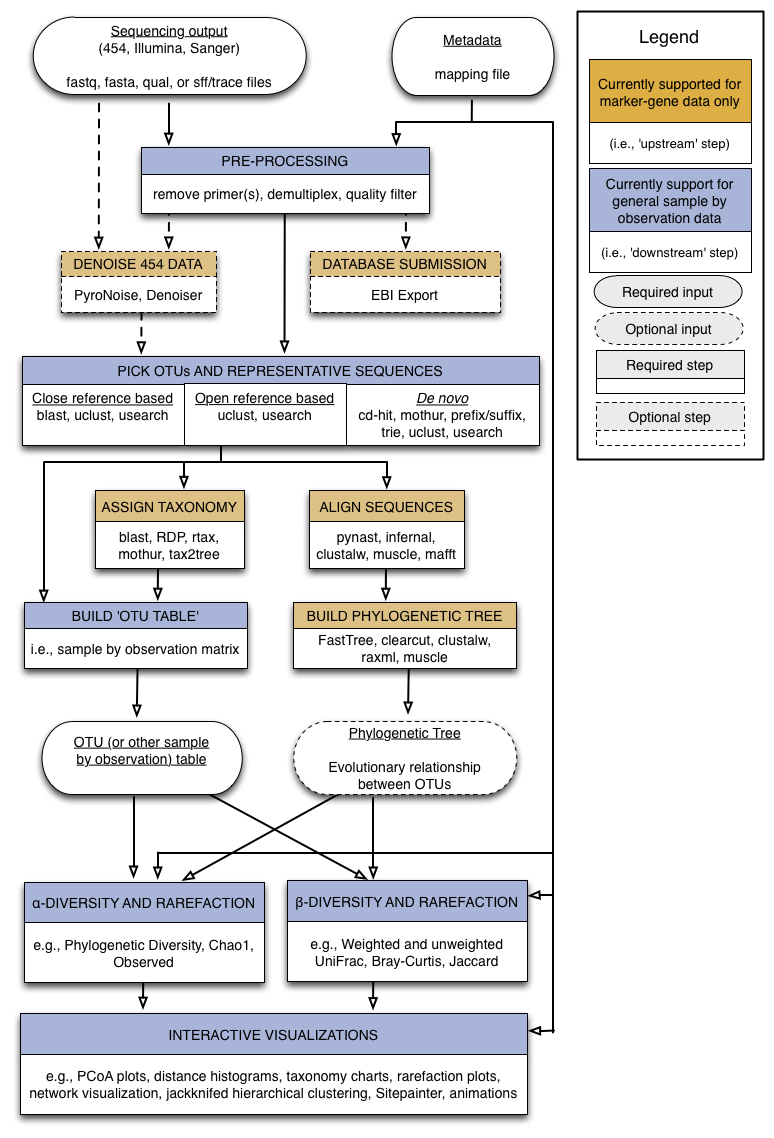
\includegraphics[width=0.75\columnwidth]{chapter_book_figures/Figure_1.jpg}
\caption[\gls{qiime} workflow overview]{\textbf{\gls{qiime} workflow overview.} The Upstream process (brown boxes)
includes all the steps that generate the \gls{otu} table and the phylogenetic tree. This step starts by
preprocessing the sequence reads and ends by building the \gls{otu} table and the phylogenetic tree.
The Downstream process (blue boxes) includes steps involved in analysis and interpretation of the results,
starting with the \gls{otu} table and the phylogenetic tree and ending with alpha and beta diversity analyses,
visualizations and statistics.}
\label{BFigure1}
\end{figure}

To illustrate some of the main features of \gls{qiime}, together with some of the analyses that can be
performed outside \gls{qiime}, we use an example dataset consisting of samples from different body sites
of 12 mice: the oral cavity, ileum, cecum, colon, fecal pellet, skin and whole mouse sample by homogenizing
the mouse carcass. 7 mice were wild type genotype (WT from here so on), while the 5 remaining mice were
transgenic (TG from here so on). The samples were collected by students during the IQ-Bio course taught by
Manuel Lladser and Rob Knight during Spring 2013 at University of Colorado at Boulder (course identifiers:
APPM5720-001-2013, CHEM4751-001-2013, CHEM5751-001-2013, CSCI4830-006-2013, CSCI7000-006-2013, MCDB6440-001-2013).

\subsubsection{Upstream analysis steps}

The \gls{qiime} analysis workflow starts with the sequencing output (fastq files), and a user-generated
mapping file. The mapping file contains information for understanding what is in each sample and is
therefore critical for performing the rest of the analyses; it is in tab-delimited text format. The main
information in this file is a unique identifier for each sample, the barcode used for each sample, the primer
sequence used, and a description for each sample, together with additional user-defined information that is
necessary for understanding the results such as which species the sample was taken from, which site on the
body is being studied, clinical variables relevant to the study, etc. The sample identifier, barcode and
primer sequence information are required for the first step of the \gls{qiime} workflow. This preprocessing
step combines sample demultiplexing, primer removal and quality-filtering. Additional information provided
about the samples in the mapping file is helpful for later steps, especially for analyses that aggregate
the samples by these fields (for example, comparing lean to obese subjects). We therefore recommend
including as much additional data about the samples as possible (often called “sample metadata”). This
auxiliary information is also very useful for identifying contaminated samples. For example,
SourceTracker \cite{Knights2011} is a package included in \gls{qiime} that identifies the proportion
of different community sources, including contamination, in each sample based on a database of samples
from known communities.

\textbf{De-multiplexing and quality filtering.} As mentioned above, high-throughput sequencing allows
multiple samples to be combined in a single sequencing run \cite{Kuczynski2011}. However, each sequence
must then be linked back to the individual sample that it came from via a DNA barcode. The barcodes,
which are short DNA sequences unique to each sample, are incorporated into each sequence from a given
sample during PCR. \gls{qiime} uses the barcodes in the mapping file to demultiplex, i.e. to assign the
sequences back to the samples they are derived from, using error-correcting codes where available
(as noted above). \gls{qiime} is also able to demultiplex variable-length barcodes such as those used in
the \gls{hmp}: see Variable-length barcodes in Other features below.

During demultiplexing, \gls{qiime} removes the barcodes and primer sequences because they are not needed
in later steps. Thus, the result after demultiplexing is a sequence matching the amplified 16S \gls{rrna} gene.

The third part of preprocessing is quality-filtering. Quality-filtering improves diversity estimates with
Illumina sequencing substantially \cite{Bokulich2013}. Illumina instruments, like most sequencing instruments,
generate a quality score for each nucleotide (Phred), related to the probability that each nucleotide was
read incorrectly. \gls{qiime} uses the Phred score and user-defined parameters to remove sequence reads
that do not meet the desired quality. These user-defined parameters are: the percentage of consecutive
high quality base calls ($p$), the maximum number of consecutive low quality base calls ($r$), the
maximum number of ambiguous bases (typically coded as N) ($n$) and the minimum Phred quality score ($q$).
For a detailed discussion of how these parameters affect diversity results, see \cite{Bokulich2013}.
This study recommends standard values for these parameters as $r = 3$, $p = 75\%$, $q = 3$ and $n = 0$,
which are the default values in the \gls{qiime} pipeline. However, the optimal values for these parameters
can vary both for individual sequencing runs and for different downstream analyses: for example,
analyses such as machine learning benefit from larger numbers of low-quality sequences, whereas accurate
counts of \gls{otu}s from a mock community require fewer, higher-quality sequences. Table~\ref{btable1} contains
an overview of the guidelines presented in \cite{Bokulich2013} for tuning these parameters to a given dataset.


\begin{sidewaystable}[htbp]
\centering
\caption[Overview of the guidelines to tune up the quality filtering parameters (adapted from \cite{Bokulich2013})]{Overview of the guidelines to tune up the quality filtering parameters.}\label{btable1}
\begin{tabular*}{\textwidth}{ccccc}
\toprule
Dataset characteristics & q & p & r & Results\\
\midrule
Majority of high-quality, & \multirow{2}{*}{increase} & \multirow{2}{*}{increase} & \multirow{2}{*}{-} & Retrieving full-length sequences with low error rates,\\
full-length sequences & & & & increasing the discovery rate of rare \gls{otu}s\\
\midrule
Short reads, or reads truncated & \multirow{2}{*}{-} & \multirow{2}{*}{lower} & \multirow{2}{*}{increase} & Retain lower-quality but\\
by early low-quality base calls & & & & taxonomic usefult reads\\
\midrule
Maximize read count for machine- & \multirow{3}{*}{-} & \multirow{3}{*}{lower} & \multirow{3}{*}{-} & \multirow{3}{*}{Increased sample size}\\
learning tools, cross-metadata & & & & \\
\gls{otu} counts comparison, etc & & & & \\
\bottomrule
\end{tabular*}
\end{sidewaystable}

The Illumina quality filtering approach differs in its fundamental principles from
454 denoising \cite{Quince2009, Reeder2010}. 454 denoising is based on flowgram
clustering \cite{Quince2009, Quince2011} and is primarily targeted at reducing
homopolymer runs, which are not a problem on the Illumina platform to the same extent.
In contrast, the Illumina quality filtering is based on a per-base Phred quality score
and does not target indels.

The \gls{qiime} quality filtering process works as follows. Starting at the
beginning of the sequence, \gls{qiime} checks that the next $r$ Phred values exceed
the user-defined quality threshold $q$. If the test is positive, it continues
slicing the window of $r$ bases until the test fails, or the end of the sequence
is reached. The sequence is then trimmed to the last base that met the quality
threshold. The next test determines whether the length of the trimmed sequence
exceeds $p$, expressed as the percentage of length of the raw sequence. If this
check fails, the sequence is excluded. Otherwise, \gls{qiime} performs the last
check on the sequence, which counts the number of ambiguous characters (N) in the
trimmed sequence and checks that it is less than $n$. If the test fails, the
sequence is rejected. \gls{qiime} combines the de-multiplexing, primer removal and
quality filtering processes in a single script, split\_libraries\_fastq.py:

\begin{lstlisting}[language=bash]
split_libraries_fastq.py
  -i $PWD/IQ_Bio_16sV4_L001_sequences.fastq.gz \
  -b $PWD/IQ_Bio_16sV4_L001_sequences_barcodes.fastq.gz \
  -m $PWD/IQ_Bio_16sV4_L001_map.txt -o $PWD/slout \
  --rev_comp_mapping_barcodes
\end{lstlisting}

In our example dataset, we used the --rev\_comp\_mapping\_barcodes option in order
to indicate that the barcodes present in the mapping file are reverse complements of
Golay 12 barcodes. We used the recommended default parameters for quality filtering
on this dataset. However, to change the values for the $r$, $p$, $n$ and $q$ quality
filtering parameters, we can use the $-r$, $-p$, $-n$ and $-q$ options to the script.
This command will write a FASTA-formatted file in the slout folder, called seqs.fna,
which contains the demultiplexed sequences that pass the quality filter. Each sequence
contains the information about which sample it came from encoded in the name of the sequence.

Multiple lanes of Illumina fastq data can be processed together in a single call
to the script, just by passing the sequence files, the barcode files and the mapping
files in the same order to the $-i$, $-b$ and $-m$ options, respectively. For example,
with two lanes, the command would look like:

\begin{lstlisting}[language=bash]
split_libraries_fastq.py
  -i sequences1.fastq,sequences2.fastq
  -b sequences1_barcodes.fastq,sequences2_barcodes.fastq
  -m mapping1.txt,mapping2.txt -o slout
\end{lstlisting}

The user can check how many sequences have been demultiplexed and passed quality-filtering
by using the count\_seqs.py command. This command also shows the mean and standard
deviation of the sequence length:

\begin{lstlisting}[language=bash]
count_seqs.py -i $PWD/slout/seqs.fna

12687021 :slout/seqs.fna (Sequence lengths (mean +/- std):
150.9989 +/- 0.1715)

12687021 : Total
\end{lstlisting}

\textbf{\gls{otu} picking.} The next step is clustering the preprocessed sequences
into \gls{otu}, which in traditional taxonomy represent groups of organisms defined by
intrinsic phenotypic similarity that constitute candidate taxa \cite{Sneath1973, Sokal1963}.
For DNA sequence data, these clusters, and hence the \gls{otu}s, are formed based on sequence
identity. In other words, sequences are clustered together if they are more similar than a
user-defined identity threshold, presented as a percentage ($s$). This level of threshold
is traditionally set at 97\% of sequence similarity, conventionally assumed to represent
bacterial species \cite{Drancourt2000}; other levels approximately represent other taxa,
although the fit between molecular data and traditional taxonomy varies for different taxa.
\gls{qiime} supports three approaches for \gls{otu} picking (de novo, closed-reference and open-reference),
and multiple algorithms for each of these approaches (Table ~\ref{btable2}). The de novo
approach (Figure ~\ref{bfigure2}a) groups sequences based on sequence identity. The closed-reference approach
(Figure ~\ref{bfigure2}b) matches sequences to an existing database of reference sequences. If a sequence fails
to match the database, it is discarded. The open-reference approach (Figure ~\ref{bfigure2}c) also
starts with an existing database and tries to match the sequences against them. However, if a
sequence does not match the database, it is added to the database as a new reference sequence.

\begin{table}[htbp]
\tiny
\centering
\caption[Supported \gls{otu} picking methods in \gls{qiime}, with a brief description of the algorithm employed and in which \gls{otu} picking approach can be used.]{Supported \gls{otu} picking methods in \gls{qiime}, with a brief description of the algorithm employed and in which \gls{otu} picking approach can be used.}\label{btable2}
\renewcommand{\arraystretch}{0.6}% Tighter
\begin{tabular*}{\textwidth}{cccccc}
\toprule
Method & \multicolumn{3}{c}{Picking approach} & Description & Reference \\
\midrule
& de & closed & open & & \\
& novo & reference & reference & & \\
\midrule
\multirow{2}{*}{cd-hit} & \multirow{2}{*}{Yes} & \multirow{2}{*}{-} & \multirow{2}{*}{-} & Applies a "longest-sequence-first list & \multirow{2}{*}{\cite{Li2006, Li2001}}\\
& & & & removal algorithm" to cluster sequences & \\
\midrule
\multirow{3}{*}{Mothur} & \multirow{3}{*}{Yes} & \multirow{3}{*}{-} & \multirow{3}{*}{-} & Takes an aligned set of sequences and clusters & \multirow{3}{*}{\cite{Schloss2009}}\\
& & & & them using a nearest-neighbor, furthest-neighbor & \\
& & & & or average-neighbor algorithm. & \\
\midrule
\multirow{2}{*}{prefix/suffix} & \multirow{2}{*}{Yes} & \multirow{2}{*}{-} & \multirow{2}{*}{-} & Clusters sequences which are identical & \multirow{2}{*}{\gls{qiime} team, unpublished}\\
& & & & in their first and/or last bases. & \\
\midrule
\multirow{3}{*}{Trie} & \multirow{3}{*}{Yes} & \multirow{3}{*}{-} & \multirow{3}{*}{-} & Clusters sequences which are identical sequences & \multirow{3}{*}{\gls{qiime} team, unpublished}\\
& & & & and sequences which are subsequences & \\
& & & & of other sequences. & \\
\midrule
\multirow{2}{*}{blast} & \multirow{2}{*}{-} & \multirow{2}{*}{Yes} & \multirow{2}{*}{-} & Compares and clusters each sequence against & \multirow{2}{*}{\cite{Altschul1990}}\\
& & & & a reference database of sequences. & \\
\midrule
\multirow{2}{*}{uclust} & \multirow{2}{*}{Yes} & \multirow{2}{*}{Yes} & \multirow{2}{*}{Yes} & Creates seed sequences which generate & \multirow{2}{*}{\cite{Edgar2010}}\\
& & & & clusters based on percent identity. & \\
\midrule
\multirow{4}{*}{usearch} & \multirow{4}{*}{Yes} & \multirow{4}{*}{Yes} & \multirow{4}{*}{Yes} & Creates seed sequences which generate & \multirow{4}{*}{\cite{Edgar2010}}\\
& & & & clusters based on percent identity, filters low & \\
& & & & abundance clusters and performs de novo and & \\
& & & & reference based chimera detection. & \\
\bottomrule
\end{tabular*}
\end{table}
\renewcommand{\arraystretch}{1}% Restore original value

\begin{figure}[htbp]
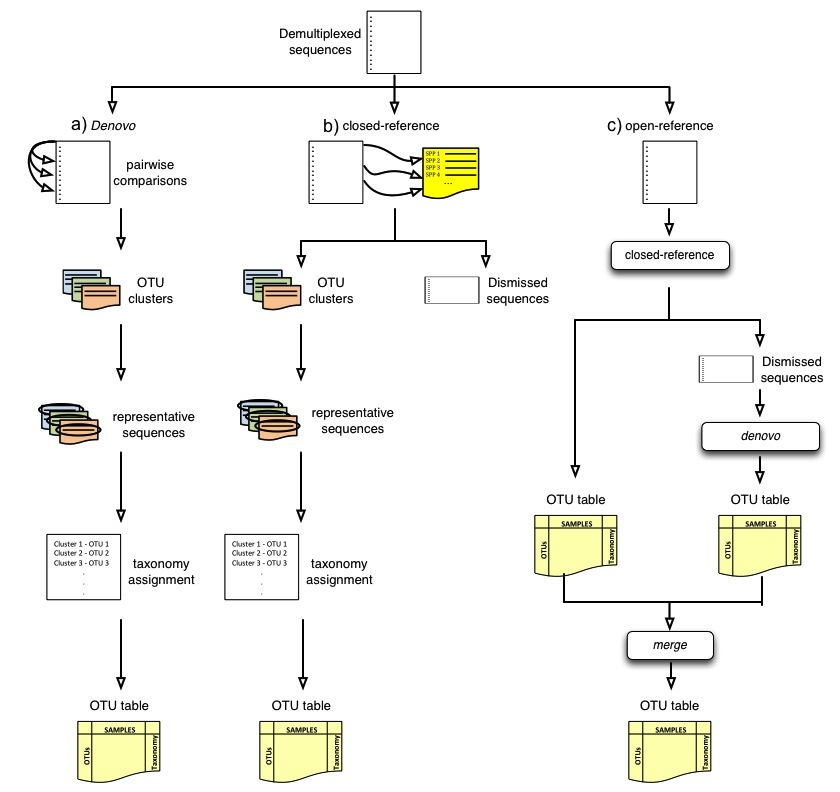
\includegraphics[width=0.75\columnwidth]{chapter_book_figures/Figure_2.jpg}
\caption[Cartoon representation of the \gls{otu} picking approaches]{\textbf{Cartoon representation of the \gls{otu} picking approaches.}
(a) de novo, (b) closed-reference and (c) open reference \gls{otu} picking respectively.
In the de novo method, sequences are compared to each other and then clusters are formed.
In the closed-reference method, sequences are compared directly to a reference dataset (e.g. GreenGenes).
Sequences that match a reference sequence are clustered; the remaining sequences are discarded. I
both \gls{otu} picking methods, once clusters are formed, a representative sequence is selected and
then taxonomy is assigned to that sequence (and applied to the rest of the sequences that make up the \gls{otu}).
Open-reference combines the closed-reference and open-reference methods. The first step is identical to
closed-reference, sequences discarded in the first step are clustered into \gls{otu}s by the de novo method,
and both \gls{otu} tables are merged into a single final \gls{otu} table. De novo and open-reference cluster all
the sequences, but closed-reference allows better comparisons between studies, especially those using
different primers, because all \gls{otu}s occur in a common reference space.}
\label{bfigure2}
\end{figure}

The \gls{otu} picking strategies shown in Figure ~\ref{bfigure2} are built on top of
algorithms for de novo clustering. Of the various algorithms available, the furthest-neighbor,
average-neighbor or nearest neighbor in mothur \cite{Schloss2005, Schloss2009} (also named
complete linkage, average linkage, and single linkage respectively) are the most widely used.
Furthest-neighbor requires that each sequence is closer than the distance threshold to
every other sequence already in the \gls{otu} (Figure ~\ref{bfigure3}). Average-neighbor requires
that the average pairwise distance of all sequences in the \gls{otu} is closer than the
distance threshold. Nearest-neighbor requires that each sequence is closer than the
distance threshold to any sequence already in the \gls{otu}. Because these three algorithms
are variants on hierarchical clustering, they require loading the distance matrix
(proportional to the square of the number of dereplicated sequences) into memory, and are
therefore challenging to apply to large datasets (e.g., larger than 105 sequences). The
\gls{otu}s yield by these three algorithms also change their memberships at different sequencing depths
(i.e. the number of sequences chosen for clustering), which can be a problem for estimates of total
\gls{otu} numbers \cite{Roesch2007}.

\begin{figure}[htbp]
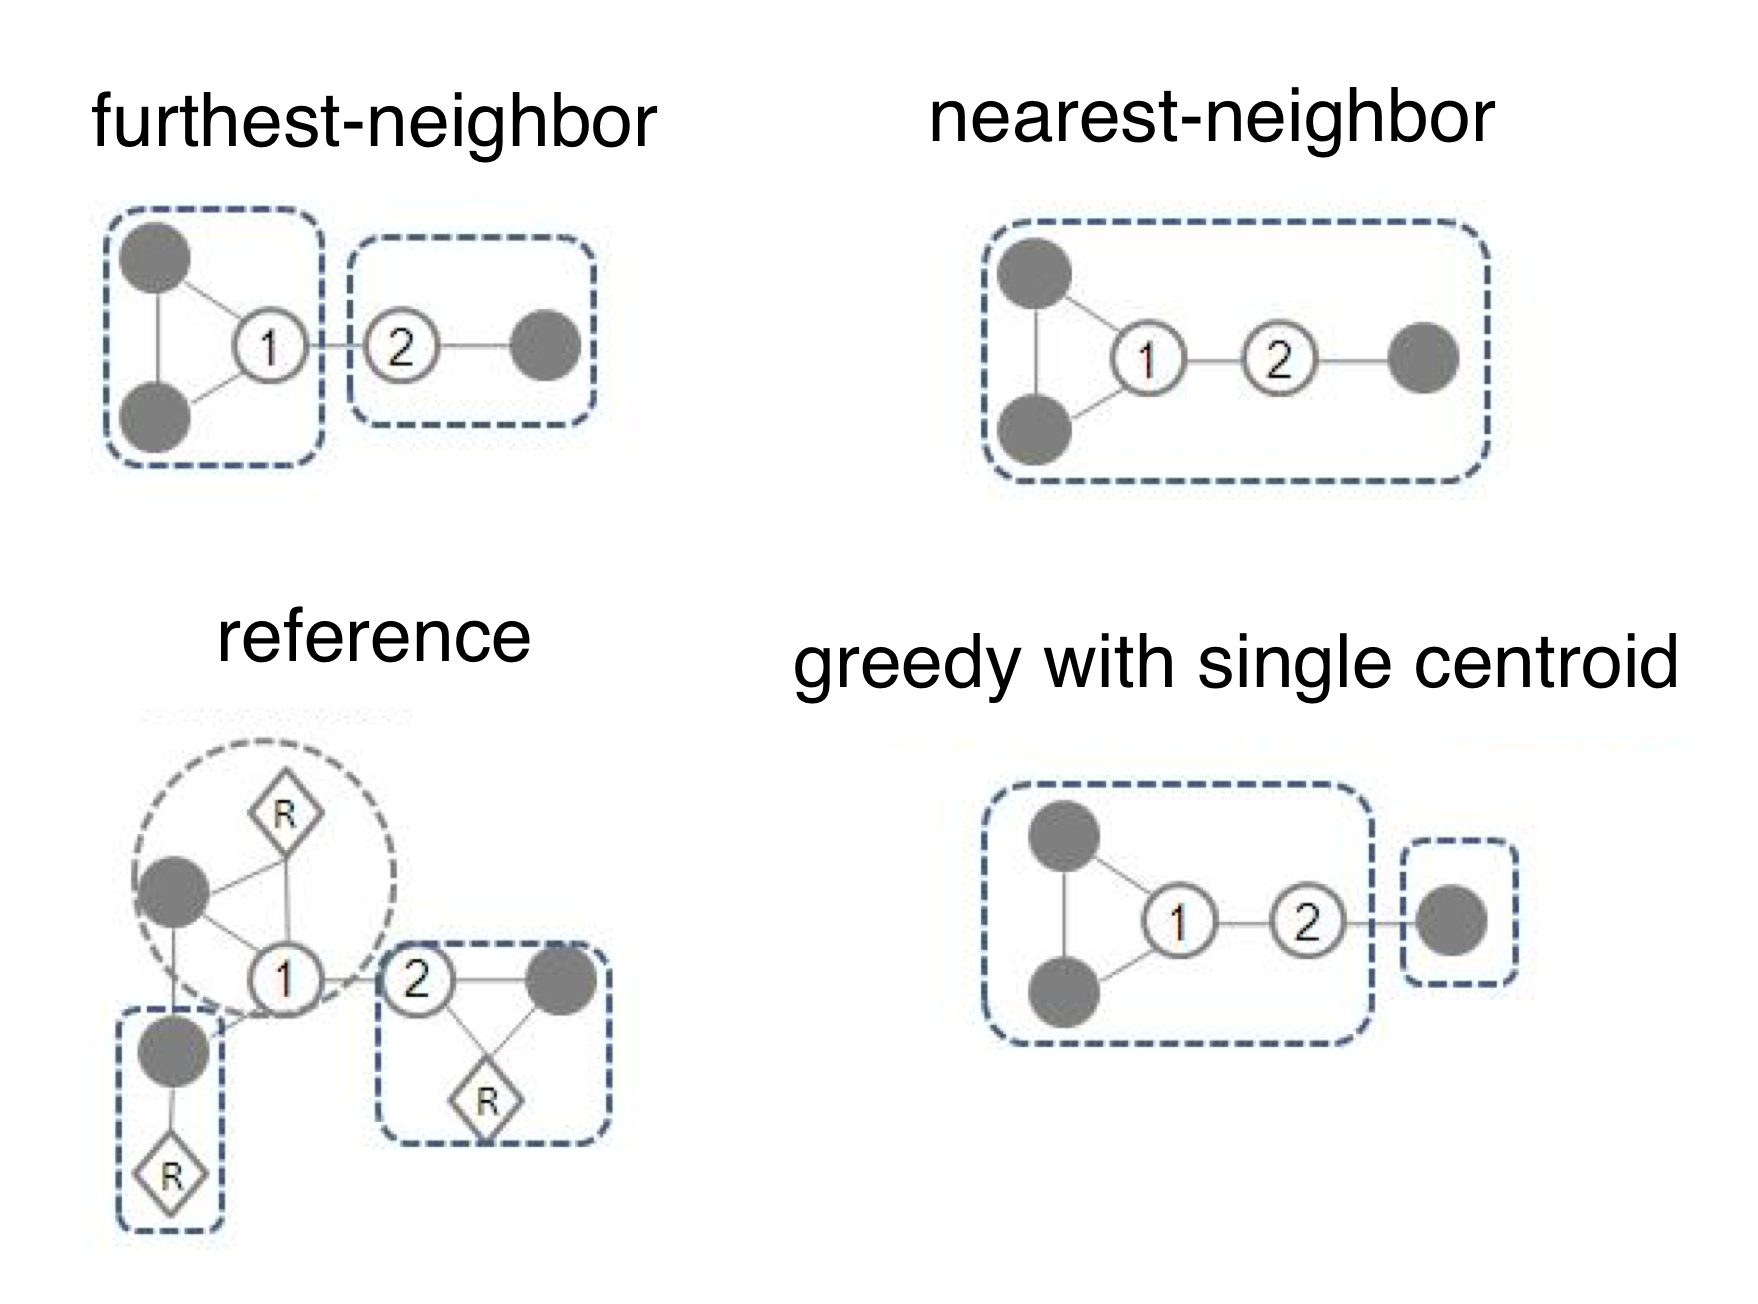
\includegraphics[width=0.75\columnwidth]{chapter_book_figures/Figure_3.jpg}
\caption[Cartoon demonstrating different clustering algorithms]{\textbf{Cartoon demonstrating different clustering algorithms.}
Circles representing sequences linked with lines are within the distance threshold.
The two numbered sequences are the first and second sequences in order in the file.
The reference algorithms only consider the distance between reference (R) and sequences.}
\label{bfigure3}
\end{figure}

A solution to the distance matrix problem comes from uclust and usearch, which are
greedy algorithms based on using a single centroid in each \gls{otu} \cite{Edgar2010}.
The centroid could be either from a reference database (usearch) or identified de
novo from the sequence dataset (both uclust and usearch) (Figure ~\ref{bfigure3}).
Sequences are serially compared to centroids in a user-defined order (usually decreasing
abundance). If a sequence falls within the distance threshold of more than one centroid,
the new sequence can either be grouped with the first centroid encountered, or the one
with the closest distance. Both uclust and usearch are much more efficient than the
hierarchical methods, and they do not need to load a large distance matrix into memory
(although recent versions of mothur also avoid the constraint of loading the full
distance matrix). usearch is the default de novo \gls{otu} picking method in \gls{qiime}.
Note that it is essential to note both your \gls{otu} picking strategy, and, if de novo
\gls{otu} picking is used, which algorithm you used to do it: it is not sufficient
simply to state that you used a 97\% threshold.

Because the \gls{otu} picking approach selection is a critical point in microbial
community analysis, the \gls{qiime} team has produced a detailed document that
describes the \gls{otu} picking protocols, their advantages and limitations
\footnote{\url{https://github.com/qiime/qiime/blob/master/doc/tutorials/otu_picking.rst}}.
Table ~\ref{btable3} compares the different \gls{otu} picking approaches and gives
guidelines for choosing an appropriate \gls{otu} picking strategy.

\begin{table}[htbp]
\tiny
\centering
\caption[\gls{otu} picking approaches comparison. The table shows when each of the \gls{otu} picking approaches should be used and when they cannot be applied. It briefly describes the advantages and disadvantages of using each of the \gls{otu} picking approaches.]{\gls{otu} picking approaches comparison. The table shows when each of the \gls{otu} picking approaches should be used and when they cannot be applied. It briefly describes the advantages and disadvantages of using each of the \gls{otu} picking approaches.}\label{btable3}
\renewcommand{\arraystretch}{0.5}% Tighter
\begin{tabular*}{\textwidth}{cccc}
& de novo & closed reference & open reference\\
\toprule
Must   & There is no reference          & Comparing non-overlapping. & -\\
use if & sequence collection to         & amplicons. The reference & \\
       & cluster against (e.g.          & set of sequences must span & \\
       & infrequently used              & both of the regions & \\
       & marker gene)                   & being sequenced & \\
\midrule
Cannot & Comparing non-overlapping   & There is no reference    & Comparing non-overlapping \\
use if & amplicons (e.g. V2 and      & sequence collection      & amplicons (e.g. V2 and V4\\
       &  V4 regions of 16S \gls{rrna})    & to cluster against & regions of 16S \gls{rrna}). There \\
       &                             & (e.g. infrequently       & is no reference sequence\\
       &                             & used marker gene)        & collectionto cluster against (e.g.\\
       &                             &                          & infrequently used marker gene)\\
\midrule
Pros & All reads are clustered & Fast, as it is fully parallelizable    & All reads are clustered.\\
     &                         & (useful for extremely large datasets). & Fast, as is partially run on parallel.\\
     &                         & Better tree and taxonomy quality & \\
     &                         & since the \gls{otu}s are already defined & \\
     &                         & on the reference set. & \\
\midrule
Cons & Time consuming since it runs in         & Inability to detect novel      & There are still some steps\\
     & serial respect to the reference         & diversity with respect to      & performed in serial. If the\\
     & set because the reads that don’t        & the reference set because      & data set contains a lot of\\
     & hit the reference sequence collection   & the reads that don’t hit       & novel diversity with respect\\
     &  are discarded, so the analysis         & the reference sequence         & to the reference set, this\\
     & focus on the “already known” diversity. & collection are discarded,      & can still be slow.\\
     & If the studied environment is not       & so the analysis focus on       &\\
     & well-characterized, a large fraction    & the “already known” diversity. &\\
     & of the reads can be thrown away         & If the studied environment is  &\\
     &                                         & not well- characterized, a     &\\
     &                                         & large fraction of thereads     &\\
     &                                         & can be thrown away             &\\
\bottomrule
\end{tabular*}
\end{table}
\renewcommand{\arraystretch}{1}% Restore original value

The recommended \gls{otu} picking approach is open-reference \gls{otu} picking,
because this approach provides the best trade-off between the time taken to complete
the analysis and the ability to discover novel diversity.

Once the sequences have been clustered into \gls{otu}s, a representative sequence
is picked for each \gls{otu}. The entire cluster will thus be represented by a single
sequence, speeding up subsequent steps (because redundant sequences need not be
considered). \gls{qiime} allows the representative sequence to be selected using
several techniques: choosing a sequence at random, choosing the longest sequence,
the most abundant sequence or the first sequence. If using uclust or usearch \cite{Edgar2010},
the cluster seed will be used as the representative sequence. The default behavior
in \gls{qiime} is to use the most abundant sequence in each \gls{otu} as the
representative sequence, because these sequences are least likely to represent
sequencing errors (for other applications, such as clustering with near-full-length
Sanger sequences, it may be more desirable to pick the longest sequence instead).
In case of closed-reference \gls{otu} picking, sequences from the reference collection
should be used as the representative sequences, which is the default behavior when
the closed-reference approach is selected.

\textbf{Identify chimeric sequences.} During the \gls{pcr} amplification process,
some of the amplified sequences can be produced from multiple parent sequences,
generating sequences known as chimeras. Although these sequences are technical
artifacts rather than representing actual members of the community, chimeric sequences
are important for alpha diversity estimates (although they are less important for
cross-sample comparisons, because each chimera is relatively rare and the same
chimera is unlikely to be generated systematically in different samples \cite{Ley2008}.
However, the same chimera can sometimes be generated in multiple \gls{pcr} reactions:
for example, Haas et al. \cite{Haas2011} reported that chimeric sequences formed
from Streptococcus and Staphylococcus occurred multiple times independently, so
presence of the same sequence in multiple \gls{pcr} does not mean that it is not chimeric.

\gls{qiime} currently supports three different methods for detecting chimeras: blast
fragments, a \hspace{0.01cm} taxonomy-assignment-based \hspace{0.01cm} approach \hspace{0.01cm} using \hspace{0.01cm} BLAST \cite{Altschul1990};
ChimeraSlayer \cite{Haas2011}, which uses BLAST to identify potential chimera parents;
and usearch 6.1 \cite{Edgar2010}, which can perform de novo chimera detection based on
abundances as well as reference-based chimera detection. The recommended method for
identifying chimeric sequences is uchime \cite{Edgar2011}, which is integrated in
the usearch 6.1 \cite{Edgar2010} pipeline. Uchime is the fastest method for detecting
chimeric sequences and it is executed by default if the usearch method is selected
for picking \gls{otu}.

\textbf{Taxonomy assignment.} The next step in the \gls{qiime} workflow is to
assign the taxonomy to each sequence of the representative set. This step connects
the \gls{otu}s to named organism, which is useful for inferring likely functional roles
for members of the community. When using a closed-reference approach for \gls{otu} picking,
the taxonomy of the sequences can be pulled out from the reference set. In case of
the open-reference and de novo approaches, because the clusters are not created from
any reference database (as a reminder, in the open-reference approach, sequences that
fail to cluster to the reference database form new clusters), the taxonomy should be
assigned using a reference dataset. We recommend the GreenGenes database
\cite{DeSantis2006, McDonald2012} as the default reference data set for assigning
taxonomy, although the RDP \cite{Cole2009} and Silva \cite{Quast2013} databases also
have strengths and weaknesses relative to GreenGenes and should be considered for some
analyses. Silva includes microbial eukaryotes and has invested substantial effort in
cleaning up marine taxa; RDP has close links to formally recognized names in taxonomy,
which can be especially useful for medical microbiology. \gls{qiime} can assign taxonomy
against any of the given databases, or against a custom database, using several
methods: BLAST \cite{Altschul1990}, RDP Classifier \cite{Wang2007}, rtax \cite{Soergel2012},
mothur \cite{Schloss2009} and tax2tree \cite{McDonald2012}. The \gls{qiime} team recommends
the RDP classifier method \cite{Wang2007} with a confidence value of 0.8. However, if
the user has paired-end reads, the best method to use is the rtax \cite{Soergel2012}, and
the user should provide the fasta files with both the first and second read from the
paired-end sequencing. Note that the taxonomy assignment method and the reference database
must both be described in order for an analysis to be reproducible, and that these methods
can have a larger effect on taxonomy than the underlying biological sample, so it is important
to be consistent \cite{Liu2008}.

\textbf{Sequence alignment.} The next step in the \gls{qiime} workflow is to align the
sequences. The sequences must be aligned to infer a phylogenetic tree, which is used for
diversity analyses and to understand the relationships among the sequences in the sample.
Currently, \gls{qiime} supports the following methods for performing sequence alignment:
PyNAST \cite{Caporaso2010PyNAST}, Infernal \cite{Nawrocki2009}, clustalw \cite{Larkin2007},
muscle \cite{Edgar2004} and mafft \cite{Katoh2002}. The recommended (and default) method is
PyNAST \cite{Caporaso2010PyNAST}. This method aligns the sequences against a template sequence
alignment, for which we recommend the GreenGenes core set \cite{DeSantis2006}.

When sequences do not align well using PyNAST, the Infernal package \cite{Nawrocki2009}
should be used. Like PyNAST, it requires a template alignment, but unlike PyNAST, it uses
\gls{scfg} to align incorporating secondary structure. Although this method is slow compared
to other methods, it does takes advantage of RNA secondary structure (provided in a
Stockholm-format file) and can be useful for aligning more variable \gls{rrna}s. For marker
genes other than \gls{rrna} genes, the best strategy for building phylogenetic trees is to align
the protein sequences (if available) using MUSCLE.

\textbf{Phylogeny construction.} This step in the \gls{qiime} workflow infers a
phylogenetic tree from the multiple sequence alignment generated by the previous step.
The phylogenetic tree represents the relationships among sequences in terms of the
amount of sequence evolution from a common ancestor. This phylogenetic tree is used
in many downstream analyses, such as the UniFrac metric \cite{Lozupone2005} for beta diversity.

The current methods supported for inferring the phylogenetic tree in \gls{qiime} are
FastTree \cite{Price2009}, clearcut \cite{Evans2006}, clustalw \cite{Larkin2007},
raxml \cite{Stamatakis2005} and muscle \cite{Edgar2004}. The default and recommended
method in \gls{qiime} is the FastTree \cite{Price2009} method because it shows the
best trade-off between run time and reliability of the inferred tree.

\textbf{Make \gls{otu} table} The last part of the upstream stage in \gls{qiime} is to
construct the \gls{otu} table. The \gls{otu} table is a sample by observation matrix
that also includes the taxonomic prediction for each \gls{otu}. For the \gls{otu} table
representation, \gls{qiime} uses the Genomics Standards Consortium candidate standard \gls{biom}
format \cite{McDonald2012BIOM}. The \gls{otu} table, the mapping file and the phylogenetic
tree, are the main files for performing the downstream analysis.

\gls{qiime} can perform all the steps for generating the \gls{otu} table and the
phylogenetic tree from the preprocessed data in a single command. There is a separate
command for each \gls{otu} picking approach. In the following commands, we assume that
the GreenGenes reference files \cite{DeSantis2006} are located in the current directory.
As a remainder, our seqs.fna has 12.687.021 sequences of length 150.9989 +/- 0.1715:

\begin{itemize}
    \item For de novo (run time ∼80 hours on 1 processor (not parallelizable)):
    \begin{lstlisting}[language=bash]
    pick_de_novo_otus.py -i $PWD/slout/seqs.fna \
      -o $PWD/denovo_otus
    \end{lstlisting}
    \item For closed-reference (run time ∼2 hours on 20 processors):
    \begin{lstlisting}[language=bash]
    pick_closed_reference_otus.py
      -i $PWD/slout/seqs.fna \
      -o $PWD/closed_ref_otus \
      -r $PWD/gg_12_10_otus/rep_set/97_otus.fasta \
      -t $PWD/gg_12_10_otus/taxonomy/\
         97_otu_taxonomy.txt \
      -a -O 20
    \end{lstlisting}
    \item For open-reference (run time ∼27 hours on 20 processors):
    \begin{lstlisting}[language=bash]
    pick_open_reference_otus.py \
     -o $PWD/open_ref_otus \
     -i $PWD/slout/seqs.fna \
     -r $PWD/gg_12_10_otus/rep_set/97_otus.fasta \
     -a -O 20
    \end{lstlisting}
\end{itemize}


Because the closed-reference and open-reference \gls{otu} picking approaches can
be run in parallel, we use the $-a$ and $-O$ 20 options in order to run them using
20 processors.

\subsubsection{Downstream analysis steps}

Once we have generated the \gls{otu} table and the phylogenetic tree, we can start the
downstream analysis. At this point, we strongly recommend performing a second level
of quality-filtering, based on \gls{otu} abundance. The recommended procedure is to
discard those \gls{otu}s with a number of sequences less than 0.005\% of the total
number of sequences (see Bokulich et al. \cite{Bokulich2013} for a detailed description
of the effect of this parameter in further downstream analyses). \gls{qiime} executes the
\gls{otu} abundance quality-filtering step through the script filter\_otus\_from\_otu\_table.py:

\begin{lstlisting}[language=bash]
filter_otus_from_otu_table.py \
 -i $PWD/open_ref_otus/\
    otu_table_mc2_w_tax_no_pynast_failures.biom \
 -o $PWD/open_ref_otus/otu_table_filtered.biom \
 --min_count_fraction 0.00005
\end{lstlisting}

This step greatly reduces the problem of spurious \gls{otu}s, most of which are
present at very low abundance.

\gls{qiime} 1.7.0 allows a first-pass view of common diversity analyses using a single
command: core\_diversity\_analysis.py. One of the parameters required by this command
is the sampling depth, the number of sequences that should be included in each sample
for diversity analyses. This is required, because many of the commonly used diversity
metrics are very sensitive to the number of sequences obtained per sample, such that
samples that are similar in the number of sequences that were obtained appear similar
to one another. This is bad because the number of sequences per sample is typically
a methodological artifact, not reflective of biological reality. The sampling depth
defines the size of the random subset of sequences that will be selected for each
sample for all subsequent diversity analyses.

The optimal sampling depth is data-dependent. There is no universal way of choosing a
rarefaction level, although heuristics can be applied. For example, if most samples have
more than 10,000 sequences and the rest range from 500 to 50 sequences per sample,
it would be recommended to use 10,000 as the rarefaction level. Although many studies
show marked variation in sequence depth with only a few “bad” samples, it is not always
easy to choose the rarefaction level. We strongly recommend rarefying over 1000
sequences/sample for Illumina MiSeq, because samples below this level often suffer
from other quality issues as well.

The information needed to choose the rarefaction level can be obtained from the
script print\_biom\_table\_summary.py, which shows summary information on the
\gls{otu} table such as the number of sequences, the number of \gls{otu}s, the
number of samples and the number of counts per sample, among others:

\begin{lstlisting}[language=bash]
print_biom_table_summary.py \
 -i $PWD/open_ref_otus/otu_table_filtered.biom

Num samples: 90
Num observations: 783
Total count: 10637688.0
Table density (fraction of non-zero values): 0.4289
Table md5 (unzipped): eb0f1d7fbb50bc31695dade31db1e198
Counts/sample summary:
 Min: 1.0
 Max: 493427.0
 Median: 99111.0
 Mean: 118196.533333
 Std. dev.: 94277.5956531
 Sample Metadata Categories: None provided
 Observation Metadata Categories: taxonomy
Counts/sample detail:
 BLANK4.732555: 1.0
 BLANK5.732537: 1.0
 Joshua.Jose.WTAbd.732533: 1.0
 Nick.Krishna.TG.Fec.732513: 2.0
 TH.CVA.WT.Oral.732491: 2.0
 BLANK2.732552: 3.0
 BLANK3.732479: 5.0
 BLANK6.732470: 7.0
 Elizabeth.Chris.WT.Abd.732490: 10.0
 Uri.Jake.TGAbd.732468: 10.0
 TH.CVA.WT.Abd.732477: 13.0
 BLANK10.732524: 812.0
 Elizabeth.Chris.WT.Oral.732520: 7410.0
 Elizabeth.Chris.WT.Col.732481: 21746.0
Jordan.Lisette.TG.Ile.732463: 27149.0
 ...
 TH.CVA.WT.Fec.732553: 372327.0
 Wang.TG.Cec.732527: 396391.0
 TH.CVA.WT.Ile.732517: 493427.0
\end{lstlisting}

In the above output we can see the information contained in the \gls{otu} table resulting
from applying the open-reference \gls{otu} picking. Some of the relevant information contained
in this output is the total number of samples (90), the total number of \gls{otu}s (783),
the number of reads (10637688) and the number of \gls{otu}s per sample. Applying the above
heuristic, we could select a subsampling depth of 7410 sequences. However, because we have
run three different \gls{otu} picking approaches and we want to compare them, we must search
for the rarefaction level that best fits the three \gls{otu} tables. Below are the summarized
information for the de novo \gls{otu} table and the closed reference \gls{otu} table, respectively:

\begin{lstlisting}[language=bash]
print_biom_table_summary.py \
 -i $PWD/denovo_otus/otu_table_filtered.biom
Num samples: 93
Num observations: 600
Total count: 11122386.0
Table density (fraction of non-zero values): 0.4344
Table md5 (unzipped): b002dd85c93fd9d0571ff23b05d21dde
Counts/sample summary:
 Min: 0.0
 Max: 497234.0
 Median: 108322.0
 Mean: 119595.548387
 Std. dev.: 93487.3335598
 Sample Metadata Categories: None provided
 Observation Metadata Categories: taxonomy
Counts/sample detail:
 BLANK7.732497: 0.0
 BLANK8.732522: 0.0
 Jordan.Lisette.TG.Abd.732467: 0.0
 BLANK4.732555: 1.0
 BLANK5.732537: 1.0
 Joshua.Jose.WTAbd.732533: 1.0
 BLANK2.732552: 3.0
 Nick.Krishna.TG.Fec.732513: 3.0
 TH.CVA.WT.Oral.732491: 3.0
 BLANK3.732479: 5.0
 BLANK6.732470: 9.0
 Elizabeth.Chris.WT.Abd.732490: 10.0
 Uri.Jake.TGAbd.732468: 10.0
 TH.CVA.WT.Abd.732477: 13.0
 BLANK10.732524: 825.0
 Elizabeth.Chris.WT.Oral.732520: 7376.0
 Joey.Aaron.Kyle.WT.Abd.732541: 35655.0
 ...
 Wang.TG.Cec.732527: 394351.0
 TH.CVA.WT.Ile.732517: 497234.0

print_biom_table_summary.py \
 -i $PWD/closed_ref_otus/otu_table_filtered.biom
Num samples: 90
Num observations: 673
Total count: 9434459.0
Table density (fraction of non-zero values): 0.4250
Table md5 (unzipped): 257b528478a2700c72f979ce8d9a9a1c
Counts/sample summary:
 Min: 1.0
 Max: 347785.0
 Median: 90092.0
 Mean: 104827.322222
 Std. dev.: 78560.4683831
 Sample Metadata Categories: None provided
 Observation Metadata Categories: taxonomy
Counts/sample detail:
 BLANK4.732555: 1.0
 BLANK5.732537: 1.0
 Joshua.Jose.WTAbd.732533: 1.0
 BLANK3.732479: 2.0
 Nick.Krishna.TG.Fec.732513: 2.0
 TH.CVA.WT.Oral.732491: 2.0
 BLANK2.732552: 3.0
 Uri.Jake.TGAbd.732468: 5.0
 BLANK6.732470: 7.0
 Elizabeth.Chris.WT.Abd.732490: 10.0
 TH.CVA.WT.Abd.732477: 12.0
 BLANK10.732524: 710.0
 Elizabeth.Chris.WT.Oral.732520: 7205.0
 Elizabeth.Chris.WT.Col.732481: 22652.0
 ...
 TH.CVA.WT.Fec.732553: 329988.0
 TH.CVA.WT.Ile.732517: 347785.0
\end{lstlisting}

From the above output, we see that a reasonable rarefaction level for the three
tables is 7205 counts per sample, derived from the closed reference \gls{otu} picking.

Once the subsampling depth is chosen, we can execute the core\_diversity\_analyses.py
command over the three \gls{otu} tables. We provide the subsampling depth via the
$-e$ parameter, the \gls{otu} table via the $-i$ parameter, the mapping file through
the $-m$ parameter and the metadata categories to use in categorical analyses through
the $-c$ parameter. The $-o$ parameter is used to provide the output directory and the
$-a -O$ 64 are used to run the command in parallel using 64 processes.

\begin{lstlisting}[language=bash]
mkdir $PWD/diversity_analysis

core_diversity_analyses.py \
 -i $PWD/open_ref_otus/otu_table_filtered.biom \
 -m $PWD/IQ_Bio_16sV4_L001_map.txt \
 -t $PWD/open_ref_otus/rep_set.tre \
 -e 7205 -c GENOTYPE,BODY_SITE \
 -o $PWD/diversity_analysis/open_ref -a -O 64

core_diversity_analyses.py \
 -i $PWD/denovo_otus/otu_table_filtered.biom \
 -m $PWD/IQ_Bio_16sV4_L001_map.txt \
 -t $PWD/denovo_otus/rep_set.tre -e 7205 \
 -c GENOTYPE,BODY_SITE \
 -o $PWD/diversity_analysis/denovo -a -O 64

core_diversity_analyses.py \
 -i $PWD/closed_ref_otus/otu_table_filtered.biom \
 -m $PWD/IQ_Bio_16sV4_L001_map.txt \
 -t $PWD/gg_12_10_otus/trees/97_otus.tree \
 -e 7205 -c GENOTYPE,BODY_SITE \
 -o $PWD/diversity_analysis/closed_ref -a -O 64
\end{lstlisting}

The core\_diversity\_analyses.py command filters the \gls{otu} table before
executing the diversity analyses. The filter removes samples from the \gls{otu}
table that do not have at least the user-defined subsampling depth (7205 in our
case). This filtering removes low-coverage samples from the \gls{otu} table, because
they are not informative enough to be included in the study. After these samples
have been filtered, the script performs the rarefaction step at the given subsampling depth.

The output of this script is an HTML file that can be opened in a web browser (Figure ~\ref{bfigure4}).
This HTML file gives access to the results of the different diversity analysis performed
(taxa summaries, $\alpha$-diversity, $\beta$-diversity and category significance)
which will be explained in further sections.

\begin{figure}[htbp]
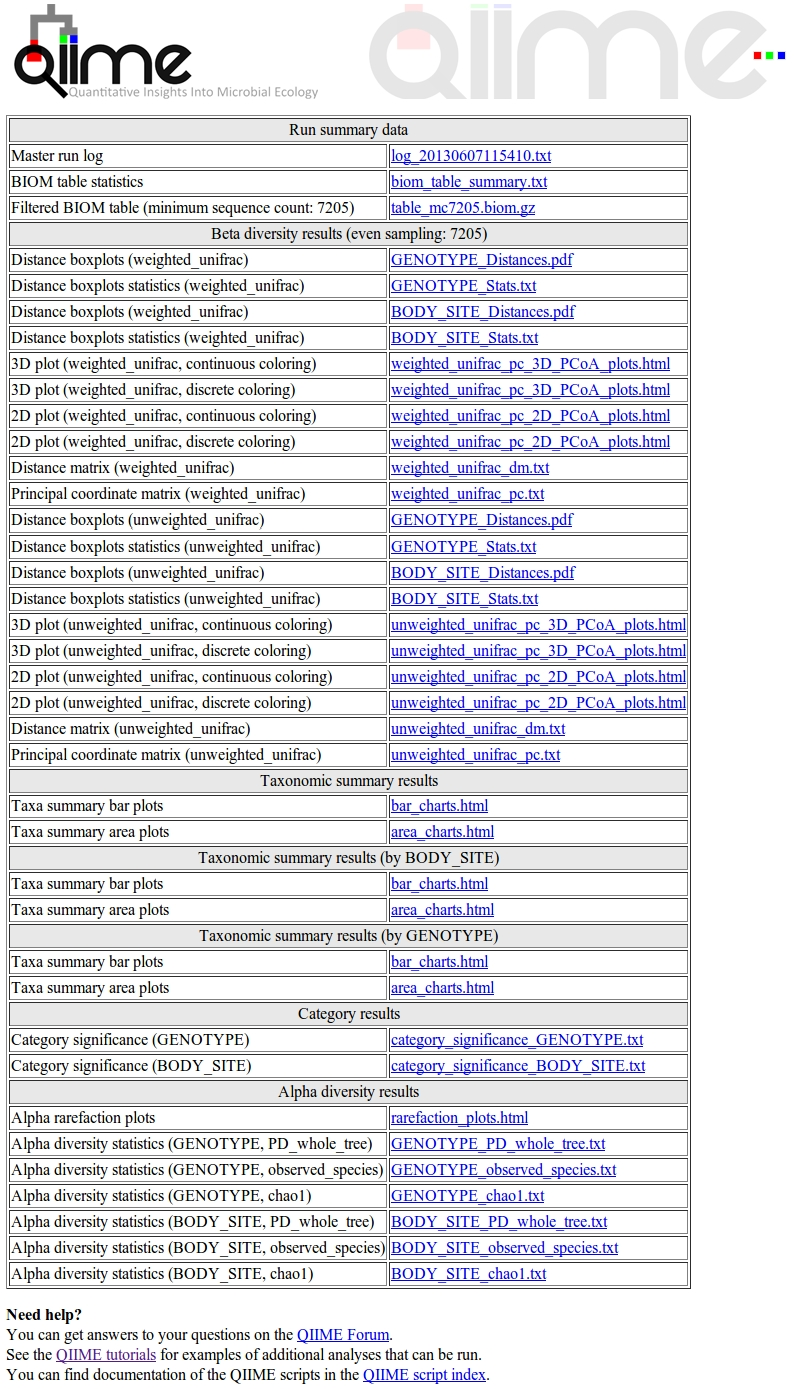
\includegraphics[width=0.75\columnwidth]{chapter_book_figures/Figure_4.jpg}
\caption[HTML result from core\_diversity\_analyses.py]{\textbf{HTML result from core\_diversity\_analyses.py.}
This HTML file summarizes and gives access to the results of the diversity analyses conducted on the given \gls{otu} table}
\label{bfigure4}
\end{figure}

For the following downstream analysis we have used the \gls{otu} table and phylogenetic
tree resulting from the open-reference \gls{otu} picking approach. In cases where we
are performing comparisons between \gls{otu} picking approaches, we will specify
which approaches we have used.

\textbf{Taxa summaries.} One way to visualize the \gls{otu}s in each sample is a taxa
summary, which summarizes the relative abundance of the taxa present in a set of
samples on multiple taxonomic levels (e.g. phylum, order, etc.) (see Figure ~\ref{bfigure5}).
This provides a quick way to identify samples that may be drastically different from others
(i.e. outliers), and visually identify expected patterns and differences between and among samples.
For example, this tool can be used to identify patterns such as differences in the
relative abundance of Firmicutes and Bacteroidetes in the gut microbiomes of lean versus
obese mice, e.g. Ley, Backhed, Turnbaugh, Lozupone, Knight, and Gordon \cite{Ley2008}.
These patterns can then be statistically tested using other methods, either within \gls{qiime} or
elsewhere. \gls{qiime} contains a workflow called summarize\_taxa\_through\_plots.py that generates
user-specified plot types, including bar, pie, and area graphs. These graphs provide a way to
visually compare the composition of each sample, or of groups of samples. An \gls{otu} table
with assigned taxonomies is the only required input file, and options allow the user
summarize across categories (using the metadata file), at different taxonomic levels, or
only using \gls{otu}s that are present at abundances higher or lower than user-defined thresholds.
The web interface allows a scroll-over feature that identifies the taxonomy of the separate taxa.
Additional output files include image files of the charts and legends, and tab-delimited files
of the calculated abundances, which can then be further filtered and manipulated for
downstream statistical analyses.

\begin{figure}[htbp]
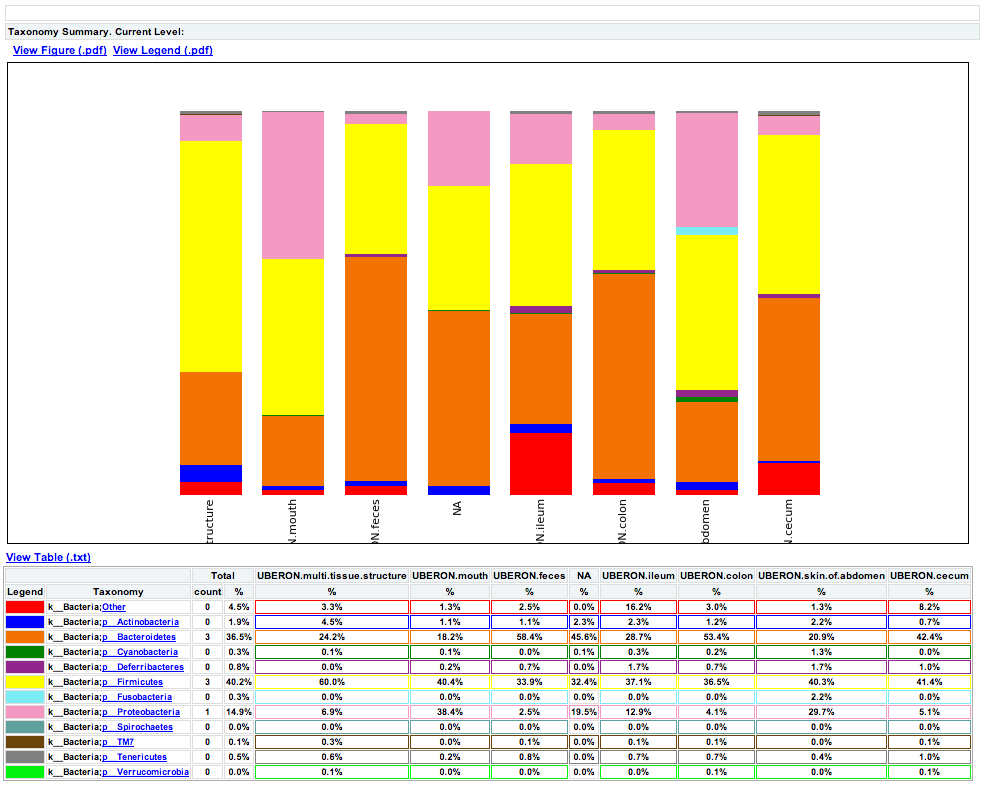
\includegraphics[width=0.75\columnwidth]{chapter_book_figures/Figure_5.jpg}
\caption[Taxa summary of the example dataset]{\textbf{Taxa summary of the example dataset.}
Samples have been grouped and averaged by body site, and taxonomic composition is shown on
the phylum level. Each column in the plot represents a body site, and each color in the column
represents the percentage of the total sample contributed by each taxon group at phylum level.
The taxa summaries plot help us to see which taxon groups are more prevalent in a sample.
For example, the fecal samples are dominated by Bacteroidetes, while mouth and skin samples
are dominated by Proteobacteria. We can also see that Fusobacteria is only present at appreciable
levels in the skin samples.}
\label{bfigure5}
\end{figure}

\textbf{Diversity analysis.} Microbial ecology studies the diversity of microorganisms
by characterizing bacterial communities in different environments, and determining the
factors that drive diversity in these communities \cite{Atlas1998}. Whittaker (1960) and
Whittaker (1972) define different types of measurements of diversity as alpha, beta and gamma
diversities. Alpha diversity is defined as the diversity of organisms in one sample or environment.
Beta-diversity is the difference in diversities across samples or environments. Finally,
gamma-diversity ($\gamma$-diversity) measures the diversity at a broader scale, such as a
province or region. Several different metrics of alpha- and beta-diversity are implemented in in
\gls{qiime} pipeline. Diversity measurements and their applications in microbial have been discussed in
detail elsewhere \cite{Jost2007, Kuczynski2010Patterns, Lozupone2008}, and here we focus on
examples of their application.

\textbf{Alpha diversity analysis.} \gls{qiime} can generate plots showing the results of
alpha diversity, allowing the user to choose the diversity metric and different
rarefaction levels (Figure ~\ref{bfigure6}). These images are often used to estimate
the true species richness of a community.

\begin{figure}[htbp]
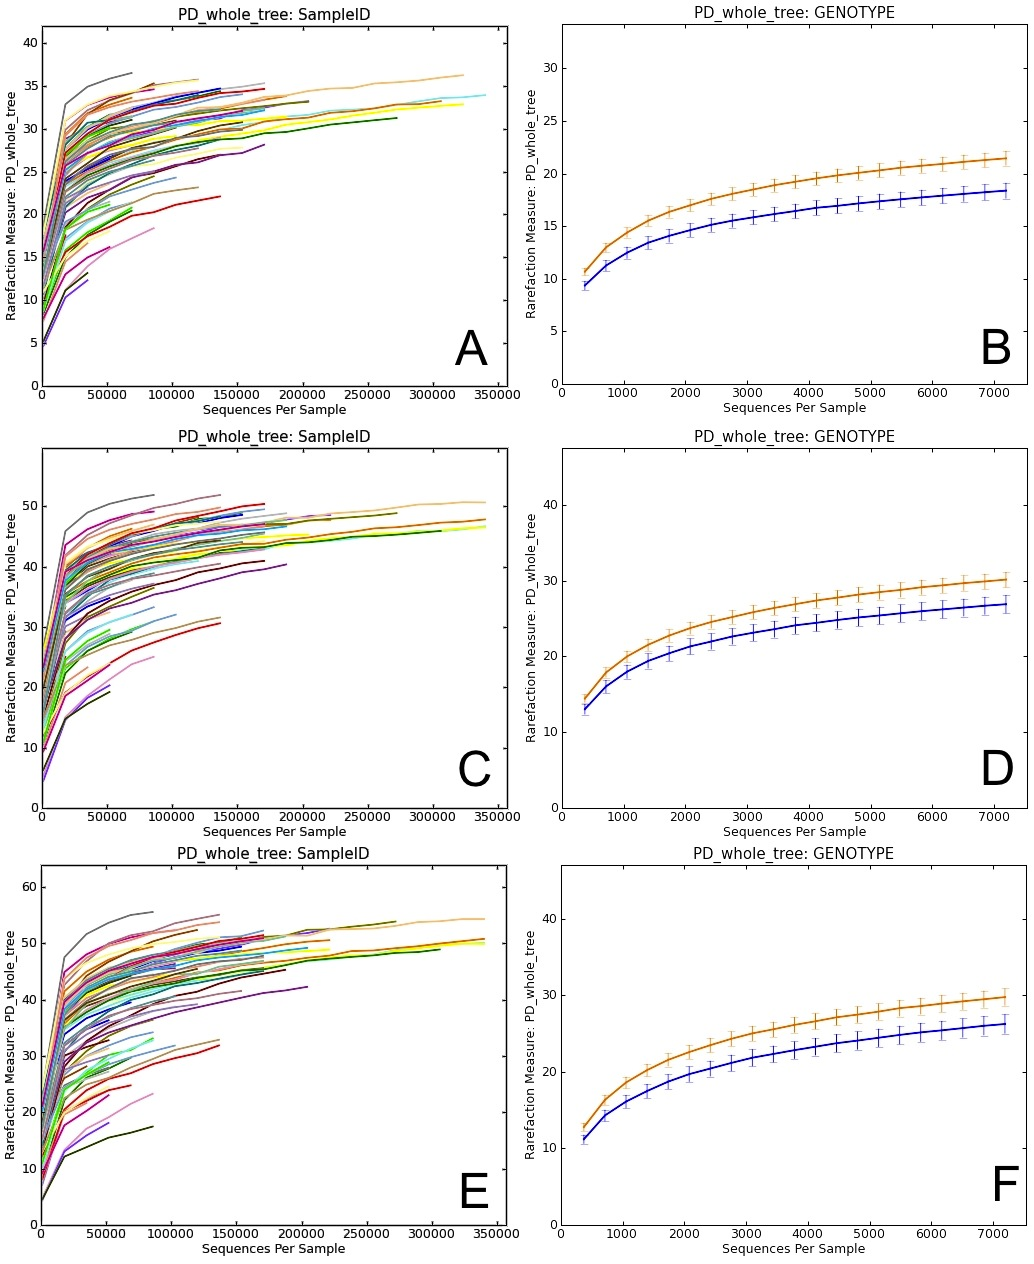
\includegraphics[width=0.75\columnwidth]{chapter_book_figures/Figure_6.jpg}
\caption[Alpha diversity curves at different rarefaction depths using different \gls{otu} picking methods]{\textbf{Alpha diversity curves at different rarefaction depths using different \gls{otu} picking methods.}
Each line represents the results of the alpha diversity phylogenetic diversity whole
tree metric (PD Whole Tree in \gls{qiime}). A, C and E represent alpha diversity of each sample
at a different sequence depth in each of the \gls{otu} picking protocols (closed-, open-reference and
de novo). In closed-reference, the diversity plateaus (reaches an asymptote) because only \gls{otu}s
in the reference database already can be considered, greatly reducing the \gls{otu} number over what
is possible if the sequences are clustered de novo. Comparing these curves is difficult because
the sequencing depth differs among samples. B, D and F show differences in alpha diversity between
the two mouse genotypes, wild type (WT - orange) and transgenic (TG - blue), using the different
\gls{otu} picking approaches. Both curves show the same rarefaction levels, allowing easier comparisons
between categories. The curves again level off, showing that the sequencing effort is sufficient
to detect most of the \gls{otu}s (this saturation can be confirmed using Good's coverage, or conditional
uncovered probability, or other formal coverage statistics). The error bars show the standard error
of the mean diversity at each rarefaction level across the multiple iterations.}
\label{bfigure6}
\end{figure}

\gls{qiime} implements dozens of the most widely used alpha diversity indices, including both
phylogenetic indices (which require a phylogenetic tree) and non-phylogenetic indices. Users
can obtain a list of the alpha diversity indices implemented in \gls{qiime} by passing the parameter
$–s$ to the alpha\_diversity.py script. Phylogenetic metrics have been especially useful
in our experience because they provide additional power by accounting for the degrees of
phylogenetic divergence between sequences within each sample. Thus, for alpha diversity,
we recommend Phylogenetic Distance (PD) \cite{Faith1992} over \gls{otu} counts; however, the choice
of metric will depend on the question. In particular, one might be interested in pure
estimates of community richness (such as the observed number of \gls{otu}s, or the Chao1 estimator
of the total number that would be observed with infinite sampling), in pure estimates of
evenness, or of measures that combine richness and evenness such as the Shannon entropy
(if there is no hypothesis in advance about which richness measure is appropriate, remember
to correct for multiple comparisons if many are applied to the same dataset). Here is an example
of how to compute rarefaction curves for three different alpha diversity metrics using a \gls{qiime} parameters file:

\begin{lstlisting}[language=bash]
echo “alpha_diversity:metrics shannon,\
      PD_whole_tree,observed_species” \
 > alpha_params.txt

alpha_rarefaction.py \
 -i $PWD/open_ref_otus/otu_table_filtered.biom \
 -m $PWD/IQ_Bio_16sV4_L001_map.txt \
 -o $PWD/diversity_analysis/alpha_rare_open_ref_uneven \
 -a -O 64 -n 20 --min_rare_depth 1000 -e 340000 \
 -p $PWD/alpha_params.txt \
 -t $PWD/open_ref_otus/rep_set.tre
\end{lstlisting}

This step generates an interactive HTML document with figures showing the
results for each alpha diversity metric and for each group of samples. Curves
reach asymptotes when the sequencing effort (sequencing depth) does not contribute
additional \gls{otu}s. In this sense, curves would differ in their shape as a function
of the selected \gls{otu} picking method.

Comparisons should be adjusted to the same depth of sequencing. Rarefaction curves
can be useful for assessing the sequencing effort sufficient for representing and
comparing the microbial communities (Figure ~\ref{bfigure6}). However, although
rarefaction curves were widely used during the era of Sanger sequencing, when most
communities were undersampled, it is often more useful today to report the coverage
and the estimated and observed numbers of \gls{otu}s at one rarefaction depth rather than
to use a figure for rarefaction curves.

\textbf{Beta diversity analysis.} Beta diversity can also be calculated from the rarefied \gls{otu} tables, comparing the
microbial communities based on their compositional structures. As with alpha diversity,
\gls{qiime} can compute many phylogenetic and non-phylogenetic beta diversity metrics (shown
by the command beta\_diversity.py $-s$).Of these, we have found UniFrac to be most
generally useful in revealing biologically meaningful patterns. Unifrac measures
the amount of unique evolution within each community with respect to another by
calculating the fraction of branch length of the phylogenetic tree that is unique
to either one of a pair of communities \cite{Lozupone2005}. \gls{qiime} implements several
variants of Unifrac, including weighted and unweighted Unifrac. The weighted Unifrac
metric is weighted by the difference in probability mass of \gls{otu}s from each community
for each branch, whereas unweighted Unifrac only consider the absence/presence of the
\gls{otu}s \cite{Lozupone2007}. Weighted Unifrac is thus recommended for detecting community
differences that arise from differences in relative abundance of taxa, rather than in
which taxa are present. Like other metrics considering taxon abundance, weighted Unifrac
is sensitive to the bias from DNA extraction efficiency, PCR amplification, etc.; this may
explain why, in our hands at least, unweighted UniFrac has often provided results that
correlate better with clinical or environmental variables than does weighted UniFrac.
The choice of metrics is critical in beta diversity analysis as metrics differ substantially
in their ability to detect clustering or gradient patterns among microbial communities on
the same dataset \cite{Arumugam2011, Ravel2012, Schloss2006}. See
Kuczynski et al. \cite{Kuczynski2010Patterns} for a detailed discussion of the performance
of different nonphylogenetic metrics.

\gls{qiime} calculates the beta diversities between each pairs of input samples, forming a
distance matrix. The distance matrix then can be visualized with methods such as \gls{pcoa}
and hierarchical clustering, both of which have been widely used for data visualization
for decades. \gls{pcoa} transforms the original multidimensional matrix to a new set of
orthogonal axes that explain the maximum amount of inertia in the dataset and the
current implementation in \gls{qiime} scales to thousands of samples. We are currently
evaluating approximate methods that will allow scaling to millions of samples \cite{Gonzalez2012}.
\gls{qiime} allows the \gls{pcoa} plots to be visualized interactively in 3-dimensions,
currently using the KiNG viewer \cite{Chen2009}. To assess the stability of the \gls{pcoa} plot,
jackknife resampling can be performed on the \gls{otu} table, repeating the \gls{pcoa} procedure for
each resampled table and plotting the aggregate results as confidence ellipsoids around
the sample points (Figure ~\ref{bfigure7}). Jackknifing is recommended because many diversity
metrics, including UniFrac, are sensitive to the number of sequences per sample \cite{Lozupone2011}.

\begin{figure}[htbp]
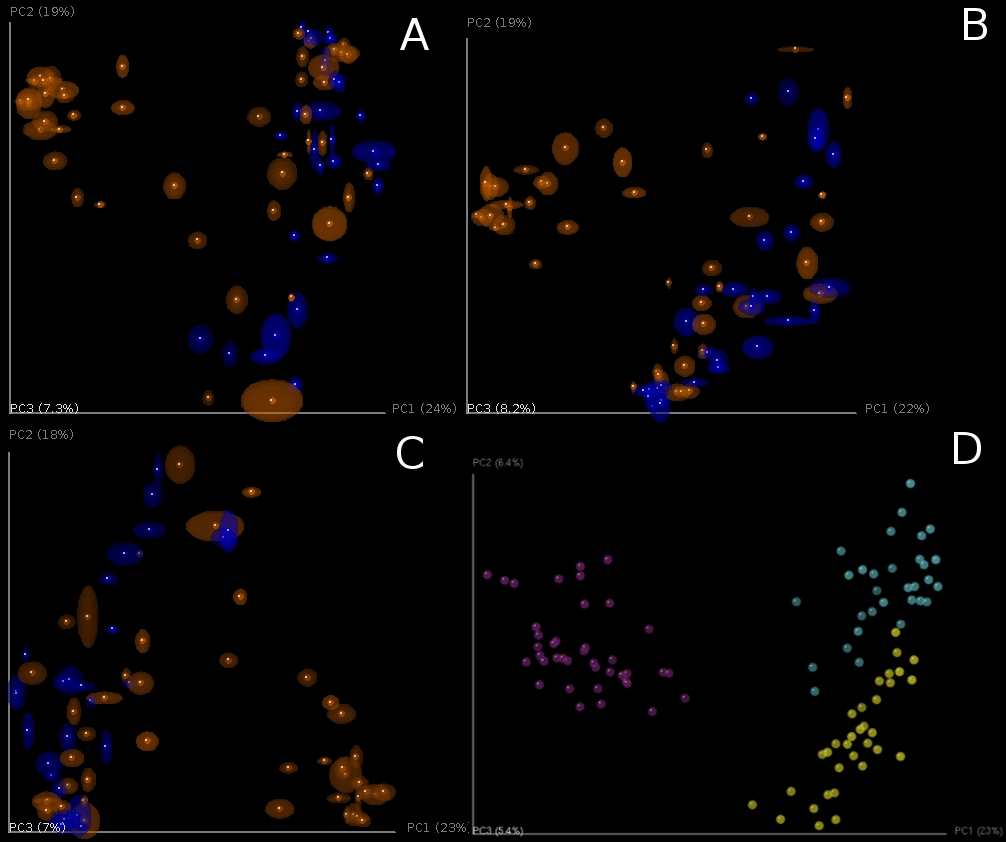
\includegraphics[width=0.75\columnwidth]{chapter_book_figures/Figure_7.jpg}
\caption[PCoA plots of unweighted Unifrac beta diversity]{\textbf{PCoA plots of unweighted Unifrac beta diversity.}
Panels A-C shows jackknifed replicate results for the example data set using de novo \gls{otu} picking,
closed-reference \gls{otu} picking and open-reference \gls{otu} picking, illustrating different results from the
three \gls{otu} picking approaches (Table ~\ref{btable3}). Each dot represents a sample, either from a WT
mouse (orange) or TG mouse (blue). The two groups are not clearly separated, probably because the
data set is contaminated (recall that this is a class project and different participants varied in
their dissection skills). The size of the ellipsoids show the variation for each sample calculated
from jackknife analysis. These plots are generated by the command jackknifed\_beta\_diversity.py
-i \$PWD/denovo\_otus/otu\_table\_filtered.biom -t \$PWD/denovo\_otus/rep\_set.tre -m \$PWD/IQ\_Bio\_16sV4\_L001\_map.txt
-o \$PWD/diversity\_analysis/jk\_denovo -e 7205 -a -O 64 (the input parameters should be adapted for using
the \gls{otu} tables from different \gls{otu} picking approaches). Panel D shows the beta diversity PCoA plot of a data set
from the “keyboard” data set \cite{Fierer2010} which links individuals to their computer keyboard through
microbial community similarity. Each dot represents a microbial community sampled from either fingertips or
keyboard keys from three individuals, annotated by the three colors shown in the plot. In contrast to panels A-C,
Panel D shows the microbial communities well-separated by individual in the PCoA plot.}
\label{bfigure7}
\end{figure}

Taxonomic information can be displayed on top of the PCoA using biplots (Figure ~\ref{bfigure8})
(this analysis requires the output file from previous taxon summary step). The coordinates
of a given taxon are computed as the weighted average of the coordinates of all samples,
where the weights are the relative abundances of the given taxon in the set of samples.
This plot is particularly suited for identifying taxa that drive the differentiation
between groups of microbial communities.

\begin{figure}[htbp]
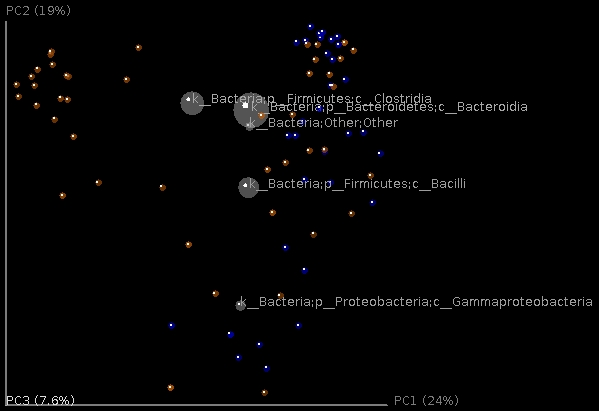
\includegraphics[width=0.75\columnwidth]{chapter_book_figures/Figure_8.jpg}
\caption[Biplot of the example data set]{\textbf{Biplot of the example data set.}
This is the unweighted Unifrac beta diversity plot, similar to Figure ~\ref{bfigure7},
with labels for the most 5 abundant phylum-level taxa added. The size of the sphere
for each taxon is proportional to the mean relative abundance of that taxon across all
samples. This plot is created by the command make\_3d\_plots.py -i
\$PWD/diversity\_analysis/open\_ref/bdiv\_even7205/unweighted\_unifrac\_pc.txt -m
\$PWD/IQ\_Bio\_16sV4\_L001\_map.txt -t
\$PWD/diversity\_analysis/open\_ref/taxa\_plots/table\_mc7205\_sorted\_L3.txt
--n\_taxa\_keep 5 -o \$PWD/diversity\_analysis/3d\_biplot}
\label{bfigure8}
\end{figure}

Another popular method for finding relationships among samples is hierarchical clustering,
which groups samples together into a tree. Although hierarchical clustering can be effective
in some cases, it should be used with caution because the eye can easily be drawn to incorrect
relationships (such as samples that are adjacent in terms of the order of their labels but are topologically
far apart in the tree). In general, we recommend using PCoA as a method of detecting grouping in the data,
but demonstrate hierarchical clustering here as an example. Here we analyze the beta diversity
distance matrix using UPGMA, which forces the samples into an ultrametric tree (i.e. a tree in
which the distance from the roots to the tips is the same for every tip) (Figure ~\ref{bfigure9}).
The resulting tree file is in Newick format, and can be visualized by programs including
TopiaryExplorer \cite{Pirrung2011}, the R package ape \cite{Paradis2004} and the package
distory \cite{Chakerian2012}. UPGMA can also be applied to the jackknifed subsamples to
provide an estimate of the statistical confidence in the clustering, by showing the
frequency of each nodes in the original full data set cluster that are supported by the
jackknife replicates. We generally recommend against the use of hierarchical clustering
as a method for identifying and visualizing sample groupings, so have not invested as
much effort in enabling this technique in \gls{qiime} as has been invested in other
visualizations. However, if you do plan to use hierarchical clustering, it is important
to be aware that substantial work has been done on more effective visualization
methods, e.g. in distory \cite{Chakerian2012}, and performing additional analyses
outside \gls{qiime} may allow improvements over the default visualizations.

\begin{figure}[htbp]
\includegraphics[width=0.75\columnwidth]{chapter_book_figures/Figure_9.jpg}
\caption[Bootstrapped UPGMA clustering on the example data set]{\textbf{Bootstrapped UPGMA clustering on the example data set.}
The tree is shown with the internal nodes colored by bootstrap support (red: 75-100\%,
yellow: 50-75\%, green: 25-50\% and blue: $<$ 25\%). Although this visualization
is popular in the literature, we generally recommend alternatives such as PCoA.}
\label{bfigure9}
\end{figure}

\textbf{Statistical significance of differences in alpha and beta diversity.} Which
statistical tests should be applied depends on the particular hypotheses and predictions
defined \emph{a priori} in a given research study. \gls{qiime} implements several scripts
that perform a broad range of statistical tests between samples or groups of samples
using both alpha and beta diversity measurements. For alpha diversity, the
compare\_alpha\_diversity.py script performs comparisons between groups of samples.
The script uses the alpha diversity measurements of samples standardized to a given number
of sequences per sample, and performs nonparametric two-sample t-tests (i.e. using Monte Carlo
permutations to calculate the p-value) comparing each pair of groups of samples.
Rarefaction is a critical step in these analyses, as noted above, because typically diversity
estimates depend on the number of sequences per sample. At the maximum rarefaction depth,
wild type and transgenic mice did not show differences in alpha diversity as measured by PD
metric (wild type: (mean +/- sd) = 45.19 +/- 10.6; transgenic: 40.01 +/- 9.5; t = -2.17, p = 0.102).
We also tested for differences in alpha diversity between body sites. We found differences
between cecum and ileum (cecum (mean +/- s.d.) = 51.1 +/- 3.6; ileum: 36.72 +/- 8.2; t = 5.35, p = 0.028),
cecum and mouth (mouth: 29.54 +/- 10.1; t = 6.62, p = 0.028) and feces and
mouth (feces: 48.4 +/- 4.0; t = 5.47, p = 0.028). None of the other pairs of comparisons
between body sites showed significant differences in alpha diversity (colon: 46.0 +/- 9.2;
multi-tissue: 46.26 +/- 9.1; skin: 42.13+/- 7.4; all p-values $>$ 0.056).

The appropriate statistical tests of beta diversity also depend on the research question
being asked. These tests compare sets of distances between samples in the distance matrix.
Careful attention must be paid both to Type I error (rejecting the null hypothesis when it is actually
true), and to Type II error (accepting the null hypothesis when it is actually false, i.e. lack of
statistical power). Type I error is more likely when variance is unequal between groups, and when
many comparisons are performed on the same data (although multiple comparisons corrections correct
for the increased Type I error, they often raise the Type II error rate instead). As always,
results should be interpreted with caution and common sense. A highly statistically significant
result stemming from data with a low correlation coefficient may indicate that a relationship
has little biological meaning, and examining the scatterplot to see if the result is driven by a
few outliers would be prudent. Further theoretical validation (especially of the multivariate
statistical tests) is also needed, especially because the distributions underlying microbial
community data have in general not yet been well characterized.

Comparisons between distance matrices are performed in \gls{qiime} using the
compare\_distance\_matrices.py script. This script can perform analyses including
the Mantel test, the Partial Mantel test, and the Mantel Correlogram. The Mantel
test is a non-parametric test that compares two distance matrices, and calculates
a correlation coefficient and a significant p-value using permutations that preserve
the rows and columns. For the purpose of showing some examples (because the mouse
data does not include a time series component), we will use the sequence dataset published
by Caporaso et al. \cite{Caporaso2011}, where the authors studied variation in the
bacterial community in the human gut over time series. We will compare the Unifrac
distance matrix and a distance matrix as differences in days since the treatment started.
Both distance matrices showed a significant correlation (Mantel test: p = 0.035),
showing that bacterial communities were more similar as they were close in sampling.
The Mantel test measures the overall correlation between distance matrices, but Mantel Correlograms
measure this effect when taking into account the distances between samples marked by specific
metadata variables. Essentially, the second distance matrix (in our case, days since the
treatment started) is divided into classes. The classes into which the second distance
matrix (days after experiment started) is determined by Sturge's rule, a method for
determining the width of bars in a histogram based on the binomial formula. Then Mantel
tests are run between these distance classes and the beta diversity distance matrix.
We found that none of the distance classes were significantly related to the bacterial
community (Figure ~\ref{bfigure10}: all comparisons p $>$ 0.120, after Bonferroni correction
for multiple comparisons). The Mantel test showed us that there is an overall correlation between
bacterial community and “days after the experiment started” (samples collected closer in
time had more similar bacterial communities), and Mantel Correlogram showed that there is
no significant correlation between the bacterial community and any of the classes into which
the “days after the experiment started” matrix was divided. In other words, in this
case, discretization of the data into a few timepoint classes led to an undetectable pattern;
in contrast, use of the whole time series yielded an interpretable result. However, in other
datasets, the reverse is often true, especially if the variation is not monotonic
(e.g. in the case of seasonal variation).

\begin{figure}[htbp]
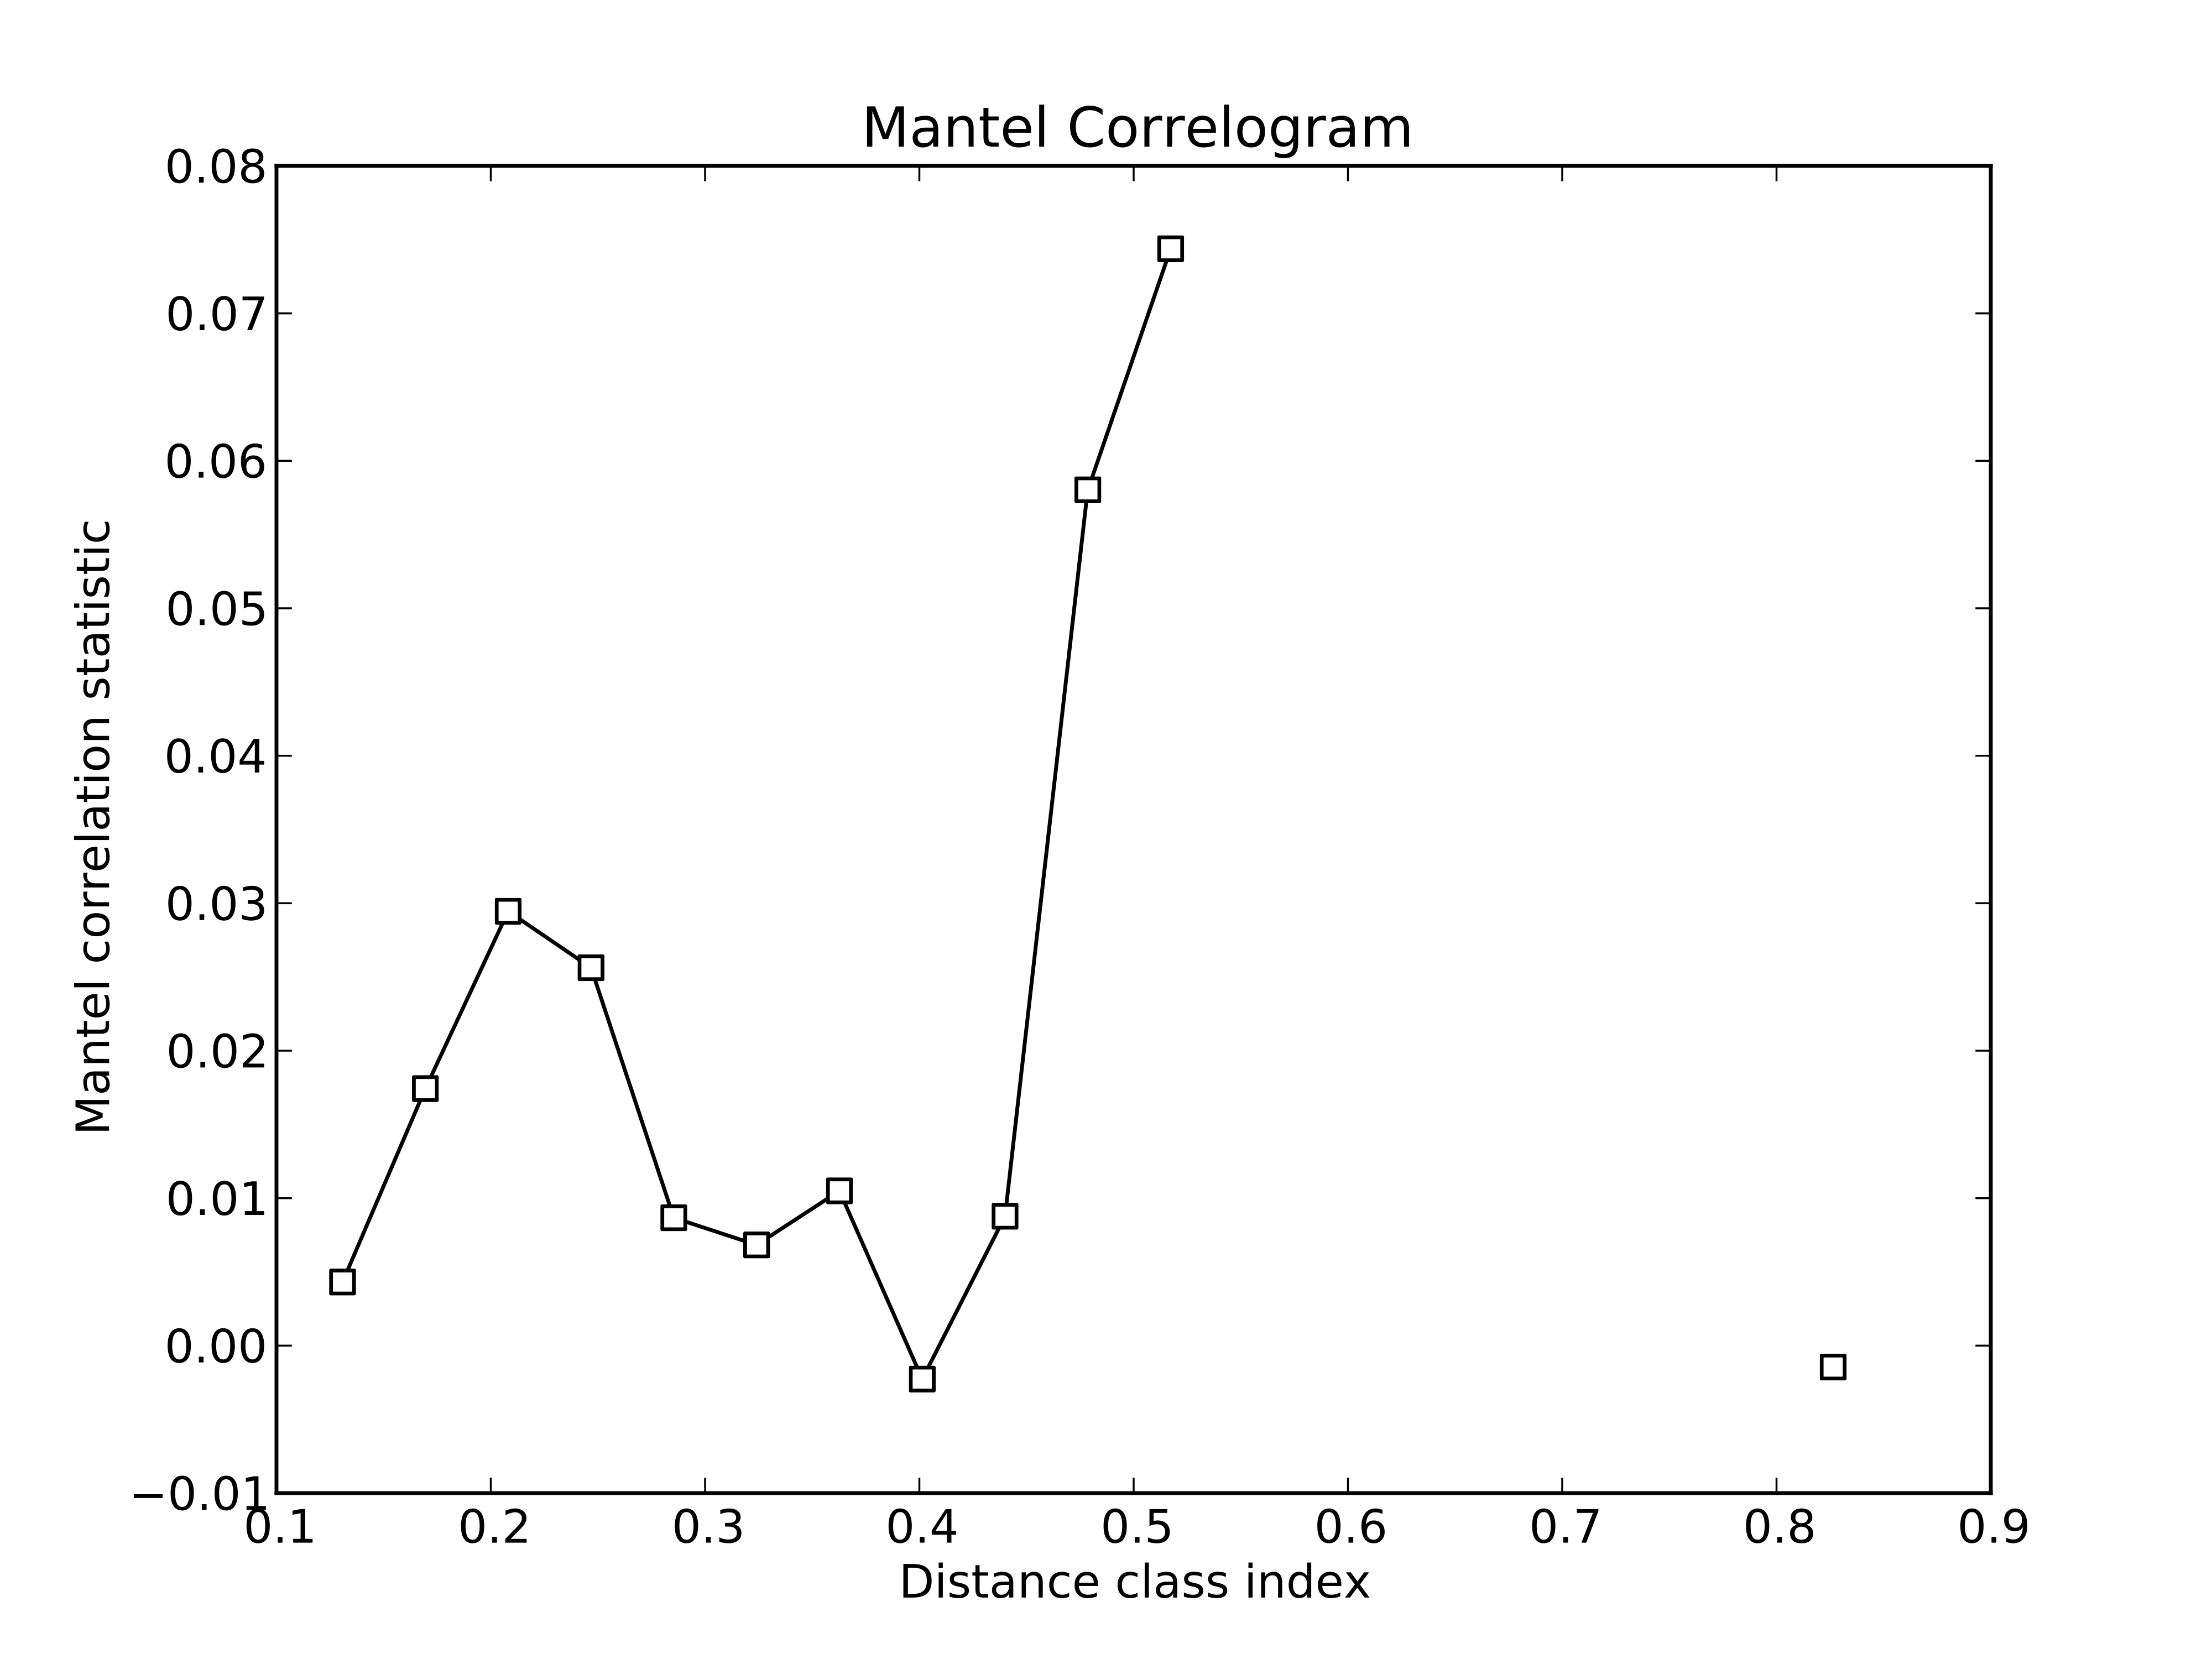
\includegraphics[width=0.75\columnwidth]{chapter_book_figures/Figure_10.jpg}
\caption[Mantel Correlogram showing the Mantel correlation statistics between unweighted Unifrac distance matrix and each class in the days after experiment started distance matrix]{\textbf{Mantel Correlogram showing the Mantel correlation statistics between unweighted Unifrac distance matrix and each class in the days after experiment started distance matrix.}
Classes in the second distance matrix are determined by Sturge's rule. White dots show non-significant relationship since black dots show significant ones.}
\label{bfigure10}
\end{figure}

The partial Mantel test is similar to the Mantel test, except that the analysis is
controlled by a third variable. When we compare the beta diversity distance matrix
with days after the experiment started by controlling by sampling date, we find the
same trend noted before (Partial Mantel test: p = 0.010). Samples collected
close in time have similar bacterial communities and this effect is independent of the date of collection.

Several visual and statistical tests have been implemented in \gls{qiime} in order to compare
between and within beta-diversity distances. Distance histograms are an easy way to
compare both types of distances graphically (make\_distance\_histograms.py). The output
is an html file that shows as many histograms as categories. It is very useful to compare
all-within “category” against all-between “category”, or the distribution of distances
within each group (Figure ~\ref{bfigure11}). Probably a more useful tool to compare these
beta-diversity distances is by means of box-plots (make\_distance\_boxplots.py, Figure ~\ref{bfigure12}).
The box-plot script generates a box-plot graph and performs a t-test. Box-plots showed that
there were no differences between the distances within mouse type and between types.
However, the statistical test shows highly significant differences (p $<$ 0.001) when comparing
within and between distances. Once again, we recommend caution and common sense when the
p-values are interpreted. It is likely to get a significant p-value, although a close
inspection of the box-plot reveals that standard error bars overlap. Basically this
result is due to the large number of comparisons: a small Student t-statistic
(obtained when differences between two data set are small) and these large degrees
of freedom may be highly significant (i.e. the two data set are very different) even
with conservative multiple test corrections (as Bonferroni).

\begin{figure}[htbp]
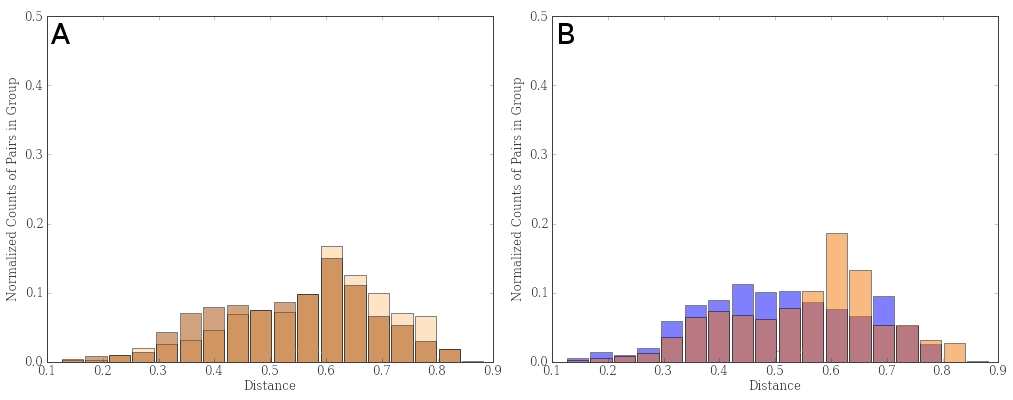
\includegraphics[width=\columnwidth]{chapter_book_figures/Figure_11.jpg}
\caption[Histograms of the example data set]{\textbf{Histograms of the example data set.}
(A) Histogram showing distribution of distances between (light brown) and within
(dark brown) mice gut microbiota taking into account both wild type and transgenic
mouse groups. (B) Distribution of within distances in gut bacterial community of wild
type mice (light orange) and transgenic ones (blue).}
\label{bfigure11}
\end{figure}

\begin{figure}[htbp]
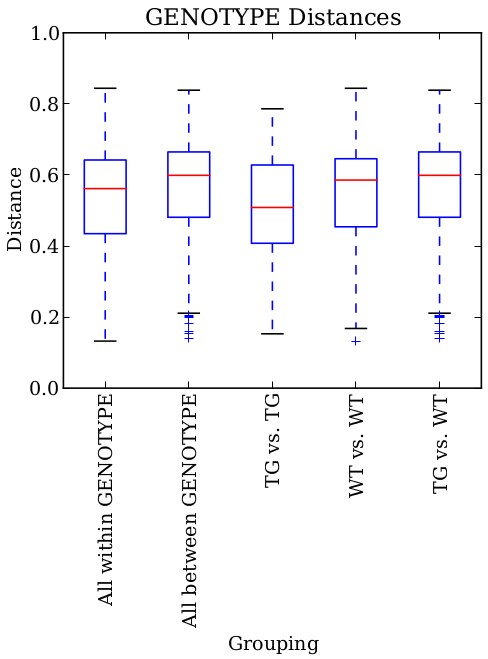
\includegraphics[width=0.75\columnwidth]{chapter_book_figures/Figure_12.jpg}
\caption[Box-plots of the unweighted UniFrac distances for bacterial gut microbiota in both mouse type (WT: wild type; TG: transgenic)]{\textbf{Box-plots of the unweighted UniFrac distances for bacterial gut microbiota in both mouse type (WT: wild type; TG: transgenic).}
“Within” distances represent distances within any of the two groups since “between” distances
show distances between both groups. “TG vs. TG” and “WT vs. WT” represent within distances in
transgenic and wild type groups respectively. Although averages are different, standard error overlaps
in all cases.}
\label{bfigure12}
\end{figure}

Other multivariate analyses provide additional powerful tools for exploring significant
relationships between the beta diversity distance matrix and factors or covariates.
compare\_categories.py offer different statistical tests, where ANOSIM and adonis are
usually employed. ANOSIM is a non-parametric statistical test that compares ranked
beta-diversity distances between different groups and calculates a p-value and a correlation
coefficient by permutation. Adonis partitions the variance in a similar way to the
ANOVA family of tests, specifically testing variation within a category is smaller
or greater than variation between categories. It calculates a pseudo F-value, a
p-value and a correlation coefficient (R2). Significant p-values must be
interpreted together with their R2 values to infer biological meanings from the results.
It is worth to mentioning here that PERMANOVA and adonis are similar statistical methods,
and usually provide equivalent results. However, PERMANOVA only allows categorical factors,
whereas both categorical and continuous variables may be used in adonis. Both ANOSIM and
adonis analyses indicate that bacterial communities in wild-type and transgenic mice
significantly differ from one another (ANOSIM: r = 0.134, p $<$ 0.001; adonis, r2 = 0.046, p $<$ 0.001).
However, the correlation coefficients are low, so the significant p-values need to be
interpreted cautiously because this result may not be biologically relevant.


\textbf{\gls{otu} networks.} Network-based analysis can sometimes be very useful for
displaying how \gls{otu}s are partitioned between samples, and how samples are related
each other, although we have found that this analysis only works well for datasets
in which the samples are not all equally connected. Networks are therefore a powerful
way for visually displaying certain large and complex datasets to emphasize similarities
and differences among samples. Network analyses are implemented in \gls{qiime} through the
script make\_otu\_network.py. This script generates the \gls{otu} network files to be
passed into Cytoscape \cite{Shannon2003} and statistics for those networks (specifically,
a bipartite graph in which nodes represent either \gls{otu}s or samples, and edges represent
a connection between an \gls{otu} and a sample (Ley et al., 2008)). Cytoscape is not wrapped
in the \gls{qiime} pipeline and it is run as a separate program. The files used by Cytoscape 2.8.2 are:
the real edge table (real\_edge\_table.txt) which contains the columns “from”, “to”, “eweight” and
“consensus\_lin”, among others dictated by the headers in the mapping file; and the real
node file (real\_node\_table.txt) which contains a node for each \gls{otu} and each sample in
the study. It uses the \gls{otu} file and the user metadata mapping file.

The visual output of this analysis is a clustering of samples according to their shared \gls{otu}s
(i.e. samples that share more \gls{otu}s cluster closer together, as do \gls{otu}s shared by more samples):
samples and \gls{otu}s are represented as dots in the space (“nodes”) and connected by lines (“edges”).
The degree to which samples cluster is based on the number of \gls{otu}s shared between samples, and this
is weighted according to the number of sequences within an \gls{otu}.

In the network diagram, both types of nodes, \gls{otu} nodes and sample nodes, can be
easily modified using Cytoscape's graphical user interface, with symbols such as
filled circles for \gls{otu}s and filled squares for samples. If an \gls{otu} is found within a
sample, both nodes are connected with a line (an edge). The nodes and edges can then
be colored to emphasize certain aspects of the data.

This method is not simply used for descriptive visualizations: the connections within
the network can also be analyzed statistically to provide support for the clustering patterns
displayed in the network. A G-test for independence is used to test whether sample nodes within
categories (such as within a genotype, in our example mouse study) are more connected within
than a group than expected by chance. Each pair of samples is classified according to whether
its members shared at least one \gls{otu}, and whether they share a category. Pairs are then
tested for independence in these categories (this asks whether pairs that share a category
also are equally likely to share an \gls{otu}). This statistical test can also provide support
for an apparent lack of clustering when it appears that a parameter is not contributing
to the clustering.

In our example dataset, mouse samples show some degree of clustering in the space
depending on whether the genotype is wild-type or transgenic (Figure ~\ref{bfigure13}).
These clusters in the network were significant different (G-test: p $<$ 0.001). Surprisingly,
bacterial communities of mice did not visually cluster by body site, although the statistical
test shows highly significant differences in samples from different body sites. These results
must be interpreted cautiously. The degrees of freedom in the statistical test depend on the
number of comparisons so, highly significant results might be obtained even when differences
between clusters are slight. In other cases, these differences are obvious and easy to interpret.
In the first application of this analysis in microbial ecology, the gut bacteria of a variety of
mammals was surveyed, and the network diagrams were colored according to the diets of the animals,
which highlighted the clustering of hosts by diet category (herbivores, carnivores, omnivores). In a
later meta-analysis of bacterial surveys across habitat types, the networks were colored in such a
way that the phylogenetic classification of the \gls{otu}s was highlighted: this analysis revealed
the dominance of shared Firmicutes in vertebrate gut samples versus a much higher diversity of
phyla represented amongst \gls{otu}s shared among environmental samples \cite{Ley2008}.

\begin{figure}[htbp]
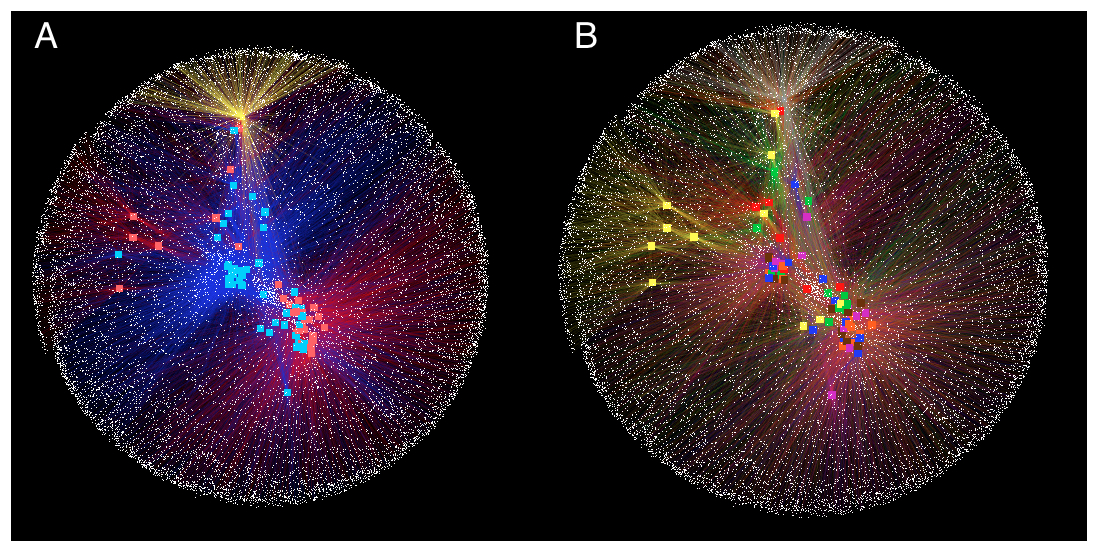
\includegraphics[width=\columnwidth]{chapter_book_figures/Figure_13.jpg}
\caption[\gls{otu}-Network bacterial community analysis applied in wild type and transgenic mice]{\textbf{\gls{otu}-Network bacterial community analysis applied in wild type and transgenic mice.}
(A) Network colored by genotype (wild type: blue; transgenic: red). Control sample (yellow dot) is
external in the network and several \gls{otu} are not shared with mice. Although we can see some degree of
clustering, discrimination by genotypes is difficult to assess. (B) Network colored by body site
(mouth: yellow; skin: in red; ileum: in blue; colon: in pink; cecum: in orange; feces: in brown;
and multi-tissue samples: in green). A control sample is colored in grey. There is no clear sample
clustering by body site, suggesting that there is not a core set of \gls{otu}s that differentiates one site from another.}
\label{bfigure13}
\end{figure}

This \gls{otu}-based approach to comparisons between samples provides a counterpoint to the
tree-based PCoA graphs derived from the UniFrac analyses. In most studies, the two
approaches reveal the same patterns. They can, however, reveal different aspects of the
data. The network analysis can provide taxonomic connections among samples in a visual manner,
whereas PCoA-UniFrac clustering can reveal sub-clusters that may be obscured in the network.
The principal coordinates can be pulled out individually and regressed against other metadata;
the network analysis can provide a visual display of shared versus unique \gls{otu}s. Thus, together
these tools can be used to draw attention to different aspects of a dataset.

\textbf{\gls{otu} heatmaps.} Another method to visualize the relationships between \gls{otu}s
and samples is the heatmap, which is widely used for other applications in molecular
biology \cite{Wilkinson2009}. This method was initially developed by Loua \cite{Loua1873}
to visualize population characteristics of 20 districts of Paris.

In our case, heatmaps can be used for exploratory analysis of microbiomes by mapping
abundance values to a color scale in a condensed, pattern-rich format, in which each
row corresponds to an \gls{otu} and each column corresponds to a sample. A good heatmap
graphic can generate hypotheses about sample and/or \gls{otu} clustering in the data, which can
then be followed up with additional more formal analyses. Two key structural aspects of a
heatmap graphic greatly affect whether it will reveal interpretable patterns: (1) the ordering
of the axes, and (2) the color scaling.

\gls{qiime} can create \gls{otu} heatmaps using two different scripts: make\_otu\_heatmap.py and
make\_otu\_heatmap\_html.py. The first script generates a heatmap in which \gls{otu}s are
represented in rows and samples in columns. \gls{otu}s and samples can be sorted and clustered
by the phylogenetic tree and by the UPGMA hierarchical clustering, respectively. However,
the visualizations of both trees (phylogenetic and hierarchical) in the final heatmap
are not currently implemented directly in \gls{qiime}, and these hierarchical displays must be
prepared using external software such as R. \gls{qiime} also supports sample clustering by a metadata
category if the user provides a mapping file. The samples will be clustered within each category
level using Euclidean UPGMA. The script sort\_otu\_table.py allows sorting the \gls{otu} table by a
category in the mapping file, allowing defining the order of the samples in the heatmap.
Figure ~\ref{bfigure14} shows the output of make\_otu\_heatmap.py. There we can see a drawback
to heatmaps: when the number of samples or \gls{otu}s included in the graphic is too high, the density
of the graphic can be overwhelming. Thus, we recommend that the \gls{otu} table be filtered to a
smaller number of samples (or categories) and taxa to identify the most important patterns,
as we will show later in this section.

\begin{figure}[htbp]
\includegraphics[width=0.75\columnwidth]{chapter_book_figures/Figure_14.jpg}
\caption[Heatmap of \gls{otu}s present in the different samples from transgenic and wild type mice]{\textbf{Heatmap of \gls{otu}s present in the different samples from transgenic and wild type mice.}
The intensity of black shows the abundance of certain \gls{otu} in each sample.
Both samples and \gls{otu}s are sorted by UPGMA tree and the \gls{otu} phylogenetic tree, respectively.}
\label{bfigure14}
\end{figure}

The second script (make\_otu\_heatmap\_html.py) creates an interactive \gls{otu} heatmap
from an \gls{otu} table (Figure ~\ref{bfigure15}). This script parses the \gls{otu} count table
and filters the table by counts per \gls{otu} (user-specified). It then converts the table
into a javascript array, which can be loaded into a web browser. The \gls{otu} heatmap
displays raw \gls{otu} counts per sample, where the counts are colored based on the
contribution of each \gls{otu} to the total \gls{otu} count present in the sample (blue:
contributes low percentage of \gls{otu}s to sample; red: contributes high percentage of
\gls{otu}s). This web application allows the user to filter the \gls{otu} table by number of
counts per \gls{otu}. The user also has the ability to view the table based on taxonomy
assignment. Additional features include: the ability to drag rows up and down by
clicking and dragging on the row headers; and the ability to zoom in on parts of
the heatmap by clicking on the counts within the heatmap.

\begin{figure}[htbp]
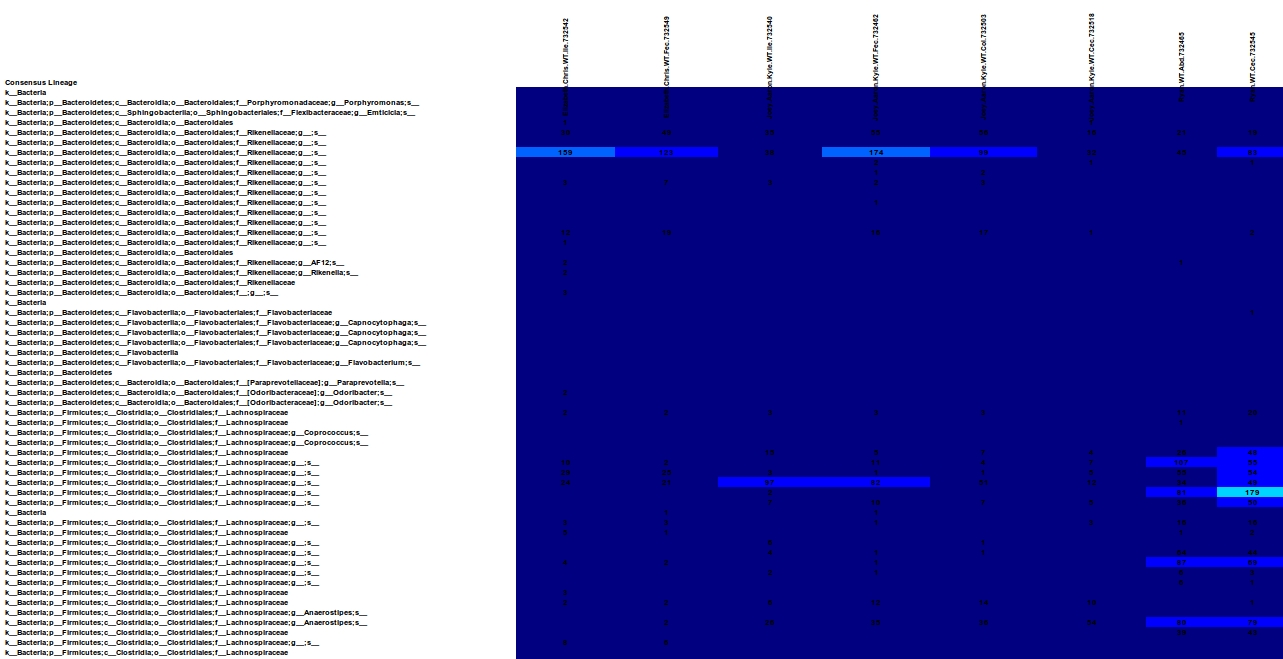
\includegraphics[width=0.75\columnwidth]{chapter_book_figures/Figure_15.jpg}
\caption[Interactive heatmap of \gls{otu}s present in the different samples from transgenic and wild type mice]{\textbf{Interactive heatmap of \gls{otu}s present in the different samples from transgenic and wild type mice.}
This visualization is a result of an HTML file that can be opened in any web browser.
The advantage of this heatmap is that it is easy to manipulate the abundance level for
coloring, or transpose samples and \gls{otu}s between columns and rows.}
\label{bfigure15}
\end{figure}

Improved \gls{otu} heatmap visualizations can be generated using the plot\_heatmap() command
in the phyloseq package for R \cite{McMurdie2013}. This package takes a similar approach
to NeatMap \cite{Rajaram2010}, in that it uses ordination results rather than hierarchical
clustering to determine the index order of each axis. For plot\_heatmap, the default color
scaling maps a particular shade of blue to a log transformation of abundance that generally
works well for microbiome data, although the user can select alternative transformations.

In this example, a key step was proper filtering of the data. We removed \gls{otu}s that appear in only a
few samples. The possible contribution to the graphic of these infrequent \gls{otu}s is limited, more often
contributing to “noise” that causes the heatmap to look dark, empty, and uninterpretable (see Figure ~\ref{bfigure14}).
We used a non-metric multidimensional scaling of the Bray-Curtis distance to determine the order of the \gls{otu}s and
samples. From this representation, it is possible to distinguish high-level patterns and simultaneously note the
samples and \gls{otu}s involved. For instance, all but a few of the mouth samples are in a cluster toward the middle of the
heatmap. One of the key features of this group is an obvious relative overabundance of three Firmicutes \gls{otu}s, which
are among the most abundant in this subset of the data. Similarly, another clear pattern is a distinction between a
group of wild type samples from various body sites on the left of the heatmap that appear to have higher proportions
of a number of different Firmicutes \gls{otu}s, as well as a few specific Bacteroidetes \gls{otu}s. This is distinct from the
largest cluster of samples on the right-hand side of the heatmap, in which many of the most-abundant \gls{otu}s are a
different subset of Bacteroidetes and Firmicutes \gls{otu}s. We also found it helpful to further pursue these high-level
patterns by splitting the data into Firmicutes-only and Bacteroidetes-only subsets, and then plotting new heatmaps
with finer-scale taxonomic labels. This required essentially the same commands and limited additional effort, well-tailored
for exploratory interactive analysis, much of which we have documented in Supplemental File 1.

Although heatmaps have been deployed widely in molecular biology, especially in protein expression studies, some of the
other displays we have discussed such as principal coordinates plots and taxonomy plots often provide more easily
interpretable results. However, summarizing relations between taxa through ordination plots or network analyses
have been shown to be powerful tools for highlighting similarities and differences among samples and taxa in our
\gls{otu} table, and a carefully constructed heatmap (though not, in most cases, the default output) can be a useful
guide to understanding and hypothesis generation.

\textbf{\gls{otu} category significance.} The experimental design of a microbial study will often involve
comparing two or more groups for differences in the abundance of \gls{otu}s; for example, are there taxa
that significantly differ between the control group and the experimental group? One way to assess
this question is to compare the relative abundances of each microbial member between the two groups.
This functionality is built into a script called otu\_category\_significance.py. We can test if there
are significant differences in \gls{otu} abundance between mouse genotypes either wild type (WT) or transgenic
(TG). We can assess differences between these groups using the following command:

\begin{lstlisting}[language=bash]
otu_category_significance.py \
 -i $PWD/diversity_analysis/open_ref/table_mc7205.biom \
 -m $PWD/IQ_Bio_16sV4_L001_map.txt \
 -o $PWD/open_ref_otu_categ_sig_output -c GENOTYPE \
 -s ANOVA
\end{lstlisting}

Here we run an ANOVA to assess the relative abundance of each taxon in the \gls{otu} table between our
two genotype groups. The output will be written to a user-specified file called otu\_cat\_sig.txt.
This document will list the \gls{otu} ID, the raw p-value, the Bonferonni corrected p-value, the False
Discovery Rate (FDR) p-value, as well as the relative average abundance for each of the groups in
the selected category (genotype in our case), and the \gls{otu} taxonomy string (if provided in the initial
\gls{otu} table). While many of these taxa may be significantly different between groups according to the
raw p-value, it is extremely important that only p-values that have been corrected for against multiple
comparisons, using either Bonferroni or FDR, be considered as significant. Many times a user's \gls{otu}
table will contain hundreds or thousands of \gls{otu}s, and thus a p-value is likely to reach significance
based solely on the large number of statistical comparisons being computed (for a probability threshold
of 0.05, 1 of 20 comparisons results significant just by chance). It is often very helpful to open the
.txt files produced by otu\_category\_significance.py in a spreadsheet so that columns can be sorted
according to p-values.

The otu\_category\_significance.py script also contains several other statistics for comparing groups.
The g-test can be used to determine if the presence or absence of a given taxa is significantly different
between groups, and can be specified by passing the option -s g\_test in the command. The user can also
run a paired t-test to determine whether there are taxa that significantly differ between two paired points.
For example, imagine the experimental design sampled a group of mice before and after a dietary intervention.
Using the paired-t statistic in otu\_category\_significance.py would then compare each mouse's after timepoint
to the before timepoint, and test for differences that were consistent across mice, rather than grouping all
the before and after timepoints together. For continuous variables, \gls{qiime} can calculate the Pearson correlations
of \gls{otu} abundance with those variables. \gls{qiime} is also capable of longitudinal data analysis, which is suitable
for the samples tracking the same subjects at multiple points in time, e.g., the oral microbiota of 6 persons
after meals in a day. Specifically, longitudinal Pearson correlation can be calculated, accounting for intra-subject
correlation of measurements.

\textbf{Machine learning.} \gls{qiime} can also take advantage of several machine learning algorithms to solve
two important issues in high-throughput metagenomic studies: correction of mislabeling, and quantifying
sample contamination.

This mislabeling problem is an increasing issue as the number of processed and pooled sequences
increases \cite{Knights2011Mislabel}. This mislabeling can be addressed using supervised classifiers,
a machine learning technique that is able to fix incorrect metadata. \gls{qiime} uses the random forest \cite{Breiman2001}
supervised classifier implemented in R \cite{Liaw2002} to recover the mislabeled samples by training the
classifier with the relative abundance taxa \cite{Knights2011SupClass}. Knights et al. \cite{Knights2011Mislabel}
shows that this approach can even recover up to 30-40\% mislabeled samples when the biological patterns are especially clear.

This same technique can be also applied to find taxa that play a key role in differentiating groups of samples, as
is done in \gls{otu} category significance. However, the difference between \gls{otu} category significance and the machine
learning technique is the type of model the construct. While the \gls{otu} category significance creates an explanatory
model (i.e. it gives a model that best fits the current dataset), the machine learning technique creates a predictive
model \cite{Knights2011SupClass}.That is, it creates a model that is able to generalize future data, minimizing the
expected prediction error.

Since the supervised learning trains a classifier, it is important to provide useful predictors (\gls{otu}s in our case).
Thus, it is highly recommended to filter the input \gls{otu} table to remove those \gls{otu}s that are present in few samples
(e.g. $<$ 10 samples). As in previous analyses, a rarified \gls{otu} table should be used, so that artificial diversity
induced due to different sampling effort is removed. In our example dataset, we can use the subsampled \gls{otu} table
generated for previous analyses and remove the low-abundance \gls{otu}s:

\begin{lstlisting}[language=bash]
filter_otus_from_otu_table.py \
 -i $PWD/diversity_analysis/open_ref/table_mc7205.biom \
 -o $PWD/diversity_analysis/open_ref/\
    otu_table_filtered10.biom \
 -s 10
\end{lstlisting}

Running the following command, will run the supervised learning algorithm using the GENOTYPE
category and 10-fold cross-validation, providing mean and standard deviation of errors:

\begin{lstlisting}[language=bash]
supervised_learning.py \
 -i $PWD/diversity_analysis/open_ref/\
    otu_table_filtered10.biom \
 -m $PWD/IQ_Bio_16sV4_L001_map.txt -c GENOTYPE \
 -o $PWD/open_ref_supervised_learning_output -e cv10
\end{lstlisting}

This script will store several files on the output folder. The most important file is summary.txt:

\begin{lstlisting}[language=bash]
cat $PWD/open_ref_supervised_learning_output/summary.txt
Model Random Forest
Error type 10-fold cross validation
Estimated error (mean +/- s.d.) 0.23373 +/- 0.15058
Baseline error (for random guessing) 0.42308
Ratio baseline error to observed error 1.81011
Number of trees 500
\end{lstlisting}

The important information in this file is the Ratio baseline error to observed error, which shows the
ratio between the expected error of the random forest classifier and the expected error of a classifier
that always guesses the most abundant class (Baseline error). Our recommendation is that a ratio of at
least 2 shows a good classification. In our example data set, this value is 1.81011, which is close to 2
but not enough to be considered a good classification.

The contamination quantification problem is addressed in \gls{qiime} using SourceTracker \cite{Knights2011}. Given a
list of known source environments and a sink (or set of sinks) environment(s), SourceTracker uses a Bayesian
approach jointly with Gibbs sampling to predict the quantity of taxa that each source, or an unknown source,
contributes to the taxa that makes up the sink environment. For a more detailed description of the algorithm,
see Knights et al. \cite{Knights2011}.

The first step to use SourceTracker in \gls{qiime} is to modify the mapping file of our example dataset and add two
columns: SourceSink and Env. The SourceSink column tells SourceTracker which sample is a source and which
sample is a sink, while the Env column provides the environment. In our example, we have defined samples from
mouth, ileum, cecum, colon, fecal pellet and skin as sources and the whole mouse homogenization as a sink. In
the Env column we have defined the environments as the body site (mouth, ileum, cecum, colon, feces, skin and homogenization).

As a machine learning algorithm, SourceTracker needs useful \gls{otu}s (predictors) as inputs for training the algorithm.
Here, we will use the same \gls{otu} table as used for the supervised\_learning.py script. However, SourceTracker does not
yet accept BIOM tables, so we have to transform them into to a tab-delimited \gls{otu} table (note that this table can also
be opened in Excel or other popular tools):

\begin{lstlisting}[language=bash]
convert_biom.py \
 -i $PWD/diversity_analysis/open_ref/\
    otu_table_filtered10.biom \
 -o $PWD/diversity_analysis/open_ref/\
    otu_table_filtered10.txt -b
\end{lstlisting}

Then, we \hspace{0.01cm} can \hspace{0.01cm} call \hspace{0.01cm} SourceTracker \hspace{0.01cm} using \hspace{0.01cm} the following
command (the \$SOURCETRACKER\_PATH variable should be defined if
you have successfully install SourceTracker):

\begin{lstlisting}[language=bash]
R --slave --vanilla --args \
 -i $PWD/diversity_analysis/open_ref/\
    otu_table_filtered10.txt \
 -m $PWD/IQ_Bio_16sV4_L001_map_ST.txt \
 -o $PWD/open_ref_sourcetracker_output \
 < $SOURCETRACKER_PATH/sourcetracker_for_qiime.r
\end{lstlisting}

The output from the SourceTracker algorithm is a set of pdf files that shows the mixture of
the sources that makes up the sink (see Figure ~\ref{bfigure17}).

\begin{figure}[htbp]
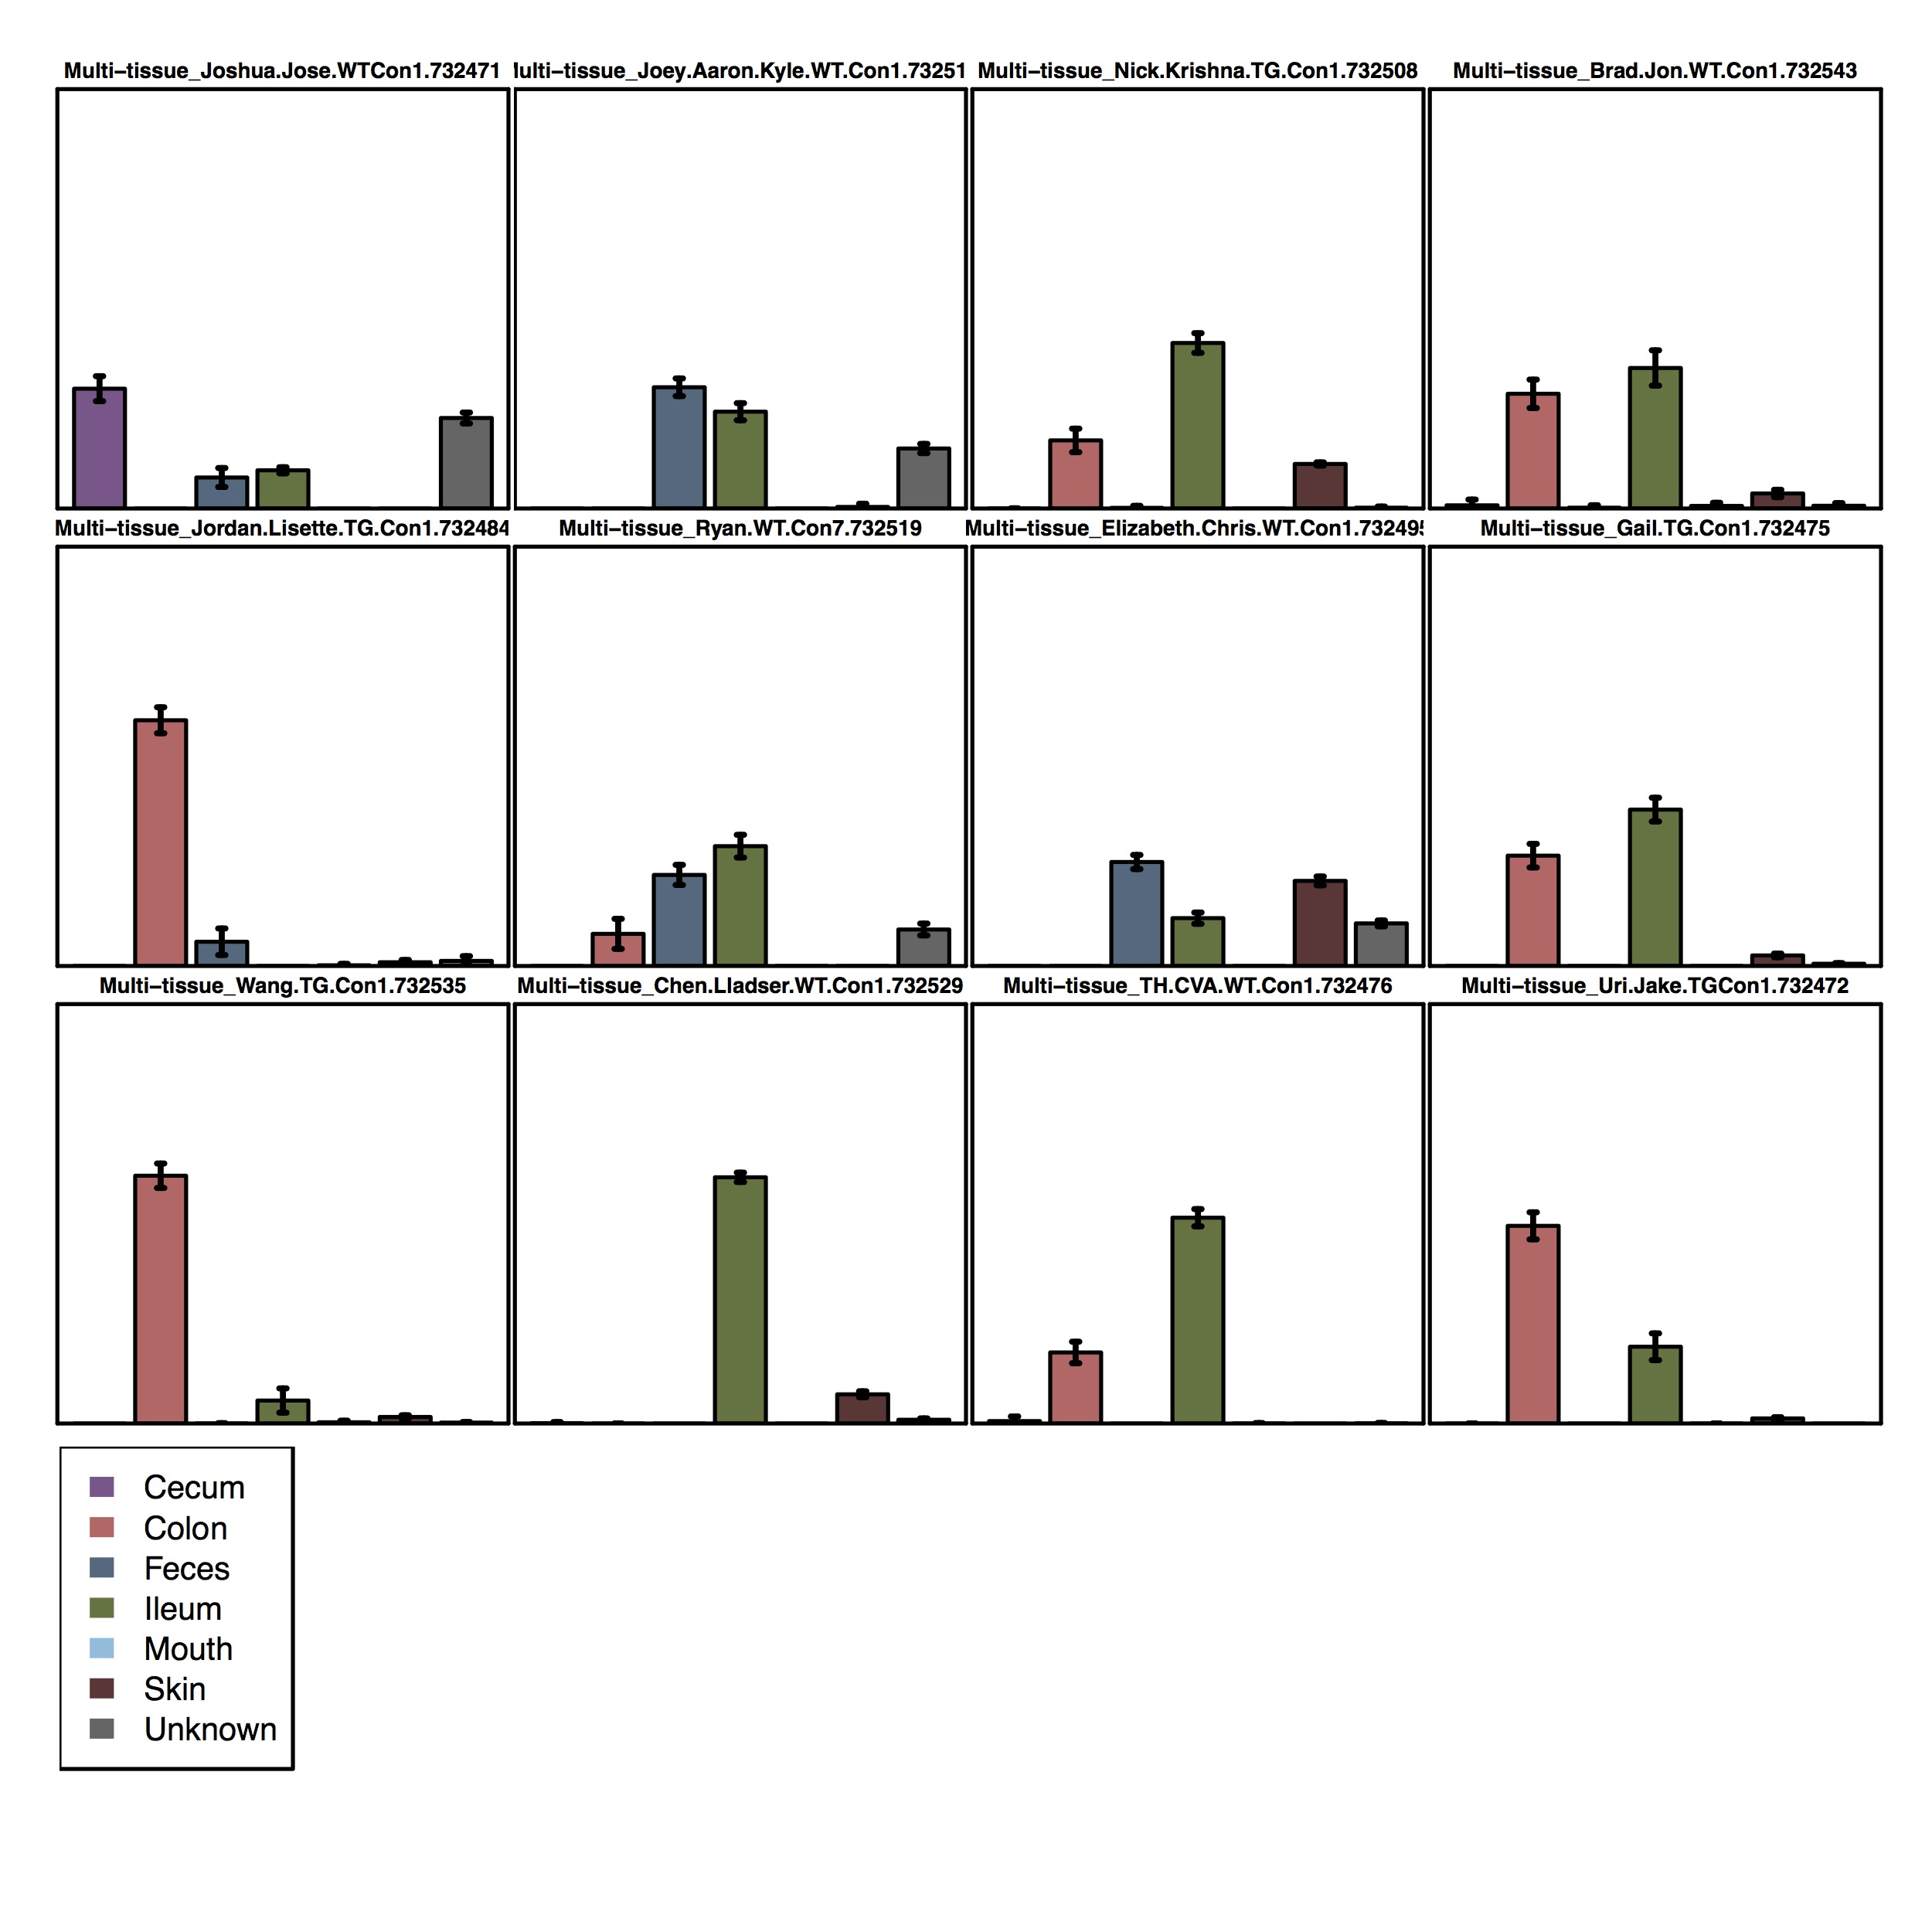
\includegraphics[width=\columnwidth]{chapter_book_figures/Figure_17.jpg}
\caption[SourceTracker output showing a bar plot for each sink (mouse) present in the dataset]{\textbf{SourceTracker output showing a bar plot for each sink (mouse) present in the dataset.}
Each bar is a potential source (body site) and the height of each bar represents the percentage of
taxa the source contributes to the taxa in the sink. The advantage of this visualization over the other
two (area and pie chart) is that it shows error bars that allow to see the variance of the prediction.}
\label{bfigure17}
\end{figure}

\textbf{Procrustes analysis.} When we want to compare samples in PCoA space that
were processed in different ways, such as: different ribosomal RNA subunits, primer sets,
or algorithmic choices for processing, we can use Procrustes analysis \cite{Gower1966, Muegge2011, Vinten2011}.
Procrustes analysis is a statistical shape algorithm that allows us to compare different distributions by
rescaling and applying a rotation matrix; this is, if the group of samples we are have the same shape but
in different size or orientation the algorithm will resize and rotate them to make the shapes fit. As an example,
we present the results of comparing the different \gls{otu} picking algorithms, where we can see that even as the number
of \gls{otu} clusters change the distribution described is similar with a confidence of MC p-value: 0.00 and M2: 0.097 for
closed-reference vs. de novo, and MC p-value: 0.00 and M2: 0.035 for closed-reference vs. open reference.
Both cases used the first three axes (i.e. the axes displayed in the plot), and 100 repetitions, Figure \ref{bfigure18}.
To generate these plots we ran these commands:

\begin{lstlisting}[language=bash]
transform_coordinate_matrices.py \
 -i $PWD/diversity_analysis/closed_ref/bdiv_even7205/\
 unweighted_unifrac_pc.txt,$PWD/diversity_analysis/denovo/\
 bdiv_even7205/unweighted_unifrac_pc.txt \
 -r 100 -o $PWD/procrustes/closed_ref-denovo

compare_3d_plots.py \
 -i $PWD/procrustes/closed_ref-denovo/pc1_transformed.txt,\
 $PWD/procrustes/closed_ref-denovo/pc2_transformed.txt \
 -o $PWD/procrustes/closed_ref-denovo/plot \
 -m $PWD/IQ_Bio_16sV4_L001_map.txt

transform_coordinate_matrices.py \
 -i $PWD/diversity_analysis/closed_ref/bdiv_even7205/\
 unweighted_unifrac_pc.txt,$PWD/diversity_analysis/\
 open_ref/bdiv_even7205/unweighted_unifrac_pc.txt \
 -r 100 -o $PWD/procrustes/closed_ref-open_ref

compare_3d_plots.py \
 -i $PWD/procrustes/closed_ref-open_ref/\
 pc1_transformed.txt,\
 $PWD/procrustes/closed_ref-open_ref/\
 pc2_transformed.txt \
 -o $PWD/procrustes/closed_ref-open_ref/plot \
 -m $PWD/IQ_Bio_16sV4_L001_map.txt
\end{lstlisting}

\begin{figure}[htbp]
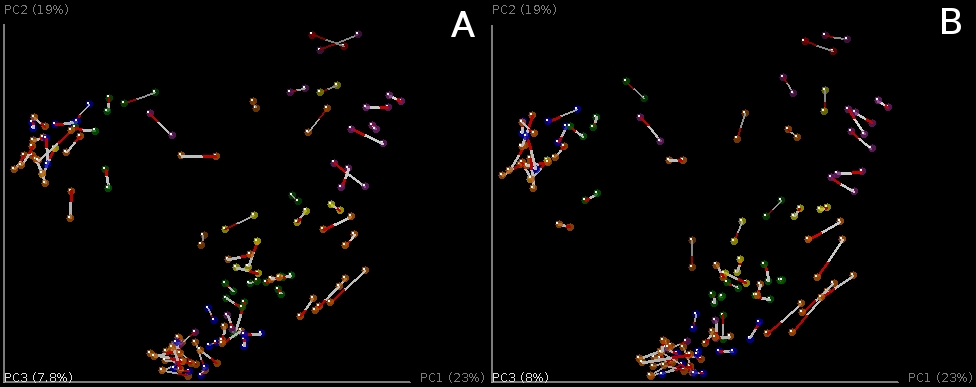
\includegraphics[width=\columnwidth]{chapter_book_figures/Figure_18.jpg}
\caption[Procrustes analysis of different picking algorithms, where we can see that different \gls{otu} clustering methods yield similar PCoA distributions]{\textbf{Procrustes analysis of different picking algorithms, where we can see that different \gls{otu} clustering methods yield similar PCoA distributions.}
PCoA plots are colored by BODY\_HABITAT. A) Comparing samples with clusters picked
using the de novo picking protocol against the closed-reference. B) Comparing
samples with clusters picked using the open-reference picking protocol against the closed-reference.}
\label{bfigure18}
\end{figure}

\textbf{SitePainter.} Spatial data poses unique challenges, and the types of statistical analyses
described above often obscure spatial patterns \cite{Gevers2012, Hewitt2013}.
SitePainter \cite{Gonzalez2012SitePainter} is a web-based tool that creates images representing the
geographical (spatial) distribution of our samples, and then color them based on taxonomy summaries
(defining which taxa occur where), and PCoA axes (defining how similar the patches are along the principal axes).

To create a new image we suggest using Adobe Illustrator, Inkscape or SitePainter. This list is in descending
order of usability. In any of these tools, we need to create a \gls{svg} image that has closed paths, ellipsoids
and rectangles for any path that we want to color; and open paths, lines or text for those that we want SitePainter
to ignore. The latter are useful for static images and give a nice background for the image. Note that \gls{svg}
images are text files, so they can be opened in any graphics program in the list above, or in any text editor.
The difference between an open and closed paths is that the element in has a letter z at the end of the definition
of the lines of the path, so, for example, \texttt{<path d=“M 10 10 L 30 10 L 20 30 z”>} is a closed path but
\texttt{<path d=“M 10 10 L 30 10 L 20 30”>} is an open one.

There are two main \gls{qiime}-generated inputs that should be loaded into SitePainter: taxa summaries and
\gls{mds} technique results, including NMDS and PCoA. To exemplify the creation and usage of images in
SitePainter, we will filter the \gls{otu} table and the beta diversity file to only have one mouse.
Filtering and summarizing the \gls{otu} table:

\begin{lstlisting}[language=bash]
filter_samples_from_otu_table.py
 -i $PWD/diversity_analysis/open_ref/bdiv_even7205\
 /table_mc7205_even7205.biom \
 -m $PWD/IQ_Bio_16sV4_L001_map.txt \
 -o $PWD/forSitePainter/otu_table_Gail.biom \
 -s ‘GROUP:Gail’

summarize_taxa.py \
 -i $PWD/forSitePainter/otu_table_Gail.biom \
 -o $PWD/forSitePainter/taxa_sum -t
\end{lstlisting}

Filtering the beta diversity file and then recalculating PCoA is necessary every time we add or remove
samples of our analyses, because PCoA results depend on the samples included in the analysis. Thus it is
not sufficient to simply remove samples from PCoA results calculated on a larger set of samples:

\begin{lstlisting}[language=bash]
filter_distance_matrix.py \
 -i $PWD/diversity_analysis/open_ref/bdiv_even7205\
 /unweighted_unifrac_dm.txt \
 -m IQ_Bio_16sV4_L001_map.txt \
 -o $PWD/forSitePainter/unweighted_unifrac_dm.txt \
 -s ‘GROUP:Gail’

principal_coordinates.py \
 -i $PWD/forSitePainter/unweighted_unifrac_dm.txt \
 -o $PWD/forSitePainter/unweighted_unifrac_pc.txt
\end{lstlisting}

Then we create an image in Adobe Illustrator that represents the mice and its gastrointestinal tract,
Figure ~\ref{bfigure19}-A. Once this figure is created and saved in \gls{svg} format (this example uses
version 1.1 of \gls{svg}), we open the image in any text editor and replace any letter ‘z’ with nothing;
this will destroy all the closed paths and will facilitate manipulation in SitePainter.

\begin{figure}[htbp]
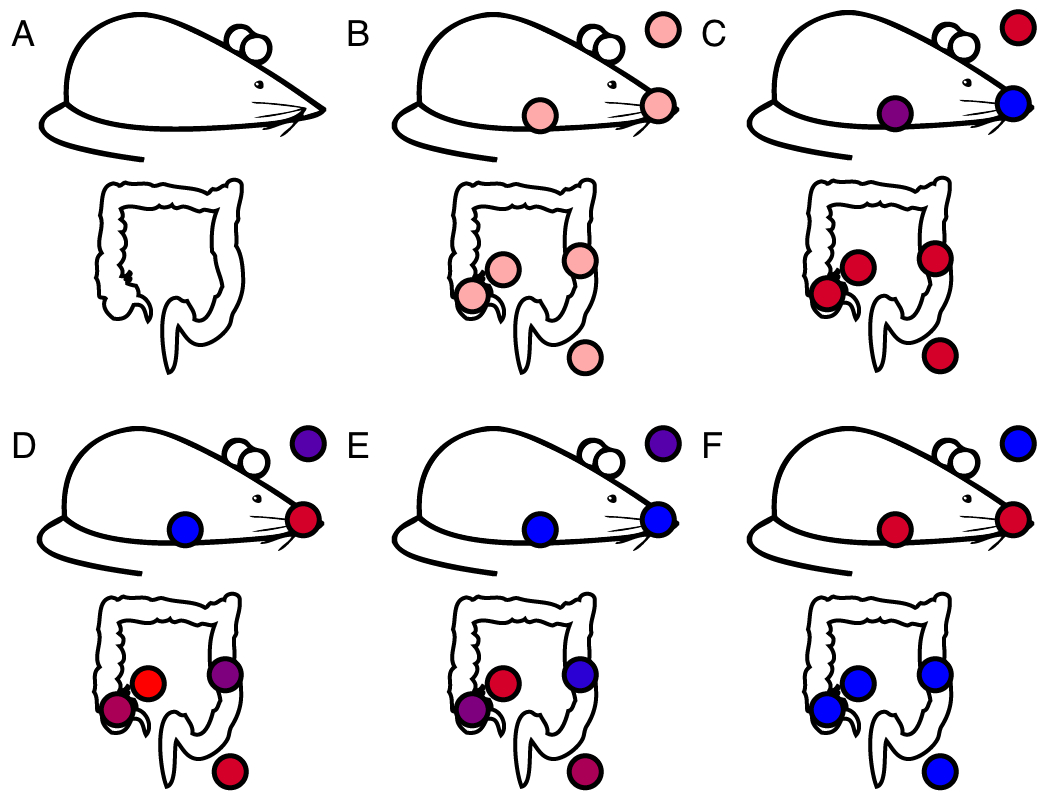
\includegraphics[width=0.75\columnwidth]{chapter_book_figures/Figure_19.jpg}
\caption[Image representing the mouse and its gastrointestinal tract]{\textbf{Image representing the mouse and its gastrointestinal tract.}
A) Raw image without samples. B) Image in SitePainter with samples. C-D)
PCoA axis 1 and 2, in red high values, in blue low values, similar colors represent
similar communities. E-F) Taxonomic distributions of (E) Betaproteobacteria and (F)
Gammaproteobacteria, in red high abundance, in blue low abundance.}
\label{bfigure19}
\end{figure}

Now, we can open this image in SitePainter by clicking on the pencil/flower image on
the right corner, choosing “Open Image”, and select our file. Then we add the places
that we want to color using the rectangle or ellipsoid tool, Figure ~\ref{bfigure19}-B.
Now we need to make our samples in the image match the names of the sample names from our
files; for this we need to click on “\texttt{Elem. -> Click to update}” on the right menu,
this will show us the current sample names in the image; then, we double click on each one
and change the name to make it match the sample name in the mapping file. Note that
SitePainter does not accept sample names with dots (.), so if the sample name has this character,
we need to replace it with an underscore (\_). We do not need to change the \gls{qiime} files, as this
will happen automatically in SitePainter. When we hover over each name, the sample will change color,
facilitating the identification of the image we are selecting. If different sites have the same name,
they will be colored with the same value from the \gls{qiime} output files.

The final step is to load the resulting \gls{qiime} files. To do this, we use the Metadata loader
on the top left of the menu. This opens the file. We then move the right menu to the “Meta.”
tab. Here we can select which column we want to use for coloring, and then click “Color elements”,
to select more, Figure ~\ref{bfigure19}-C-F. For detailed instructions about changing colors and
other details visit SitePainter's website \footnote{\url{http://sitepainter.sourceforge.net/tutorials/index.html}}.

\subsection{Other features}
\subsubsection{Testing linear gradients, including time series analysis}

Recent microbiome surveys have started integrating gradients (commonly over time) in their study design.
We will discuss a first and general approach for those cases, using the Moving Pictures of the Human
Microbiome Dataset \cite{Caporaso2011}, where two subjects were sampled daily for up to 396 days in three
different body sites (sebum, saliva and feces). Note that the mouse dataset that we use as a primary example
lacks a natural temporal ordering in the study design, so we can not use it as an example for this analysis.

PCoA plots provide a snapshot about the relative communities of many samples condensed in a single figure.
However, coloring the points in PCoA space according to a color gradient can be very difficult to understand.
A first approach in this case is to connect the samples belonging to the same subject/treatment subsequently
sorted using the values in the gradient, i.e. one timepoint after the other (see Figure ~\ref{bfigure20} b).
An interactive plot like this can be generated using the following command:

\begin{lstlisting}[language=bash]
make_3d_plots.py \
 -i $PWD/moving_pictures/unweighted_unifrac_pc.txt \
 -m $PWD/moving_pictures/merged_columns_mapping_file.txt \
 -o $PWD/moving_pictures/vectors \
 --add_vectors=BODY_SITEHOST_SUBJECT_ID,DAYS_SINCE_EPOCH
\end{lstlisting}

\begin{figure}[htbp]
\includegraphics[width=\columnwidth]{chapter_book_figures/Figure_20.jpg}
\caption[Beta diversity plots for the moving pictures dataset using unweighted UniFrac as the dissimilarity metric]{\textbf{Beta diversity plots for the moving pictures dataset using unweighted UniFrac as the dissimilarity metric.}
(a) PCoA plot colored by the body site and subject. (b) PCoA plot colored by the body
site and subject with connecting lines between samples. Note in (b) that these lines
allow us to track the individual body sites with a different approach.}
\label{bfigure20}
\end{figure}

An important thing to note here is that because we want to track each of the three
body-sites (SampleTypes) for the two subjects (Subject), we need a column in our
mapping file that allows us to make that distinction. Hence we need to concatenate
those two columns in our metadata mapping file using an external spreadsheet editor or
another tool. Also note that the gradient used is a category named DAYS\_SINCE\_EPOCH
(i.e. the number of days since January 1, 1970). The idea here is to have a common
reference for the collection date of each of the samples.

Although a visualization like the one created in the previous example is often sufficient,
replacing one of the axes in the PCoA plot with the data explaining the gradient provides a
different insight into the analyzed data (See Figure ~\ref{bfigure21}).

\begin{figure}[htbp]
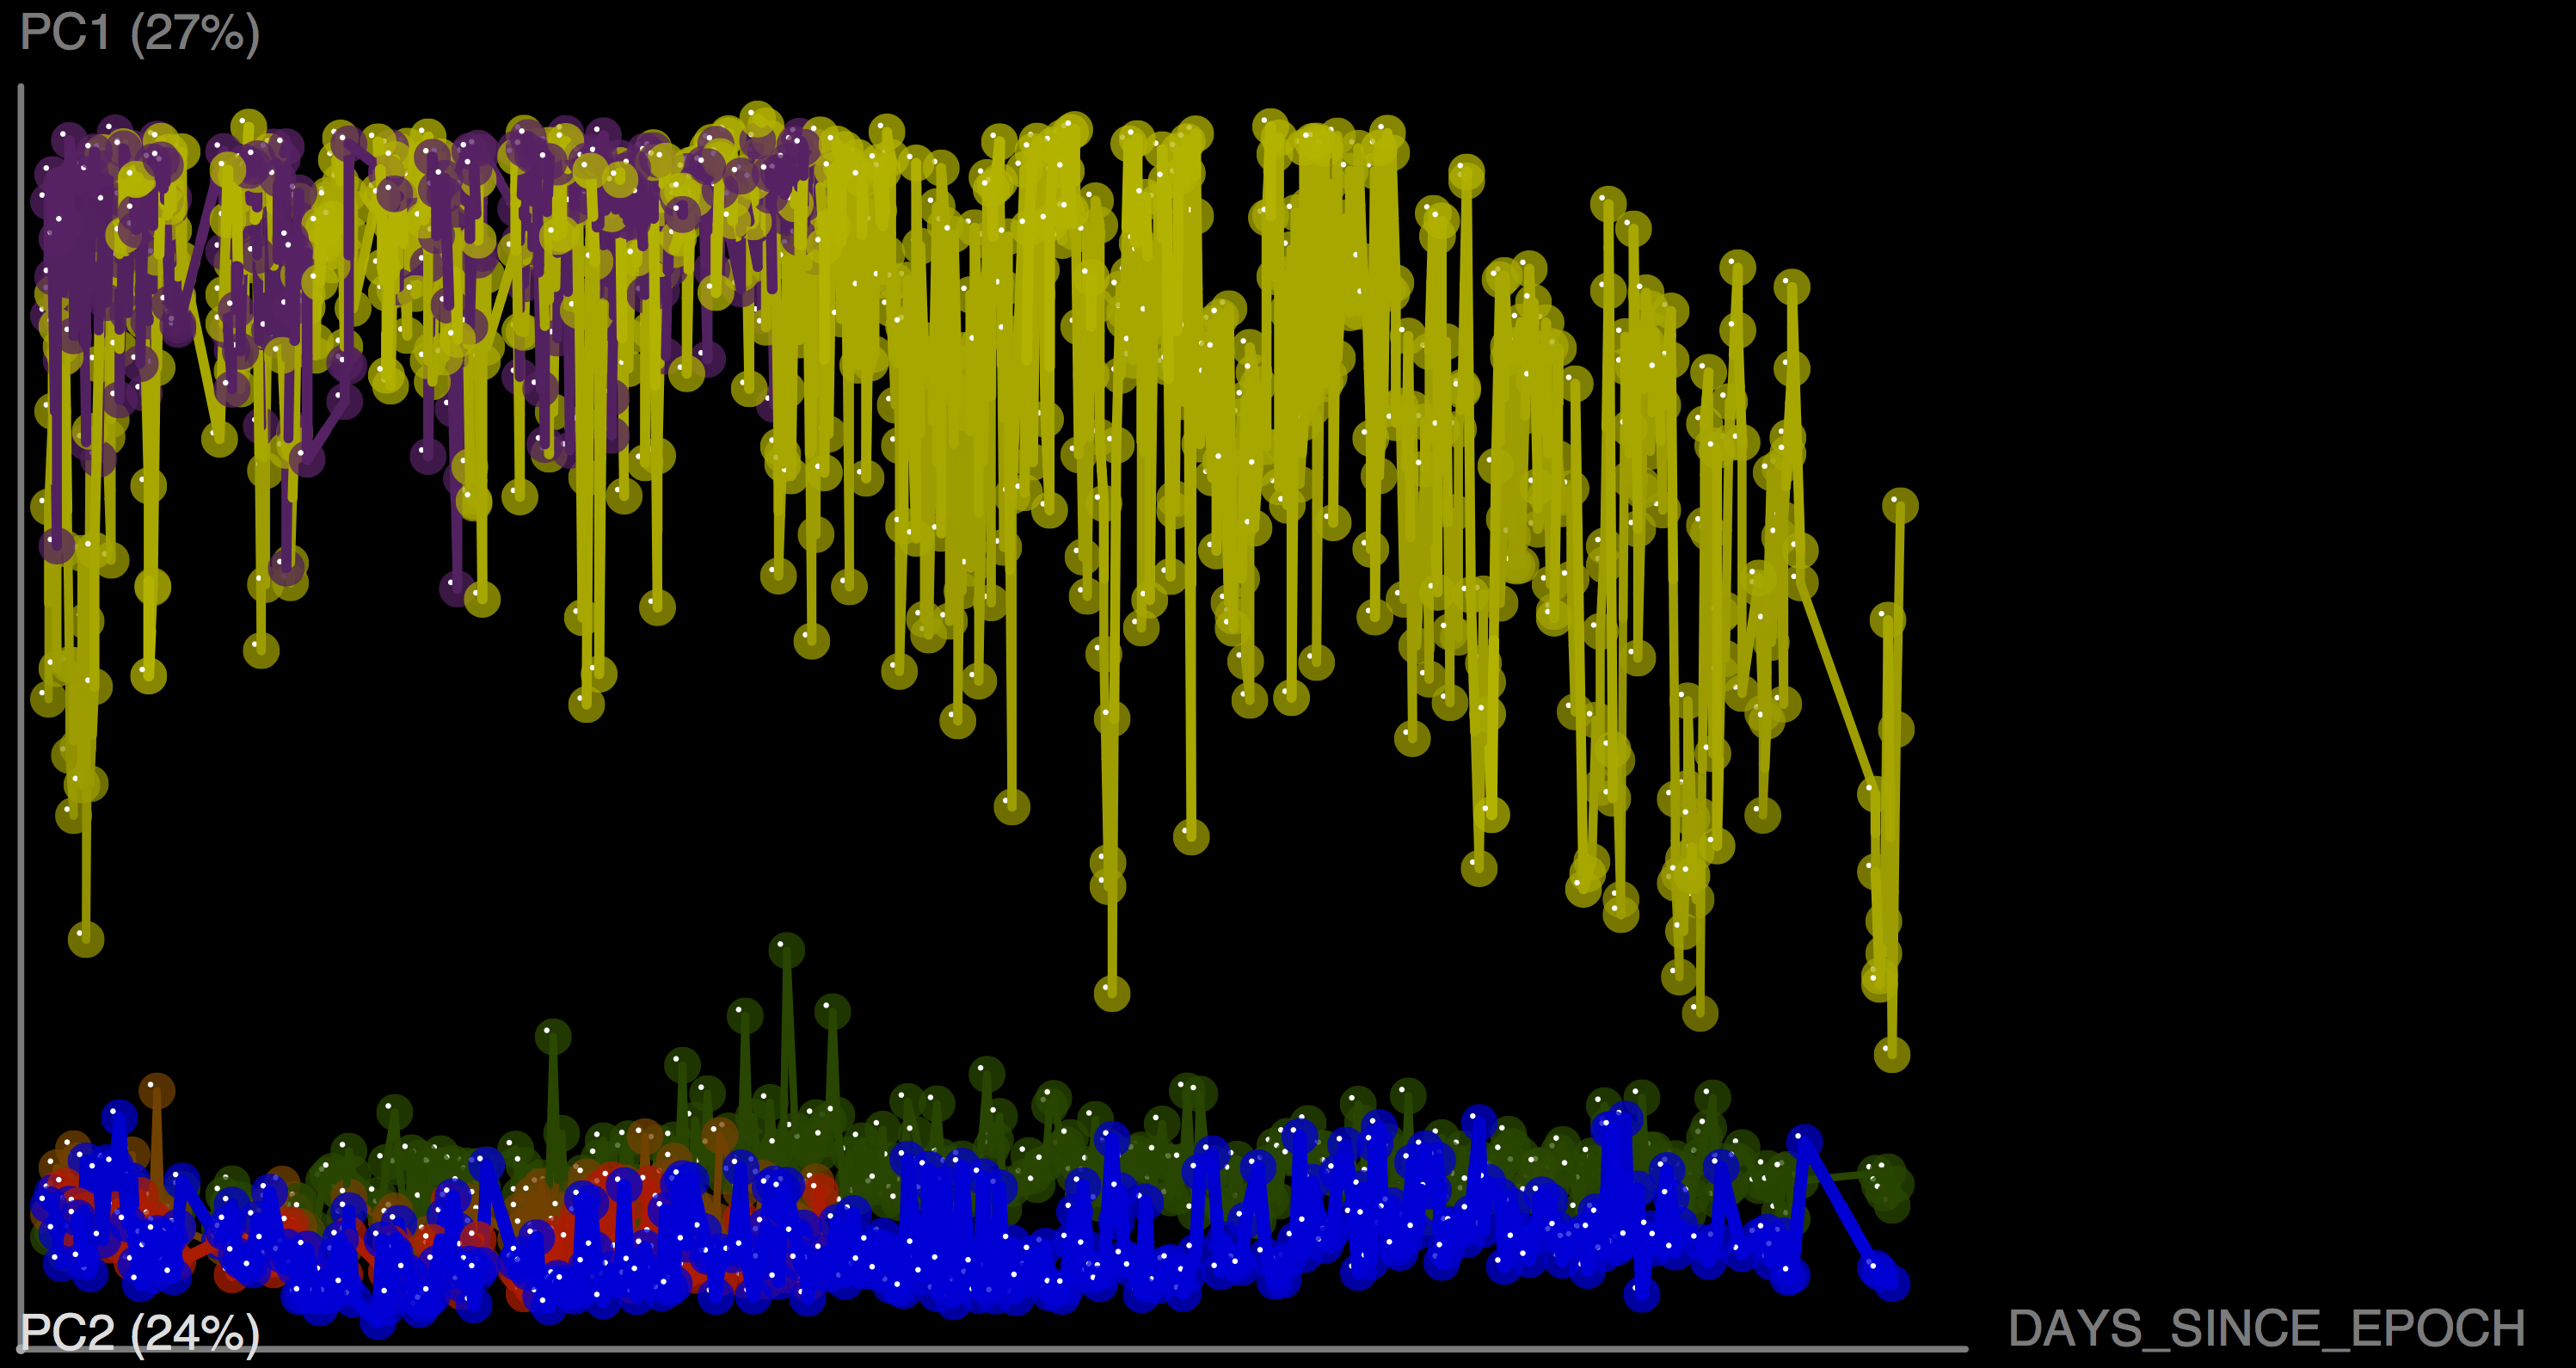
\includegraphics[width=0.75\columnwidth]{chapter_book_figures/Figure_21.jpg}
\caption[Three dimensional plots in which two of the axes are PC1 and PC2 and the other is the day when that sample was collected in reference to the epoch time]{\textbf{Three dimensional plots in which two of the axes are PC1 and PC2 and the other is the day when that sample was collected in reference to the epoch time.}
Although this is not explicitly a beta diversity plot, this representation allows differentiation of the individual trajectories over time.}
\label{bfigure21}
\end{figure}

\begin{lstlisting}[language=bash]
make_3d_plots.py \
 -i $PWD/moving_pictures/unweighted_unifrac_pc.txt \
 -m $PWD/moving_pictures/merged_columns_mapping_file.txt \
 -o $PWD/moving_pictures/vectors \
 --add_vectors=BODY_SITEHOST_SUBJECT_ID,DAYS_SINCE_EPOCH \
 -a DAYS_SINCE_EPOCH
\end{lstlisting}

These visual representations can often identify meaningful patterns. To statistically
support these assertions, one-way analysis of variance (ANOVA) can be used over the
values grouped by a category of interest. In a case where user wants to test for
independence between the variation of one group of trajectories and another,
this command could be used:

\begin{lstlisting}[language=bash]
make_3d_plots.py \
 –i unweighted_unifrac_pc.txt \
 –m mapping_file.txt –o vectors \
 –add_vectors=SampleTypeAndSubject,days_since_epoch \
 –a days_since_epoch --vectors_algorithm avg \
 --vectors_path anova_stats.txt
\end{lstlisting}

\subsubsection{Processing 454 data}

We have described the recommended workflow for conducting microbial community analysis on an
Illumina MiSeq dataset. However, \gls{qiime} can also perform microbial community analysis on the
454 platform. The main advantage of 454 over Illumina is that 454 generates longer sequences,
which can allow a better taxonomy assignment. However, the 454 technology produces fewer reads per
dollar, or per sequencing run \cite{Kuczynski2011}.

The 454 processing workflow differs from the Illumina workflow in the sequence preprocessing.
In this case, the output file from the sequencing facility is a fasta file containing the reads,
and a quality score file which contains the score for each base in each sequence included in the FASTA file.
In this case, the command used for the 454 preprocessing is split\_libraries.py:

\begin{lstlisting}[language=bash]
split_libraries.py \
 -m Fasting_map.txt -f Fasting_Example.fna \
 -q Fasting_Example.qual -o slout
\end{lstlisting}

Similarly to the Illumina processing, this script also performs a quality filtering.
In this case, the quality filtering is based on cut-offs for sequence length, end-trimming
or minimum quality score. However, to successfully remove the read artifacts, a
denoising process has to be performed \cite{Reeder2010} to reduce the impact of homopolymer
runs (runs of the same base). The 454 denoising process is a slow, computationally intensive
problem that does not scale to large datasets, as it is based on flowgram clustering \cite{Quince2011}.

\textbf{Variable length barcodes} Variable-length barcodes are used for two reasons:
to make the number of flows (rather than the number of bases) constant \cite{Frank2009},
or to stagger the reads to reduce bad signal from low complexity at a given position in
the set of amplicons being sequenced. This approach is not recommended today because such
samples are not easily demultiplexed, and there is checksum, like Hamming or Golay, that
allows error-correction and improved sample assignment \cite{Hamady2008}. However,
the \gls{hmp} used variable length barcodes to identify their samples within sequencing runs.
Thus, \gls{qiime} allows demultiplexing such files by using the parameter -b in split\_libraries.py, as follows:

\begin{lstlisting}[language=bash]
split_libraries.py \
 -m map_file_with_variable_length_barcodes.txt \
 -f your_fna.fna -q your_qual.qual \
 -o split_library_output_variable_length/ \
 -b variable_length
\end{lstlisting}

\subsubsection{18S rRNA gene sequencing}
\gls{qiime} can be also used to perform analysis on 18S \gls{rrna} gene sequence data
(in eukaryotes), as well as other markers such as \gls{its}. The main difference
between performing analyses with 18S \gls{rrna} gene data instead of 16S \gls{rrna} gene
data (or \gls{its} data) is the reference database used for \gls{otu} picking,
the taxonomic assignments and the template-based alignment building, since it must
contain eukaryotic sequences.

The recommended database to use as a reference for 18S \gls{rrna} sequences is
the Silva database \cite{Quast2013}. At the time of writing, the most recent
\gls{qiime}-compatible Silva database is the 108 release. Since this database contains
the three domains of life, it can be used as a reference for 18S \gls{rrna} data sets.

When conducting studies mixing 18S \gls{rrna} data and 16S \gls{rrna} data, you
should take into account that picking \gls{otu}s against the Silva database will assign
taxa to all three domains of life. In this case, it is recommended to split the
\gls{otu} table by domain, generating an \gls{otu} for each domain (Archaea, Bacteria and Eukarya).
At this point, each of these tables can be used in downstream analysis in the same
way as performed for 16S \gls{rrna} data.

\subsubsection{Shotgun metagenomics}

Shotgun metagenomics is also supported in \gls{qiime}, although it is still experimental
and it should be used at the user's own risk. Currently, the \gls{qiime} team recommends
the blat method \cite{Kent2002} for searching nucleic acid sequence reads in a
reference database, although usearch \cite{Edgar2010} is also supported. The main
reason for preferring blat against usearch is that protein reference database often
require 64-bit applications, and blat is free of charge, while the 64 bit version of usearch is not.

There are many reference databases (IMG, KEGG, M5nr, among others), and they all
supported by \gls{qiime}, since the user only needs to supply a single fasta file containing
the sequence records. The command that \gls{qiime} provides for mapping reads against the
reference database is map\_reads\_to\_reference.py, and it can be performed in parallel
using the parallel\_map\_reads\_to\_reference.py script.

\subsubsection{Support for QIIME in R}

First published in 1996, “R” is an integrated software application and programming
language designed for interactive data analysis (R Core Team). It is available for Linux,
Mac OS, and Windows free of charge under an open-source license (GPL2). Since its inception,
R has found a niche as a tool for interactive statistical analysis through functional programming.
Primary investigation and inference are performed by writing a series of repeatable commands as
“scripts” that can be recorded and published. This paradigm lends itself well to reproducible
research, and is enhanced substantially by R's integration with tools for literate programming
such as Sweave \cite{FriedrichLeisch2002}, knitr \cite{Xie2013}, and R markdown
\footnote{\url{http://CRAN.R-project.org/package=markdown}}, as well as data graphics. There are thousands
of free and open-source extensions to R (“packages”) available from the main R repository, CRAN,
further organized by volunteer experts into 31 task “views” (which are in fact workflow inventories).
Among these are dedicated package lists relevant to microbiome data, including phylogenetics, clustering,
environmetrics, machine learning, multivariate and spatial statistics, as well as a separate reviewed and
curated repository dedicated to biological statistics called Bioconductor (over 600 packages).

At present, support for \gls{qiime} in R is predominantly achieved through a package called “phyloseq” \cite{McMurdie2013}
dedicated to the reproducible analysis of microbiome census data in R. phyloseq defines an object-oriented data class
for the consistent representation of related (heterogenous) microbiome census data that is independent of the sequencing-
or \gls{otu}-clustering method (storing \gls{otu} abundance, taxonomy classification, phylogenetic relationships, representative
biological sequences and sample covariates). The package supports \gls{qiime} by including functions for importing data
from biom-format files derived from more recent versions of \gls{qiime} (import\_biom) as well as legacy \gls{otu}-taxonomy delimited
files (import\_qiime and related user accessible subfunctions). Later editions of phyloseq ($>$1.5.15) also include an
API for importing data directly from the microbio.me/qiime data repository. In all cases, these API functions
return an instance of the “phyloseq” class that contains the available heterogenous components in “native” R classes.
phyloseq includes a number of tools for connecting with other microbiome analysis functions available in other R packages,
as well as its own functions for flexible graphics production built using ggplot2 \cite{Wickham2009}, demonstrated
in supplemental files and online tutorials. For researchers interested in developing or using methods not directly
supported by phyloseq, nor its data infrastructure, the biom-format specific core functions in phyloseq have been
migrated to an official API in the biom-format project as an installable R package called “biom”, now released on
CRAN. This also includes some biom-format specific functionality that is beyond the scope of phyloseq, though support
for \gls{qiime} is still likely best achieved using phyloseq.

As with some of the earlier examples of \gls{qiime} commands with corresponding output and figures, in this section we
have included some key R commands potentially useful during interactive analysis in the R environment. For simplicity,
show only results related to the open-reference \gls{otu} data, stored in an object in our examples named open,
and imported into R using the phyloseq command import\_biom.

\begin{lstlisting}[language=bash]
open = import_biom(“path-to-file.biom”, …)
\end{lstlisting}

Additional input data files can also be provided to import\_biom, or merged with open after its instantiation.
For clarity, subsets and transformations of the data in open are stored in objects having names that begin
with “open”. As with the remainder of the examples highlighted in this section, the complete code
sufficient for reproducing all results and figures are included in the R Markdown originated document,
Supplemental File 1, which includes several additional examples not shown here, and is available with supporting
files on GitHub\footnote{\url{https://github.com/joey711/navasetal}}.

Although not always very illuminating, a comparison of \gls{otu}-richness between samples or groups of samples can
easily be achieved with the plot\_richness command. For the most precise estimates of richness for most samples,
this should be performed before random subsampling or other transformations of the abundance data. Here open
contains data that has already been randomly subsampled. In figure \ref{bfigure22} we can see that the wild type
samples are generally more diverse (higher richness) and somewhat more variable than the transgenic samples for
essentially all body sites, though the differences between the two mice genotypes are small.

\begin{figure}[htbp]
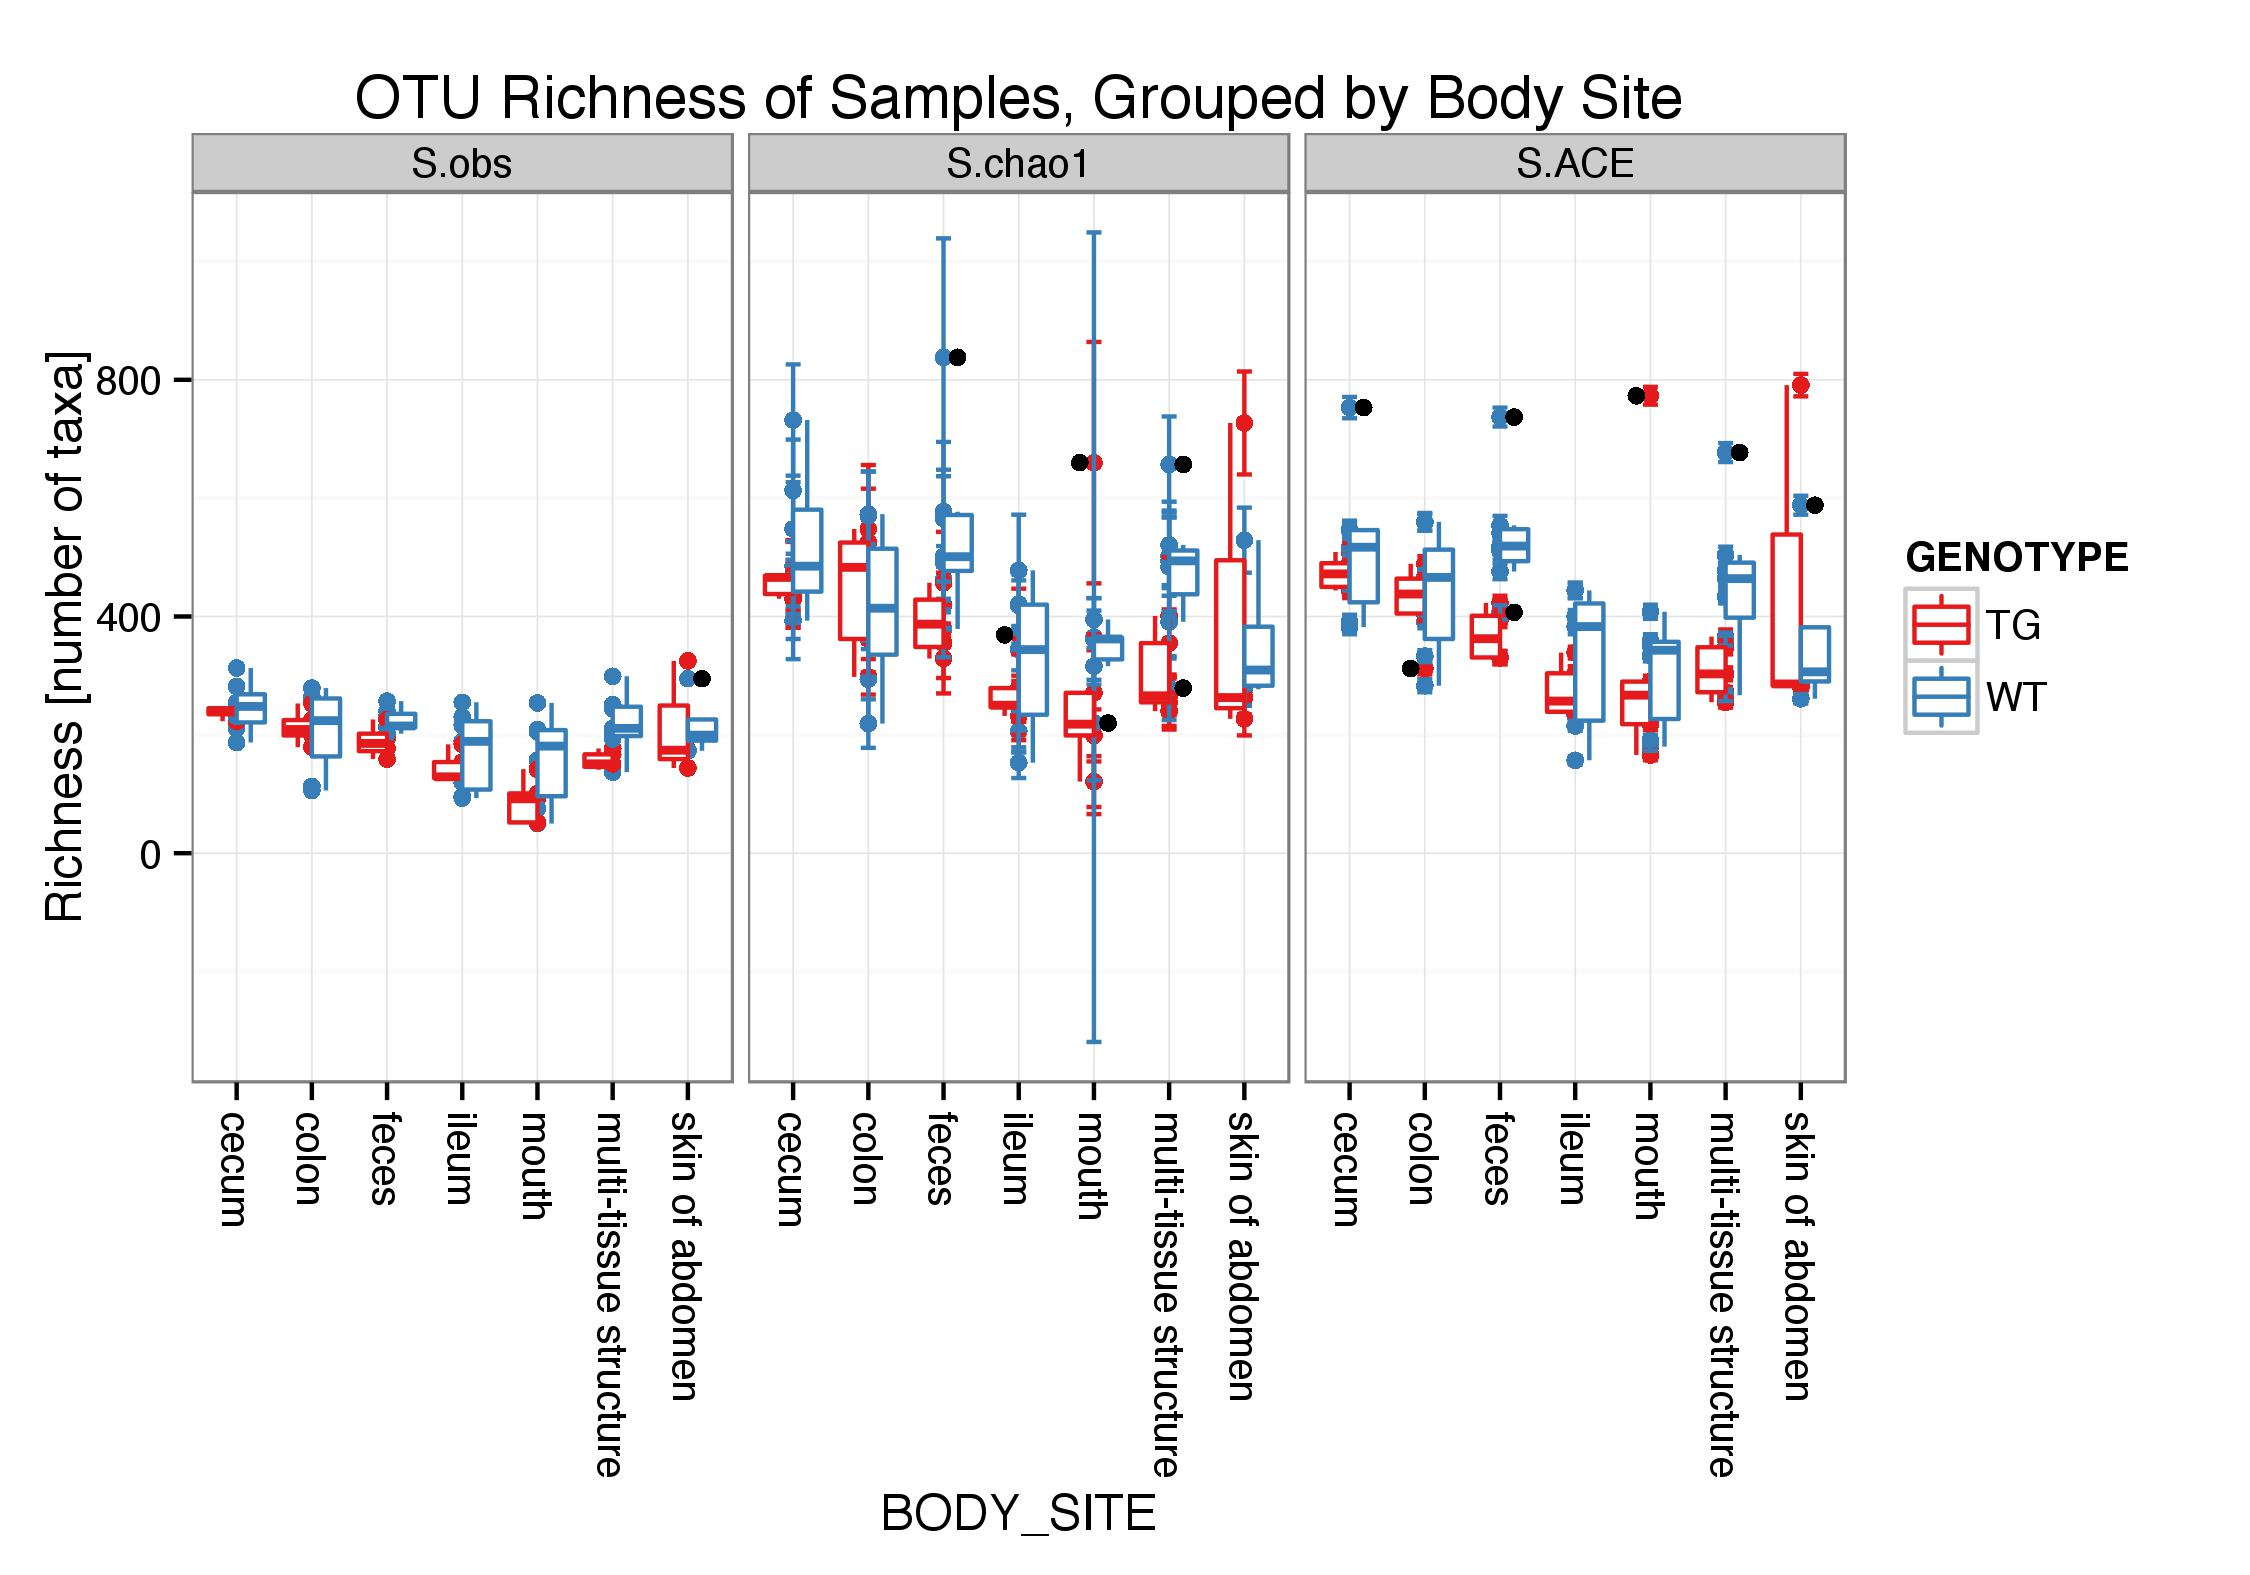
\includegraphics[width=0.75\columnwidth]{chapter_book_figures/Figure_22.jpg}
\caption[Categorically summarized \gls{otu} richness estimates using the plot\_richness function]{\textbf{Categorically summarized \gls{otu} richness estimates using the plot\_richness function.}
Samples are grouped on the horizontal axis according to body site, and color shading
indicates the mouse genotype. The vertical axis indicates the richness estimates in number
of distinct \gls{otu}s, and a separate boxplot is overlaid on the points for each combination
of genotype and body site. The “S.obs”, “S.chao1”, and “S.ACE” panels show the “rarefied”
observed richness, Chao-1 richness, and ACE richness estimates, respectively}
\label{bfigure22}
\end{figure}

\begin{lstlisting}[language=bash]
plot_richness(
  open, x= “BODY_SITE”,
  color = “GENOTYPE”) + geom_boxplot()
\end{lstlisting}

This plot command also illustrates the use of a function in ggplot2, geom\_boxplot,
that instructs the ggplot2 graphics engine to add an additional graphical element –
in this case a boxplot for each of the natural groups in the graphic. These available
additional graphical instructions (called “layers” in the grammar of graphics nomenclature)
are embedded with the returned plot object for subsequent rendering, inspection, or further
modification, allowing for powerfully customized representations of the data.

Here is an example leveraging the abundance bar plot function from phyloseq, plot\_barr,
in order to compare the relative abundances of key phyla between the wild type and
transgenic mice across body sites. The first step was actually some additional data
transformations (not shown, see Supplemental File 1) in order to subset the data to
only major expected phyla (subset\_taxa), merge \gls{otu}s from the same phyla as one entry
(merge\_taxa), and merge samples from the same body site and mouse genotype (merge\_samples).

\begin{lstlisting}[language=bash]
p2 = plot_bar(
  openphyab, “bodysite”,
  fill = “phyla”, title = title)
p2 + facet_gird(∼GENOTYPE)
\end{lstlisting}

From this first bar plot it is clear that all body sites from the average wild type
mouse have Firmicutes as their phylum of largest cumulative proportion, except for the
“feces”, where it is anyway a close call between Firmicutes and Bacteroidetes. By contrast,
some of the average transgenic mice samples have a much higher proportion of Proteobacteria
or Bacteroidetes than the corresponding wild type samples. One drawback to this type of
stacked bar representation is that it is difficult to compare any of the sub-bars except
for those at the bottom. If needed, this can be alleviated by changing the facet\_grid call
such that a separate panel is made for each phyla in the dataset, as follows.

\begin{lstlisting}[language=bash]
p2 + facet_grid(
  phyla ∼ GENOTYPE) + ylim(0, 100)
\end{lstlisting}

With essentially the same effort to produce, the 14 panels of this second bar
plot graphic allow an easy and quantitative comparison of the relative abundances
of each phylum across body sites and genotype.

Microbiome datasets can be highly multivariate in nature, and dimensional reduction
(ordination) methods can be a useful form of exploratory analysis to better understand
some of the largest patterns in the data. Many ordination methods are wrapped in phyloseq
by the ordinate function, and many more are offered in available R packages. Here we
show an example performing multidimensional scaling (MDS) on the precomputed unweighted
UniFrac distance matrix for the open-reference dataset. The ordination result (openUUFMDS)
is first passed to plot\_scree in order to explore the “scree plot” representing the
relative proportions of variability represented by each successive axis. Both
the ordination result and the original data are then passed to plot\_ordination
with sufficient parameters to shade the sample points by genotype, and create
separate panels for each body site.

\begin{lstlisting}[language=bash]
openUUFMDS = ordinate(
 open, “MDS,
 distance = UniFrac[[“unweighted”]][[“open””]])
plot_scree(openUUFMDS, “Unweighted Unifrac MDS”)
plot_ordination(open, openUUFMDS, color = “GENOTYPE”)
+ geom_point(size = 5) + facet_wrap(∼BODY_SITE)
\end{lstlisting}

It appears that a subset of the wild-type samples from all but the mouth and
abdomen-skin body sites cluster toward the left of the plot. This appears to be
the major pattern along the axis that also comprises the greatest proportion of
variability in the dataset. At this stage of analysis it seems worthwhile to try
to identify which \gls{otu} abundances are most different between these groups, and then
perform some formal validation/testing of these differences.

\subsection{Recommendations}
Here, we highlight some of the main aspects to take into account when performing microbial community analysis:

\begin{itemize}
    \item Use the open-reference \gls{otu} picking approach if your data allows it. It
    will reduce the running time and will recover all the diversity in your samples.
    \item Perform an \gls{otu} quality filtering based on abundance, by removing singletons,
    for instance. See \cite{Bokulich2013} for further discussion on how to tune this
    quality filtering and its effects on downstream analysis. Quality filtering is
    critical for obtaining reasonable numbers of \gls{otu}s from a sample.
    \item Consider whether you need to remove specific taxa from your study, such
    chloroplast or host DNA sequences when analyzing microbial datasets.
    \item Remove samples from your study that have low coverage (i.e. low \gls{otu} counts).
    They are likely uninformative and usually indicate low-quality reads.
    \item Rarefy your \gls{otu} table in order to mitigate the differences on the sequencing
    effort, so the downstream diversity analyses won’t be biased by the artificial
    diversity generated due to the difference in sequencing depth.
\end{itemize}

\subsection{Conclusions}
\gls{qiime} is a powerful tool for the analysis of bacterial community allowing researchers
to recapitulate the necessary steps in the processing of sequences from the raw data
to the visualizations and interpretation of the results. Two advantages make \gls{qiime} very
useful: fidelity to the algorithms used, and consistency in the analysis. Fidelity is obtained
because \gls{qiime} wraps existing software, preserving the integrity of the original programs and
algorithms designed, created, and tested by the original authors. Consistency is obtained
because \gls{qiime} can be applied to sequences from different platforms, and once the upstream
process is done; the analysis (downstream) process is the same independent of the sequencing
platform used. These characteristics, together with the fact that \gls{qiime} is open-source software
with continuous support to users via \gls{qiime} forum, have promoted the rapid increase in the \gls{qiime}
user community since its publication \cite{Caporaso2010}.

Downstream and upstream processes are implemented in \gls{qiime} in a way that offers several options
to perform the analyses. In this review, we discuss and demonstrate the principles for each step,
what the scripts do and how to choose between options. Independent of the use of \gls{qiime}, this
review also provides an overview of many of the typical steps in a microbial community analysis
based on analysis of 16S rRNA sequences produced by high-throughput sequencing. Some of these tools
are well developed with a long history in general ecology, whereas others are still in rapid development;
we encourage microbial ecologists and bioinformaticians to work together to create, develop and implement
new strategies and tools that allow further exploration of this fascinating field.

\subsection{Acknowledgments}
We thank William A Walters and Jessica Metcalf for productive discussion and their
useful comments about \gls{qiime}. We also acknowledge Manuel Lladser for helping
collect the dataset and allowing us to use it, and the IQBio IGERT grant for funding
data collection. JANM is supported by a graduate scholarship funded jointly by the Balsells
Foundation and by the University of Colorado at Boulder. SH is partially supported by
NIH grant R01 GM086884. This work was partially supported by the Howard Hughes Medical Institute.

\section{Advancing our understanding of the human microbiome using QIIME}\label{section_book}
Add paper: ``Advancing our understanding of the human microbiome using QIIME''. J. A. Navas-Molina, et al. \emph{Methods in Enzymology}, 2013, DOI: 10.1016/B978-0-12-407863-5.00019-8.

\section{Bottlenecks in large scale microbial studies: sequence clustering}\label{section_bottlenecks}

Section~\ref{section_book} described a microbial community analysis pipeline in depth.
In that pipeline, one of the most time-consuming steps is performing
sequence clustering (also known as \gls{otu} picking). Sequence
clustering is the processing step that groups sequences into \gls{otu}s
based on sequence similarity. The \gls{otu}s found in a sample are used as an
approximation of the species richness in the given niche. Sequence similarity is
computed using pairwise sequence alignment \cite{Needleman1970, Smith1981}, an expensive
computational task that is quadratic in the length of the input sequences and
the number of input sequences. With
datasets containing from a few hundred thousand reads to a few billion
reads \cite{Goodwin2016}, performing all pairwise sequence alginments is too
computationally expensive to be performed in a timely manner. The sequence clustering
problem shares characteristics with the biological sequence database search problem,
which has been studied for more than 30 years. Sections~\ref{subsection_openref},
~\ref{subsection_soa} and~\ref{subsection_deblur}, contain a summary of my
contributions to optimize the sequence clustering step of microbial community
datasets analysis.

Section~\ref{subsection_openref} has been adapted from the original publication in
``Subsampled open-reference clustering creates consistent, comprehensive OTU
definitions and scales to billions of sequences''. J. R. Rideout, Y. He,
J. A. Navas-Molina, W.A. Walters, L. K. Ursell, S. M. Gibbons, J. Chase,
D. McDonald, A. Gonzalez, A. Robbins-Pianka, J. C. Clemente, J. A. Gilbert,
S. M. Huse, H. W. Zhou and R. Knight \emph{PeerJ}, 2014, DOI: 10.7717/peerj.545.

Section~\ref{subsection_soa} has been adapted from the original publication in
``Open-source sequence clustering methods improve the State of the Art''.
E. Kopylova, J. A. Navas-Molina, C. Mercier, Z. Z. Xu, F. Mahe, Y. He, H. Zhou,
T. Rognes, J. G. Caporaso, R. Knight \emph{mSystems}, 2016, DOI: 10.1128/mSystems.00003-15

Section~\ref{subsection_deblur} has been adapted from the original publication in
``Deblur rapidly resolves single-nucleotide community sequence patterns''.
A. Amir, D. McDonald, J. A. Navas-Molina, E. Kopylova, J. T. Morton, Z. Z. Xu,
E. P. Kightley, L. R. Thompson, E. R. Hyde, A. Gonzalez, R. Knight \emph{mSystems},
2017, DOI: 10.1128/mSystems.00191-16

\subsection{Subsampled open-reference clustering creates consistent, comprehensive OTU definitions and scales to billions of sequences}\label{subsection_openref}

Section~\ref{section_book} \hspace{0.01cm} described \hspace{0.01cm} three \hspace{0.01cm} different \gls{otu} picking approaches:
closed-reference, \emph{de-novo} and open-reference. The open-reference approach
was the recommended approach because it offers benefits over the other two
approaches. The open-reference approach run time is shorter than
the \emph{de-novo} approach because it includes a parallel closed-reference step.
Additionally, the open-reference approach doesn't discard any sequences from
the input dataset because it contains a \emph{de-novo} step. However, if the microbial
organisms present in an environment have not been previously characterized and included
in the reference database, many sequences will fail to cluster
during the closed-reference step, generating long running times on the \emph{de-novo} step.
To further reduce the running time of the open-reference approach, we presented
a new approach: the subsampled open-reference approach \cite{Rideout2014}.

The following text has been adapted from the original publication in
\textsl{PeerJ, 2014}. As a contributor to this manuscript, I was involved in the
design of the subsampled open-reference pipeline, contributed
to the source code, performed some of its evaluations, wrote sections of the
manuscript and reviewed drafts of the manuscript.

A detailed description of the workflow is illustrated in Figure~\ref{sub_open_ref_fig1}.
It is implemented using UCLUST v1.2.22q \cite{Edgar2010} for clustering in \gls{qiime}-1.6.0 \cite{Caporaso2010}
and later, though any sequence clustering software that provides support for \emph{de-novo}
and closed-reference clustering could be substituted for UCLUST. The inputs
provided to this method are demultiplexed,
quality-filtered sequences, and a reference sequence collection (for example,
the Greengenes 13 8 97\% \gls{otu} representative sequences \cite{DeSantis2006, McDonald2012}).
First, sequences are clustered in parallel using a closed-reference \gls{otu} picking
workflow, where sequences are queried against the reference database at percent
identity \emph{s} (default 97\%). If a read matches a reference sequence at greater
than or equal to \emph{s}\% identity, it is assigned to the \gls{otu} defined by that
reference sequence. These are referred to as the reference \gls{otu}s. Next, a
random subsample of \emph{n}\% (\emph{n} should be small, the default value in
\gls{qiime} 1.8.0-dev and earlier is 0.1\%) of the sequences that failed to match
the reference sequence collection are clustered \emph{de-novo}, and the cluster
centroids for all resulting \gls{otu}s are used to define a new reference sequence
collection. Those \gls{otu}s are referred to as the new reference \gls{otu}s.
The sequences that were not included in the random subsample that was clustered
\emph{de-novo} then go through an additional round of parallel closed-reference \gls{otu}
picking, this time where they are clustered against the new reference \gls{otu}s based
on matching a sequence in the new reference sequence collection at greater than
or equal to \emph{s}\% identity. This creation of a “new reference database”
allows us to harness the parallelization of our closed-reference \gls{otu} picking
pipeline, greatly decreasing the time it takes for sequences that fail to hit the
initial reference database to be clustered into \gls{otu}s. In the final clustering
step, sequences that fail to hit a reference sequence during this final
closed-reference \gls{otu} picking step are clustered \emph{de-novo}. These are
referred to as the clean-up \gls{otu}s. Finally, the reference \gls{otu}s, new
reference \gls{otu}s, and clean-up \gls{otu}s are combined into a single \gls{otu}
table (i.e., table of counts of \gls{otu}s on a per-sample basis, as described in
\cite{McDonald2012BIOM}), and this table, as well as a filtered table excluding
\gls{otu}s with counts less than or equal to a user-defined threshold \emph{c},
are provided to the user. By default, \emph{c = 2}, so each \gls{otu} is
observed at least twice (i.e., singleton \gls{otu}s are excluded). Because
many more of the sequences can be clustered using closed-reference \gls{otu}
picking in this workflow, it can run in far less time than classic
open-reference \gls{otu} picking.

\begin{figure}[htbp]
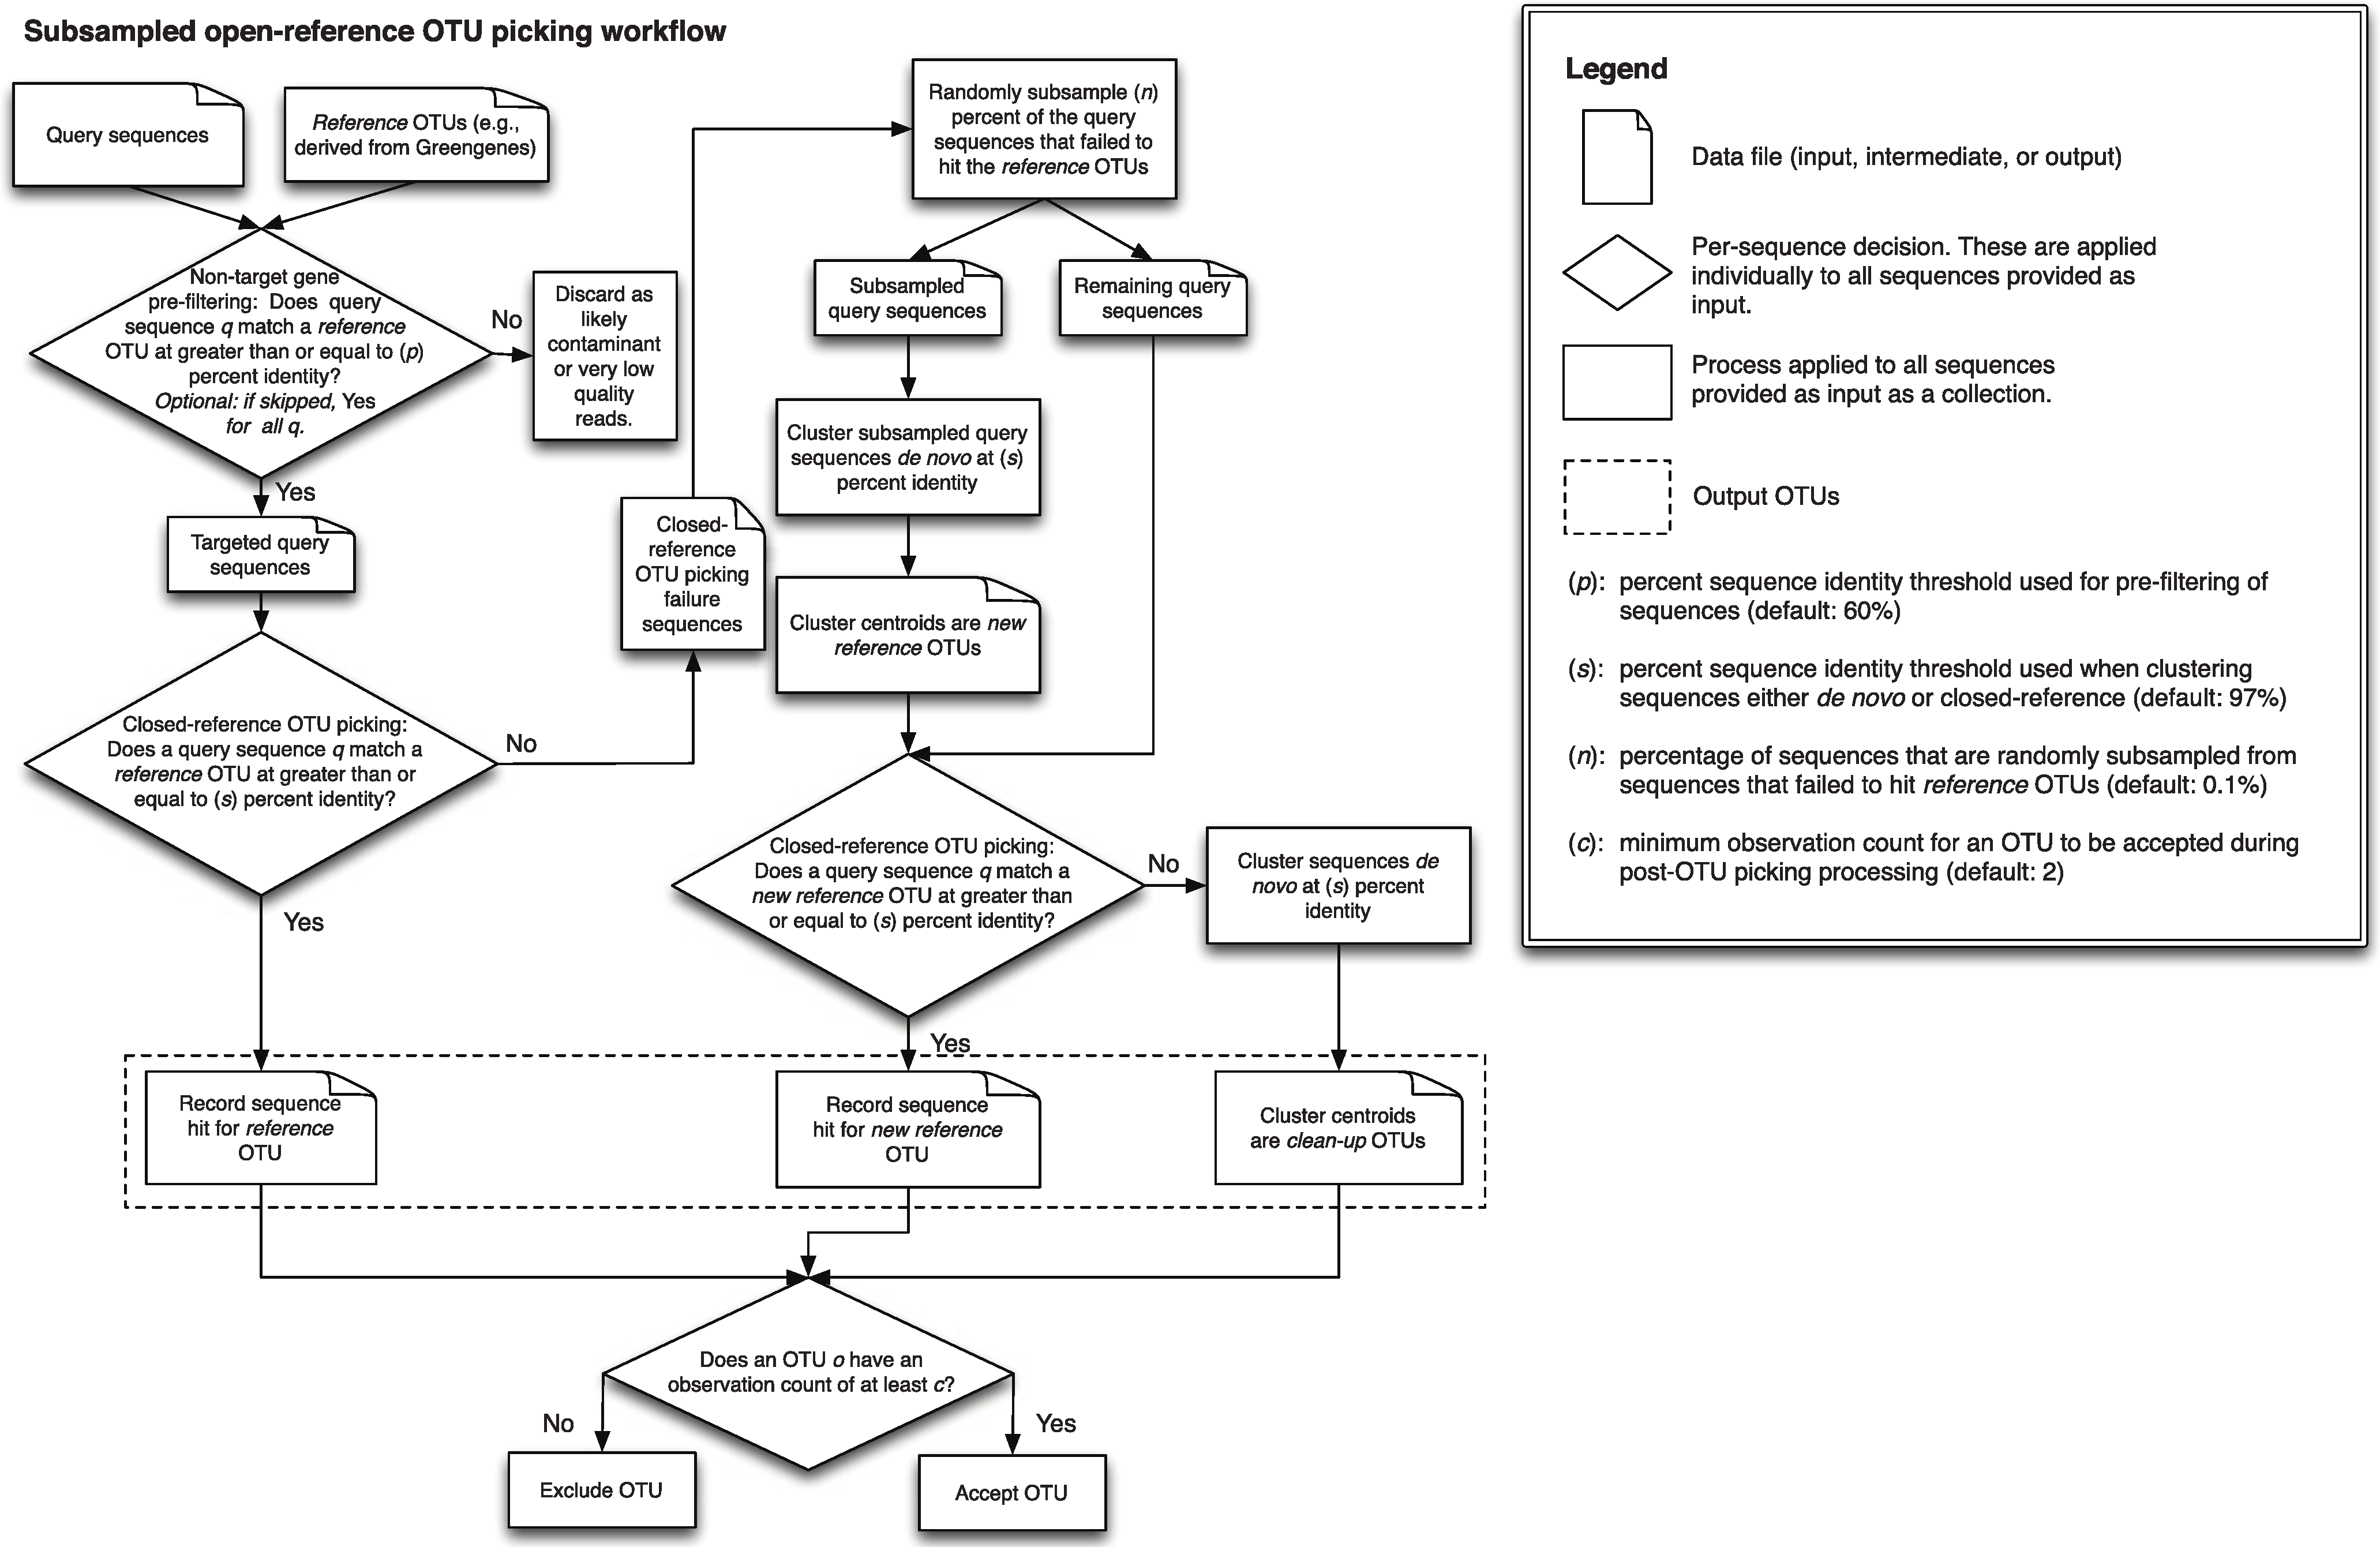
\includegraphics[width=\columnwidth]{chapter_otupicking_figures/workflow.png}
\caption[Schematic of the subsampled open-reference OTU picking algorithm]{\textbf{Schematic of the subsampled open-reference OTU picking algorithm.}}
\label{sub_open_ref_fig1}
\end{figure}

We validated the subsampled open-reference \gls{otu} picking workflow by comparing it
to the classic (i.e. non subsampled) open-reference clustering methods on three
different datasets: the Lauber ``88 Soils'' study \cite{Lauber2009} (referred to
as \emph{88-soils} here), the Caporaso ``Moving Pictures'' study \cite{Caporaso2011}
(referred to as \emph{moving-pictures} here), and the Costello ``Whole Body'' study
\cite{Costello2009} (referred to as \emph{whole-body} here) using three metrics.
First, we tested the correlation between sample alpha diversities (\gls{otu} counts,
i.e. \gls{qiime}'s \emph{observed species} metric and \gls{pd} \cite{Faith1992}) based
on subsampled open-reference \gls{otu} picking and the classic open-reference clustering.
Next, we tested whether beta diversity patterns (as determined by weighted and
unweighted UniFrac \cite{Lozupone2005} distances between samples) were consistent across \gls{otu}
picking protocols, based on Mantel tests \cite{Mantel1967} with 1,000 Monte Carlo iterations.
Finally, we tested whether the same taxonomic profiles were obtained on a per-sample
basis using each of the \gls{otu} picking methods. It is important to note that
we are not trying to assess whether one method is better than another using these metrics.
Instead we are testing whether the methods give highly correlated results.

Alpha diversity (whole-body \gls{pd} Pearson \emph{r = 0.989}; 88-soils \gls{pd}
Pearson \emph{r = 0.930}; moving-pictures \gls{pd} Pearson \emph{r = 0.996}),
beta diversity (whole-body unweighted UniFrac Mantel \emph{r = 0.948};
88-soils unweighted UniFrac Mantel \emph{r = 0.939}; moving-pictures
unweighted UniFrac Mantel \emph{r = 0.991}) and taxonomic summaries (whole-body:
\emph{r = 0.999} at phylum level, 0.999 at species level; 88-soils \emph{r = 0.999}
at phylum level, \emph{r = 0.999} at species level; moving-pictures \emph{r = 0.999}
at phylum level, \emph{r = 0.999} at species level) were highly correlated between
classic and subsampled open-reference \gls{otu} picking. Minor differences likely
arise from the non-deterministic step of rarefying all samples to even sampling
depth before comparing samples. These results suggest that subsampled open-reference
picking yields the same results as classic open-reference \gls{otu} picking,
including identical numbers of sequences failing to hit the reference database,
and therefore is a suitable replacement.

\subsection{Open-source sequence clustering methods improve the State of the Art}\label{subsection_soa}

Section~\ref{subsection_openref} described a faster approach to perform open-reference
\gls{otu} picking. The \gls{otu}s quality and the final running time are dependant
on the actual underlying tool being used to perform the \gls{otu} picking. In the
previous section, UCLUST v1.2.22q \cite{Edgar2010} was used, which was
developed in 2010, and had become the default option for researchers performing
micorbial community analysis. Since then, new tools have been published in the
literature and a comprehensive benchmark of those tools was needed to evaluate if
a new, faster, more accurate tool was available.

The following material has been adapted from the original publication in
\textsl{mSystems, 2016}. As a contributor to this manuscript, I was involved in
the integration of the new tools in \gls{qiime}, contributed to the experimental
design, provided input about the compatible \gls{otu} definitions,
performed some of the benchmarks, wrote sections of the manuscript and
reviewed drafts of the manuscript.

Between 2012 and 2015, four new sequence-clustering tools have emerged: OTUCLUST
from the Micca package \cite{Albanese2015}, Swarm \cite{Mahe2014, Mahe2015},
SUMACLUST (C. Mercier, F. Boyer, E. Kopylova, P. Taberlet, A. Bonin, and E. Coissac,
submitted for publication), and SortMeRNA \cite{Kopylova2012}. These tools
include open-source implementation, and the latter three implement multilevel
parallelization, providing excellent potential alternatives to UCLUST \cite{Edgar2010}.
In this study, we evaluated these new open-source tools and compared them against
UCLUST and USEARCH, two commonly used options available in \gls{qiime}, UPARSE
\cite{Edgar2013}, the latest USEARCH amplicon analysis pipeline, and the three
hierarchical clustering algorithms available in mothur \cite{Schloss2009}.

A variety of datasets were chosen to evaluate the performance of these open-source
\gls{otu} clustering approaches relative to \gls{qiime}’s UCLUST/USEARCH-based
\gls{otu} clustering approaches as well as UPARSE. Two 16S \gls{rrna} gene simulated
datasets were generated as FASTQ files. The first one (\emph{sim\_even}) represents
an even distribution of 1,076 species, randomly subsampled from the Greengenes
97\% \cite{DeSantis2006, McDonald2012} database and computationally amplified at
the same depth (100 reads/amplicon) and length (150 \gls{bp}) using
PrimerProspector \cite{Walters2011} for extracting the V4 region and the ART \cite{Huang2012}
simulator for amplification and sequencing simulation. The second data set (\emph{sim\_staggered})
represents the same 1,076 species as the \emph{sim\_even} data set but amplified at
different (random) species abundance levels. We used four different previously published
mock community data sets: three 16S \gls{rrna} gene mock community data sets
(\emph{Bokulich\_2}, \emph{Bokulich\_3}, and \emph{Bokulich\_6}) from Bokulich
et al. \cite{Bokulich2013} and an 18S gene (\emph{mock\_nematodes}) data set from
Porazinska et al. \cite{Porazinska2009}. Finally, we also used three previously
published natural data sets: a 16S \gls{rrna} gene soil data set (\emph{canadian\_soil})
from Neufeld et al. \cite{Neufeld2011}, a 16S \gls{rrna} gene human data set (\emph{body\_sites})
from Costello et al. \cite{Costello2009}, and an 18S \gls{rrna} gene soil data set
(\emph{global\_soil}) from Ramirez et al. \cite{Ramirez2014}.

Performance was evaluated using a variety of metrics, including the accuracy of
\gls{otu} and taxonomic assignments, alpha diversity (within-sample diversity),
beta diversity (between-sample diversity), and taxonomic correlation. All tools
showed increased precision after the removal of singleton \gls{otu}s (\gls{otu}s
consisting of only one sequence), so all results presented here have had singleton
\gls{otu}s removed. Table~\ref{stateArtT2} summarizes basic performance results
for all software.

\begin{sidewaystable}[htbp]
\caption[Benchmark summary]{\textbf{Benchmark summary.} \gls{otu} counts do not
include singletons. F measure (F1) is for assigned taxonomies at the genus level.
The \gls{pd} whole-tree column for \emph{Bokulich\_2} and \emph{Bokulick\_3}
represent \gls{pd} intervals across various sampling depths. Procrustes $M^2$
(the sum of squared deviations or the dissimilarity of two datasets for UniFrac
\gls{pcoa}) and rho (Pearson's correlation coefficient for taxonomies at genus
level) values are with repect to UCLUST (default for \gls{qiime} versions 1.0.0
to 1.9.1). Monte Carlo $P$ values were not included, since all values were
$<0.05$ except for \emph{de novo} usearch52 versus uclust ($P = 0.09$). The darkest
blue shades represent the highest F1 scores, while the darkest red shades represent
results closest to those obtained with UCLUST}
\label{stateArtT2}
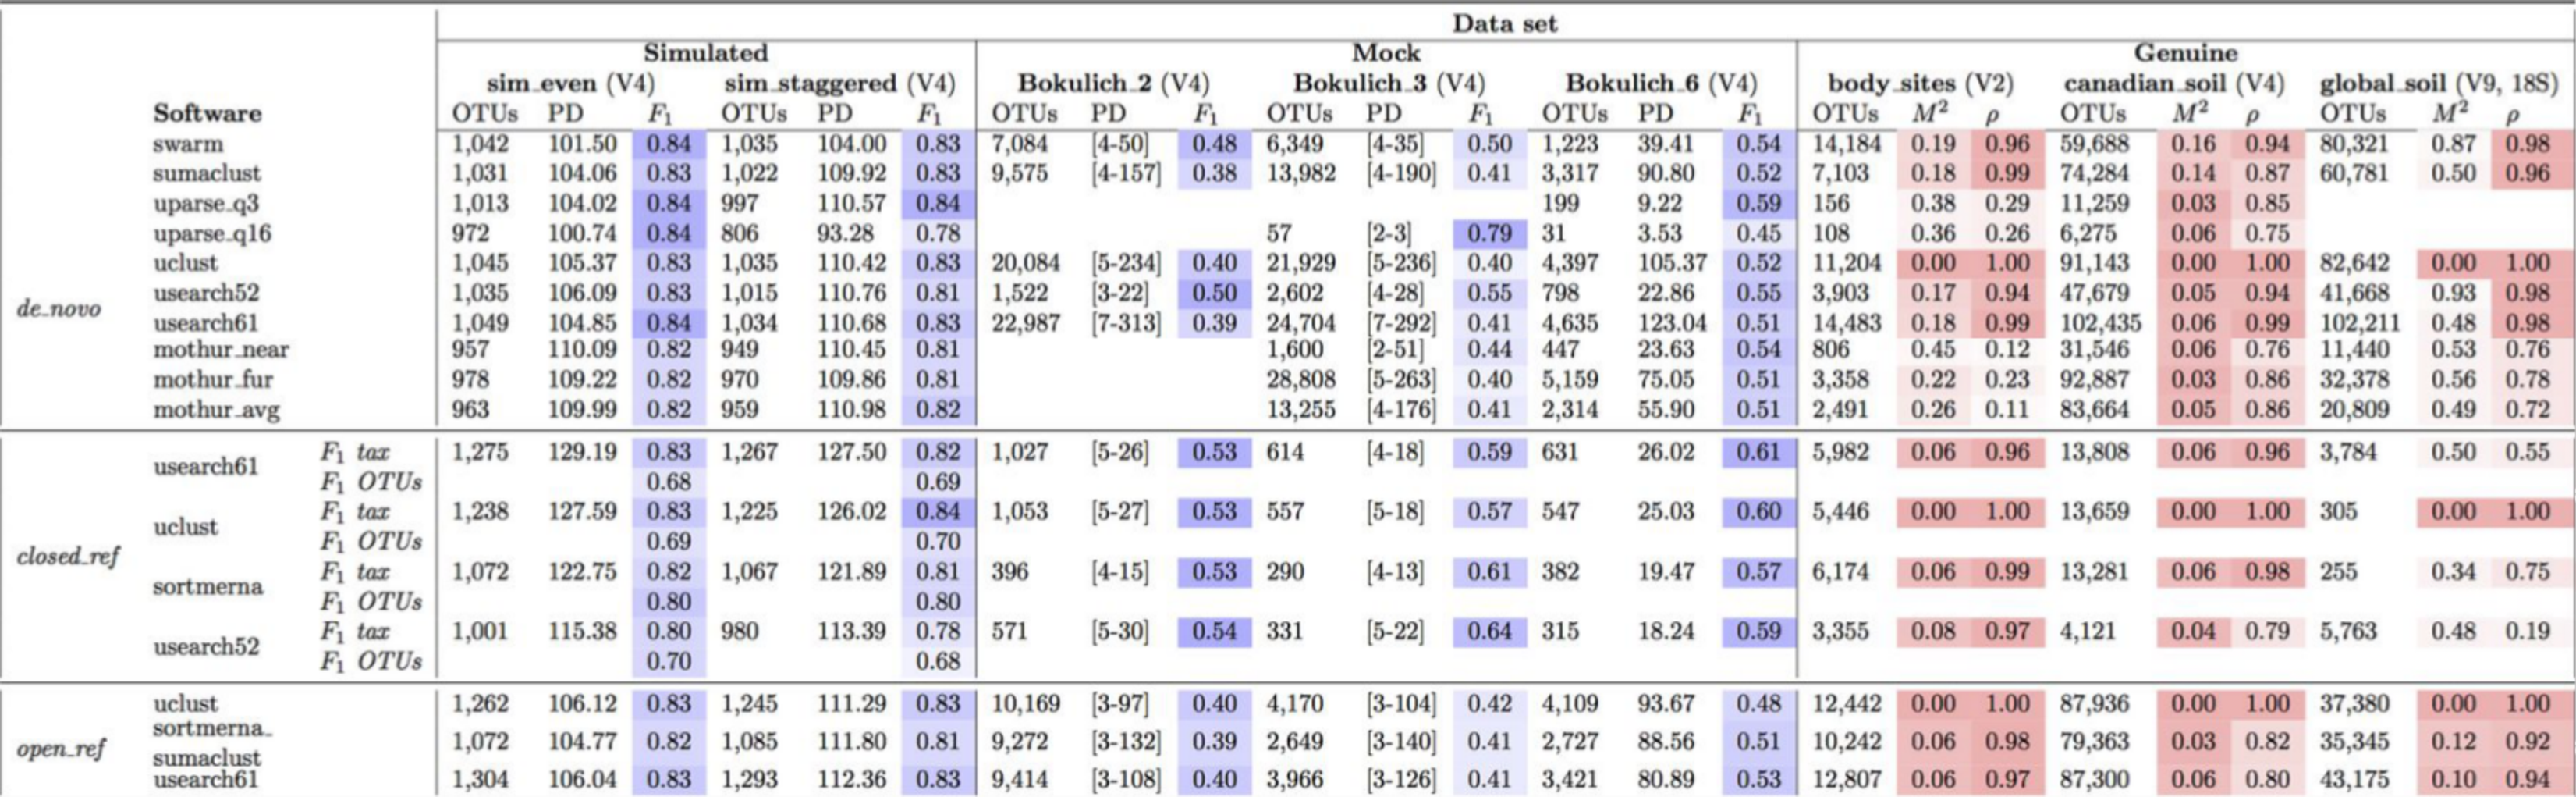
\includegraphics[width=\columnwidth]{chapter_otupicking_figures/stateArtT2.pdf}
\end{sidewaystable}

We found that Swarm, SUMACLUST, UCLUST, and UPARSE (with relaxed parameters)
performed equally well on simulated datasets where the ground truth was well
established, with \emph{mothur\_average} and OTUCLUST closely behind. Despite
this controlled chimera-free environment, UPARSE with recommended parameters
reported the lowest accuracy for the \emph{sim\_staggered} data set, implying
that stringent quality filtering can cause a significant underestimation of
species abundance and diversity and lead to incorrect biological results. For
the mock communities, most tools were able to correctly detect the expected
number and identity of genera, but only UPARSE reported significantly fewer
false-positive taxa (followed by OTUCLUST and USEARCH). For UPARSE, this was
expected, as a large proportion of reads was filtered out prior to clustering,
leaving evidence of only the most abundant taxa (\gls{otu}s comprised of
hundreds of thousands of reads). The majority of false-positive taxa reported
by other tools were low-abundance \gls{otu}s that could be mapped to \gls{blast}’s NT
database with very high similarity ($E$ value, $<1e−50$). If the user’s primary
goal is to focus on the most abundant microbial profiles, low-abundance \gls{otu}s
may be filtered out postclustering, but care should be taken, because such low-abundance
\gls{otu}s can be important members of communities \cite{Shade2014}.

Although most open-source tools report an increased run time in comparison to UCLUST
and USEARCH ~\ref{stateArtF5}, they provide the benefit of finding significantly
fewer \gls{otu}s. In the case of SortMeRNA, longer reads (~150 \gls{bp}) are quicker
to align than the same number of shorter reads (~100 \gls{bp}) due to many fewer
high-scoring candidate reference sequences to analyze. Moreover, all of these tools
support multilevel multithreading and can easily scale to modern big-data processing
demands. An alternative to reducing run time is to filter out a substantial
number of reads, as done by UPARSE; unfortunately, the filtering parameters are
sensitive to different data, and choosing them manually by trial and error can be
a time-consuming task with unpredictable outcomes in diversity.

\begin{figure}[htbp]
\begin{center}
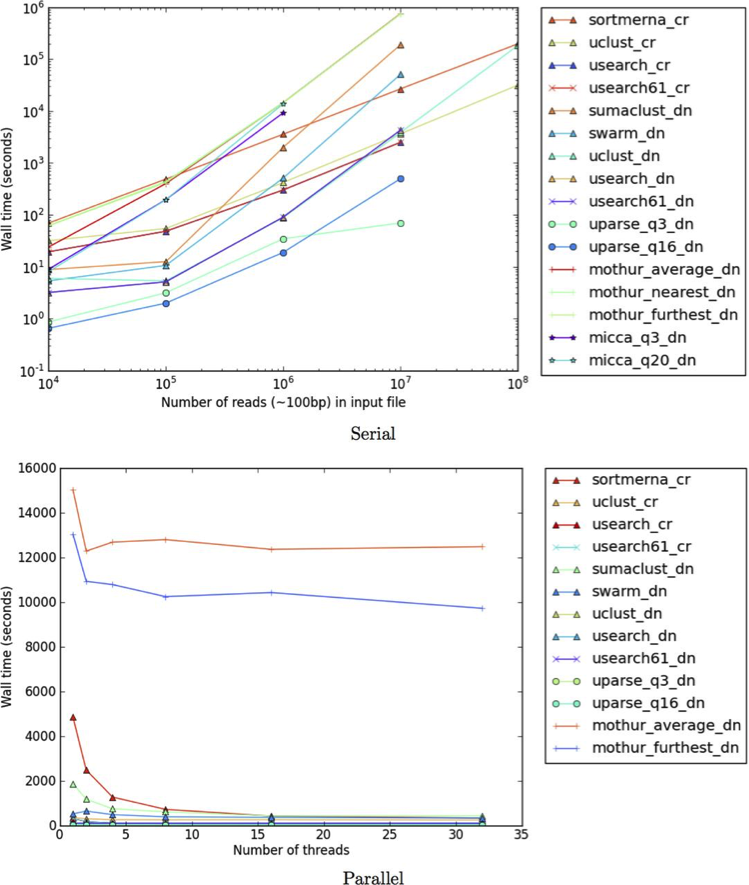
\includegraphics[height=0.55\textheight]{chapter_otupicking_figures/stateArtF5.png}
\end{center}
\caption[Runtime performance of all benchmarked software]{\textbf{Runtime performance of all benchmarked software.}
All tests were performed using 1 to 32 coers on Intel Xeon CPU E5-2640 v3 at 2.60 GHz.
Input files contained reads subsampled from the Global Gut \cite{Yatsunenko2012}.
For serial performance, some tools do not show results for $10^8$ reads due to
exceeding wall time limit (230 hours) or failed memory allocation. For parallel performance,
a single file containing 1 million Illumina sequences was used over multiple threads}
\label{stateArtF5}
\end{figure}

\subsection{Deblur rapidly resolves single-nucleotide community sequence patterns}\label{subsection_deblur}

Sections~\ref{subsection_openref} and~\ref{subsection_soa} were focused on
improving the performance of the \gls{otu} picking process for analyzing
microbial community datasets. \gls{otu}s are defined to approximate the species
richness of a sample, and reduce the effects of the sequencing error from \gls{ngs}
technologies. However, \gls{otu}s are based on an arbitrary sequence identity
threshold (typically 97\%), which reduces the phylogenetic resolution, because two
sequences that are more similar than the identity threshold can't be differentiated.
To assess this problem, we presented a new method, Deblur, that instead of grouping
sequences based on an arbitrary sequence identy threshold, uses statistical
methods to find the underlying true sequence and remove erroneus sequences \cite{Amir2017}.

The following material has been adapted from the original publication in
\textsl{mSystems, 2016}. As a contributor to this manuscript, I was involved in
the discussions of the Deblur pipeline, contributed to the source code, generated
figures for the manuscript and reviewed drafts of the manuscript.

Similar in concept to AmpliconNoise \cite{Quince2011}, a denoising method for
pyrosequencing, Deblur, like DADA2 \cite{Callahan2016} and UNOISE2 \cite{Edgar2016},
attempts to obtain single-nucleotide resolution from Illumina data with
statistical methods to infer the putative true sequences within a sample that
give rise to the distribution of observed error-prone sequences. Unlike DADA2 and
UNOISE2, Deblur operates on each sample independently. It compares
sequence-to-sequence Hamming distances within a sample to an upper-bound error
profile combined with a greedy algorithm to obtain single-nucleotide resolution.
The Deblur algorithm is implemented as follows (see Figure~\ref{figure_deblur}).
First, sequences are sorted by abundance. Second, from the most to least
abundant sequence, the number of predicted error-derived reads is subtracted
from neighboring reads based on their Hamming distance, using an upper bound on
the error probability. A parameterized maximal probability for indels
(defaulting to 0.01) and a parameterized mean read error rate for normalization
(defaulting to 0.5\%) are included. Finally, any sequence whose abundance drops
to 0 after a subtraction is removed from the list of valid sequences. Sequences
not considered to be valid (i.e., noise) are removed. After applying Deblur,
only reads likely to have been presented to the sequencer are retained.
However, it is possible that the reads would still contain chimeras originating
from PCR. Reads are filtered for de novo chimeras using UCHIME \cite{Edgar2011}
as implemented by VSEARCH \cite{Rognes2016} using modified parameters.

\begin{figure}[htbp]
\begin{center}
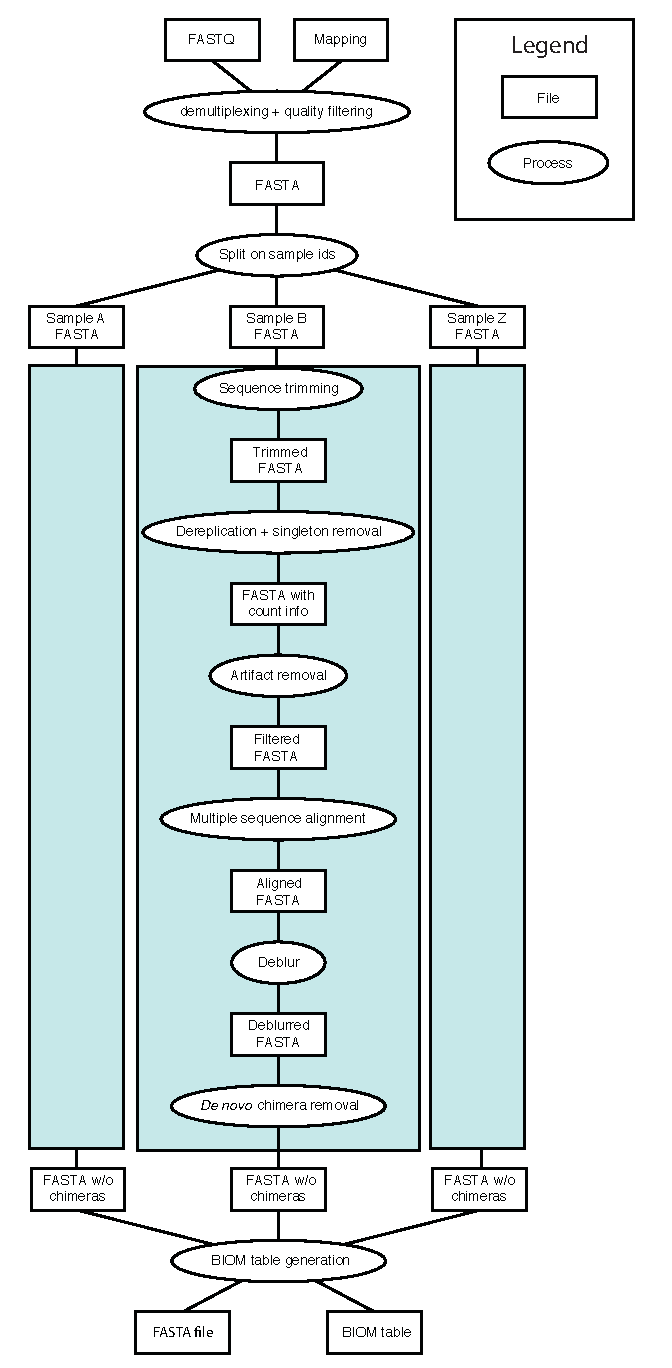
\includegraphics[height=0.70\textheight]{chapter_otupicking_figures/deblurWorkflow.pdf}
\end{center}
\caption[The deblur pipeline]{\textbf{The deblur pipeline.}
A demultiplexed and quality filtered fasta/fastq file (or a directory of per-sample
fasta/fastq files) is used as the input to the pipeline. Following initial
splitting to per-sample fasta files, all processing is done independently on each
sample. Sequences are trimmed and dereplicated with singletons removed. Reads are
then depleted from sequencing artifacts either using a set of known sequencing
artifacts (such as PhiX) (negative filtering) or using a set of known 16S sequences
(positive filtering). Resulting nonartifact reads are then aligned for easy indel
detection. This multiple sequence alignment is then used as the input for the Deblur
algorithm. Each Deblurred sample is then checked for de novo chimeras, and the
resulting s\gls{otu}s from all samples are combined into a single BIOM \cite{McDonald2012BIOM}
table (with sequences labeled as the s\gls{otu} IDs)}
\label{figure_deblur}
\end{figure}

Stability (i.e., obtaining the same s\gls{otu} across different samples) is becoming
critical as more study designs exploit existing samples from resources like the
Earth Microbiome Project \cite{Gilbert2014} or require integration of sequence
data collected over time such as the American Gut Project \footnote{\url{http://americangut.org}}.
We compared the levels of stability of Deblur and DADA2 using technical replicates
from a data set consisting of 40 individuals, each with one fecal sample sequenced
twice on two separate MiSeq runs \cite{Hildebrand2014}. s\gls{otu}s for each run were
assessed separately, and we compared the fractions of s\gls{otu}s from one run to
those present in the second run, as a function of the minimal s\gls{otu} frequency.
Deblur showed greater stability than DADA2 at a higher frequency cutoff (Figure ~\ref{figure_deblur_bench}-A),
indicating that a larger fraction of s\gls{otu}s from the first run were also identified in the second run.

Next, we compared DADA2 and Deblur using a complex natural community and a previously
published data set of fecal samples from two species of howler monkeys \cite{Amato2016}.
Deblur and DADA2 detected 1,938 and 1,636 s\gls{otu}s, respectively, after removal
of s\gls{otu}s with fewer than 10 total reads from each method. Following filtering,
about 70\% of the s\gls{otu}s were identical between the methods. As expected, both
methods identified differential s\gls{otu}s (permutation-based rank mean test;
0.1 false-discovery rate–Benjamini-Hochberg method [FDR-BH] control value) with 61\%
of Deblur s\gls{otu}s differentiating between primate species (1,193/1,938),
compared to 55\% of DADA2 s\gls{otu}s (891/1,636). To assess whether the
s\gls{otu}s unique to either method were from increased numbers of artifacts,
we used \gls{blast} \cite{Altschul1990} to compare each unique sequence against
nt/nr and plotted the fraction of s\gls{otu}s with zero, one, or two mismatches.
We observed that s\gls{otu}s unique to Deblur showed fewer mismatches than those
unique to DADA2 (Figure ~\ref{figure_deblur_bench}-B). The distribution of
s\gls{otu}s over the monkey samples suggests that the s\gls{otu}s unique to Deblur
are more plausible because they show a pattern similar to those identified by both
methods, whereas the s\gls{otu}s unique to DADA2 have markedly different patterns
of clusters of unique s\gls{otu}s within single samples (Figure ~\ref{figure_deblur_bench}-C).

Finally, to explore performance characteristics, we used a MiSeq run from the
stability analysis in order to assess computational space and time demands of DADA2,
Deblur, and UNOISE2 (where possible) over an increasing number of samples.
UNOISE2 was an order of magnitude faster than Deblur, while Deblur was an order of
magnitude faster than DADA2 (Figure ~\ref{figure_deblur_bench}-D).

\begin{figure}[htbp]
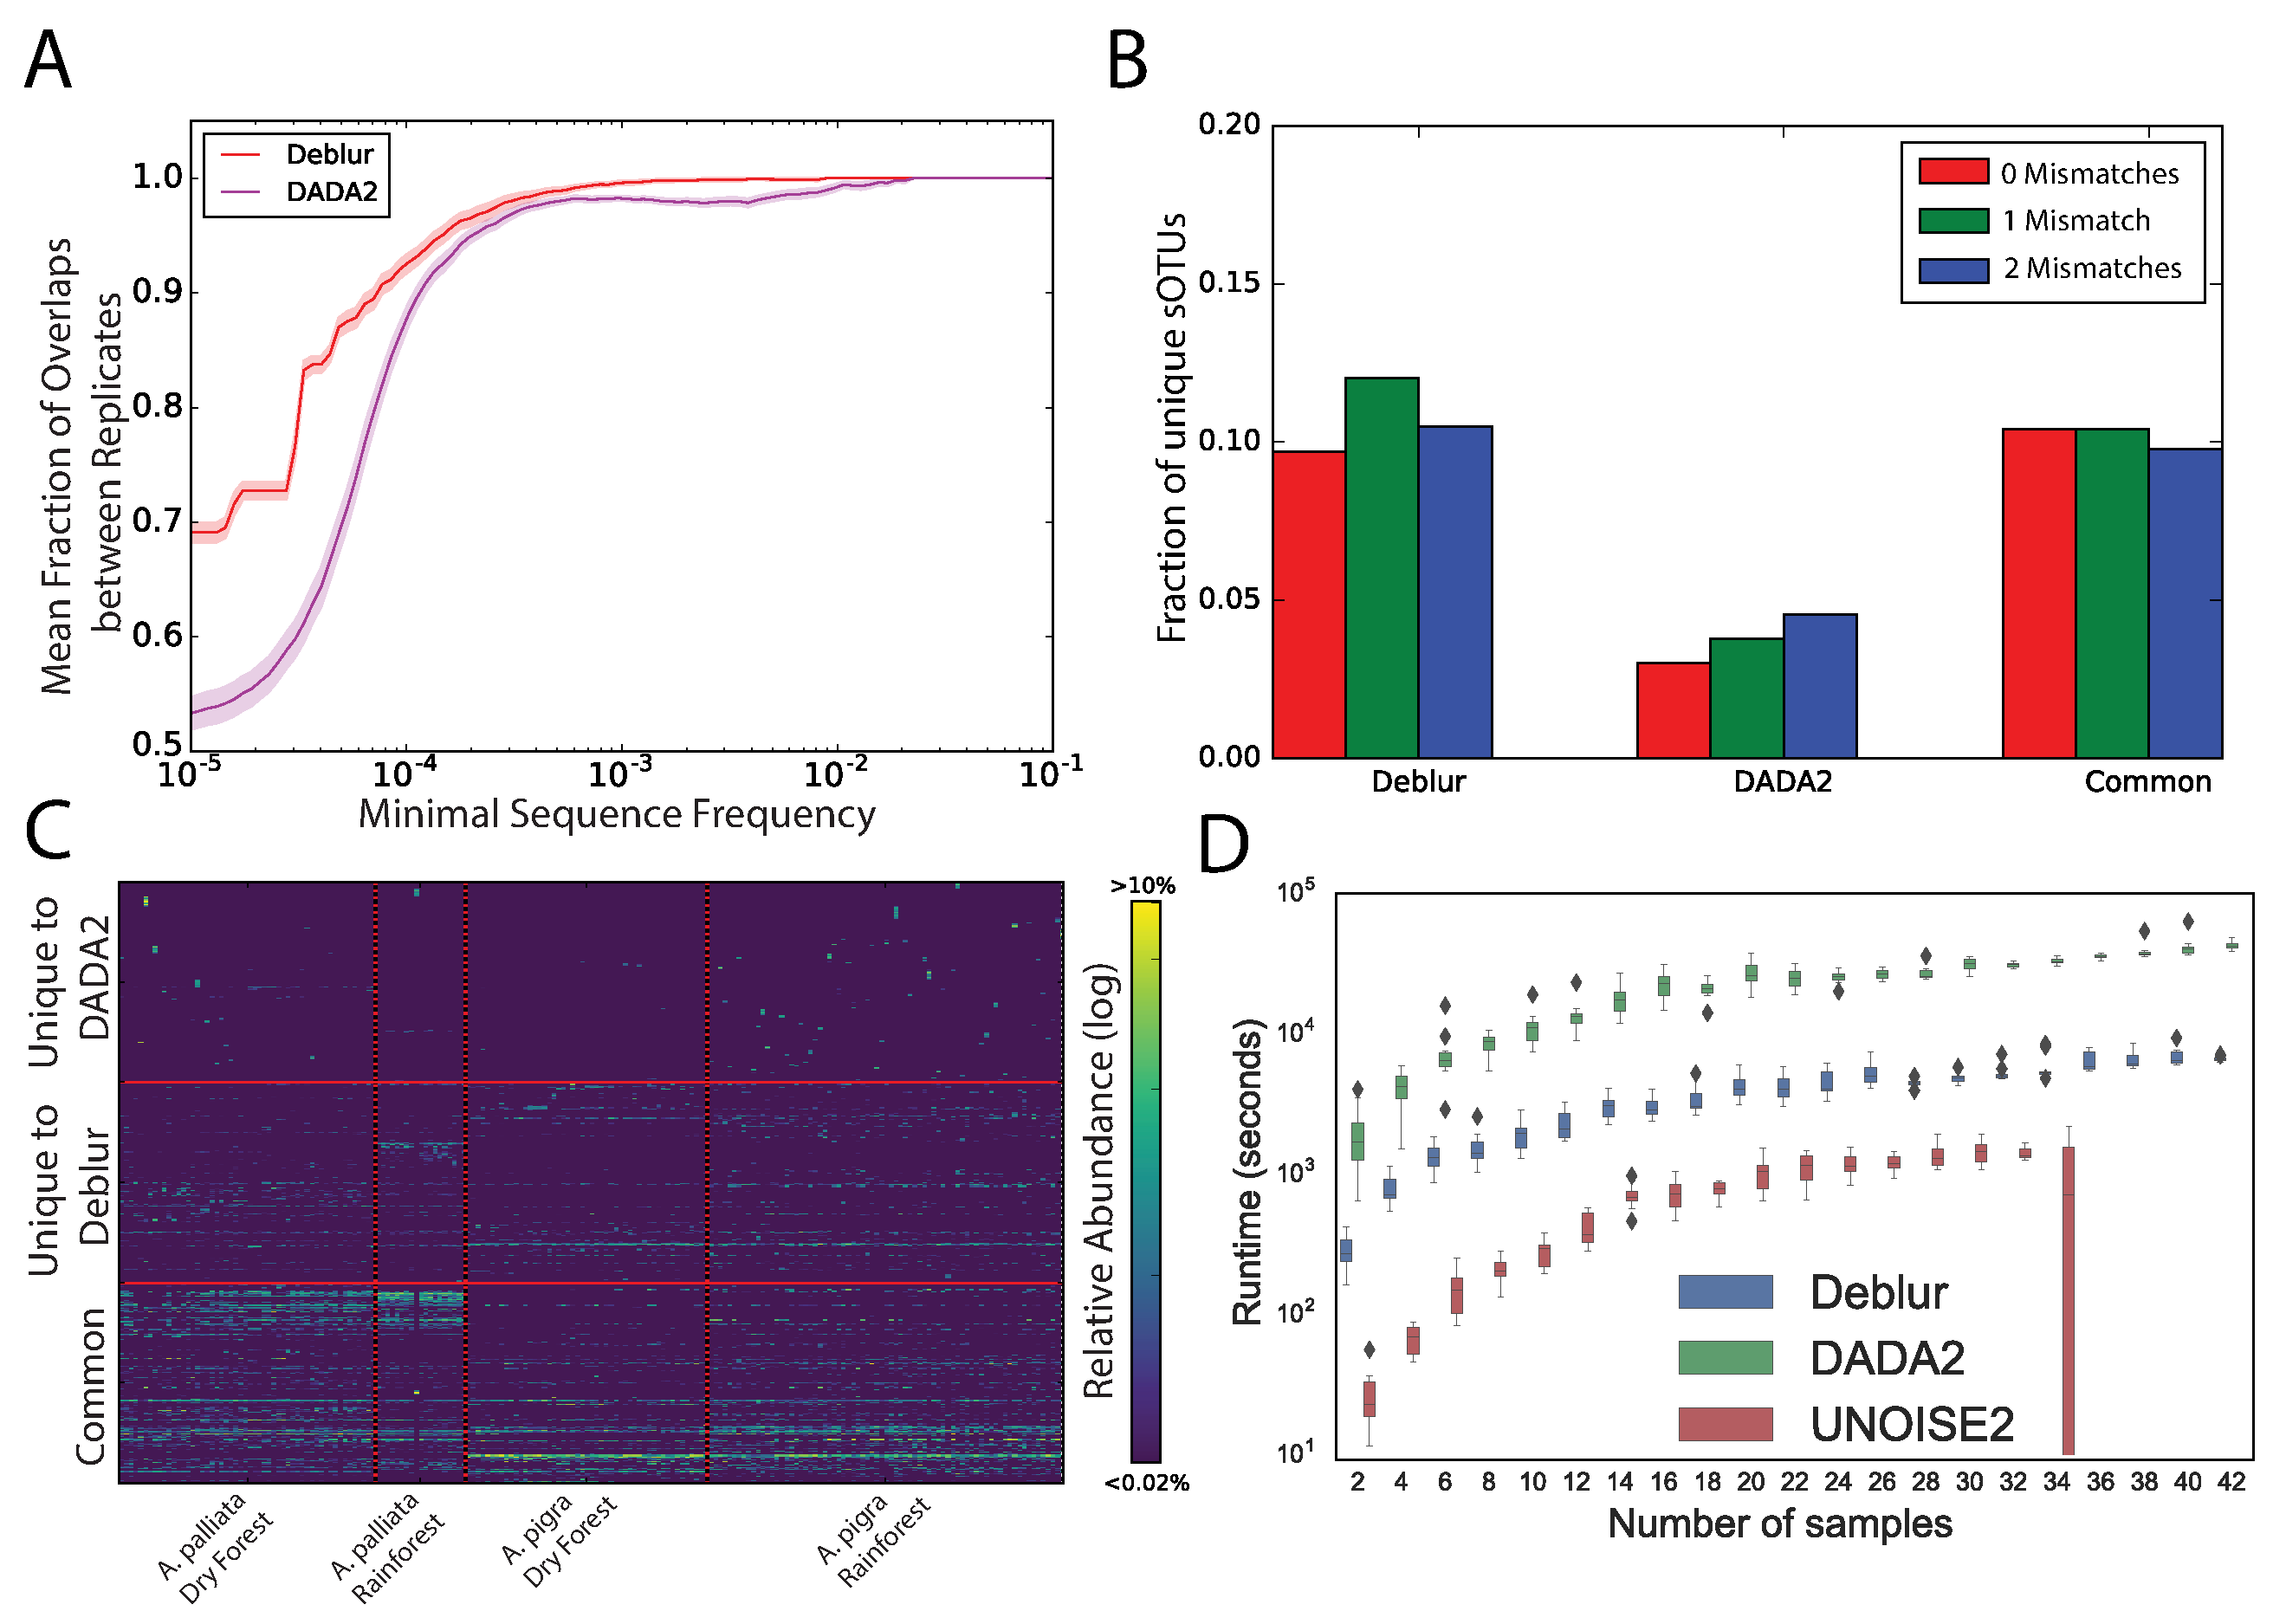
\includegraphics[width=\columnwidth]{chapter_otupicking_figures/deblurBench.pdf}
\caption[Benchmarks of \gls{otu} picking tools on natural communities]{\textbf{Benchmarks of \gls{otu} picking tools on natural communities.}
(A) Stability analysis on experimental technical repeats. Data indicate fractions
of overlapping s\gls{otu}s from two technical replicates in all \gls{otu}s as a
function of the minimal frequency threshold present in one of the repeats.
(B and C) Application of Deblur in the howler monkey data set. (B) Fraction of
sequences matching entries in the \gls{ncbi} nr/nt database
(as of 1 December 2016) with 0.1 or 2 mismatches (red, green, or blue, respectively)
from s\gls{otu}s unique to Deblur or to DADA2 or present in both (left to right).
(C) Heat maps showing s\gls{otu}s (rows) in common with Deblur and DADA2, as well
as those unique to Deblur and DADA2 (bottom, middle, and top rows, respectively).
Samples (columns) are sorted by species and habitat. A total of 200 s\gls{otu}s per group
(i.e., common, unique to Deblur, or unique to DADA2) were randomly selected for
visualization purposes. (D) Single-threaded runtime comparison of Deblur, DADA2,
and UNOISE2 against one of the stability MiSeq runs at increasing numbers of samples.}
\label{figure_deblur_bench}
\end{figure}

\section{Applying these tools to advance microbiome science}\label{section_contributions}

Sections~\ref{section_book} and~\ref{section_bottlenecks} presented my work
on standardizing and improving the pipelines to analyze microbial community data.
Sections~\ref{subsection_komodo},~\ref{subsection_emp},~\ref{subsection_ag}
and~\ref{subsection_bloom} provide examples of manuscripts that I have been
involved in that have taken advantage of my work presented so far.

\subsection{The oral and skin microbiomes of captive Komodo dragons are significantly shared with their habitat}\label{subsection_komodo}

The following text has been adapted from the original publication in
\textsl{mSystems, 16}. As a contributor to this manuscript, I performed the data
analysis included in the manuscript, wrote the IPython notebok \cite{Perez2007}
attached to the publication, generated figures and reviewed drafts of the manuscript.

The evidence for both vertebrate animals and humans indicates that closed
environments not only limit exposure to complex microbial diversity but also
promote microbial transfer from the host to the environment, rather than from
the environment to the host. Fully characterizing the effects of captivity on
host-environment microbial sharing will be key for future studies of vertebrate
microbial ecology and may prove instrumental in improving animal husbandry
practices. To more thoroughly describe the effects of captivity on host-environment
microbiome sharing and how this may affect vertebrate ecology studies, there is a
need to examine the microbial ecology of the host-environment interaction in a
number of vertebrate species, both in the wild and in captivity. Here we use as
a model the captive Komodo dragon (\emph{Varanus komodoensis}), applying 16S \gls{rrna}
amplicon sequencing to characterize the oral, fecal, skin, and environment-associated
microbiomes to answer two main questions: first, is the extent of host-environment
microbiome sharing observed for captive Komodo dragons typical of that observed
among other vertebrates living in closed environments, and second, is the
host-environment microbiome sharing observed among captive Komodo dragons
characteristically different from that observed among wild vertebrates? To
answer these questions, we explored whether host-environment microbiome sharing
in captive Komodo dragons was similar to the pattern observed for humans and pets
living in homes \cite{Lax2014} and dissimilar to the pattern observed among wild amphibians
living in open ecosystems \cite{Kueneman2014}. Together with existing studies, the data suggest that
living in closed environments is associated with extensive host-environment microbial
sharing. This sharing is likely to be circular in nature—the host contributes
microbes to its environment and then, in the absence of significant exposure to
microbes from external sources, reacquires those microbes from its environment,
only to share them with the environment once again (or vice versa). This may be
a radical departure from the microbial communities and exposures which vertebrates
cohabitate with and have evolved alongside in the wild, and could have significant
effects on health and disease \cite{Lax2015}.

To determine how much of the Komodo dragon's microbiome is shared with its environment
(or vice versa) and whether and how specific the environment is to the dragon, we
obtained matched dragon-environment samples from the Denver and Honolulu zoos. In
terms of taxonomic composition and abundance, environmental microbiomes appeared most
similar to salivary and skin microbiomes from the phylum down to the genus level
in both the Denver and Honolulu zoo cohorts (see Figure~\ref{KomodoST} A).

We applied SourceTracker \cite{Knights2011} to samples from the Denver Zoo Komodo
dragons to determine which dragon microbiome sources (saliva, feces, and skin)
contributed to the dragon environment. The microbiomes of items in the Denver
Komodo dragons’ enclosures were largely sourced from Komodo dragon salivary, skin,
and fecal samples (Figure~\ref{KomodoST} B), with unknown sources comprising less
than 50\% of the microbial communities of most environmental sample types.
Additionally, skin, saliva, and fecal communities were distinct from one another
in a SourceTracker independence test (Figure~\ref{KomodoST} B), suggesting that
any skin, saliva, or fecal communities detected on environmental materials actually
came from the dragon’s skin, mouth, or feces. Further supporting this point—at
least in the context of saliva—several bacterial taxa found in the mouths of the
Komodo dragons studied here, including \emph{Staphylococcus}, \emph{Corynebacterium},
\emph{Pseudomonas}, and \emph{Bacteroides}, have previously been reported in the
mouths of captive Komodo dragons \cite{Montgomery2002, Goldstein2013}. This
suggests that environmental microbes designated as sourced from the Komodo dragon’s
oral cavity likely actually do come from the mouth and not any other source. The
nature and extent of host-microbiome transfer to environmental objects varied with
sample type; for example, Komodo dragon saliva was the main source of the microbial
communities detected in soil and on rock and glass, while Komodo dragon skin was
the main source of the microbial communities detected on metal (Figure~\ref{KomodoST} B).
Performing SourceTracker analyses with Komodo dragon samples designated as sinks
and environmental samples designated as sources revealed that the microbial
communities of Komodo dragon fecal, saliva, and skin samples are sourced from a
variety of environmental materials, each contributing 30\% or less of the microbial community
(Figure~\ref{KomodoST} C and D). There is no one environmental material that contributes
more than any other material to Komodo dragon feces or saliva; however, Komodo skin microbial
communities are sourced majorly from glass and unknown sources (each ~40\%).

\begin{figure}[htbp]
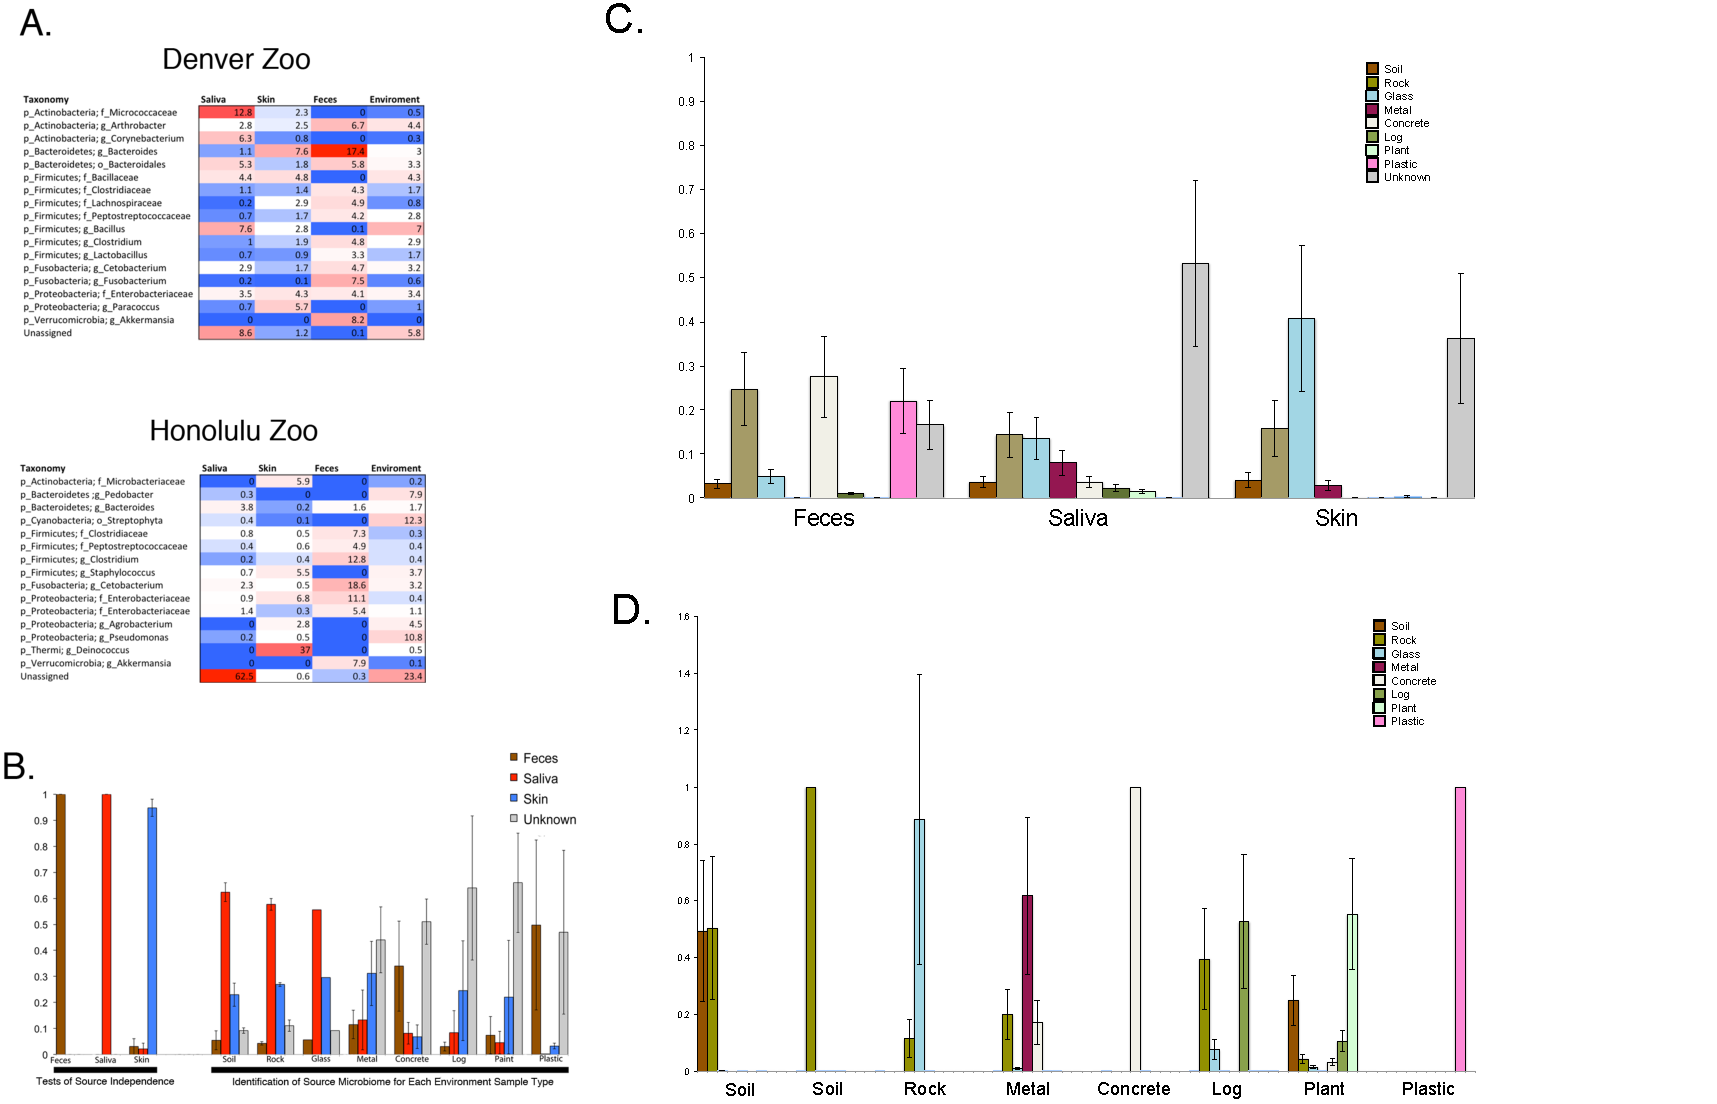
\includegraphics[width=1.15\columnwidth]{chapter_contributions_figures/KomodoSTest.pdf}
\caption[Taxonomy and SourceTracker results for the Komodo dataset]{\textbf{Taxonomy and SourceTracker results for the Komodo dataset.}
(A) Heat maps illustrate the percent abundances of the most abundant genera
(all \gls{otu}s taxonomically classified to the same genus were collapsed into
a single genus summary) present in saliva, skin, feces, and environmental (Env)
samples collected from the Denver and Honolulu zoos. The deepest taxonomic
classification achieved is listed for each genus. The heat map colors indicate
percent abundance (red [high abundance] to blue [low abundance]). (B) Komodo
dragon SourceTracker analysis reveals that the microbial communities of many
environmental sample types are sourced from skin, saliva, and feces rather than
unknown sources (i.e., not from Komodo dragon skin, saliva, or feces). Data are
plotted as the means $\pm$ standard errors of the means (error bars) of samples
from Denver and Honolulu zoo Komodo dragons. (C) SourceTracker analyses with
Komodo dragon fecal, salivary, and skin samples designated as sinks and environmental
samples designated as sources reveals that a variety of environmental sources,
rather than a single environmental source, contribute to the microbial communities
of Komodo dragon feces, saliva, and skin. Unknown sources (i.e., not the environments
sampled from the Komodo dragon enclosures) also contribute about 40\% or more of
the microbial community of saliva and skin samples (only 20\% of fecal samples).
(D) Independence tests reveal that about half of the environmental samples are not
independent from other environmental samples. Data are the means $\pm$ standard errors
of the means of Denver and Honolulu Komodo dragon and environmental samples.}
\label{KomodoST}
\end{figure}

To further assess host-environment microbiome sharing, in both closed/captive and
open/wild environments, we additionally performed SourceTracker analyses on two
previously published data sets—a wild amphibian skin-environment microbiome data set
\cite{Kueneman2014} and a human-pet-house microbiome data set \cite{Lax2014}—and
compared them to the Komodo dragon data set. As previously shown, humans and their
pets contribute a large amount of their microbiomes to their living environments
\cite{Lax2014}, similarly to the patterns we observed with captive Komodo dragons.
However, while Komodo dragon microbiome sources (skin, saliva, and feces) were
found to be distinct sources, we did not observe this level of source independence
when applying the SourceTracker independence test to the human/pet data set.

Host-environment microbiome sharing between amphibians and their living environment
was not as extensive as that observed among captive Komodo dragons and their
enclosures or humans and pets and their homes. More than 75\% of soil and sediment
microbial communities were obtained from unknown microbiome sources; however,
the identified “source” for 75\% of water microbial communities was amphibian skin
(Figure ~\ref{AmphibianST} A). Each source (here defined as individual amphibian
species) was highly independent from each other source (Figure ~\ref{AmphibianST} B).
Defining amphibian skin as a sink and environmental samples as sources, water was
identified as a major source of the microbes on the skin of most species; nevertheless,
at least 20\% of the microbial community on the skin of all species was contributed
by unknown sources (Figure ~\ref{AmphibianST} C). Soil, sediment, and water were
all confirmed to be independent sources (Figure ~\ref{AmphibianST} D).

\begin{figure}[htbp]
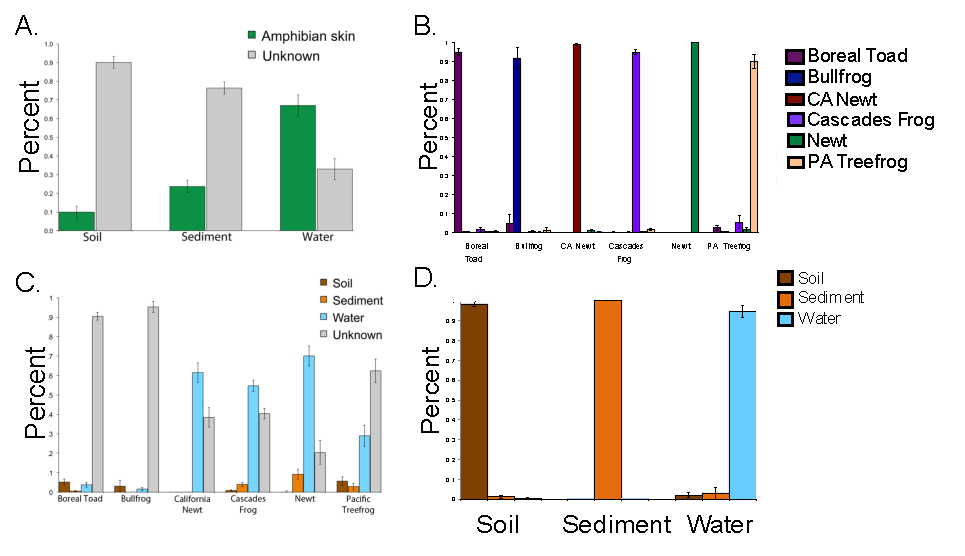
\includegraphics[width=\columnwidth]{chapter_contributions_figures/AmphibiansST.pdf}
\caption[SourceTracker results for the amphibians dataset]{\textbf{SourceTracker results for the amphibians dataset.}
(A) Amphibian SourceTracker analysis reveals that water is the only sample type
that obtains a notable amount of its microbial community from amphibian skin; unknown sources
(i.e., not amphibian skin) are the main microbiome contributors to soil and sediment.
(B) Independence tests reveal that amphibian skin is independently specific to species.
(C) Designating environment the source and amphibian skin the sink reveals that water
is the only environmental type that contributes largely to the microbial communities
on amphibian skin, with unknown sources also largely contributing to the amphibian
skin microbiome. (D) Independence tests reveal that each environment type is also
independent from each other environment type. Data are the means $\pm$ standard
errors of the means.}
\label{AmphibianST}
\end{figure}

\subsection{A communal catalogue reveals Earth's multiscale microbial diversity}\label{subsection_emp}

The following material has been adapted from the original publication in
\textsl{Nature, 2017}. As a contributor to this manuscript, I quality filtered the
97 independent studies included in the manuscript, generated the \gls{otu}-based
closed and open reference tables and the open reference phylogenetic tree and provided
scripts to reproduce those steps.

The \gls{emp} was founded in 2010 to sample the Earth's microbial communities at an
unprecedented scale in order to advance our understanding of the organizing
biogeographic principles that govern microbial community structure
\cite{Gilbert2010, Gilbert2014, Thompson2017}. The \gls{emp} asked the global scientific
community for environmental samples and associated metadata spanning diverse
environments and capturing spatial, temporal, and/or physicochemical covariation.
The first 27,751 samples from 97 independent studies represent diverse environment
types (Figure ~\ref{EMProvenance} A), geographies (Figure ~\ref{EMProvenance} B),
and chemistries. The \gls{emp} encompasses studies of bacterial, archaeal, and
eukaryotic microbial diversity. The analysis here focuses exclusively on the
bacterial and archaeal components of the overall database (for concision, use of
‘microbial’ will hereafter refer to bacteria and archaea only). Associated metadata
included environment type, location information, host taxonomy (if relevant), and
physicochemical measurements. Physicochemical measurements were made in situ at
the time of sampling. Investigators were encouraged to measure temperature and
pH at minimum. Salinity, oxygen, and inorganic nutrients were measured when possible,
and investigators collected additional metadata pertinent to their particular investigations.

\begin{figure}[htbp]
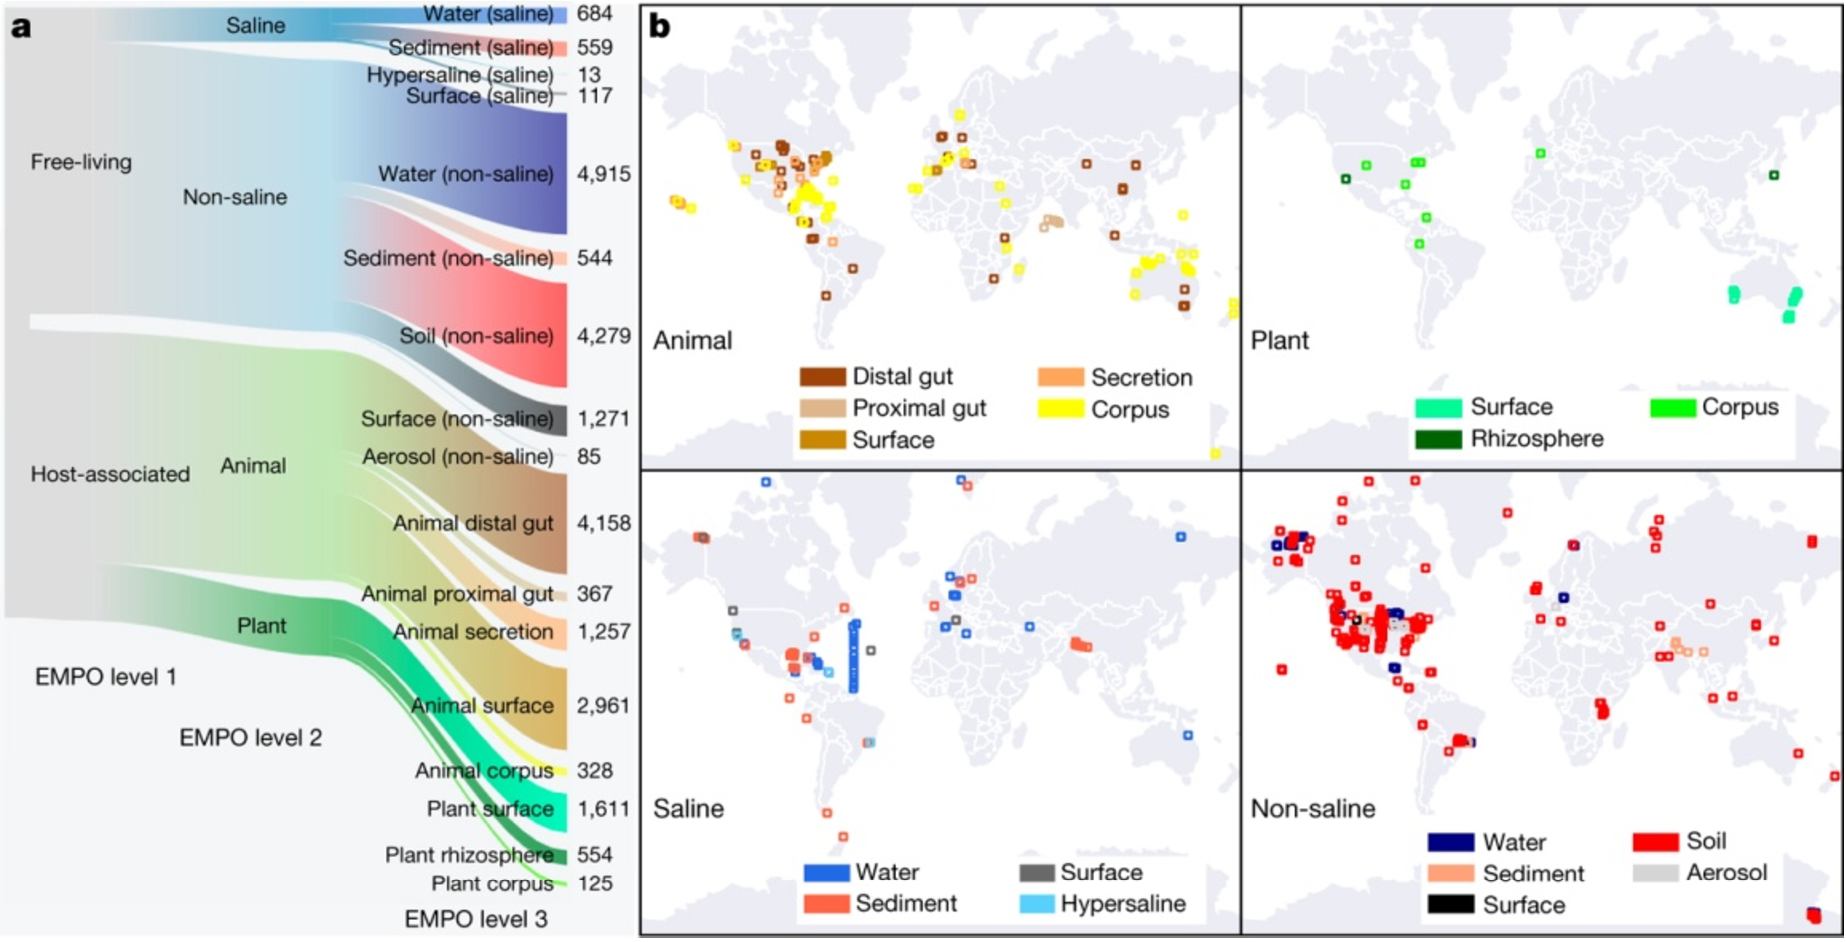
\includegraphics[width=\columnwidth]{chapter_contributions_figures/EMProvenance.pdf}
\caption[Environment type and provenance of samples]{\textbf{Environment type and provenance of samples.}
(A) The \gls{empo} classifies microbial environments (level 3) as free-living or
host-associated (level 1) and saline or non-saline (if free-living) or animal
or plant (if host-associated) (level 2). The number out of 23,828 samples in the
QC-filtered subset in each environment is provided. \gls{empo} is described with examples
at http://www.earthmicrobiome.org/protocols-and-standards/empo. (B) Global scope of
sample provenance: samples come from 7 continents, 43 countries, 21 biomes (\gls{envo}),
92 environmental features (\gls{envo}), and 17 environments (\gls{empo}).}
\label{EMProvenance}
\end{figure}

Beyond measured physical covariates, the breadth of environments in the \gls{emp}
catalogue allows a detailed exploration of how microbial diversity is distributed
across environments. Diversity among communities (beta-diversity) is driven by
turnover (replacement of taxa) and nestedness (gain or loss of taxa resulting in
differences in richness) \cite{Carvalho2013}. If turnover dominates, then
disparate communities will harbour unique taxa. If nestedness dominates, then
communities with fewer taxa will be subsets of communities with more taxa. We
tested for nestedness using a 2,000-sample subset with even representation across
environments and studies. Given the contrasting environments and geographic separation
among the many studies in the \gls{emp}, we expected different environments to
contain unique sets of taxa and to show little nestedness. However, we found that
communities across environments were significantly nested (Figure ~\ref{EMPNestedness} A, B; P < 0.05)
in comparison to null models (Figure ~\ref{EMPNestedness} C), accounting for the
observed patterns of richness. At coarse taxonomic levels, an average of 84\% of phyla,
73\% of classes, and 58\% of orders that occurred in less diverse samples also
occurred in more diverse samples. These patterns could have resulted from several
mechanisms, including ordered extinctions \cite{Sonnenburg2016} and the filtering
of complex communities over time \cite{Atmar1993}, differential dispersal
abilities \cite{Lomolino1996} and cascading source–sink colonization processes
that assemble nested subsets from more complex communities, or by the tendency
of larger habitat patches to support more rare taxa with lower prevalence \cite{Gaston2000}.
Notably, finer taxonomic groupings showed less nestedness (Figure ~\ref{EMPNestedness} C),
indicating that the processes that underlie nested patterns of turnover are
likely to reflect conserved aspects of microbial biology, and not to result from
the interplay of diversification and dispersal on short timescales.

\begin{figure}[htbp]
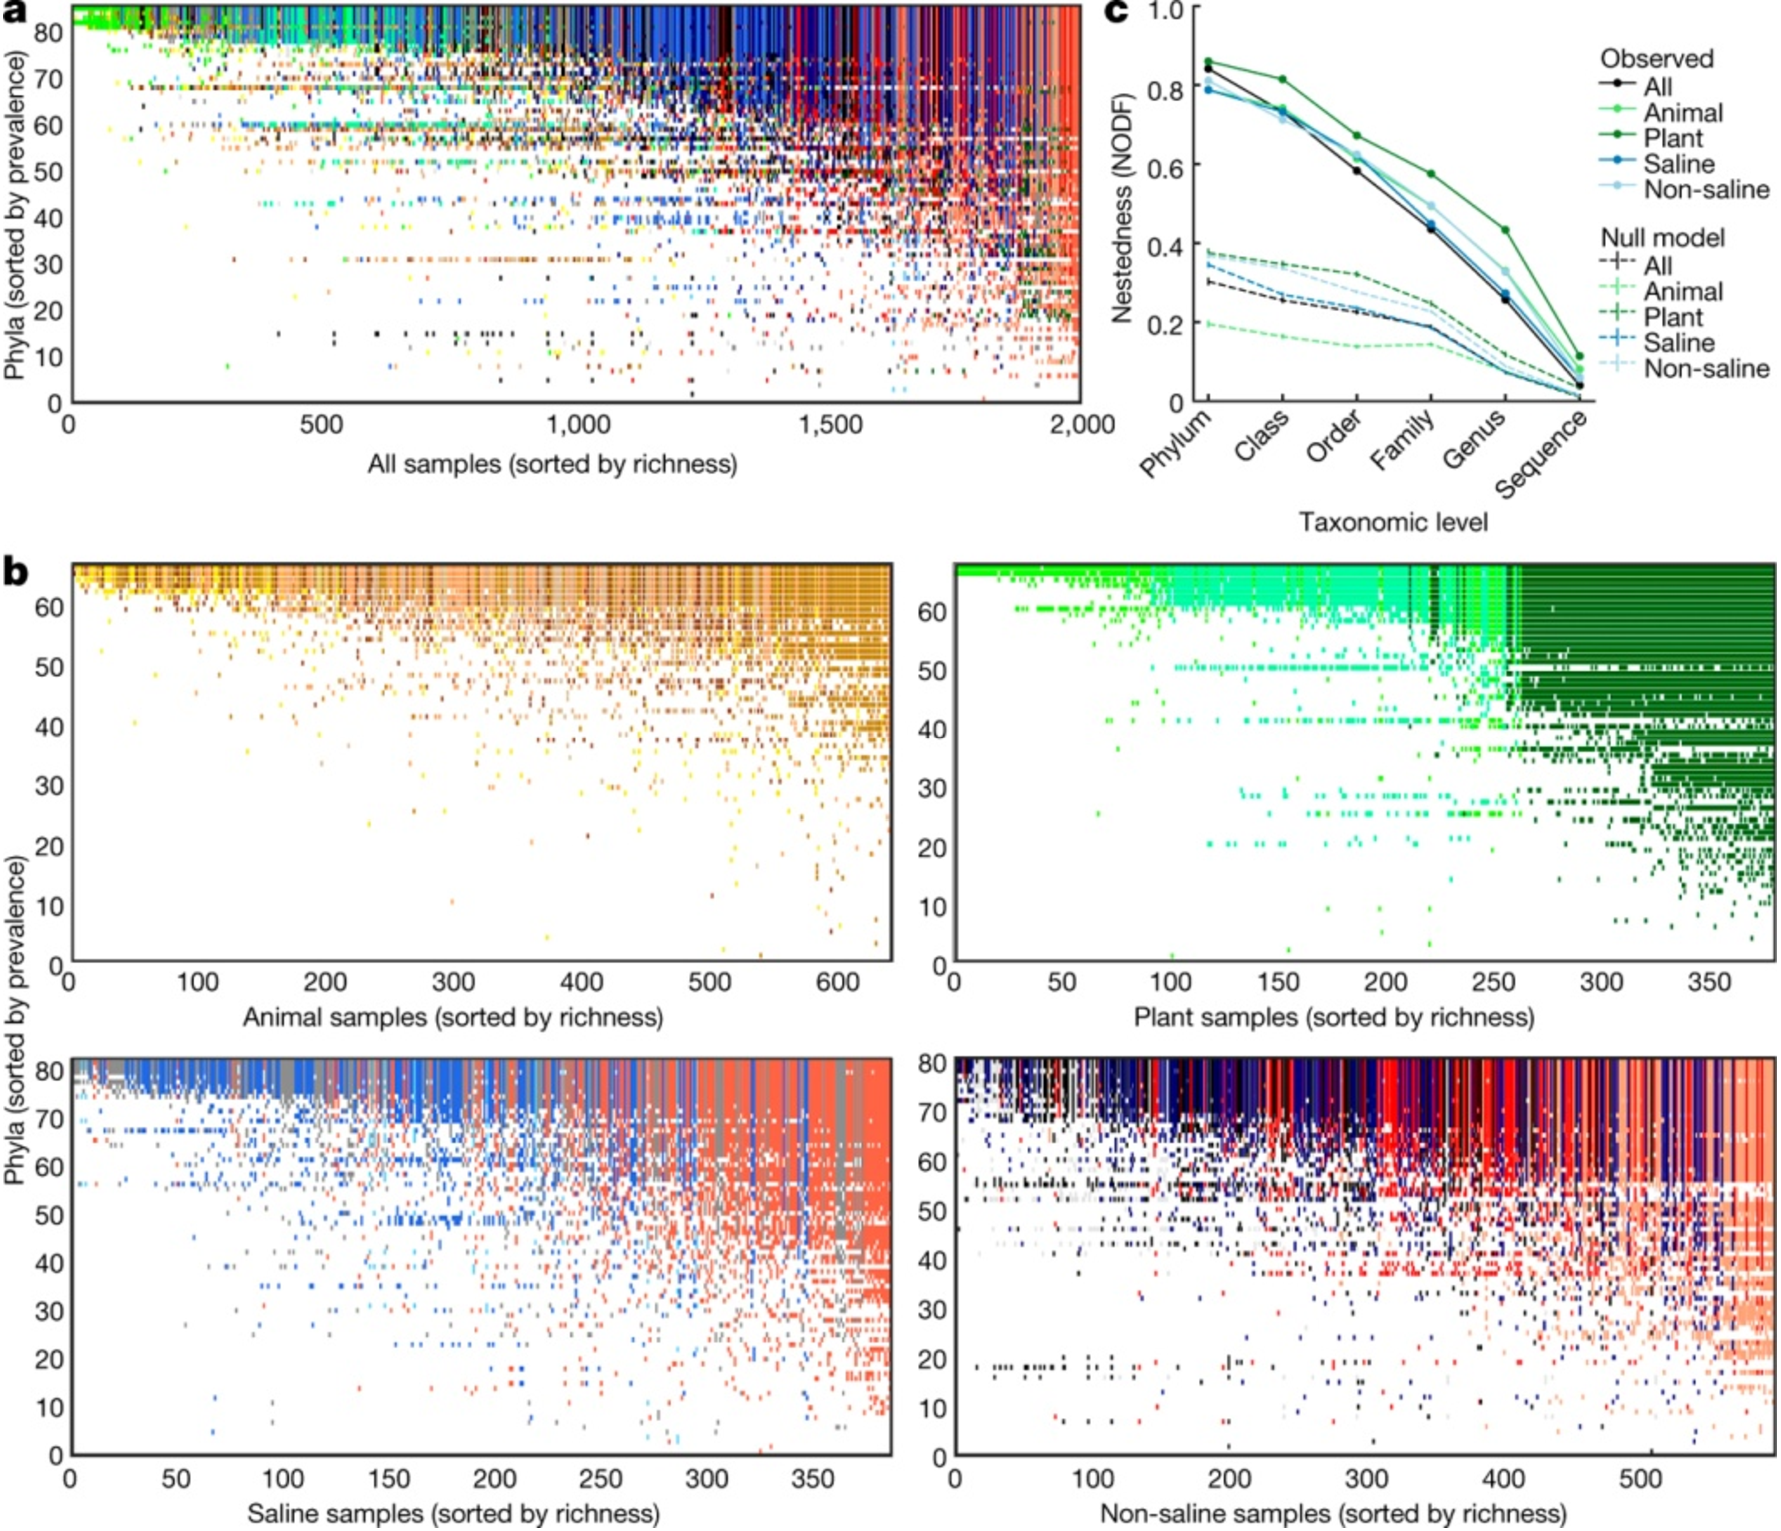
\includegraphics[width=\columnwidth]{chapter_contributions_figures/EMPNestedness.pdf}
\caption[Nestedness of community composition]{\textbf{Nestedness of community composition.}
(A) Presence–absence of phyla across samples, with phyla (rows) sorted by prevalence and samples
(columns) sorted by richness. Shown is a subset of the \gls{emp} consisting of n = 2,000
biologically independent samples with even representation across environments and studies.
With increasing sample richness (left to right), phyla tended to be gained but not lost
(P < 0.0001 versus null model; NODF (nestedness measure based on overlap and decreasing fills)
statistic and 95\% confidence interval = 0.841 $\pm$ 0.018). (B) As in A but separated into
non-saline, saline, animal, and plant environments (P < 0.0001, respective NODF = 0.811
$\pm$ 0.013, 0.787 $\pm$ 0.015, 0.788 $\pm$ 0.018 and 0.860 $\pm$ 0.021). (C) Nestedness as
a function of taxonomic level, from phylum to tag sequence, across all samples and within
environment types. Also shown are median null model NODF scores ($\pm$ s.d.).
NODF measures the average fraction of taxa from less diverse communities that occur in
more diverse communities. All environments at all taxonomic levels were more nested than
expected randomly, with nestedness higher at higher taxonomic levels (for example, phyla).}
\label{EMPNestedness}
\end{figure}

\subsection{American Gut: An open platform for citizen-science microbiome research}\label{subsection_ag}
The following material has been adapted from the original publication submitted in
\textsl{Science, 2018}. As a contributor to this manuscript, I generated the per
participant results, provided support maintaining the software and reviewed drafts
of the manuscript.

We therefore launched the \gls{agp} \footnote{\url{http://americangut.org}}, now the
largest crowdfunded and crowdsourced microbiome citizen-science project to date,
with the goal to discover the kinds of microbes and microbiomes "in the wild.”
Our project informs participants about their own microbiomes by providing them with
a standard report that places them in context of the full AGP and Human Microbiome
Project (HMP) datasets, and provides a broad set of resources to support research
about the human microbiome, including an online course. Unlike many other large
microbiome studies, the AGP deposits all de-identified data into the public domain
on an ongoing basis without access restrictions. This reference database has allowed
us to characterize the diversity of the industrialized human gut microbiome at an
unprecedented scale, to explore novel relationships with health, lifestyle, and
dietary factors, and to establish the AGP resource and infrastructure as a living
platform for discovery (e.g., through targeted sub-populations and through the
application of multi-omics techniques).

Key variables that we found to have the greatest effects on the composition of gut
microbes - plant consumption, antibiotic use, and even age - are in flux in the global
population. Our lifespans are increasing, we are traveling more, our diets are
becoming homogenized, and we are consuming more antibiotics. In each case, these
trends are likely to favor more homogenization and less diverse gut microbes.
Ongoing efforts, such as the AGP, will allow researchers to document and potentially
mitigate the effects of such change. They will also afford insights into our past
through collections from more diverse subpopulations, which will allow us to better
understand the context of our choices in the future.

A unique aspect of the AGP is the open community process of assembling the Research
Network and analyzing these data. Because participants fund the project, no funding
agency mandates restrictions on data analysis to a specific group of investigators.
Thus, these data are released into the International Nucleotide Sequence Database
Collaboration (INSDC) (and GNPS for metabolomics data) as soon as initial quality
control and anonymization steps have been applied. Analysis details are shared
through a public forum \footnote{GitHub, \url{https://github.com/knightlab-analyses/american-gut-analyses}}.
Scientific contributions to the project were made through a geographically diverse
Research Network represented herein as the American Gut Consortium (including explicitly
named authors). This network was established prior to project launch and has continued
to grow over time. The analyses described were performed through an open contribution
model in which pre-computed forms of these data were publicly provided with encouragement
to the American Gut Consortium to explore the dataset. This model allows the project to
use a “living analysis” approach, embracing new researchers and analytical tools on an
ongoing basis (e.g., Qiita and Global Natural Products Social Molecular Networking (GNPS)).
Additionally, because the AGP is a subproject of the Earth Microbiome Project (EMP) \cite{Thompson2017}),
all samples were processed using the publicly available and widely used EMP 16S rRNA gene
amplification, sequencing, and data analysis protocols to facilitate meta-analyses. For
example, we combined the AGP with fecal samples collected from a fecal transplant
study and an infant microbiome time series, the latter using different DNA sequencing
technology, to highlight how this context can provide insight.


\subsection{Correcting for microbial blooms in fecal samples during room-temperature shipping}\label{subsection_bloom}
The following material has been adapted from the original publication in
\textsl{mSystems, 2016}. As a contributor to this manuscript, I was involved in
the discussion for establishing the criteria to choose blooming bacteria, provided
input on the figures design and reviewed drafts of the manuscript.

The use of sterile swabs is a convenient way to collect samples for microbiome studies,
but in some cases, it is not feasible to immediately freeze or utilize a preservative.
For example, the \gls{agp} allows members of the general public to send samples for 16S
\gls{rrna} gene amplicon sequencing through domestic post without a preservative.
This is because proven preservation methods can be cumbersome, dangerous, expensive,
or sample type specific, complicating participation in microbiome citizen science.
Although some studies have demonstrated that the effects of room-temperature storage
are secondary to physiologically relevant differences between comparison groups
\cite{Song2016, Sinha2016, Lauber2010}, certain bacterial taxa,
particularly those in the class \emph{Gammaproteobacteria}, grow well at room temperature.
This is problematic, as some \emph{Gammaproteobacteria} species have been associated
with disease, such as \gls{ibd} \cite{Gevers2014}. Therefore, to identify meaningful
patterns in microbiome studies that do not utilize sample preservation, it is crucial
to remove at high specificity the taxa that thrive at room temperature (i.e., “blooming” bacteria).

Without filtering candidate blooms, there were notable differences (as observed using Bray-Curtis
\gls{pcoa}) between \gls{agp} fecal samples and the fresh-frozen fecal samples;
filtering the bloom sequences from all samples removed these differences (Figure ~\ref{bloomFig} A versus B).
In the \gls{pcoa} space corresponding to the data determined without filtering, the primary
separation is explained by the presence of a large percentage of bloom sequences (Figure ~\ref{bloomFig} A);
the sizes of the spheres are scaled by the percentage of bloom sequences in the respective sample.
Following the removal of the blooms, this dominant effect was abolished and samples with high levels of
blooms clustered with samples from the other studies (Figure ~\ref{bloomFig} B). Similar results were observed
in assessing class-level taxonomy abundances (Figure ~\ref{bloomFig} C versus D): prior to filtering,
a high relative abundance of \emph{Gammaproteobacteria} (27\%) was present in the \gls{agp} samples
compared to the fresh-frozen samples (1.5\% to 3.5\%), while the \gls{agp} profile seen after filtering
more closely resembled that of the fresh-frozen samples. Importantly, applying the filter minimally
changed the taxonomic profiles of fresh-frozen samples (Figure ~\ref{bloomFig} D). The filtering
procedure is available in a Jupyter Notebook \cite{Perez2007} at https://github.com/knightlab-analyses/bloom-analyses.

There is a balance between type 1 and type 2 errors that must be considered in applying this filter.
The cost of removing a sequence is that it becomes “invisible” in the analysis, and it is possible
that real sequences are lost. Conversely, retaining a bloom sequence increases noise caused by shipment
conditions, which can artificially alter biological conclusions. Therefore, a balance between loss of data
and inaccurate, noisy data must be obtained. To select an appropriate number of blooming bacterial
sequences to subtract from the \gls{agp} data set to maximize the amount of data retained while
reducing inaccuracies caused by blooms, we tested the effect of nested filtering levels on the ability
to detect the well-known effect of age on alpha diversity \cite{Yatsunenko2012, Koenig2011}.
As can be seen in Figure ~\ref{bloomFig} E and F,
this effect was undetected by a Kruskal-Wallis test when none of the candidate blooms were removed.
However, filtering the top four candidate blooms restored the ability to detect a significant
difference in diversity by age. Critically, the identification of the bloom sOTUs was done
independently of this positive control. For analysis of the \gls{agp} cohort, we recommend
removal of the sequences of the top 10 candidate blooming bacterial taxa, as this maximizes the expected
age effect (Figure ~\ref{bloomFig} E). Different studies may need to remove a different subset of
bloom sequences, as retaining some of these sequences might be critical, depending on the study
characteristics. With meta-analysis, if this filter is applied, it must be applied identically to
all samples represented to avoid introduction of a systematic bias.

\begin{figure}[htbp]
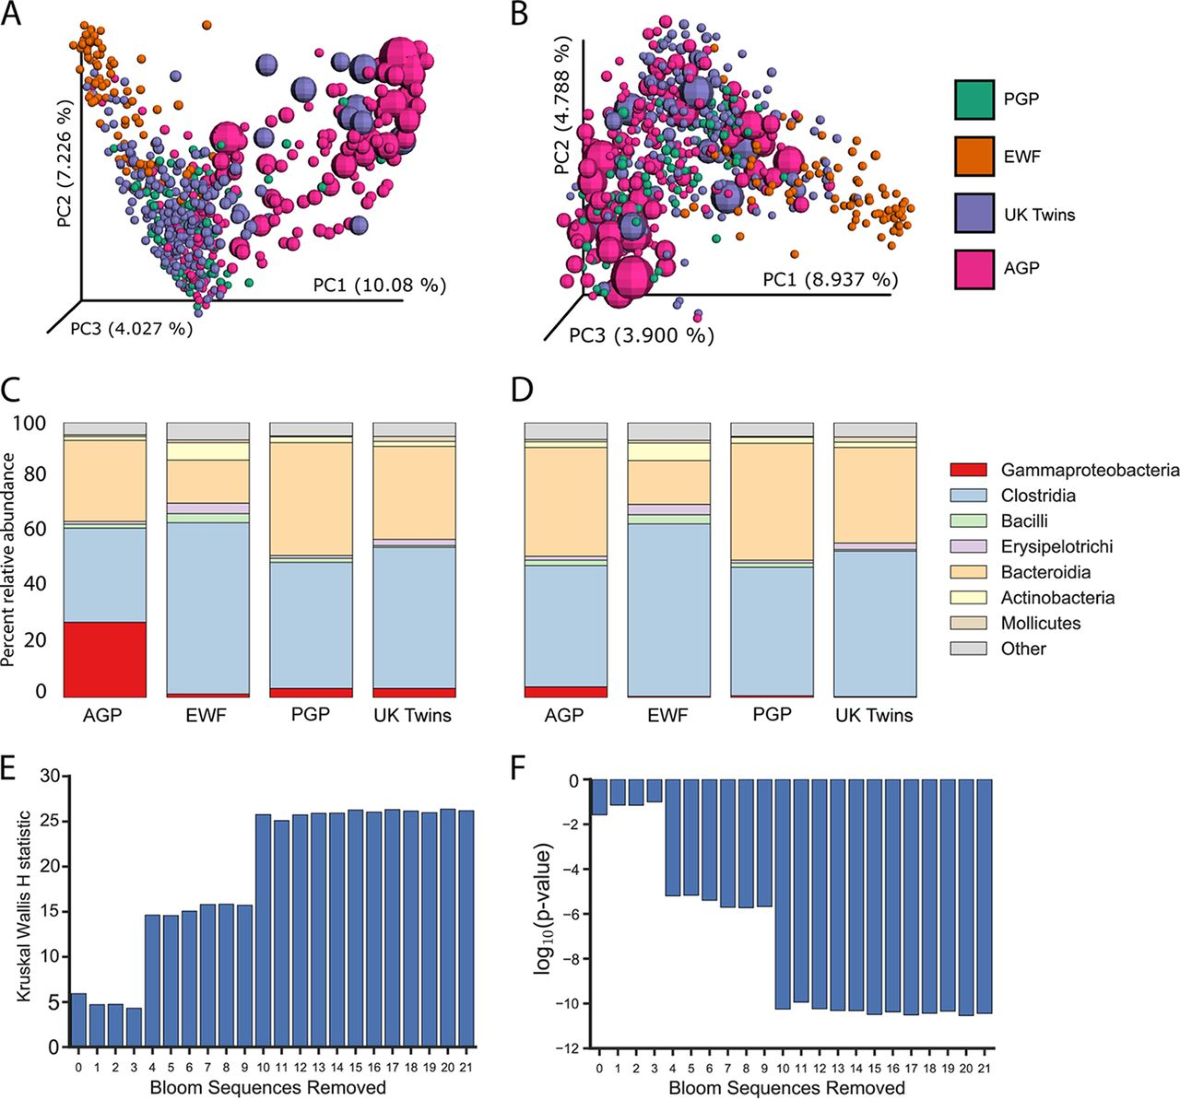
\includegraphics[width=\columnwidth]{chapter_contributions_figures/bloom.pdf}
\caption[Effect of bloom filtering on American Gut data]{\textbf{Effect of bloom filtering on American Gut data.}
(A and B) \gls{pcoa} of Bray-Curtis distances from a random subset of 200 American Gut Project samples (colored pink)
compared to 3 studies containing fresh-frozen fecal samples: Personal Genome Project (colored green);
whole-grain feces \cite{Vitaglione2015} (colored orange); and UK Twins \cite{Goodrich2017} (colored purple), respectively.
The \gls{pcoa} data shown represent results obtained before (A) and after (B) applying the
filter for blooms to all samples. The size of a sphere is scaled by the amount of
candidate bloom bacteria in a sample prior to filtering. (C and D) Mean taxonomy distribution for the
same studies before (C) and after (D) filtering for blooms. (E and F) The well-known effect of age on
alpha diversity and how the effect is observed only after the removal of bloom reads.
The Kruskal-Wallis test statistic (E) and corresponding –log(P value) (F) are shown for
different numbers of bacteria used for the filtering before applying the test. A value of 0 on the
x axis indicates no filtering. The x axis is ordered by decreasing severity score of the bloom where bloom
1 represents greater severity than bloom 2, and each point on the x axis includes the prior blooms
(e.g., position 5 includes bloom sOTUs 1 through 5).}
\label{bloomFig}
\end{figure}


\chapter{Better memory management in the cloud}\label{chapter_cudswap}
\glsresetall

Chapter~\ref{chapter_book} described the first gold standard for analyzing microbial
community datasets, exposed and alleviated some of the computational bottlenecks in the
pipeline and showed some examples of the application of such pipeline. Some of the
steps of the presented pipeline are too computationally expensive to be run in a
personal laptop, and access to a supercomputer is needed to complete those steps.
However, microbiologists do not necessarily have access to supercomputers and they have
to rely on cloud computing. Tools such \gls{qiime} \cite{Caporaso2010} and IPython
\cite{Perez2007} provide \gls{ami}s that enable biologists to run their analysis in
Amazon's \gls{ec2} infrastructure \cite{RaganKelley2013}. This facilitates microbial
biologists' work by avoiding the often complex task of installing the required software to run
their analyses as well as providing an environment suitable to support the large
datasets that then currently face. But running these analyses in the cloud presents
new challenges to microbiologists. One of the first decisions that microbial
biologists face when running these analyses in the cloud is choosing the resources
that their virtual machine in the cloud should contain. Usually microbiologists
are unaware of the resources required by the analysis tools that they are going to
use, and often the requirements of these tools is highly dependant on the nature
of the data. In these cases, the biologists are left with a trial and error procedure
until they have enough resources for their analysis or they have to choose a virtual
machine with more resources than needed that they go underutilized. In both of these
cases, the microbiologists end up spending more money (and time) than
needed, which can be critical for those scientists running on a budget.

Sections~\ref{section_memory_exhaustion} and~\ref{section_cudswap} expose that
the most critical resource on Amazon's \gls{ec2} is memory, and they describe and
implement a solution that mitigates the impact of the trial and error procedure, by
allowing the user's task to be completed at a small expense on running time. The material
in sections~\ref{section_memory_exhaustion} and~\ref{section_cudswap} was published
in the \textsl{43rd Annual IEEE/IFIP International Conference on Dependable Systems
and Networks, 2013} and the \textsl{International Conference on Cloud and Autonomic
Computing, 2014}, respectivelly. As the first author of these publications, I
conceived the idea, designed and implemented the software, designed and executed
the benchmarks and wrote the text.

% \glsresetall

\section{Addressing memory exhaustion failures in Virtual Machines in a cloud environment}\label{section_memory_exhaustion}

With the expansion of the cloud computing usage over a wide range of areas and different kinds
of users, the cloud providers are taking full advantage of all their resources as much as they can.
Memory is the most expensive resource in terms of oversubscribing and this has resulted in high
price to the end user. Furthermore, performing swapping in \gls{vm} is expensive, so the cloud
provider usually do not offer any swapping space for its systems. As a consequence, when a \gls{vm}
runs out of memory, user processes are killed. This scenario in the cloud environment is
especially critical, since the user loses all of his/her execution time and, by extension,
the money invested in this computation. This paper addresses this critical problem by providing
a kernel extension that monitors the memory requirements of a \gls{vm} and prevents the out
of memory state by creating swapping space dynamically. The paper describes the design and
implementation of a preliminary prototype of this kernel extensions and evaluates its
performance.

\subsection{Introduction}
Cloud computing is increasingly being used for a wide range of applications and services
mainly due to its elasticity and new application opportunities \cite{Armbrust2009}. Because of this expansion,
cloud providers are facing a lot of pressure to make their physical resources handle high
user demands. This has resulted in oversubscribing resources by the cloud providers. The most
problematic resource to oversubscribe is memory, and indeed a cloud user is charged significantly
for memory. Memory unit cost is higher than any other cloud resource (\$0.028/GB versus \$0.012/CPU).
Cloud providers usually don’t provide any swap space in their instances due to high impact on
the performance of their systems. As a result, when a users \gls{vm} doesn’t have enough memory
to execute all the running applications, user processes are killed in order to keep the \gls{vm} alive.
This memory exhaustion failure results in a large financial loss for the user, since all the work done
by the killed processes is lost and all the money invested in these processes is wasted. Furthermore,
the user has to start a new, larger \gls{vm}, increasing the total cost for the user. In Linux systems,
processes are killed using the \gls{oom} Killer, a kernel module that prevents the Out Of Memory
machine state in the \gls{vm}. In this paper, we address this memory exhaustion problem by
introducing a kernel module called CUDSwap. This module is designed to avoid the \gls{oom} Killer
calls by adding more virtual memory to the system, i.e. adding more swapping space, when needed.
CUDSwap is a dynamic kernel module that monitors the amount of free system memory, and adds
swap space when the amount of free memory falls below a threshold. We have implemented a
prototype of this kernel module. Through some preliminary evaluation, we show that CUDSwap
prevents memory exhaustion failures. The paper describes the design, implementation and
preliminary evaluation of this prototype. In addition, we provide a cost benefit analysis of
using CUDSwap. By using a dynamic approach, CUDSwap uses the storage space only when it
is strictly needed. Furthermore, a lot of cloud users do not have enough computer knowledge
to create the swap space before running their program, so CUDSwap creates the swap space
for them. Another advantage of CUDSwap is in the case where a user unable to accurately
predict her program memory requirement. In some applications, it is hard to predict the
amount of memory they will need and the user may make an incorrect approximation that may
result in provisioning insufficient memory to its processes. CUDSwap enables such
processes to complete their execution. The remainder of this paper is organized as follows.
Section ~\ref{subme_related_work} provides a brief review of some important related work.
Section ~\ref{subme_oom} describes the details of how \gls{oom} Killer management
with respect to how it is invoked. Section ~\ref{subme_prev_oom_do} describes the
design approach of the system. Section ~\ref{subme_prev_oom_i} describes the
Linux implementation details of CUDSwap. Section ~\ref{subme_perf} discusses the
performance results. Section ~\ref{subme_cost} provides a cost benefit analysis.
Finally, Section ~\ref{subme_conclusio} discusses future directions and concludes the paper.

\subsection{Related Work}\label{subme_related_work}
Memory oversubscription has been extensively studied from the cloud provider point of view, i.e.
the impact on the physical machine as a result of running several VMs on it. A wide range of
systems has been developed to face this challenge. In general, these systems fall into two
large categories depending on their approach: VM migration or Network Memory.
Systems using the VM migration approach are tailored to support sustained periods of
memory oversubscription. These systems provides support for reconfiguring a VM in a new
physical machine with enough resources to fulfill VM’s requirements. The main disadvantage of
this approach is the VM downtime. In order to be able to migrate the VM from one physical
machine to another, it has to be suspended in the old machine and resumed in the new one.
Although live migration techniques allow VM migration with minimal downtime, they still have
to face the network link saturation. Some examples of these systems are Xen \cite{Barham2003}, VMWare’s
VMotion \cite{Nelson2005} or SnowFlock \cite{Lagar-Cavilla2009}. On the other hand, systems using the Network Memory approach
are designed to support short memory overloads. These systems create a new memory hierarchy
by adding a new level of memory cache between the main memory and the disk, locating it across
the network. A large number of these systems use the concept of cooperative memory, which
consists of performing memory swapping across the network. The swapped out pages are stored
in remote page repositories. Earlier research has shown that cooperative memory has better
performance that disk swap \cite{Anderson1995}. However, the performance of these systems degrades significantly
when the duration of the overload increases due to network bottleneck. Examples of such
systems are Cellular Disco \cite{Govil2000}, Cooperative Caching \cite{Dahlin1994} or Nswap \cite{Newhall2003}. Recently, hybrid
systems have been proposed in order to take advantage of the VM migration and Network Memory
benefits. One such system is Overdriver \cite{Williams2011}, which monitors the memory overload and creates
adaptive thresholds. Based on these thresholds, the system decides between performing
Cooperative Swap or VM migration. Our CUDSwap work differs from these earlier approaches from
the memory overload point of view. While earlier approaches try to overcome the challenge of
memory exhaustion failure by managing the physical memory of the host machine, we analyze the
problem from the guest VM point of view. This way, we are giving the opportunity to the end
user to choose between different VM configurations knowing that her applications will be
completed and she can decide based on the performance-costs tradeoffs.

\subsection{Out-Of-Memory Linux Management}\label{subme_oom}
The \gls{oom} machine state is an undesired state where the Kernel is not able to allocate
more memory because there isn’t sufficient virtual memory available, i.e. the main memory
space and the swap space (in case of its existence) are full. In this scenario, the Linux
kernel tries to free up memory using the \gls{oom} Killer \footnote{\url{http://linux-mm.org/OOM_Killer}}. The \gls{oom} Killer is a
kernel system tailored to free up memory by killing processes. The \gls{oom} Killer is the
last resource used by the kernel to free up memory, since the kernel always tries to
maintain all the user processes alive. Killing processes is a critical operation, so the
\gls{oom} Killer has to decide which process is the most appropriate to be killed. The
\gls{oom} Killer is designed in a way that it tries to free up as much memory as possible
by killing as few processes as possible (only one if it is possible), and lose as little
work done (by killed processes) as possible. In order to do so, the \gls{oom} Killer
assigns a rank for each process following a set of rules. The rank for each process
is computed in a cumulative manner. Each process is continuously assigned points and
the process that has more points is more likely to be a candidate for termination. The
process rank is initialized with the amount of resident memory allocated by the process.
The independent allocated memory of each child process (excluding kernel threads) is then
added to the parent rank. After this, the process rank is decreased regularly by the CPU
and run times. This way, processes running for a long time are more likely to be kept alive,
fulfilling the premise of losing the minimum amount of work done. The rank of niced processes
is doubled because they are likely less important. Next, processes with the CAP\_SYS\_ADMIN or
CAP\_SYS\_RAWIO capabilities have their ranks reduced, since these processes have rights
to perform system administration operations and input/output operations, respectively.
They may leave the system in an inconsistent state if killed. Finally, the process rank is
shifted by the value in \texttt{/proc/<pid>/oom\_adj}, which is a user-defined value and
set to its parent value by default. The final result of following this procedure to determine
which process to kill when needed is that the processes that are killed are less important
(niced), use lots of memory, have not so far executed for long, and are not performing
any input/output operations.

\subsubsection{OOM Checklist}

Before calling the \gls{oom} Killer, the out of memory manager should go through a
checklist in order to ensure that the \gls{oom} Killer is called if and only if it is
necessary. This checklist performs the following steps:

\begin{enumerate}
    \item Is there enough swap space left? If yes, do not call \gls{oom}.
    \item Has it been more than five seconds since last failure? If yes, do not call \gls{oom}.
    \item Have we failed within the last second? If no, do not call \gls{oom}.
    \item Has it been ten failures at least in the last five seconds? If no, do not call \gls{oom}.
    \item Has a process been killed within the last five seconds? If yes, do not call \gls{oom}.
\end{enumerate}

This checklist ensures that the system is really out of memory and it is not, for example,
waiting for I/O to complete for pages swapped to disk.

\subsection{Preventing Out-Of-Memory State}\label{subme_prev_oom}

\subsubsection{Design Overview}\label{subme_prev_oom_do}

CUDSwap’s main goal is to avoid the calls to the \gls{oom} Killer by adding virtual
memory dynamically. In order to do that, CUDSwap is divided into three blocks. The
first block (mod\_hack\_brk module) is tailored to monitor the free memory of the
system and suspend the current process when there is a likelihood of memory exhaustion
failure. The second block (swap\_creator process) is responsible for creating a file,
format it as a swap space and activate it in order to allow the kernel to use it. Finally,
the third block (wake\_up module) is tailored to wake up the suspended processes.
Figure ~\ref{mefigure1} shows the overall behavior of the CUDSwap system. Each time
a process requests more memory to the kernel, the mod\_hack\_brk module intercepts the
requests and checks if the amount of free memory is below a system-dependent threshold.
If it is below the threshold, the module suspends the current process, stores the process
identifier in a file and notifies to the swap\_creator module that a new swap space is needed.
This module creates a new swap space and, when it finishes, reads the process identifiers
from the file created by the mod\_hack\_brk and sends them to the wake\_up module,
which wakes up those processes and allows them to continue their execution. This division
in three modules is convenient because it matches the three different steps carried out during
the VM checking and creation:

\begin{figure}[htbp]
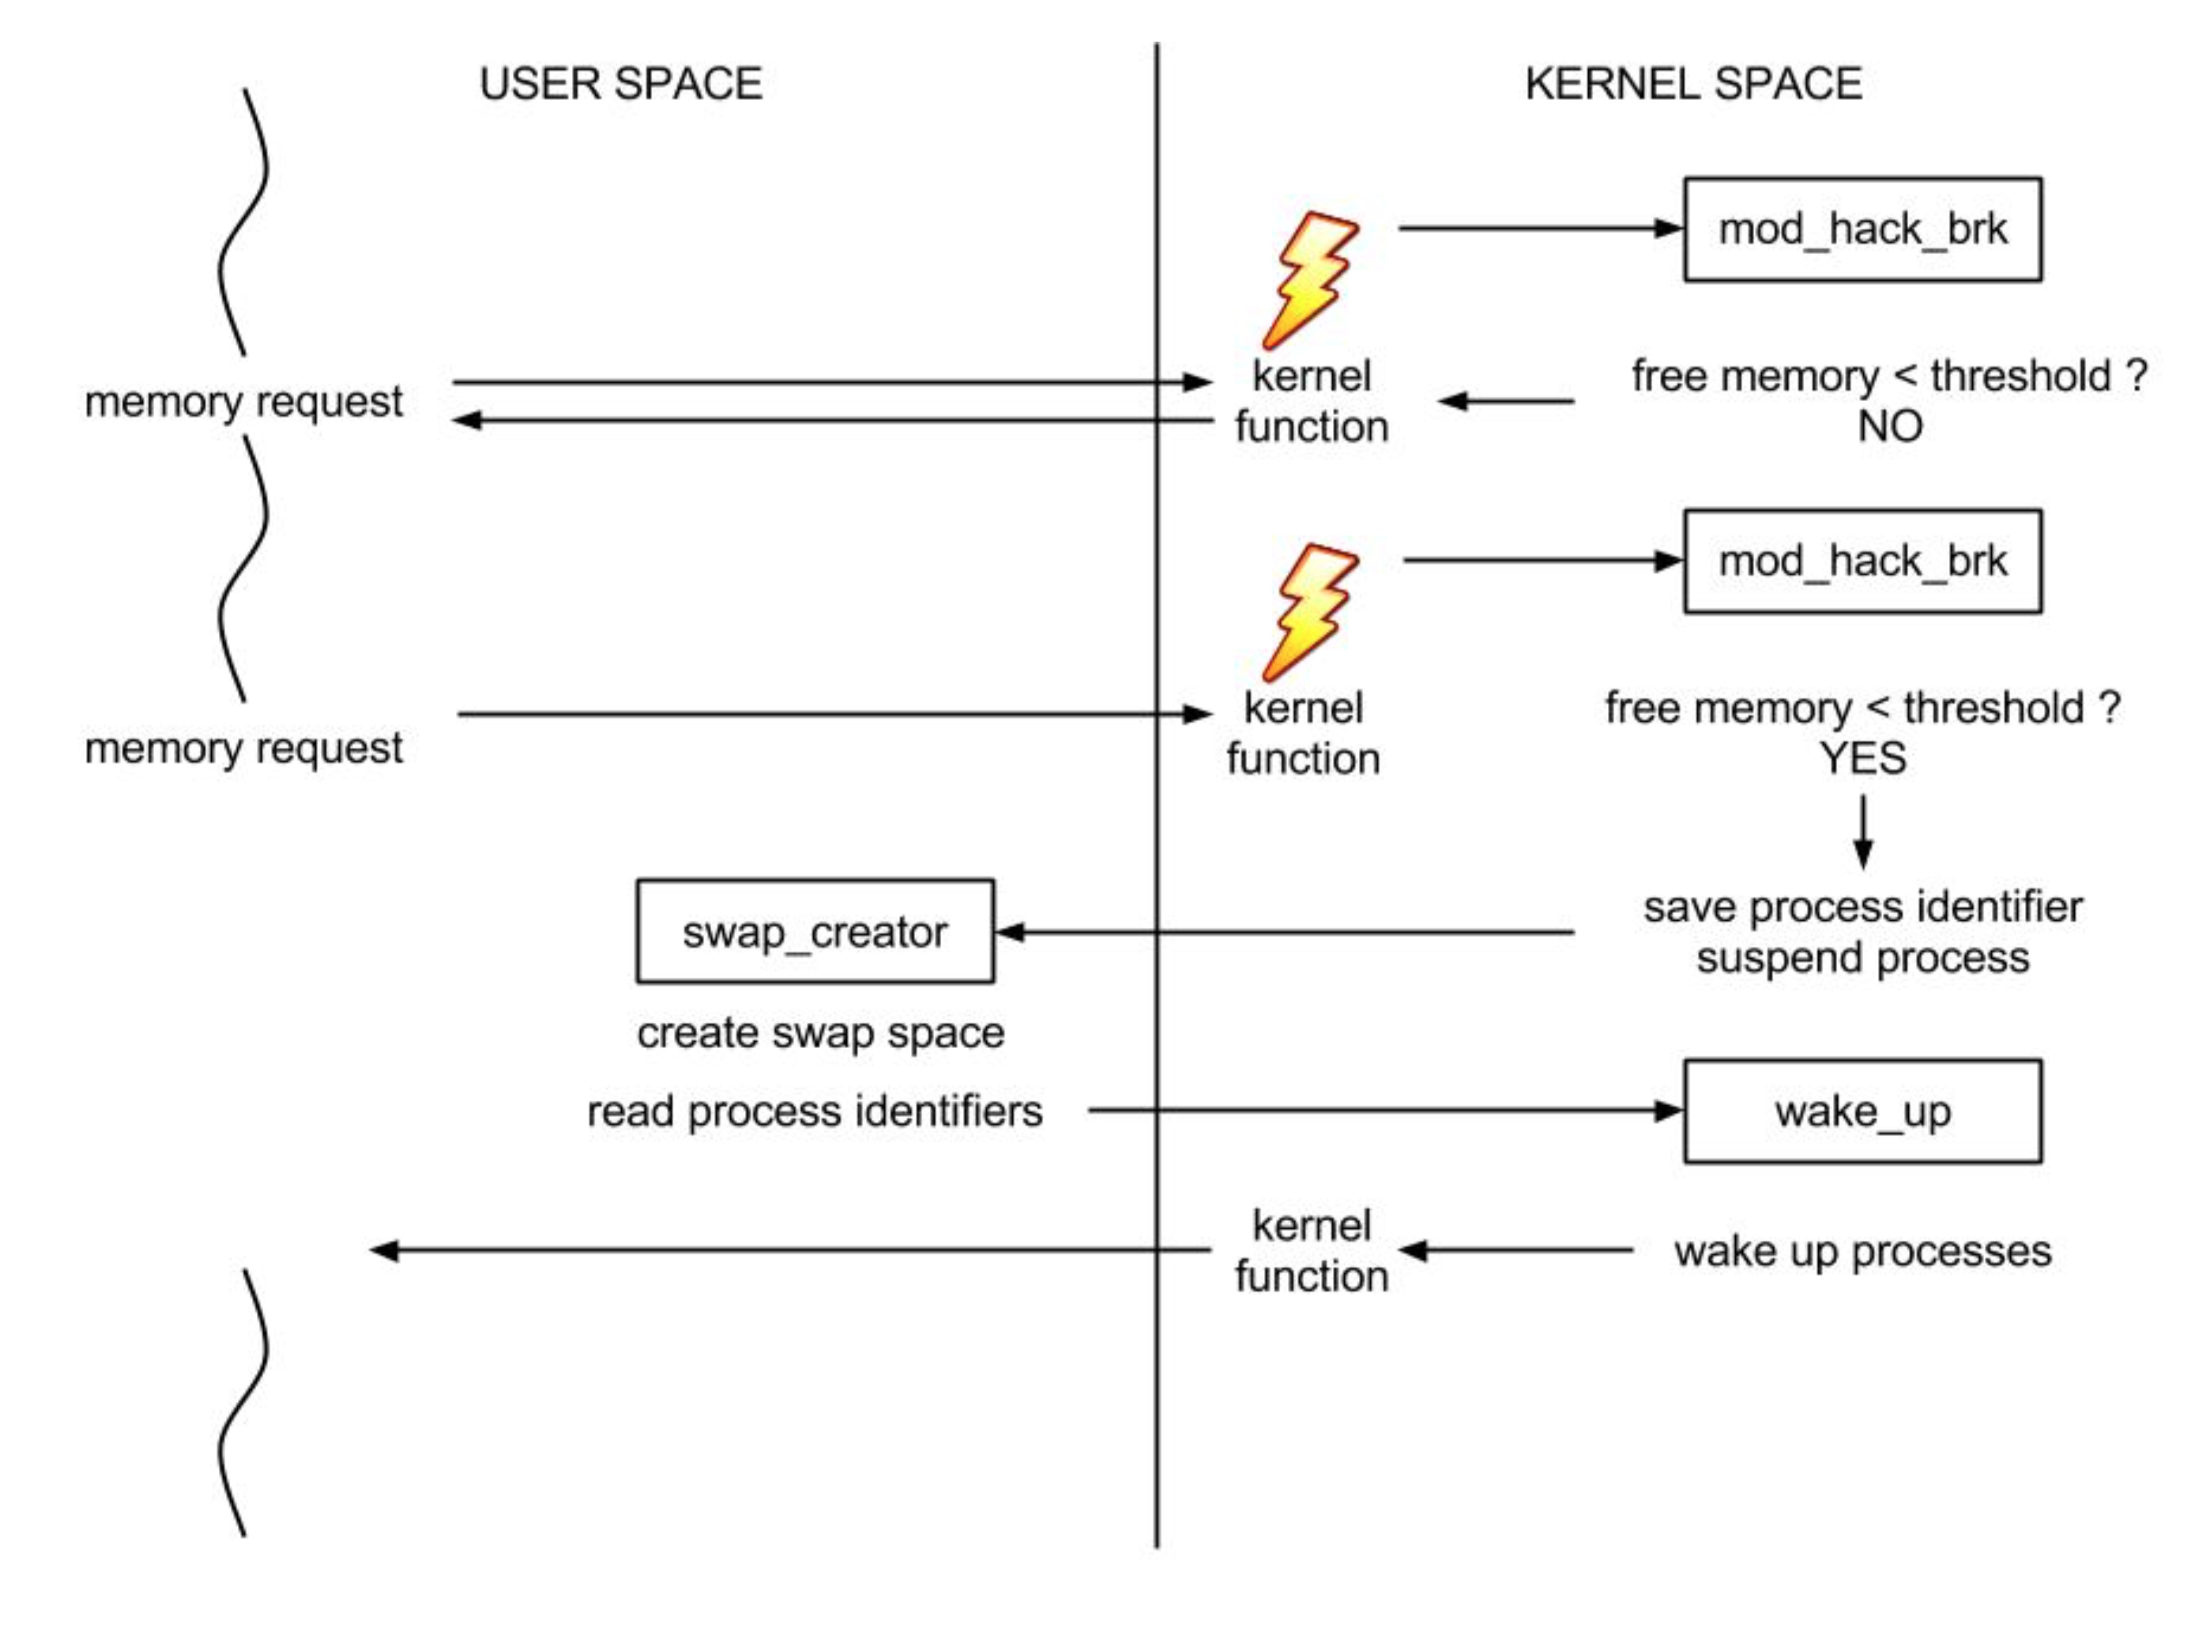
\includegraphics[width=\columnwidth]{chapter_memory_exhaustion_figures/Figure_1.png}
\caption[Design overview]{\textbf{Design overview.}}
\label{mefigure1}
\end{figure}

1) mod\_hack\_brk Module: The mod\_hack\_brk module is a kernel module that checks the
amount of free memory present in the system and checks if it is below a system-dependent
threshold. By default, the kernel sets a threshold in order to know if the machine is
in the out of memory state. This threshold is placed at 3\% of the total amount of virtual
memory present in the system. This way, the kernel has enough memory to run the \gls{oom}
Killer, if needed. The mod\_hack\_brk is more conservative and places the threshold at 7\%
of the total amount of system’s virtual memory. Hence, the swap\_creator process will have
enough memory to avoid the \gls{oom} Killer and create the swap space. In order to check the
amount of free memory we had to decide between two main directions: perform a periodic poll
or check each time a process requests more memory. The former has the main problem that it
will introduce an overhead in the system even if the system is idle. Another important drawback
of this solution is that we have to manage a trade-off between the time between polls and the
introduced overhead: if the polls are not sufficiently frequent, we may miss an out of memory
state and a user process will be killed. On the other hand, if the polls are too frequent,
the introduced overhead will be prohibitive. Thus, we decided to check the amount of free
memory each time a process requests more memory. When a process requests more memory to the kernel,
the the mod\_hack\_brk module intercepts this requests and, before any kernel function is executed,
checks the available memory in the system. This solution has the main drawback that it introduces
and overhead each time a process requests memory, but it avoids the trade-off described above regarding
the polling solution. In case the amount of free memory is below the threshold, the mod\_hack\_brk module
suspends the current process in order to prevent it from trying to allocate more memory. Then, the
module stores the process id in a configuration file and notifies to the swap\_creator process that
more swap space (i.e. virtual memory) is needed.

2) swap\_creator Process: The swap\_creator process is a process that runs with root
privileges in user space and its main function is to create a new swap space whenever
needed. During most of its lifetime, this process is sleeping and it is woken up only
when a new swap space is needed. The main reason why this is a process and this
functionality is not integrated within the mod\_hack\_brk module is that it is a bad
idea in general to open files from the kernel space. I/O operations are the source of
a large number of errors, and one of these errors in kernel space will cause the entire
system to crash. Hence, having all these operations in user space makes CUDSwap more robust.
Once this process is woken up, it performs four important steps. First, it creates a 2GB file
with no holes (i.e. it is not a sparse file and it is zeroed). Second, it creates a child
process that formats the created file as a swap space. Third, the swap creator process mounts
the created file as a swap space, increasing the amount of virtual memory. Finally, this process
reads the configuration file where the mod\_hack\_brk module had stored the sleeping process ids
and sends them to the wake\_up module.

3) wake\_up Module: The wake\_up module is a kernel module tailored to receive process
ids of sleeping processes and wake them up. The reason why this is a kernel module is
because the processes have been changed to sleeping mode in kernel space and, in order to
wake them up in a reliable manner, they should be woken up in kernel space.

\subsubsection{Implementation}\label{subme_prev_oom_i}

1) Intercepting memory requests: In the Linux kernel, there are two main system
calls that can be used by a process in order to modify its data segment: do\_mmap and
do\_brk. The most common system call used is do\_brk. In order to intercept the do\_brk calls,
we take advantage of Kprobes \cite{Krishnakumar2005}. Kprobes is a kernel debugger system that allows the
module programmer to add functions before and after a certain system call is executed.
This way, we can introduce a function before the do\_brk system call is executed and the
mod\_hack\_brk module can perform the needed checks to ensure the minimum free virtual
memory to avoid the OOM Killer calls.

2) Getting Memory Information: The easiest way to get the memory information is by
reading the \texttt{/proc/meminfo} file. Although reading a file from kernel space
is not recommended, the fact that this is a well-known file reduces the probabilities
of an I/O failure. However, there isn’t any easy way to manage files from the kernel
space because the standard libraries for manage files are not exported in kernel
space. Furthermore, in the newer kernel versions, the system calls to manage files
(\texttt{sys\_{open/read/write/close}}) are not exported. Hence, the only way to
manage file in kernel space is to go one step below and use low-level kernel functions,
using \texttt{linux/fs.h}. Since it is hard to manage files directly using this API,
we have created a simple library on top of this API that simplifies its usage and
it is as similar as possible to the standard C library API. This library is a bit
hackish because the functions defined in \texttt{linux/fs.h} expect that the buffer
address passed as parameter belongs to the user space. The addresses that we are
using are from kernel space, so these functions will fail. Our library fixes this
issue by marking our addresses as safe. This hack is done using the set\_fs function,
as shown below.

\begin{lstlisting}[language=C]
old_fs = get_fs();
set_fs(KERNEL_DS);
/* File operations */
set_fs(old_fs);
\end{lstlisting}

Once we get our library for file management, we can parse the \texttt{/proc/meminfo}
file and get all the needed information. We have created a structure, mem info
struct, which stores all the relevant memory information and facilitates the out
of memory state detection. The contents of this structure are shown below.

\begin{lstlisting}[language=C]
typedef struct{
        unsigned long ram;
        unsigned long swap;
        unsigned long ram_free;
        unsigned long swap_free;
        unsigned long cached;
        unsigned long buffers;
        unsigned long total_vm;
        unsigned long free_vm;
        unsigned long sys_threshold;
        unsigned long committed_vm;
        unsigned int oc_ratio;
} mem_info_struct;
\end{lstlisting}

3) mod\_hack\_brk - swap\_creator Communication: The mod\_hack\_brk-swap\_creator
communication is challenging because we have to perform communication from the
kernel space to the user space (on the other direction, it is straightforward: system
calls). Furthermore, the swap creator process is a root process and the active
process during the execution of mod\_hack\_brk may be a non-root process without
privileges to send a signal to a root process. However, both problems are solved
because we have access to the signal primitives. Using the signal primitives, we
can provide the entire task struct of the receiving process, and our signals do not
pass the privileges checks.

4) swap\_creator - wake\_up Communication: The swap\_creator-wake\_up communication
is easier since the sender is in user space and the receiver in kernel space. In
this case, we have decided to use the procfs API in order to send each process
id to the wake up module. The wake up module creates a new entry in the \texttt{/proc}
filesystem, and the swap creator process simply opens it and writes the process
identifier of the sleeping process.

\subsection{Performance}\label{subme_perf}

CUDSwap is a set of modules that is always running in the system, so it will be
interesting to see how it affects the overall performance of the system. Since
CUDSwap mainly affects the performance of the do\_brk call, we have coded a simple
benchmark that stresses this situation.

Our benchmark consists of a program that allocates a large amount of memory 2GB in
our tests in chunks of 1KB. It then randomizes the character present in this memory
and counts the number of characters between 0 and 9. Finally, it frees the allocated
memory. These operations are performed 20 times. This simple benchmark executes a bunch
of do\_brk, so we can notice the overhead introduced by CUDSwap. It also accesses to
all the positions in the array multiple times, so we can also notice the performance
degradation due to swapping.

We performed our evaluation in Amazon EC2 \footnote{\url{ http://www.amazon.com/ec2}}. We have selected an M1 Medium instance
with the following characteristics: 2ECU, 3.75GB memory, 410GB storage, and Linux
kernel v3.0.14. Then, we ran our test, first without CUDSwap and next with CUDSwap
running on it. The total time to run our benchmark without CUDSwap was 1183.24 seconds,
and with CUDSwap, it was 1223.27 seconds. Thus the overhead introduced by CUDSwap is quite
low, only about 1.03X slower.

The second interesting performance comparison is running our benchmark in a smaller
instance with not enough memory, creating a new swapping space and allowing it to finish.
We chose an M1 Small instance with the following characteristics: 1ECU, 1.7GB memory,
160GB storage, and Linux kernel v3.0.14. The total run time in the small instance that
included adding swap space through CUDSwap was 8845.32 seconds. If a medium instance
is chosen instead, the run time is 1223.27 seconds. Thus, the benchmark in the smaller
instance is 7.23X slower due to low performance of swapping.

Finally, we also measured the time spent to create the swap space. This time was
418.43 seconds, which is much larger than we expected. This low performance is induced
by the fact that the storage in Amazon EC2 is in EBS volumes \footnote{\url{http://www.amazon.com/ebs}}, which are attached
to an instance through the network.

\subsection{Cost Analysis}\label{subme_cost}

Since CUDSwap is tailored for the cloud environment, its evaluation has to be based
on its derived costs too. First of all, we should derive the cost per resource unit
(ECU per hour, GB of memory per hour and GB of storage per hour). In order to do that,
we will solve systems of three equations of the type:

$$
C_{cpu} ∗ P_{cpu} + C_{mem} ∗ P_{mem} + C_{disk} ∗ P_{disk} = P_{instance}
$$

Here $C_i$ and $P_i$ are the configuration and price for the resource $i$ and $P_{instance}$
is the price of the instance.

Instead of picking only three instance types and solving only one system of equations,
we pick a subset of available instances in Amazon EC2 and solve all systems of three
equations resulting from all possible permutations. Table \ref{metable1} shows the selected
configurations and their price. We used a simple Python script to generate all systems,
their solutions and average them.

\begin{table}[htbp]
\centering
\caption[Selected instance configurations]{Selected instance configurations.}\label{metable1}
\begin{tabular*}{\textwidth}{ccccc}
\toprule
Name & $C_{cpu}$ & $C_{mem}$ & $C_{disk}$ & $C_{instance}$\\
\midrule
M1 Medium & 2 & 3.75 & 410 & 0.139\\
\midrule
M1 Large & 4 & 7.5 & 850 & 0.260\\
\midrule
M1 Extra-large & 8 & 15 & 1690 & 0.520\\
\midrule
M3 Extra-large & 13 & 15 & 0 & 0.580\\
\midrule
M3 Double extra-large & 26 & 30 & 0 & 1.160\\
\bottomrule
\end{tabular*}
\end{table}

Our calculations show that the cost for each ECU per hour is \$0.012, for each
GB of memory per hour is \$0.028 and for each GB of storage per hour is \$0. We
can see that the user is charged more for memory usage than for the CPU usage.
Hence, one possible way to save user’s money is to use a smaller instance with swap
space enabled.

If we pick as an example the test run from the previous section, where the benchmark
took 8845.32 seconds (2-3 hours) in the small instance and 1223.27 seconds ($<$1 hour)
in the medium instance, we can see that the user is charged \$0.195 (3 * 0.065) in the
small instance case and \$0.130 in the medium instance. Hence, if the user knows in
advance that his memory requirements will exceed that of small instance, it is cheaper to
run the code in the medium instance than in the smaller one with swap space.

However, the common case is one where the user doesn’t know in advance the total
memory requirements. In this case, the user typically runs his code in the smaller
instance and, when it gets killed, it terminates the small instance and runs his
code in the medium instance. Using the same example as above, we note that the user
would have spent a total amount of \$0.195 (1 hour for the small instance \$0.065 and 1 hour
for the medium one \$0.130). Then, we can see that the user would have spent the
same amount of money as running the code on a small instance with swap space. In
such a case, it is better for the user to use the small instance with swap space as
that avoids the hassle of moving the application from one instance to another.
Although in this case CUDSwap don’t save user’s money, it improves the user’s
experience because she doesn’t feel that she is wasting the money on the small
instance when it gets killed.

\subsection{Conclusion}\label{subme_conclusio}

In this paper we have described CUDSwap, a set of kernel modules that prevents the memory
exhaustion failure in virtual machines in cloud computing environment. We demonstrated
that the memory oversubscription is the most expensive resource in a cloud environment
and this cost is shifted to end user. Finally, we showed how CUDSwap could improve user’s
experience in a cloud environment.

The current prototype of CUDSwap is only a preliminary prototype and has a large scope
for improvement. The first source of improvement will be to obtain the memory
information directly from the kernel routines instead of reading the \texttt{/proc/info}
file. This will improve the out of memory state detection. With the current
implementation, we may miss an out of memory state if a process tries to allocate
more than 4\% of total memory with a single call. This is because we check for
memory threshold before a memory allocation takes place, but we do not take into
account how much memory the process is going to allocate.

The second source of improvement will be the way process identifiers are shared
between the mod\_hack\_brk and the swap\_creator process. Currently, this is done
through a configuration file, but one possible approach will be using the procfs
as in the wake\_up module case. This change will completely avoid the necessity
to open files in kernel space, making CUDSwap more robust and compliant with Linux
kernel development standards.

Finally, our current performance testing of CUDSwap is quite preliminary and
limited. We need to perform an extensive evaluation of CUDSwap with a wide variety
of applications having varied memory requirements. In particular, we need to test
UDSwap with standard memory benchmarks, and perform a cost benefit analysis. This
future tests can show cases where a smaller instance with swap space is cheaper
than a bigger instance with enough memory, as well as they will allow to characterize
the situations where CUDSwap is highly useful.

% \glsresetall

\section{CUDSwap: Tolerating Memory exhaustion failures in cloud computing}\label{section_cudswap}

Cloud computing is now being used by a wide variety of users, ranging from
expert programmers and system administrators to scientists and laymen.
Cloud providers are taking full advantage of all their resources as much as
they can. Memory is the most expensive resource in terms of oversubscription
and this has resulted in high price to the end user. Furthermore, performing
swapping in \gls{vm} is expensive, so the cloud providers
usually do not offer any swapping space for their systems. As a consequence,
when a \gls{vm} runs out of memory, user processes are killed. This scenario in
cloud environment is especially critical, since the user loses all of
his/her execution time and, by extension, the money invested in this
computation. For cloud users such as life scientists with varying memory
requirements, this is a critical problem. This paper presents CUDSwap,
a kernel extension module designed to detect memory exhaustion in cloud
instances, add more swap space, and thus prevent process failures. CUDSwap
has been implemented in Linux kernel and has been evaluated over a variety
of workloads as well as real-world life science applications. The paper
describes CUDSwap design and implementation details, and reports performance
details from the evaluation.

\subsection{Introduction}\label{sub_cudswap_Introduction}

Cloud computing is being used in a wide variety of fields, including web
hosting, media content, scientific computing, and many more. This wide range
implies that the cloud users are not necessarily computing experts,
especially in the world of scientific computing that includes biologists,
physicists, chemists, etc. From our past experience working with scientists,
we have found that their experience with the cloud is often quite poor,
and sometimes they feel that they are wasting money using the cloud. Usually,
scientists do not have an a priori idea of the amount of various computing
resources they will need to complete their computing tasks. Typically,
they perform a rough estimation of the resources they will need and launch
the cloud instance that they think will be enough to run their applications.
An incorrect estimation of required resources can lead to poor performance
and even complete failure. In the case of an incorrect CPU estimation, the
application will simply take longer to finish, but the work is not lost.
In the case of incorrect storage estimation, the user can dynamically add
more storage to the instance, so that the application can continue working
without any problem.

However, the most critical resource is memory, because when it is exhausted,
the application is aborted and all the work done by the application is lost.
This is because cloud providers usually don't provide any swap space in
their instances due to high impact on the performance of
their systems. As a result, when a user's virtual machine (VM) doesn't have
enough memory to execute all the running applications, user processes are
killed in order to keep the VM alive. In Linux systems, processes are
killed using the Out Of Memory Killer (OOM Killer), a kernel module that
prevents the Out Of Memory machine state in the VM. This memory exhaustion
failure not only results in poor user experience, but also results in a large
financial loss for the user. All the work done before a process is killed is
lost and all the money invested in these processes
is wasted. Furthermore, the user has to start a new, larger VM, increasing
the total cost for the user.

In this paper, we address this memory exhaustion failure problem in VM
instances by introducing CUDSwap, an elegant kernel module that requires
minimal changes to the current Linux kernel. This module is designed to
avoid the OOM Killer calls by increasing the amount of virtual memory on
the fly. CUDSwap is a dynamic kernel module that monitors the amount of
free system memory, and adds swap space whenever needed, so that the
application process is not killed. We have implemented a prototype of
CUDSwap for Linux kernel and evaluated it extensively for a variety of
applications ranging from artificial workloads to real-world, life science
applications on Amazon EC2. This evaluation demonstrates that CUDSwap
prevents memory exhaustion failures of applications running on cloud. In
addition, CUDSwap improves user experience and even reduces the total
cost of running applications on cloud. We provide a detailed cost benefit
analysis of using CUDSwap.

By using a dynamic approach, CUDSwap uses the storage space only when it
is strictly needed. Furthermore, with increasing use of cloud in areas
beyond computer science, a large number of users do not have enough
computing background to create swap space before running their program.
CUDSwap creates swap space for them. Another advantage of CUDSwap is in
the case where a user is unable to accurately predict her program memory
requirement. In some applications, it is hard to predict the amount of
memory they will need and the user may make an incorrect approximation
that may result in provisioning insufficient memory to its processes.
CUDSwap enables such processes to complete their execution.

The remainder of this paper is organized as follows. Section \ref{sub_cudswap_Work}
provides a brief review of some important related work. Section \ref{sub_cudswap_VMs}
describes the details of how VMs manage memory exhaustion at present.
Section \ref{sub_cudswap_Design} describes the design approach of the system.
Section \ref{sub_cudswap_Implementation} describes the Linux implementation details of
CUDSwap. Section \ref{sub_cudswap_Evaluation} discusses the performance results, as well
as a cost benefit analysis. Finally, Section \ref{sub_cudswap_Conclusion} discusses
future directions and concludes the paper.

\subsection{Related Work}\label{sub_cudswap_Work}

Earlier work on memory exhaustion failures in the cloud has not been
focused on the users point of view. They are targeted to provide solutions
to the memory oversubscription problem from the provider's point of view,
i.e. the impact on the physical machine as a result of running several VMs
on it. There are mainly two approaches to this problem: VM migration and
Network Memory.

Systems that provide VM migration are Xen \cite{Barham2003},
VMWare's VMotion \cite{Nelson2005} and SnowFlock \cite{Lagar-Cavilla2009},
among others. These systems move a VM that is hosted in a machine with not
enough memory and re-deploys it in a new machine. They provide support for
reconfiguring a VM in a new physical machine with enough resources to
fulfill VM's requirements. They are tailored to support sustained periods of
memory oversubscription. The main disadvantage of this approach is the VM
downtime. In order to be able to migrate the VM from one physical machine
to another, it has to be suspended in the old machine and resumed in the
new one. Although live migration techniques allow VM migration with minimal
downtime, they still have to face the problem of network link saturation.

Systems using the Network Memory approach include Cellular Disco
\cite{Govil2000}, Cooperative Caching \cite{Dahlin1994} and Nswap
\cite{Newhall2003}, among others. These systems are designed to
support short memory overloads. They create a new level on memory hierarchy by
adding a new level of memory cache between the main memory and the disk,
located across the network. A large number of these systems use the concept
of cooperative memory, which consists of performing memory swapping across
the network. The swapped out pages are stored in remote page repositories.
Earlier research has shown that cooperative memory has better performance
that disk swap \cite{Anderson1995}. However, these systems do not support
long periods of memory oversubscription and are tailored for short bursts
of memory overloads. The performance of these
systems degrades significantly when the duration of the overload increases
due to network bottleneck.

Recently, hybrid systems have been proposed in order to take advantage of
the VM migration and Network Memory benefits. One such system is Overdriver
\cite{Williams2011}, which monitors the memory overload and creates
adaptive thresholds. Based on these thresholds, the system decides between
performing Cooperative Swap or VM migration.

However, all the above-described systems do not solve the problem of the
memory exhaustion on the client VM instance. CUDSwap differs from these
earlier approaches from the memory overload point of view. While earlier
approaches tried to overcome the challenge of memory exhaustion failure by
managing the physical memory of the host machine, we address the problem
from the guest VM's point of view. This way, we are giving the opportunity
to the end user to choose between different VM configurations knowing that
her applications will be completed and she can decide based on
performance-cost tradeoffs. In \cite{Molina2013dcdv},
we provided an analysis of this problem and proposed a preliminary
solution for it. However, that solution relies on a heuristic that can
potentially miss an Out Of Memory state, resulting in the OOM Killer being
called. The heuristic is based on the default memory threshold (3\% of the
total memory) that Linux  uses to kill a process if the system is hitting
the OOM state. Specifically, CUDSwap uses a 7\% threshold, which is checked
at the time a process requests more memory. However, it does not take into
account the amount of memory requested by the process, so if it requests
more than $7\% - 3\% = 4\%$ of the total amount of memory, CUDSwap will
miss the OOM state and the process will be killed. Here, we will describe
the improvements we have made in the design and implementation of CUDSwap
based on our experience in \cite{Molina2013dcdv}.

\subsection{Memory Exhaustion in VMs}\label{sub_cudswap_VMs}
The Out Of Memory (OOM) machine state is an undesired state where the
kernel is not able to allocate more memory because there isn't sufficient
virtual memory available, i.e. the main memory space and the swap space
(in case of its existence) are full. In this scenario, the Linux kernel
tries to free up memory using the OOM Killer \footnote{\url{http://linux-mm.org/OOM_Killer}}.
The OOM Killer is a kernel system tailored to free up memory by killing processes.

The OOM Killer is the last resource used by the kernel to free up memory,
since the kernel always tries to keep all the user processes alive.
Killing processes is a critical operation, so the OOM Killer has to decide
which process is the most appropriate to be killed. The OOM Killer is
designed in a way that it tries to free up as much memory as possible by
killing as few processes as possible (only one if it is possible), and
lose as little work done (by killed processes) as possible. In order to do
so, the OOM Killer assigns a {\it rank} for each process following a set
of rules. The rank for each process is computed in a cumulative manner.
Each process is continuously assigned points and the process that has
more points is more likely to be a candidate for termination. The process
rank is initialized with the amount of resident memory allocated by the
process. The independent allocated memory of each child process (excluding
kernel threads) is then added to the parent rank. After this, the process
rank is decreased regularly by the CPU and run times. This way, processes
running for a long time are more likely to be kept alive, fulfilling the
premise of losing the minimum amount of work done.

The rank of {\it niced}  processes is doubled because they are likely less
important. Next, processes with the {\it CAP\_SYS\_ADMIN} or
{\it CAP\_SYS\_RAWIO} capabilities have their ranks reduced, since these
processes have rights to perform system administration operations and
input/output operations, respectively. They may leave the system in an
inconsistent state if killed. Finally, the process rank is shifted by the
value in {\it /proc/$<$pid$>$/oom\_adj}, which is a user-defined value
and set to its parent value by default.

The final result of following this procedure to determine which process
to kill when needed is that the processes that are killed are less
important (niced), use lots of memory, have not so far executed for long,
and are not performing any input/output operations.

\subsubsection{OOM Checklist}

Before calling the OOM Killer, the out of memory manager should go through a checklist in order to ensure that the OOM Killer is called if and only if it is necessary. This checklist performs the following steps:

\begin{enumerate}
\item Is there enough swap space left? If yes, do not call OOM.
\item Has it been more than five seconds since last failure? If yes, do not call OOM.
\item Have we failed within the last second? If no, do not call OOM.
\item Has it been ten failures at least in the last five seconds? If no, do not call OOM.
\item Has a process been killed within the last five seconds? If yes, do not call OOM.
\end{enumerate}

This checklist ensures that the system is really out of memory and it is not, for example, waiting for I/O to complete for pages swapped to disk.

\subsection{CUDSwap Design}\label{sub_cudswap_Design}

In order to prevent calls to the OOM killer, CUDSwap needs to perform three
important functions. First, it needs to monitor the available free space
in memory. Second, it needs to suspend a process requesting new memory
whenever the available free space goes below some threshold and create
additional swap space. Finally, it needs to wake the suspended process after
additional swap space has been created. CUDSwap consists of
two main modules: {\it mod\_hack\_brk} and {\it swap\_creator} (See
Figure \ref{cudswapfigure1}).

\begin{figure}[htbp]
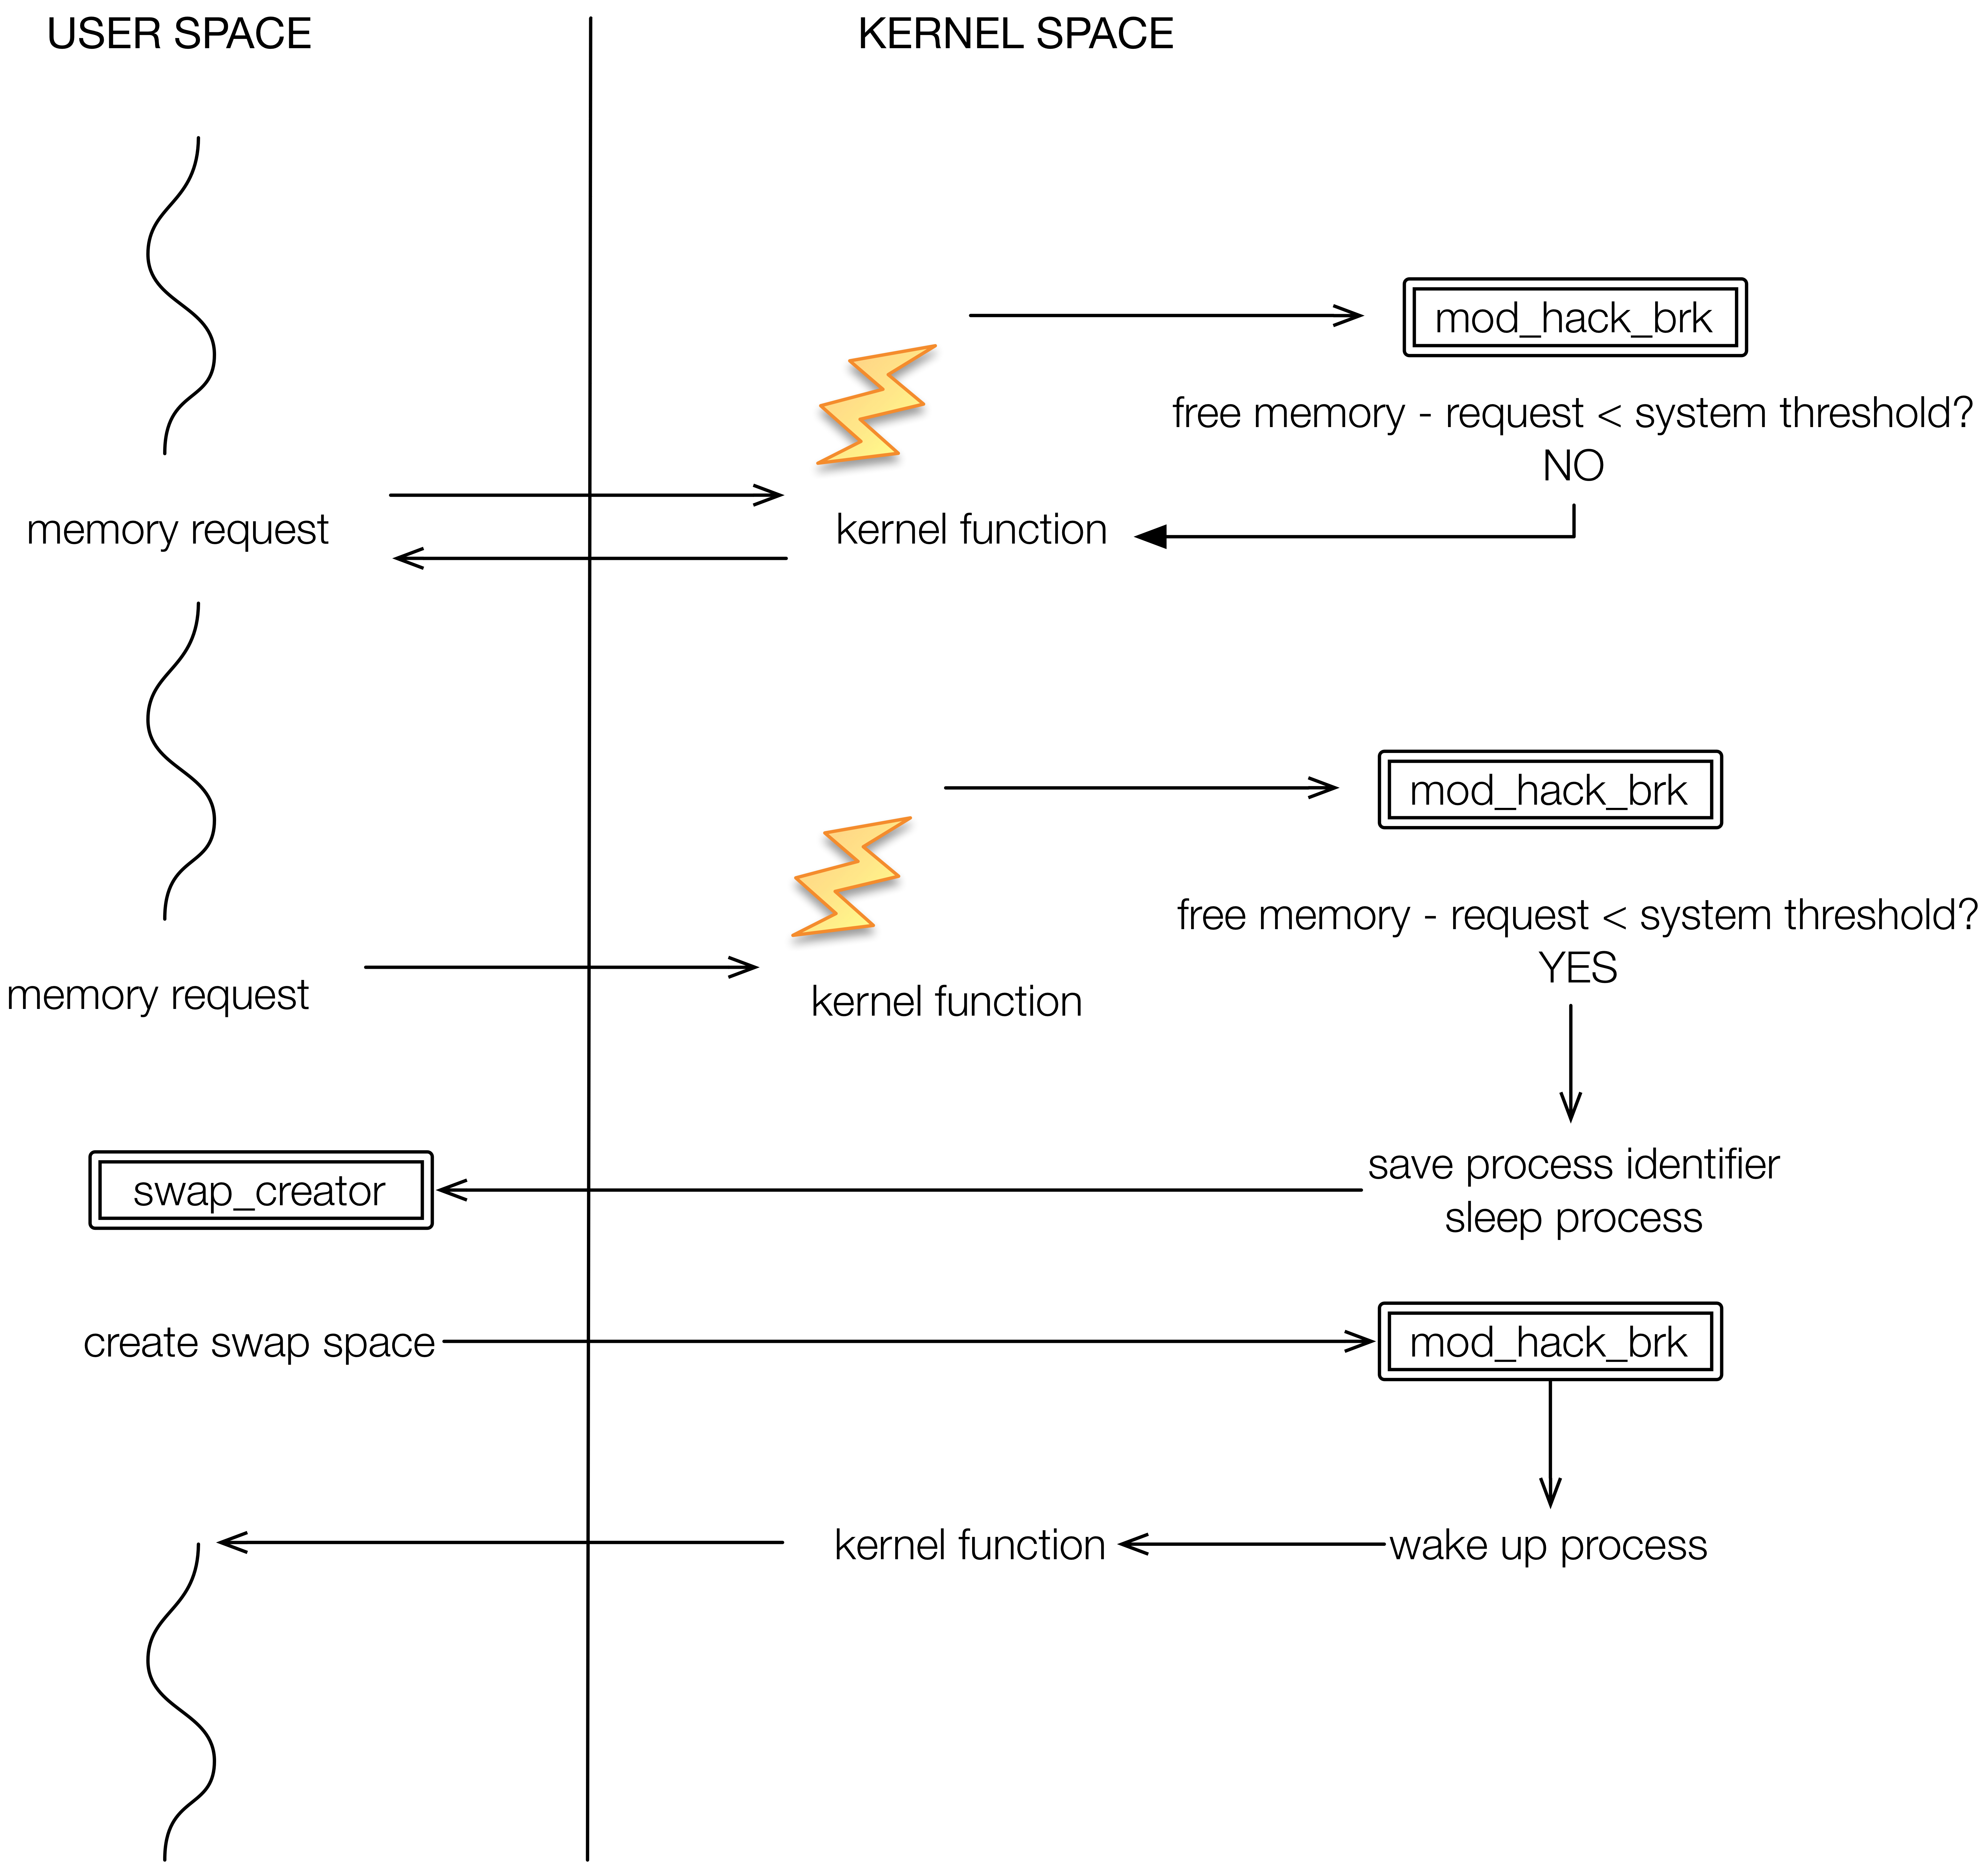
\includegraphics[width=\columnwidth]{chapter_cudswap_figures/Figure_1.jpg}
\caption[Design Overview]{\textbf{Design Overview.}}
\label{cudswapfigure1}
\end{figure}

\subsubsection{mod\_hack\_brk Module}

The {\it mod\_hack\_brk} module is tailored to monitor the free memory
of the system and suspend the current process if its current memory request
will produce a memory exhaustion failure.. By default, the Linux kernel sets a threshold in order to know if the machine is in the out of memory state. This
threshold is placed at 3\% of the total amount of virtual memory present
in the system. This way, the kernel has enough memory to run the OOM Killer,
if needed. The {\it mod\_hack\_brk} module essentially checks if the free
memory will go below this threshold if more memory is allocated to a process.

A key question is when should the {\it mod\_hack\_brk} module check whether
the amount of free memory has fallen below the threshold at 3\% of the
total amount of system's virtual memory. There are two options:
perform a periodic poll or check each time a process
requests more memory. The former has the problem that it will introduce an
overhead in the system even if the system is idle. Another important
drawback of this solution is that we have to manage a trade-off between
the polling time period and the overhead introduced due to polling: if the
polls are not sufficiently frequent, we may miss an out of memory state,
which may result in a process being killed. On the other hand, if the polls
are too frequent, the introduced polling overhead will be prohibitive.

For these reasons, we decided to check the amount of free memory each time
a process requests more memory.
Each time a process requests more memory from the kernel, the
{\it mod\_hack\_brk} module intercepts the requests and checks if the
amount of free memory in the system minus the amount of memory requested
by the process is below the system threshold. If so, it puts the requester
process to sleep, saves the process id of that process, and then
wakes up the {\it swap\_creator} module (described below) to create new
swap space. After new swap space has been created, the {\it swap\_creator}
process notifies the {\it mod\_hack\_brk} module, which wakes up all the
processes that were put to sleep. This solution ensures that only processes
that have requested more memory than available in the system are put in
sleep mode, while memory requests of processes requesting smaller amounts
of memory are satisfied.

There are two main system calls that can be used by a process to modify its
data segment: {\it do\_mmap} and {\it do\_brk}.
The {\it mod\_hack\_brk} module intercepts these system calls and, before they
are executed, checks the available memory in the system. The main drawback
of this solution is that it introduces an overhead each time the
{\it do\_brk} or {\it do\_mmap} system call is executed, but it avoids the
trade-off described above regarding the polling solution.

\subsubsection{swap\_creator Module}

The {\it swap\_creator} module is a process that runs with root privileges
in user space and its main function is to create new swap space whenever
needed. During most of its lifetime, this process is sleeping and it is
woken up by the {\it mod\_hack\_brk} module only when new swap space is
needed.

Once this process is woken up, it performs three important steps. First,
it creates a 2GB file with no holes (i.e. it is not a sparse file and it
is zeroed). Second, it creates a child process that executes the
{\it mkswap} command on the created file. Finally, the {\it swap\_creator}
process mounts the created file as a swap space, increasing the amount of
virtual memory. After this final step, this process notifies the
{\it mod\_hack\_brk} module, and goes back to sleep.

\subsubsection{Design Discussion}

The functionality of creating new swap space is implemented as a
separate module ({\it swap\_creator} module) running in the user space.
The main reason why this functionality is not integrated within the
{\it mod\_hack\_brk} module is that it is a bad idea in general to open
files from the kernel space. I/O operations are the source of a large
number of errors, and one of these errors in the kernel space will cause
the entire system to crash. Hence, having these operations in user space
makes CUDSwap more robust.

We highlight the fact that in this design, new swap space is created
strictly if it is needed, i.e. if the amount of free memory in the system
minus the amount of memory requested by the process is below the system
threshold. This is different from our earlier design \cite{Molina2013dcdv}
where new swap space was created if there was a likelihood of memory
exhaustion. After performing several experiments, we concluded that
this higher threshold is too conservative. We observed that it
resulted in wasting system resources most of the time, i.e. new swap
space was created when the available free memory would not have fallen
below 3\% and hence OOM Killer process wouldn't have been invoked.

In addition, the system design has been simplified from our earlier
design. The {\it wake\_up} module from the earlier implementation has been
removed and its functionality has been included in the {\it mod\_hack\_brk}
module. The main reason for this change was to improve security
and reliability of the system. The process identifiers are no longer
stored in a configuration file, they are stored in memory in the
{\it mod\_hack\_brk} module. This way, the process identifiers are no
longer exposed to the file system, which can be targeted by third party
applications that can modify it, adding or removing process ids, resulting
in an undesired behavior in the system. This change also simplifies the
functionality of the {\it swap\_creator} module. It no longer needs to
manage the process ids of the processes that need to be woken up.

\subsection{CUDSwap Implementation}\label{sub_cudswap_Implementation}

\subsubsection{Intercepting do\_brk and do\_mmap}

We need to not only intercept {\it do\_brk} or {\it do\_mmap} calls,
but also have access to the amount of memory that the process is requesting.
This information can be obtained using Jprobes \cite{Mavinakayahalli1006Linux}, another
flavor of Kprobes \cite{Krishnakumar2005} that gives access to the function call
parameters. Jprobes is a kernel debugger system that allows the module
programmers to add functions before and after a certain system call is
executed. This way, we can introduce a function before the {\it do\_brk}
system call is executed, and the {\it mod\_hack\_brk} module can perform
the needed checks to ensure the minimum free virtual memory to avoid
the OOM Killer calls. Using the parameters of the system call, we can
compute the amount of memory that the process is requesting, so we can
deterministically decide whether the system has enough memory to handle
the request.

\subsubsection{Getting Memory Information}

We obtain memory information directly from kernel routines. The Linux
kernel provides two different routines for getting the memory information:
{\it si\_meminfo} and {\it si\_swapinfo}. The former provides the
information of the RAM usage, while the latter provides the information of
the swap space. However, the {\it si\_swapinfo} routine is not exported to
the Loadable Kernel Module (LKM) space. We address this problem by
recognizing that the two routines have the same signature and their usage
in the LKM does not incur any security issue. Thus, we have modified the
Linux kernel source to export the {\it si\_swapinfo} routine and then use
it in our {\it mod\_hack\_brk} module. We should highlight that this is the
the only change needed in the current Linux kernel.

This process of obtaining memory information directly from the kernel
routines is a significant change from our earlier implementation that read
memory information from the {\it /proc/meminfo} file. This change completely
removes the interaction of the kernel with the file system, removing any
source of kernel failure due to this interaction.

\subsubsection{mod\_hack\_brk - swap\_creator Communication}

The {\it mod\_hack\_brk} and {\it swap\_creator} modules have to communicate
in both directions. The {\it mod\_hack\_brk} module needs to wake up
the {\it swap\_creator} module whenever new swap space is needed, and the
{\it swap\_creator} module needs to communicate with the
{\it mod\_hack\_brk} module after the new swap space has been created.
The former communication is challenging because we have to perform
communication from the kernel space to the user space. Furthermore, the
{\it swap\_creator} process is a root process and the active process during
the execution of {\it mod\_hack\_brk} may be a non-root process without
privileges to send a signal to a root process. However, both problems are
solved because we have access to the signal primitives. Using the signal
primitives, we can provide the entire {\it task\_struct} of the receiving
process, and our signals do not go through the privilege checks.

For communication from the {\it swap\_creator} process to the
{\it mod\_hack\_brk} module, the {\it mod\_hack\_brk} module creates a
new entry on the /proc virtual file system and the {\it swap\_creator} process only
writes a single value to notify that the swap space has been successfully
created. This implementation is much more secure than our earlier
implementation, since the process ids are no longer provided through the
/proc file system and the {\it mod\_hack\_brk} module can ensure that the
process ids that it has are correct and secure to use.

\subsection{CUDSwap Evaluation}\label{sub_cudswap_Evaluation}

To evaluate the performance of CUDSwap, we have used four different workloads:
\begin{enumerate}
\item Workload 1: An artificial application that executes ten times a large
chunk of memory allocation and performs a sequential write followed by a
sequential read on it.

\item Workload 2: An artificial application that allocates a large chunk of
memory and performs a random write followed by a random read on the entire
chunk of memory.

\item Workload 3: An artificial application that executes Workload 1, and
in parallel also executes a process that continuously writes a large file
to disk, in order to stress the I/O system.

\item Workload 4: A real-world, bioinformatics application. We have used
the sequence clustering step on the QIIME pipeline \cite{Caporaso2010}
using the
UCLUST algorithm \cite{Edgar2010}. This step takes a sequence file with the
input sequence and a reference file with the cluster sequence seeds. It
then parses the input file and tries to group the input sequence with
reference seeds such that they are similar above some user-defined threshold.
\end{enumerate}

In order to conduct our experiments, we have used three different instances
of Amazon EC2 \footnote{\url{http://www.amazon.com/ec2}}: Micro, Small and Medium instances. Table
\ref{cudswaptable1} shows the characteristics of these instances. We decided
to use a real cloud to conduct our experiments in order to remove the potential
infrastructure differences present in a controlled lab environment. Instead,
our controlled set of applications that exhibits different memory behaviors
(including a real-world scientific application) provides much more realistic
performance measures.

\begin{table}[htbp]
\centering
\caption[Selected instance configurations]{Selected instance configurations.}\label{cudswaptable1}
\begin{tabular*}{\textwidth}{ccccc}
\toprule
Instance & CPU & Memory & Storage & Price\\
\midrule
Micro & 1 or 2 ECU & 615 MB & EBS only & \$0.02 per hr\\
\midrule
Small & 1 ECU & 1.7 GB & 160 GB & \$0.06 per hr\\
\midrule
Medium & 2 ECU & 3.75 GB & 410 GB & \$0.12 per hr\\
\bottomrule
\end{tabular*}
\end{table}

\subsubsection{Micro vs Small Instance}
\label{micro-small}

In our first experiment, we compare the performance of running the four
workloads on Micro instance versus running them on Small
instance. For the Workloads 1, 2 and 3, we have used 1 GB of memory, which
is considerably larger than the amount of memory available on the Micro
instance. For the Workload 4, we have used a subset of 1,000,000 input
sequences from Yatsunenko human gut microbiome study \cite{Yatsunenko2012} and the
94\% representative sequence set from the GreenGenes database \cite{DeSantis2006}.
With these parameters, Workload 4 uses about 0.7 GB of memory, which is
again larger than the amount of memory available on the Micro instance.
First, we ran all four workloads on the Micro instance running standard VM
without the CUDSwap kernel extension. In all four cases, our jobs were
killed after a few minutes of execution.

\begin{figure}[htbp]
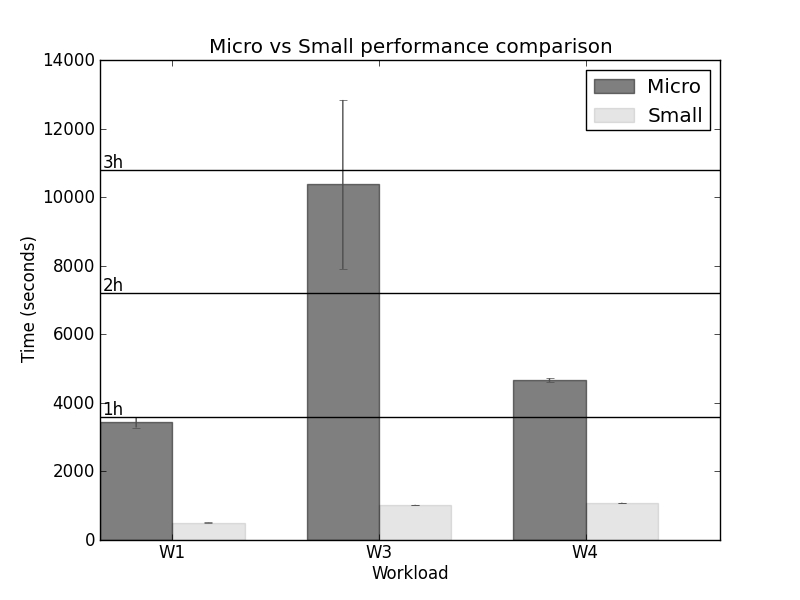
\includegraphics[width=\columnwidth]{chapter_cudswap_figures/micro_vs_small.jpg}
\caption[Comparison of the different workload performance between the Micro instance and the Small instance]{\textbf{Comparison of the different workload performance between the Micro instance and the Small instance.}}
\label{cudswapfigure2}
\end{figure}

Next, we ran the four workloads on the Micro instance and the Small instance,
in which the Micro instance VM incorporates the CUDSwap kernel extension. Figure
\ref{cudswapfigure2} shows the results obtained for different workloads.
The results of the Workload 2 are not shown in the figure for
clarity. While it took only about 8 minutes for Workload 2 to be executed
on the small
instance, it did not finish even after 20 hours in the micro instance.
This huge difference is caused by the fact that Workload 2 is designed
to remove memory locality completely. As a result,
each time the process tries to access a memory location, it is almost always
located
on the swap space, causing the system to swap pages in and out aggressively.

Our first observation is that none of our jobs on Micro instance were
killed, indicating that CUDSwap successfully created new swap space and
prevented calls to OOM killer. Of course, in each case, the execution time
on the Micro instance is considerably larger than the execution time on the
Small instance. Nevertheless, it is important to note that CUDSwap
enables completion of a job despite an incorrect estimation of memory
requirements.

Performance on the Micro instance was slower than the performance on the
Small instance by 6.73X for Workload 1, 10.14X for Workload 3, and 4.32X
for Workload 4. However, since Amazon EC2 works as a pay-as-you-go service,
we should take into account the cost of instances in our evaluation too,
in addition to the performance. From the cost information in Table
\ref{cudswaptable1}, we notice that the execution times of Workloads 1
and 4 are less than two hours, and so, using a Micro instance with CUDSwap
will be cheaper than using a Small instance (\$0.02 versus \$0.06 for
Workload 1, and \$0.04 versus \$0.06 for Workload 4).
For Workload 3, however, there is no benefit of using a Micro instance
with CUDSwap instead of using a Small instance. Most of the time they will
have the same cost (\$0.06), and sometimes the Micro instance may be more
expensive if ends up taking more than 3 hours to complete the job (\$0.08).

So, based on these workloads, we notice that CUDSwap may result in reducing
the cost to a user in some cases, but will result in higher execution times.
However, it is important to note that CUDSwap is designed for situations
where a user makes an incorrect estimation of his/her memory requirements.
In such cases, the user will start his/her job on a Micro instance, incur
the cost of Micro instance, notice that the job has been killed, and then
start the job again on a Small instance and thus incur the cost of Small
instance in addition. In this situation, the cost of running Workload 3
on Micro instance is also cheaper than the cost of running it first
on Micro instance and then later on the Small instance (\$0.06 in the first
case versus \$0.08 in the second case). Furthermore, while considering the
performance in the second case, we should also take into account the time
lost due to first running the job partially on Micro instance and then
setting up a Small instance and restarting the job. This time could be
several minutes or even more depending on when the job on the Micro instance
is killed. So, even in terms of performance, CUDSwap may result in saving
time. Finally, CUDSwap provides a better user experience. Users
(especially non-computer scientists) will typically get annoyed or
frustrated when they see their jobs being killed and losing all the
work after running for some amount time. CUDSwap avoids this situation.

\subsubsection{Small vs Medium Instance}

In order to compare the Small instance versus the Medium instance we have
changed the parameters of our workloads. In this case, for Workloads 1
and 3, we have used a chunk of memory of 2GB. Due to the results obtained
in our previous test, we have not used Workload 2 here, as it will have
very poor performance on the Small instance and we are not going to get
any benefit. For Workload 4, we have used the same subset of 1,000,000
input sequences, but we have used the 99\% representative sequence set
from the GreenGenes database. With these parameters, Workload 4 uses about
2.28 GB of memory. Again, we first ran all three workloads on the Small
instance running standard VM without the CUDSwap kernel extension. In all
three cases, our jobs were killed after a few minutes of execution.

\begin{figure}[htbp]
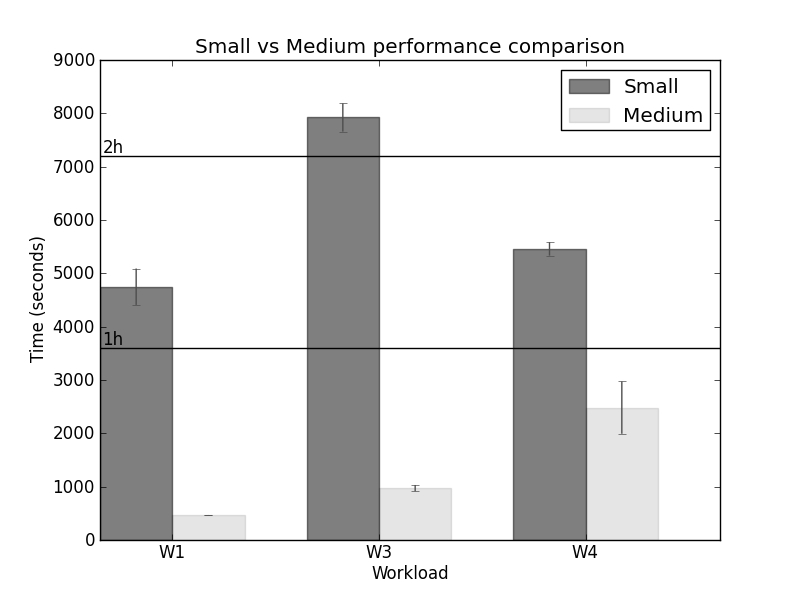
\includegraphics[width=\columnwidth]{chapter_cudswap_figures/small_vs_medium.jpg}
\caption[Comparison of the different workload performance between the Small instance and the Medium instance]{\textbf{Comparison of the different workload performance between the Small instance and the Medium instance.}}
\label{cudswapfigure3}
\end{figure}

Next, we ran the three workloads on the Small instance and the Medium instance,
in which the Small instance VM incorporates the CUDSwap kernel extension.
Figure \ref{cudswapfigure3} shows the results obtained for the
three different workloads. Again, our first observation is that none of
our jobs on Small instance were killed, indicating that CUDSwap successfully
created new swap space and prevented calls to OOM killer. Of course, in each
case, the execution time on the Small instance is considerably larger than
the execution time on the Medium instance.

Performance degradation on the Small instance in comparison to the Medium
instance is 10.01X for Workload 1, 8.14X for Workload 3 and 2.20X for
Workload 4. In terms of cost incrurred in using a Small instance with
CUDSwap versus using a Medium instance, we see that there is no advantage
of using CUDSwap. The cost is same for Workloads 1 and 4 (\$0.12) and
more expensive for workload 3 (\$0.18 for Small instance versus \$0.12 for
Medium instance). However, considering the scenario where a user first starts
his/her job on a Small instance, notices that the job is killed, and then
restarts the job on Medium instance, we see a cost advantage of using
the Small instance with CUDSwap. The cost is \$0.12 for Workloads 1
and 4 running on Small instance with CUDSwap versus \$0.18 or \$0.24 for
the Small/Medium instance scenario outlined above. Similarly, for
Workload 3, the cost is \$0.18 for Small instance and \$0.18, \$0.24 or
\$0.30 for the Small/Medium instance scenario.

In addition, the last two observations we made in Subsection \ref{micro-small}
are relevant here as well. When we take into account the time
lost due to first running the job partially on Small instance and then
setting up a Medium instance and restarting the job, CUDSwap may result in
saving time as well. Finally, CUDSwap provides a better user experience
by preventing calls to OOM killer and ensuring that the user job is
not killed even when the user incorrectly estimates his/her memory requirements.

\subsubsection{Performance Overhead of CUDSwap}

Since CUDSwap is a monitoring module that is always running on the system,
an application incurs the monitoring overhead even if it never needs
additional swap space. Thus, it is important to evaluate the performance
overhead incurred due to CUDSwap usage. Monitoring overhead of CUDSwap
comes from the inception of every {\it do\_brk} and {\it do\_mmap} calls
that the application makes. These calls are made whenever the application
requests new memory.

To estimate this overhead, we ran Workload 1 and Workload 4 on a Medium
instance under two different configurations, on a standard Linux kernel
without CUDSwap kernel extensions and on a Linux Kernel with CUDSwap kernel
extension. For Workload 1, we used 2GB of memory, and for Workload 4,
we used the same configuration as the one we used in our Small versus Medium
experiment. Workloads 2 and 3 have the same memory
allocation (memory request) patterns as Workload 1 and since CUDSwap only
interferes during the allocation process, their overhead will be same as
that in Workload 1.

Figure \ref{cudswapfigure4} shows the results of the
experiment. As we can see in the plot, performance overhead incurred
by CUDSwap is negligible (less than 1\%). This means there is no downside
to using CUDSwap continuously in the system even when the memory
requirements of the jobs have been correctly estimated by the user
and no new swap space is needed.

\begin{figure}[htbp]
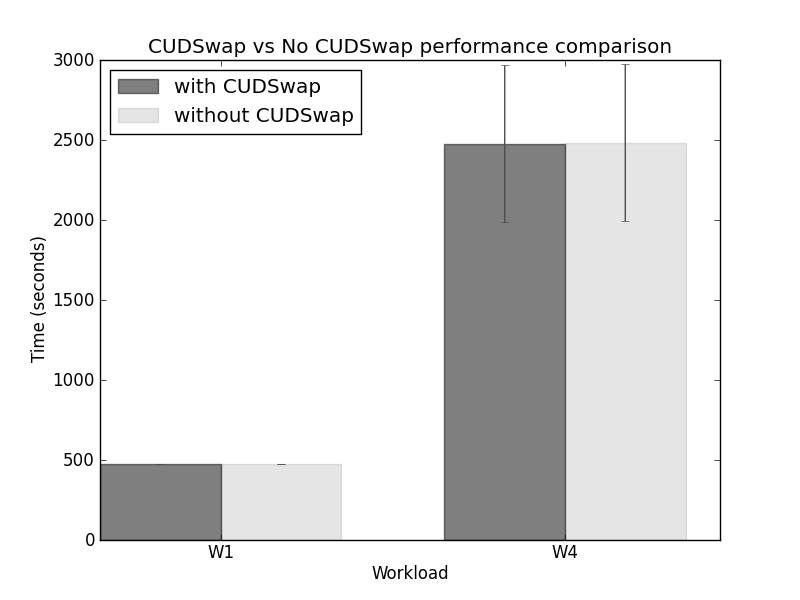
\includegraphics[width=\columnwidth]{chapter_cudswap_figures/with_vs_without.jpg}
\caption[Comparison of Workloads 1 and 4 performance on a Medium instance with and without CUDSwap]{\textbf{Comparison of Workloads 1 and 4 performance on a Medium instance with and without CUDSwap.}}
\label{cudswapfigure4}
\end{figure}

\subsection{Conclusion}\label{sub_cudswap_Conclusion}

We have presented and evaluated CUDSwap, a memory
monitor for guest operating systems that automatically adds virtual memory
to the system creating a swap space when the VM is running out of memory.
Memory is the most expensive resource in a cloud environment and
any memory oversubscription cost is shifted to the end user. Our evaluation
demonstrates that CUDSwap prevents calls to OOM killer when the VM is
short on memory by detecting this situation and adding more swap
space. Furthermore, overhead of CUDSwap is negligible under normal
circumstances when the VM has sufficient memory.

CUDSwap enables completion of a job despite an incorrect estimation of memory
requirements. This is an important functionality because it is
difficult for most cloud users to estimate accurately their application's
memory requirements. In such circumstances, users may either oversubscribe
by renting larger instances than needed, or undersubscribe by renting a
smaller instance than needed and incurring job failure. In both cases, users
end up spending more money. CUDSwap enables users to save money in
situations where users may undersubscribe. In fact, our evaluation shows
that CUDSwap also enables overall time saving for the user in case of
undersubscription, if we consider the entire duration of staring a job
on smaller instance, incurring job failure after some partial execution and
then subscribing a larger instance. So, overall CUDSwap is very useful
in terms of saving both time and money for a user who undersubscribes
due to an incorrect estimation of his/her memory requirements.

While computing with the cloud, multiple evaluation criteria should be taken
into account. Specifically, Cloud computing costs incurred by the user are
as important as the running time of the computing job.
Actual tradeoff should be left to the user. A user may choose to incur
high runtime cost on a lower budget, while another user may choose to incur
low runtime cost on a high budget.
Thus, although applications may be running up to 10X slower due to process
thrashing, the results presented on section \ref{sub_cudswap_Evaluation} show that
a user can save money. Thus, a user may choose to undersubscribe his/her
instance in favor of reducing the costs of using the cloud.

There is another subtle advantage of using CUDSwap in the form of better
user experience. In a scenario where a user encounters a failure and restarts
his/her job on a larger instance, he/she may get annoyed or frustrated
feeling that he/she has wasted time and money. CUDSwap avoids this
scenario.

In general, CUDSwap is useful only when there is difficulty in estimating the
memory requirements of a job. If a user can accurately predict his/her
memory requirements, he/she should certainly subscribe the instance
that provides sufficient memory for job completion, and not undersubscribe
and depend on CUDSwap.

CUDSwap is being used
by several graduate students in the BioFrontiers Institute at our university.
Jose Antonio Navas-Molina is a graduate student of the
BioFrontiers Institute and started working on CUDSwap after encountering
the memory undersubscription problem.
Our current implementation of CUDSwap is quite stable.
Nevertheless, there are some
additional future directions that we are addressing. At present,
CUDSwap intercepts {\it do\_brk} and {\it do\_mmap} systems calls.
Another way of consuming memory in the system is by a forking new
process, which creates a new process and a new chunk of memory needs to
be allocated for the new process. This situation can also be detected using
the Jprobes system and we plan to incorporate it in CUDSwap in the future.

Another area that we plan to investigate is the utility of CUDSwap
for applications that have widely varying memory requirements with
very short periods of peak requirements. In the absence of CUDSwap, a user
will have to subscribe a larger instance to satisfy these peak requirements.
With CUDSwap, it may be more optimal to subscribe a smaller instance, since
the time in actual swapping will be short.

\subsection{Acknowledgments}

Jose Antonio Navas-Molina is supported by the Balsells fellowship.

\section{Addressing memory exhaustion failures in Virtual Machines in a cloud environment}\label{section_memory_exhaustion}
Add paper: ``Addressing memory exhaustion failures in Virtual Machines in a cloud environment''. J. A. Navas-Molina, S. Mishra. \emph{43rd Annual IEEE/IFIP International Conference on Dependable Systems and Networks}, 2013, DOI: 10.1109/DSN.2013.6575330.
\section{CUDSwap: Tolerating Memory exhaustion failures in cloud computing}\label{section_cudswap}
Add paper: ``CUDSwap: Tolerating Memory exhaustion failures in cloud computing''. J. A. Navas-Molina, S. Mishra. \emph{International Conference on Cloud and Autonomic Computing}, 2014, DOI: 10.1109/ICCAC.2014.12.

\chapter{Meta-analyses: importance, challenges and solutions}\label{chapter_qiita}
\glsresetall
A unifying theme in the work presented in section~\ref{section_contributions}
is that it takes advantage of previously published datasets to increase the power
of the findings. The Komodo Dragon paper \cite{Hyde2016} compared new findings
on captive Komodo dragons with wild amphibians \cite{Kueneman2014} and humans and
pets living in homes \cite{Lax2014} to hypothesize that the lack of interactions
with an open environment can negatively affect human and animal health. The \gls{emp}
\cite{Gilbert2010, Gilbert2014, Thompson2017} combined samples from 97 independent
studies to answer spatial, temporal and evolutionary microbial community questions at a global scale.
The \gls{agp} used previous studies to show that the findings resulted from citizen-science
microbiome research can replicate previous results and, move research forward
by creating a massive dataset of human samples that can be used to
generate new hypotheses. Finally, the manuscript about correcting microbial blooms
\cite{Amir2017Bloom} used previously published datasets to describe a new technique
used to reduce technical differences caused by sample shipping at room temperature.

This technique of using multiple datasets (published or not)
to improve the findings of a study is known as a meta-analyses. As shown
by the previous examples, meta-analyses is a powerful tool that is becoming increasingly
common on microbiome research \cite{Lozupone2007, Ley2008, Sinha2017}. However,
this extra power comes with its own set of challenges that can delay the publication
of the results from months (as in the Komodo Draogn manuscript) to years (as in
the \gls{emp} manuscript). Namely, this challenges can be grouped in three topics:
(1) technical differences, (2) data availability, and (3) data standardization.

Technical differences are a result of differences on handling the samples, and
they can originate in any step of the proces: from decisions about sample collection and
preservation \cite{Song2016}, the \gls{PCR} primers or sequencing platform of choice
\cite{Kuczynski2011, Tremblay2015}, or even the laboratory in which the samples
are processed \cite{Sinha2017}. These technical differences can overpower
the underlying biological differences, making meta-analyses almost impossible. Thus,
it is critical that this information is captured and made available at publication
time, so other researchers can reproduce the results and/or decide if they can use
the published data in a meta-analyses with their own samples.

The second challenge presented to a researcher wanting to perform a meta-analysis
is collecting the data of the previously published results. Although current publishers
usually require the data to be deposited in a long-term repository such as
the \gls{ebiena}, there are no mechanisms that ensure that the data deposited is valid
or complete. Besides the DNA sequence data, the researcher must also track down
the metadata describing the samples. Even when the metadata publicly available,
it may be incomplete and/or the specific encoding may not
be clear for other users, requiring communication with the original authors to
decode the information.

Finally, the researcher wanting to perform meta-analyses needs to combine and normalize
his/her data with the previously published data to perform such meta-analyses.
Although standards exist to represent sample metadata, such as the \gls{mimarks} standard
\cite{Yilmaz2011}, they are not enforced by the long-term repositories or even required.
This process of normalizing metadata is tedious and hard to automate, increasing
the risk of introducing errors in the metadata which can alter the results
of the meta-analyses. Apart from the metadata, the DNA sequence data itself may
not be normalized. Sequence data available in the long-term repositories is not ensured
to be the raw data. Preprocessing performed on those
sequences, such as quality control, can introduce technical differences that affect
the results of the meta-analyses and reduce ability to find biological differences.

Section~\ref{section_qiita} presents Qiita, a web-based service designed to
alleviate the meta-analyses challenges by enforcing standards, requiring sample
handling information, normalizing raw data representation and processing and hosting
over 150,000 samples publicly available from around the world. The material in section~\ref{section_qiita}
is submitted for publication in \textsl{Nature Methods}. As a first
co-author of this publication, I have been involved in the design and implementation of
the database, graphical user interface and plugin system of Qiita and wrote the text.

\section{Qiita accelerates microbiome meta-analyses from months to minutes}\label{section_qiita}
Add paper: Qiita paper (in prep).

\chapter{Making meta-analysis accessible to the clinician}\label{chapter_rapid_response}
\glsresetall
\section{From sample to multi-omics conclusions in under 48 hours}\label{section_48hours}
\section{PlateMapper}\label{section_platemapper}

\chapter{Conclusions}\label{chapter_conclusions}
\glsresetall
% \chapter{Conclusions}\label{chapter_conclusions}
\glsresetall

As I described in Chapter~\ref{chapter_overview}, improvements in current technology
are pushing microbiome science to become a ''Big Data`` field. Big Data is being
generated in multiple ways. First, advances in sequencing technologies can
generate four orders of magnitude more data than 10 years ago. Second, the need
for different 'omics technologies to study different aspects of the system requires
aggregation of even more data per sample than ever before. Finally, the complex
interactions of the microbes with their niche require an accurate description of
their niche, represented in the form of sample metadata. This rapid increase of
data volume and heterogeneity presents a wide range of challenges to investigators, many of whom, due to
the various conditions and system for which the microbiome is important, are not
microbiologists by training or do not have extensive background in microbial
ecology, or in the tools that can be used to analyze the data. Some of these tools
can prove intimidating to those with no background in computer science. This
thesis provides solutions to some of these challenges, specifically by improving
usability of analysis tools and access to resources required to run those tools,
and by providing solutions to standardize data handling, storage, and analysis.

\section{Improving usability of analysis tools}

Of the tools available to perform microbiome analyses, \gls{qiime} is a choice
popular in the community. \gls{qiime} is a collection of command line scripts that
can be challenging to use for investigators who are not familiar with the \gls{cli}.
Section~\ref{section_book} described the first gold standard approach for microbiome data
analysis, starting from sample preparation and going through to publication-quality
figures. This section is a step-by-step guide, so even researchers who lack \gls{cli}
familiarity can successfully perform their analyses.

A \gls{cli} is prone to user error. A simple typographical error can make the script fail or
generate undesired results. To assess this issue (among many others), Qiita
(Section~\ref{section_qiita}) was presented as a web-based solution that allows
command execution with a \gls{gui}, minimizing the amount of input provided by
the user and removing typographical errors.

Tool developers typically focus on solving a complex problem and making their
tool available to the community as soon as possible. Developing a \gls{gui} doubles
the development time \cite{Myers1992}, a cost that developers do not want to incur
in a fast changing field like microbiome research. Qiita builds a bridge between
the developers and biologists, freeing up the developers from building a \gls{gui},
but still providing an intuitive \gls{gui} for non command line-savvy researchers.
Tool developers just provide information about the inputs and outputs of their
commands and Qiita automatically generates a web-based \gls{gui}.

This ability to make new command line tools rapidly available to non command line
savvy researchers will push microbiome research forward faster than ever before.
The usual steep learning curve for a new tool gets completely removed, because all
tools in Qiita are based on the same \gls{gui}, and the researcher can focus on
the science of their results rather than on the specifics of a new \gls{cli}.
This will enable researchers to perform all their multi-omics analyses in a
single platform, with a common user interface, facilitating advances in
multi-omics analyses likely to be critical for making the microbiome an integral
part of precision medicine. For example, mass spectrometry analyses have
historically been able to be done only by those with specific training.
Leveraging the Qiita plugin system will bring this type of specialized data analysis
to the researcher, who can then combine mass spectrometry data with other data types,
such as microbiome sequence data (both marker gene and whole genome shotgun), host
genome sequence data, and proteomics data, among others. The potential for
providing a more complete picture than ever before possible places Qiita at the
forefront of techniques that facilitate the future of microbiome multi-omics research.

\section{Improving resource utilization of analysis tools}
Section~\ref{section_bottlenecks} identified one of the common bottlenecks when
analyzing target gene sequencing data: sequence clustering. The microbiome field
has been gaining interest from computational biologists, constantly presenting in
the literatur new tools that increase the quality of the results and reduce the
time to solution. Section~\ref{subsection_openref} presented a benchmark of
available sequence clustering tools, and provided a comparative framework
that can be used to compare new tools as they become available. This framework can
objectively assess the quality and speed of new tools, enabling users to
critically assess the best tool they want to use. This empowers users with the
ability to choose a tool not based on the promises made in a specific publication,
but rather on the actual results in well-described datasets with a different range of
characteristics.

As the microbiome field keeps generating more and more data, analyzing the data
using modern laptops or personal computers is becoming an impossible task. However,
microbiologists do not necessarily have access to supercomputers, and they often
rely on cloud services such as Amazon \gls{ec2} to perform their analysis. Being an \gls{iaas}
cloud solution, microbiologists are presented with the challenge of choosing adequate
resources to run their analysis tools. In Chapter~\ref{chapter_cudswap}, I showed
that memory is the most critical cloud resource because it is the most expensive
cloud resource, and a shortage of memory translates into termination of the user's
analysis and a loss of all work performed until that point. In Section~\ref{section_memory_exhaustion},
I describe a potential solution to this problem: CUDSwap, a \gls{lkm} that monitors
the system memory and dynamically adds swap space if the system memory falls below
a given threshold. Section~\ref{section_cudswap} presented an implementation of
the previous design, removing the necessity to use an arbitrary user-defined threshold, and
evaluated the performance of CUDSwap using a memory bounded step of the
microbial analysis pipeline: sequence clustering. The sequence clustering step
follows a semi-sequential memory access pattern that makes it suitable to use
swap space under memory oversubscription situations, allowing the process to
finish at the expense of a small increase of running time. CUDSwap is a system
that improves user experience and increases the value of the resources by providing
useful results from all computations. However, CUDSwap should not be used all the time,
but rather as a safeguard when a mis-prediction occurs.

Historically, many tools for analyzing microbiome data have been developed by biologists
who acquired programming knowledge later in their careers. As the field moves towards big data,
more and more computer scientists have been involved in the development of these
tools, applying techniques and optimizations that allow tools to operate on modern
data scales. However, few developers acknowledge the big data nature of the field, and
as a result, many tools are limited to small
datasets, and do not scale well to large scale initiatives like the \gls{emp}
(Section~\ref{subsection_emp}) or the \gls{agp} (Section~\ref{subsection_ag}). To
achieve the levels of scalability needed by these initiatives, applying just pure
computer science optimization techniques or just domain specific optimizations is
not enough. A multidisciplinary team of developers is needed, in which computer
scientists can contribute algorithmic, user interface, and software engineering optimizations and domain experts can provide
a better understanding of the nature of the data to find new ways of approaching
the computational problems. This approach, as shown in sections~\ref{subsection_openref}
and~\ref{subsection_deblur}, can generate analysis tools that scale to dataset
sizes never before thought possible, enabling researches to push microbiome
research forward to a whole new level.

\section{Standardization of metadata and analysis}

Accurately describing the environment that a sample comes from is key to characterize
the microbiome of the sample and its interactions with its environment. Using a
standard to represent this information, such as the \gls{mimarks} standard \cite{Yilmaz2011},
allows researches to perform comparative analyses across multiple datasets,
improving their ability to find new relationships between the microbiome and its
niche. In Chapter~\ref{chapter_qiita}, I described how meta-analyses move microbiome
research forward by increasing the power of the findings. However, a researcher
performing a meta-analysis should ensure that the samples have been handled,
processed and analyzed in the same way, to reduce the impact of technical
differences. In Section~\ref{section_qiita}, I presented Qiita, a system
designed to facilitate meta-analyses by normalizing sample metadata and minimizing
processing differences. Qiita simplifies the complex process of creating a
meta-analysis to a few mouse clicks, cutting down the time and effort spent by
researchers from months to few minutes. This ability to easily contextualize samples
with massive initiatives like the \gls{hmp}, \gls{emp} and \gls{agp} opens the door
to a whole new world of possibilities, empowering researchers with new ways of
looking at their data and finding new links between the microbiome and their niche.
For example, researchers can find new links between the microbiome and diseases,
develop new microbiome-based treatments, or engineer new biofuels. With the microbiome
being important in so many fields, the possibilities are endless.

In current microbiome studies, researchers still spend a fair amount of time generating
metadata. In several aspects, the information should be encoded using a specific
vocabulary or ontology, and the usage of those standardized vocabularies is not
necessarily intuitive, and requires a fair amount of previous knowledge of the
specific ontology to complete the sample metadata efficiently. In Section~\ref{section_platemapper},
I presented LabMan, a system built on top of Qiita that facilitates the
process of recording the sample preparation information. This system normalizes
the representation of the sample preparation information as the wet lab technician
is performing the sample preparation. This system reduces the effort that researchers
have to spend normalizing the data, and it minimizes the human error introduced when
translating the wet lab preparation notes to the actual preparation information
file. Being able to rely on a standardized set of information enables researchers
to automate parts of the analyses. For example, as shown in Section~\ref{section_platemapper},
an initial analysis of the data can be performed automatically, providing
researchers with an initial overview of the data that can be used to guide further
downstream analyses, or to detect problems with sample processing, reducing down
detection time and, hence, the reprocessing of the samples.

LabMan helps researchers to store sample preparation information. However,
work still needs to be done to help researchers to provide their sample metadata.
A new system that guides the researchers through the \gls{mimarks} standard and
allows them to efficiently use the existing ontologies to encode their
information would greatly increase the efficiency of microbiome research.
This way, the tedious problem of formatting the sample metadata can be reduced
from weeks of effort to hours, and ideally would be performed at the same time
that the samples are collected. With such a system working jointly with Qiita and
LabMan, researchers could focus on the science and biological questions,
rather than spending months of their time on basic data formatting.

\section{Bringing microbiome research to the clinic}

The standardization of sample handling, processing, analysis, and metadata curation,
as well as improvements in the efficiency of data processing not only provide a
common platform for microbiome research, but also increases efficiency and allows
researchers to generate results at speeds never achieved before. In Section~\ref{section_48hours},
I show how combining the improvements in the tools with a group of experts can
generate multi-omics results in as little as 48 hours. These speeds provide the
opportunity for microbiome analysis to be used in areas in which time is critical.
One such area is human health, in which a multi-omics, microbiome-based analysis
can provide new relevant information to the clinicians, enabling them to diagnose
difficult cases. For example, sequencing can be used to understand \emph{Mycobacterium tuberculosis}
outbreaks \cite{Guthrie2017}, enabling researchers to identify specific mutations
and even the origin of the outbreak. Current diagnostic techniques to find the
best treatment are culture-based and can take up to 8 weeks to provide a definitive
answer. Empowering clinicians with sequencing information that generates results in
less than 8 weeks while identifying possible drug resistance genes present in the
\emph{Mycobacterium tuberculosis} strain infecting the patient will be an invaluable
resource that can save lives. This is just one example, but with the microbiome
being linked to other conditions like diabetes, Parkinson's, Autism, depression,
and many others, the potential of improving the current health care would reach a completely
new level. Furthermore, with antibiotic resistance becoming an increasing problem,
being able to treat patients with targeted antibiotics rather than broad-spectrum antibiotics
will combat this pressing problem.

This thesis provides an efficient and extensible framework for multi-omics analyses.
As new microbiome studies are being designed targeting specific links between the
microbiome and disease, this framework becomes an invaluable resource for human
health. With an increasing pool of samples available in Qiita, techniques such as
neural networks or other machine learning approaches could be applied to find new
biomarkers that facilitate patient diagnosis. New, non-invasive approaches could
be used to diagnose diseases. The microbiome is becoming a key component of precision
medicine, and providing a framework that enables faster advances in microbiome
research will help to accelerate the use of the microbiome in the clinic.


\appendix
\include{appendix}

%% END MATTER
\printindex %% Uncomment to display the index
% \nocite{}  %% Put any references that you want to include in the bib
%               but haven't cited in the braces.
% \bibliographystyle{alpha}  %% This is just my personal favorite style.
%                              There are many others.
\bibliography{references}
\bibliographystyle{plain}

\end{document}
